\documentclass[10pt,twocolumn,superscriptaddress,aps,amsmath,amssymb,citeautoscript,floatfix,prx]{revtex4-2}
\pdfoutput=1
\usepackage[english]{babel}
 
\usepackage{letltxmacro}
\usepackage{latexsym}
\usepackage{booktabs}
\usepackage{siunitx}
\usepackage{multirow}
\usepackage{algpseudocode}
\usepackage{array}
\usepackage{tabularx}

\sisetup{
  separate-uncertainty = true,
  table-number-alignment = center
}
\LetLtxMacro{\ORIGselectlanguage}{\selectlanguage}
\makeatletter
\DeclareRobustCommand{\selectlanguage}[1]{%
  \@ifundefined{alias@\string#1}
    {\ORIGselectlanguage{#1}}
    {\begingroup\edef\x{\endgroup
       \noexpand\ORIGselectlanguage{\@nameuse{alias@#1}}}\x}%
}
\newcommand{\definelanguagealias}[2]{%
  \@namedef{alias@#1}{#2}%
}
\makeatother
 
\makeatletter
\def\maketitle{
\@author@finish
\title@column\titleblock@produce
\suppressfloats[t]}
\makeatother
 
\definelanguagealias{en}{english}
\definelanguagealias{English}{english}
\usepackage{graphicx}
\usepackage{amsmath}
\usepackage{amsfonts}
\usepackage{amssymb}
\usepackage{amsthm}
\usepackage{cancel}
\usepackage{mathtools}
\usepackage{bm}

\usepackage[percent]{overpic}
\usepackage[dvipsnames]{xcolor}
\usepackage{soul}
\usepackage{wasysym}
\usepackage{dsfont}
\usepackage{physics}
\AtBeginDocument{\RenewCommandCopy\qty\SI} 
\usepackage{hyperref}
\hypersetup{colorlinks,allcolors=black}
\usepackage{comment}
\usepackage{enumitem}
\usepackage{textgreek}
\usepackage{paper-ai}
\usepackage{tcolorbox}
\usepackage{xcite}
 
\newcounter{alg}
 
\hypersetup{
  colorlinks   = true,
  urlcolor     = blue,
  linkcolor    = blue,
  citecolor    = red
}
\usepackage[mathscr]{euscript}
 
\usepackage{varwidth}
\usepackage[lined,boxed,ruled,norelsize,linesnumbered]{algorithm2e}
\usepackage{verbatim}
\usepackage[normalem]{ulem}
\usepackage{cleveref}
 
\renewcommand{\algorithmicrequire}{\textbf{Input:}}
\renewcommand{\algorithmicensure}{\textbf{Output:}}
 
% ============================================================
%  Theorem-like environments
% ============================================================
\newtheorem{theorem}{Theorem}
\newtheorem{result}{Result}
\newtheorem{lemma}{Lemma}
\newtheorem{problem}{Problem}
\newtheorem{proposition}{Proposition}
\newtheorem{remark}{Remark}
\newtheorem{assumption}{Assumption}
\newtheorem{definition}{Definition}
\newtheorem{fact}{Fact}
\newtheorem*{lemma*}{Lemma}
\newtheorem{corollary}{Corollary}
\newtheorem*{theorem*}{Theorem}
\newtheorem{thm}{\protect\theoremname}
\theoremstyle{plain}
\newtheorem{lem}{\protect\lemmaname}
\theoremstyle{plain}
\newtheorem{rem}[thm]{\protect\remarkname}
\theoremstyle{plain}
\newtheorem*{lem*}{\protect\lemmaname}
\theoremstyle{plain}
\newtheorem*{thm*}{\protect\theoremname}
\theoremstyle{plain}
\newtheorem{prop}[thm]{\protect\propositionname}
\theoremstyle{plain}
\newtheorem{cor}[thm]{\protect\corollaryname}
\newtheorem{defn}{Definition}
\newtheorem{prob}[thm]{Problem}
\newtheorem{notation}[thm]{Notation}
 
\newtheorem{manualtheoreminner}{Theorem}
\newenvironment{manualtheorem}[1]{%
  \renewcommand\themanualtheoreminner{#1}%
  \manualtheoreminner
}{\endmanualtheoreminner}
 
\renewcommand{\thealg}{\arabic{alg}}
\newtcolorbox[use counter=alg,
              crefname={algorithm}{algorithms},
              Crefname={Algorithm}{Algorithms}]
{alg}[2][]{%
  floatplacement=#1,
  float,
  colback=cyan!5!white,
  colframe=cyan!50!black,
  colbacktitle=cyan!85!black,
  fonttitle=\bfseries,
  title=Algorithm~\thealg: #2
}
 
\renewcommand{\topfraction}{0.95}
\renewcommand{\bottomfraction}{0.95}
\renewcommand{\textfraction}{0.05}
\renewcommand{\floatpagefraction}{0.9}
\setcounter{topnumber}{10}
\setcounter{bottomnumber}{10}
\setcounter{totalnumber}{20}
 

\NewDocumentCommand{\hyh}{m}{\textcolor{purple}{[HYH: #1]}}
\definecolor{mycrimson}{HTML}{A60808}
\NewDocumentCommand{\elo}{m}{\textcolor{mycrimson}{[ELO: #1]}}
\NewDocumentCommand{\sfy}{m}{\textcolor{teal}{[SFY: #1]}}
\newcommand{\EPR}{\mathrm{EPR}}
\newcommand{\eq}[1]{\begin{equation}#1\end{equation}}
\newcommand{\eqs}[1]{\begin{equation}\begin{split}#1\end{split}\end{equation}}
\newcommand{\eqnref}[1]{Eq.\,\eqref{#1}}
\newcommand{\figref}[1]{Fig.\,\ref{#1}}
\newcommand{\tabref}[1]{Tab.\,\ref{#1}}
\newcommand{\secref}[1]{Sec.\,\ref{#1}}
\newcommand{\appref}[1]{Appendix\,\ref{#1}}
\newcommand{\refcite}[1]{Ref.\,\cite{#1}}
\newcommand{\ii}{\mathrm{i}}
\newcommand{\ee}{\mathrm{e}}
\newcommand{\cd}[1]{c^{\dagger}_{#1}}
\newcommand{\cc}[1]{c_{#1}}
\newcommand{\moy}[1]{\langle #1 \rangle}
\newcommand{\sandwich}[3]{\mbox{$ \langle #1 | #2 | #3 \rangle $}}
\newcommand{\red}[1]{{\color{red} #1}}
\DeclareMathOperator*{\bigrarrow}{\rightarrow}
\DeclareMathOperator*{\biglongrarrow}{\longrightarrow}
 
\setlength{\belowcaptionskip}{-10pt}
\setlength{\skip\footins}{24pt}
\raggedbottom
 
\usepackage{bbm}
\usepackage{tikz-cd}

\newcommand{\C}{\mathbb{C}}
\newcommand{\R}{\mathbb{R}}
\newcommand{\N}{\mathbb{N}}
\newcommand{\Z}{\mathbb{Z}}
\newcommand{\End}{\mathrm{End}}
\newcommand{\Hom}{\mathrm{Hom}}
\newcommand{\Lie}{\mathrm{Lie}}
\newcommand{\ad}{\mathrm{ad}}
\newcommand{\id}{\mathrm{id}}
\newcommand{\gl}{\mathfrak{gl}}
\newcommand{\su}{\mathfrak{su}}
\newcommand{\uu}{\mathfrak{u}}
\newcommand{\slc}{\mathfrak{sl}}
\newcommand{\HH}{\mathcal{H}}
\newcommand{\I}{\mathbbm{1}}
\newcommand{\boxt}{\boxtimes}
\newcommand{\Proj}{\Pi}

\theoremstyle{plain}
\newtheorem{smtheorem}{Theorem}[section]
\newtheorem{smproposition}[smtheorem]{Proposition}
\newtheorem{smlemma}[smtheorem]{Lemma}
\newtheorem{smcorollary}[smtheorem]{Corollary}
\theoremstyle{definition}
\newtheorem{smdefinition}[smtheorem]{Definition}
\newtheorem{smremark}[smtheorem]{Remark}
\newtheorem{smexample}[smtheorem]{Example}
\theoremstyle{plain}

\begin{document}
 
\title{
Covariant Approximate Quantum Codes for Protected Analog Computation
}
 
\author{Mariia Elovenkova}
\altaffiliation{\href{mailto:melovenkova@g.harvard.edu}{melovenkova@g.harvard.edu}}
\affiliation{Department of Physics, Harvard University, Cambridge, MA 02138, USA}

\author{Hong-Ye Hu}
\altaffiliation{\href{mailto:hongyehu.physics@gmail.com}{hongyehu.physics@gmail.com}}
\affiliation{Department of Physics, Harvard University, Cambridge, MA 02138, USA}

\author{Susanne F. Yelin}
\altaffiliation{\href{mailto:syelin@g.harvard.edu}{syelin@g.harvard.edu}}
\affiliation{Department of Physics, Harvard University, Cambridge, MA 02138, USA}
 
\begin{abstract}

Quantum error correction compatible with continuous symmetries is a fundamental problem in quantum information and a possible route to robust analog quantum simulation. Because the Eastin-Knill theorem forbids exact codes with continuous transversal symmetries, we construct explicit \(SU(d)\)-covariant approximate codes that exploit permutation symmetry to spread logical information uniformly across all physical subsystems. For one-, two-, and three-qudit erasures at known locations, we prove worst-case purified-distance scaling \(\Theta(1/N)\), matching approximate Eastin-Knill lower bounds up to constants, and we extend the reduced-state analysis to general flagged local noise. For single-qudit erasure, we construct an explicit near-optimal decoder from the Petz recovery map. We then use these codes as building blocks for encoded analog dynamics. Symmetry-preserving Hamiltonians generate block-structured dynamical Lie algebras implementable transversally, while controlled symmetry-breaking terms serve as non-transversal resources for universal dynamics. These results provide explicit non-Abelian covariant codes and a framework for robust analog quantum simulation.

\end{abstract}
\maketitle 
\addtocontents{toc}{\protect\setcounter{tocdepth}{-10}}

\begin{figure*}[htbp]
    \centering
    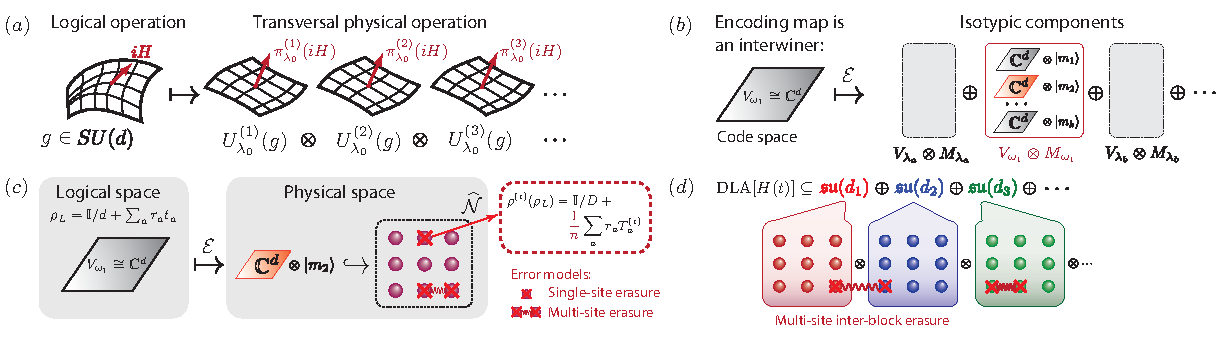
\includegraphics[width=1\linewidth]{figs/theme.pdf}
\caption{
Overview of the covariant encoding construction and its applications.
(a) Covariance relates the logical $SU(d)$ action to a physical transversal action. The logical generator $iH$ is represented physically as a sum of local generators acting on the $n$ physical subsystems, each carrying the same single-site representation $\lambda_0$.
(b) The encoding isometry embeds the logical space $V_{\omega_1}\cong\mathbb C^d$ into the physical Hilbert space. After decomposing the physical space into isotypic components $V_\lambda\otimes M_\lambda$, covariance forces the code to lie inside the component $V_{\omega_1}\otimes M_{\omega_1}$. Thus, choosing the covariant code reduces to choosing a multiplicity vector $\ket m\in M_{\omega_1}$, which selects one embedded copy of the logical representation.
(c) Error protection is analyzed through the complementary channel, which describes the information leaked to the environment. For a single-site erasure, the environment sees the reduced state $\rho^{(i)}(\rho_L)$ of the erased subsystem. In our codes, the logical-state-dependent part of this reduced state is suppressed as the number of physical subsystems grows, so the environment output becomes close to a constant channel.
(d) The same codes can be used block-wise for symmetry-constrained analog simulation. The invariant part of the dynamical Lie algebra acts transversally within each encoded block, while multi-site erasures, including erasures involving different blocks, are treated using the same reduced-state and complementary-channel method.
}
\label{fig:theme}

\end{figure*}

\let\oldaddcontentsline\addcontentsline
\renewcommand{\addcontentsline}[3]{}

\section{Introduction}\label{sec:main_intro}

Digital quantum computing has made substantial progress. Programmable processors have reached regimes that are hard to simulate classically, with growing evidence for useful pre-fault-tolerant computations in specific settings~\cite{Arute2019,Kim2023}. These experiments do not yet use full quantum error correction, but digital quantum computing has a clear fault-tolerance paradigm: encode logical qubits into many physical qubits, extract error information and correct errors repeatedly, and implement protected logical gates. Although the overheads remain large~\cite{Fowler2019, Gidney2021}, the conceptual route to long fault-tolerant digital algorithms is in place. Analog platforms offer a complementary route to quantum simulation and computation~\cite{Bloch2012,Browaeys2020,Daley2022,Schaefer2020}, with recent experiments preparing strongly correlated states, including Fermi-Hubbard systems, in regimes challenging for classical methods~\cite{Xu2025,Mazurenko2017,Shao2024,Chalopin2024}. More generally, analog devices implement continuously generated Hamiltonian dynamics, and universal analog computation can be formulated by asking whether the available Hamiltonians generate a sufficiently large dynamical Lie algebra (DLA)~\cite{Tavis1968,DAlessandro2021,Chen2020,Albertini2018,Albertini2020,Wang2016,Wang2012,Zanardi2004,AlbertiniDAlessandro2025,Hu2025}. The promise of analog computation is therefore clear, but the corresponding framework for protecting native continuous-time dynamics is much less developed than in the digital circuit model.

Noise control is central in both settings. Digital fault tolerance is supported by a mature theory and by rapid experimental progress in logical memories and small logical processors, including break-even demonstrations where increasing the number of physical qubits reduces logical error rates~\cite{Krinner2022,AcharyaGoogle2025,RyanAnderson2021,daSilvaPaetznick2024,Reichardt2024Tesseract,Bluvstein2024,Reichardt2024NeutralAtom}. For analog simulation, one can in principle digitize the target evolution and run it in a protected circuit, but this replaces continuous Hamiltonian evolution by long gate sequences and adds Trotterization or phase-estimation costs to the fault-tolerance overhead~\cite{Reiher2017ReactionMechanisms,Kivlichan2020Trotter}. This motivates noise-control strategies that are native to analog dynamics. Recent work has identified noise-stable regimes with quantum advantage~\cite{Trivedi2024AnalogStability}, provided accuracy and hardness guarantees for noisy open-system simulations~\cite{Kashyap2025AnalogOpenSimulation}, and proposed direct error-reduction methods based on Hamiltonian reshaping or rescaling~\cite{Guo2025HamiltonianReshaping}, penalty-Hamiltonian encodings~\cite{Cao2024RobustAnalog}, and continuous syndrome monitoring with feedback~\cite{Atalaya2021ContinuousQEC}. These ideas show that analog noise control need not simply reproduce digital fault tolerance. What is still missing is a general encoding principle that suppresses local noise while preserving the continuous encoded dynamics that make analog platforms natural.

A fundamental obstruction is the Eastin--Knill theorem~\cite{Eastin2009}. In an encoded analog device, the natural fault-tolerant way to implement a continuous logical operation is to realize its generator transversally, as a sum of local physical generators across the code block. Equivalently, the desired logical dynamics can be viewed as a continuous group of logical transformations, and a transversal implementation realizes the same group on the physical subsystems by a product action. In this sense, the transversal implementation defines a continuous symmetry of the encoded system: applying the group action before encoding should be equivalent to encoding first and then applying the corresponding physical action. This is the \textit{covariance} condition. However, exact finite-dimensional quantum error-correcting codes that correct local errors cannot support nontrivial continuous transversal symmetries, as stated in the Eastin--Knill theorem~\cite{Eastin2009}. Thus continuous analog dynamics and exact transversal quantum error correction are in tension. One can relax this obstruction by using infinite-dimensional covariant codes~\cite{Hayden2021}, by keeping exact finite-dimensional codes while restricting the correctable errors~\cite{Gupta2024}, or by allowing a controlled recovery error, leading to approximate quantum error correction (AQEC)~\cite{schumacher2002approximate, Beny2010}. We follow the third route: finite-dimensional covariant codes with approximate correctability.

Covariant codes can support continuous groups of transversal logical operations at the cost of controlled approximation error~\cite{Faist2020}. Quantitative trade-offs between covariance and correctability are now known, including information-theoretic lower bounds for covariant codes under erasure noise~\cite{Faist2020,Zhou2021,Faist2023,Kong2022,Yang2022}. Near-optimal scaling has been obtained from symmetric random constructions, and explicit examples have been developed for $U(1)$ covariance, W-state-type codes, and related questions in encoding complexity~\cite{Lin2025,Faist2020,Alexander2025,Yi2024}. These works establish the basic principles and limits of covariant AQEC, but many constructions are randomized, use reference frames or ancilla systems~\cite{Kong2022,Yang2022}, or address specific code families. Covariant approximate quantum error-correcting codes (AQECCs) are also relevant beyond computation. They model the protection of quantum information carrying a physical symmetry charge; they arise naturally in holographic quantum error correction and in discussions of approximate global symmetries in quantum gravity~\cite{Almheiri2015,Pastawski2015,HarlowOoguri2019}; and they are closely connected to quantum reference frames and metrology, where the same constraints can be expressed through reference-frame accuracy or quantum Fisher information~\cite{Hayden2021,Woods2020,Kubica2021}. Explicit non-Abelian covariant AQECCs therefore provide concrete models for studying how symmetry, locality, and approximate correctability can coexist.

Taken together, these developments suggest covariant AQEC as a possible route toward fault-tolerant analog quantum computation. The goal is not to digitize the dynamics into a long protected circuit, but to choose an encoded subspace that supports the relevant continuous evolution while suppressing the information leaked by local noise. Approximate correctability is essential: it allows one to evade the finite-dimensional Eastin--Knill obstruction while retaining transversal implementations of continuous symmetry generators. At the same time, covariant AQEC is not only a tool for analog computation; its capabilities and limitations are important more broadly because they clarify how symmetry, locality, and error correction can coexist, and may guide symmetry-compatible techniques for fault-tolerant quantum computation. Despite recent progress, explicit and flexible constructions remain limited. Many existing approaches focus on Abelian or otherwise restricted symmetries, randomized constructions, or single-site noise models. In many physical settings, however, one expects non-Abelian symmetries and errors that can affect several subsystems or have a more general local structure. This motivates the central question of this work: can one construct finite-dimensional covariant AQECCs for non-Abelian symmetries, such as $SU(d)$, with controllable performance under general multi-qudit noise models?

We answer this question positively. As summarized in Section~\ref{sec:main_summary}, we construct explicit finite-dimensional $SU(d)$-covariant AQECCs in which the logical system transforms as the fundamental representation and the physical system consists of many local $SU(d)$ degrees of freedom. The main idea is to use the freedom available inside the physical representation space to impose permutation symmetries on the code. These symmetries spread the logical information nearly uniformly across the physical subsystems, so that the reduced states seen by local noise depend only weakly on the logical input. We first illustrate this mechanism for $SU(2)$ in Section~\ref{sec:main_su2}, and then develop the general $SU(d)$ construction in Section~\ref{sec:main_sud}. This gives near-optimal $\Theta(1/n)$ worst-case purified-distance scaling for one-, two-, and three-qudit flagged erasures, matching known covariant-code lower bounds up to constants~\cite{Faist2020,Zhou2021}. The same reduced-state method also gives general $O(n^{-1/2})$ bounds for arbitrary flagged local noise. For single-qudit erasure, we additionally give an explicit near-optimal decoder based on the Petz recovery map~\cite{Petz1988,Barnum2002,Ng2010}. We then use these codes as block-wise building blocks for analog quantum simulation in Section~\ref{sec:main_covar_analog}: symmetry-preserving Hamiltonians act transversally within encoded invariant blocks, while the same $1/n$ protection persists for the two-qudit erasure models analyzed here, including erasures involving different blocks. Finally, in Section~\ref{sec:main_univ_analog}, we explain how controlled symmetry-breaking Hamiltonians can be used as non-transversal resource operations to enlarge the protected symmetry-preserving dynamics to universal analog control.

\section{Summary of Main Results}\label{sec:main_summary}
 
The following sections derive the main results using a representation-theoretical framework. This section summarizes them with minimal use of that formalism, for readers interested in the formulas and bounds rather than the derivations. The subsections are presented in the same order as the corresponding sections of the paper.
 
\subsection{Approximate error correction framework}\label{subsec:summary_framework}
 
A code is an isometry $V$ embedding of a small logical Hilbert space $\mathcal H_L$ into a large physical Hilbert space $\mathcal H_P=A_1\otimes\cdots\otimes A_n$ of $n$ qudits, $\mathcal E(\rho_L):=V\rho_LV^\dagger$. We say the code $\varepsilon$-approximately protects against a noise channel $\mathcal N$ if some recovery channel $\mathcal R$ can undo the noise approximately,
$$
d(\mathcal R\circ\mathcal N\circ\mathcal E,\mathrm{id}_L)\le \varepsilon,
$$
where $d$ is a fidelity-based distance between channels, Eq.~\eqref{eq:distance_def}. For a family of codes indexed by $n$ (usually being the number of physical qudits), the question is how fast $\varepsilon$ shrinks as $n$ grows. The main noise model is erasure at known locations: with probability $p_S$, the qudits in a set $S$ are discarded and replaced by a blank state, with a flag recording which qudits were lost, Eq.~\eqref{eq:erasure_noise}; we also treat the more general case of an arbitrary, possibly unknown error acting on a known set of qudits, Eq.~\eqref{eq:arbitrary_multiqudit_noise}.
 
A convenient way to think about correctability, due to \citet{Beny2010}, is to ask what an environment having access only to the discarded qudits could learn about the logical state. If that environment's state is essentially the same no matter what was encoded, the logical information was never really leaked, and a good recovery map is guaranteed to exist, Eq.~\eqref{eq:beny}. The relevant object is therefore the reduced state of the encoded qudits seen by this observer,
$$
\rho^{(S)}(\rho_L):=\operatorname{Tr}_{\bar S}\!\left(V\rho_LV^\dagger\right),
$$
and most of the technical work in the paper is a calculation of $\rho^{(S)}(\rho_L)$ for small sets $S$ of one, two, or three qudits, followed by an estimate of how strongly it depends on $\rho_L$.
 
The approximate codes we build are also required to satisfy a precise covariance condition with respect to a continuous symmetry $SU(d)$ (or a product of such groups). Let $U_L(g)$ denote the action of $g\in SU(d)$ on the logical space, and let $U_P(g)$ denote the transversal physical action obtained by applying one fixed local rotation to every qudit at once, Eq.~\eqref{eq:group_phys_space_rep}. Covariance means that the encoding isometry $V$ satisfies
$$
VU_L(g)=U_P(g)V,\qquad \forall g\in SU(d),
$$
Eq.~\eqref{eq:group_covar_cond}: rotating the logical state and then encoding it gives exactly the same physical state as encoding it first and then rotating every qudit transversally. Thus, an approximate quantum error-correcting code satisfying the covariance condition provides a code space on which the logical $SU(d)$ symmetry is implemented by continuous transversal physical operations.

Equation~\eqref{eq:group_covar_cond} is a strong constraint: it forces $V$ to map the logical space onto one specific copy of itself sitting inside the physical Hilbert space, among the several equivalent copies that occur there once $n$ is large enough. What this constraint does not fix is \emph{which} copy to choose when more than one is available, and this is exactly the freedom we exploit. We pick the copy so that it is also left invariant by permuting the physical qudits, which forces the logical information to be shared equally among them; an asymmetric choice, by contrast, is exactly what would let a handful of erased qudits give away a disproportionate share of the logical information.
 
\subsection{A first example: one logical qubit shared among many spins}\label{subsec:summary_su2}
 
The simplest version of the construction encodes a logical spin-$\tfrac12$ qubit into $n$ physical spin-$j$ systems ($n$ odd, $j$ half-integer), with logical $SU(2)$ rotations implemented as the total spin $J_a=\sum_k J_a^{(k)}, a=x, y, z$. Requiring the code to be invariant under cyclic permutations of the $n$ spins forces the logical information to be shared exactly equally among them. The reduced state of any single spin is then
$$
\rho^{(i)}(\rho_L)=\frac{I_{2j+1}}{2j+1}+\frac{3}{2nj(j+1)(2j+1)}\sum_a r_aJ_a^{(i)},
$$
for $\rho_L=\tfrac12(I+\mathbf r\cdot\boldsymbol\sigma)$. The first term, maximally mixed, carries no information about $\rho_L$; the second term, which does, is suppressed by $1/n$. Translating this into a recovery bound for flagged single-spin erasure gives
$$
d(\mathcal R\mathcal N\mathcal E,\mathrm{id})\le \frac{3}{4\sqrt{2j(j+1)}}\,\frac1n+O(n^{-2}).
$$
Known lower bounds for any $SU(2)$-covariant code under erasure scale the same way in $n$~\cite{Faist2020}, so this code is near-optimal in its $n$-scaling.
 
\subsection{The general \texorpdfstring{$SU(d)$}{SU(d)} code, a decoder, and general noise}\label{subsec:summary_sud}
 
The same mechanism works for a $d$-dimensional logical system encoded into $n$ copies of a fixed local representation of $SU(d)$ (each physical qudit carries an antisymmetric tensor power $V_{\omega_r}=\bigwedge^r\mathbb C^d$ of the fundamental representation, with generators acting as $T_a^{(i)}$; Eq.~\eqref{eq:su_d_gens}). The cyclically symmetric code again gives a one-qudit reduced state of "maximally mixed plus a $1/n$-suppressed, logical-dependent piece,"
$$
\rho^{(i)}(\rho_L)=\frac{I_{V_{\omega_r}}}{\dim V_{\omega_r}}+\frac{1}{2\kappa_{\omega_r}n}\sum_a r_aT_a^{(i)},\quad \kappa_{\omega_r}=\frac12\binom{d-2}{r-1},
$$
and a single-qudit erasure bound
$$
d(\mathcal R\mathcal N\mathcal E,\mathrm{id})\le \frac{d-1}{2\sqrt2}\sqrt{\frac{d+1}{r(d-r)}}\,\frac1n+O(n^{-2}),
$$
which again matches the known $SU(d)$ lower bound~\cite{Faist2020} in its $1/n$ scaling, up to a constant depending on $d$ and $r$.
 
We then provide an explicit recovery map, the Petz (transpose) map built directly from the encoding isometry $V$, and show that it achieves the same $1/n$ scaling, though we do not pin down its optimal constant.
 
The same reduced state also controls protection against non-erasure noise. If a single qudit undergoes an arbitrary unknown local noise channel, then the environment does not see $\rho^{(i)}(\rho_L)$ directly, but only its image under the corresponding local complementary channel. Thus, all information about the logical state still passes through the one-site reduced state $\rho^{(i)}(\rho_L)$ above. Since the logical-state-dependent part of this reduced state is suppressed with $n$, the code remains approximately correctable, with the weaker scaling $O(1/\sqrt n)$. The loss from $1/n$ to $1/\sqrt n$ comes from using a fully general, but less tight, proof technique.
 
\subsection{Protecting against multi-qudit noise}\label{subsec:summary_multierasure}
 
If two or three qudits can be erased simultaneously, at unknown but flagged locations, cyclic symmetry is no longer enough: every pair, respectively every triple, of qudits must look alike to the environment. This requires the code to be invariant under a subgroup of the permutation group that can move any pair (or triple) of sites to any other pair (or triple) -- a $2$- or $3$-transitive subgroup of all permutations of the $n$ sites. Such subgroups are rare; we use the affine group $\mathrm{AGL}(1,n)$, Eq.~\eqref{eq:AGL_def}, for two-qudit erasures and the projective linear group $\mathrm{PGL}(2,n-1)$, Eq.~\eqref{eq:PGL_def}, for three-qudit erasures, both of which admit the needed invariant codes once $n$ (respectively $n-1$) is a suitable prime power. (The full permutation group $S_n$ would also work in principle, but it is too restrictive.)
 
With this extra symmetry, the three-qudit reduced state splits into a logical-independent piece and a logical-dependent piece of size $\Theta(1/n)$, $\rho^{(ijk)}(\rho_L)=\tau^{(ijk)}+\Delta^{(ijk)}(\rho_L)$, Eq.~\eqref{eq:3q_reduced_state}, and the resulting bound for flagged three-qudit erasure is
$$
d(\mathcal R\mathcal N\mathcal E,\mathrm{id})\le \frac{\sqrt{3(d^2-1)}}{2\sqrt2}\,\frac1n+O(n^{-2}).
$$
As in the single-qudit case, the same reduced state controls protection against arbitrary (non-erasure) noise on three known qudits, at the weaker rate $O(1/\sqrt n)$.
 
\subsection{Using these codes to protect analog quantum dynamics}\label{subsec:summary_analog}
 
We also use this machinery to protect continuous-time ("analog") quantum simulation under a symmetry. If the Hamiltonians driving an analog simulator are invariant under some finite group $G$ of qubit permutations, every reachable evolution is confined to a block-diagonal "invariant algebra"
$$
\mathfrak{su}(\mathcal H)^G\cong \mathfrak{su}(d_1)\oplus\cdots\oplus\mathfrak{su}(d_k)\oplus\mathfrak u(1)^{\oplus(r-1)},
$$
Eq.~\eqref{eq:inv_alg_decomp}, where the block sizes $d_i$ are fixed by $G$ and are typically far smaller than the full Hilbert-space dimension. We then build a \emph{block encoding}, Eq.~\eqref{eq:block_enc_def}: each non-Abelian block $\mathfrak{su}(d_i)$ is encoded separately, using one of the $SU(d_i)$-covariant codes above, so that every symmetry-respecting Hamiltonian acts transversally, block by block, on the encoded system.
 
This block code still tolerates noise that mixes different blocks. For a two-block code (block sizes $n_1,n_2$) under flagged two-qudit erasure -- whether both erased qudits lie in the same block or one in each -- the recovery error again scales as
$$
d(\mathcal R\mathcal N\mathcal E,\mathrm{id})\le\frac{\sqrt{C_1(d_1^2-1)+C_2(d_2^2-1)}}{n}+O(n^{-2})
$$
for $n_1\approx n_2\approx n$, Eq.~\eqref{eq:fidelity_2}, with constants $C_1,C_2$ independent of the block dimensions. Stacking covariant codes block by block therefore preserves the same $1/n$ protection, even for erasures affecting two blocks.
 
\subsection{Towards universal analog computation}\label{subsec:summary_universal}
 
Symmetric Hamiltonians alone can only ever generate the smaller, block-diagonal invariant algebra above, which in general doesn't coincide with the full algebra needed for universal control. We give a sufficient condition, Theorem~\ref{thm:breakers_suff_cond}, under which adding a modest set of symmetry-\emph{breaking} Hamiltonians restores universality: if the resulting "coupling graph" linking the different symmetry blocks is connected, and each link is "rich enough" in a precise sense (the Full First-Factor Span condition of Appendix~\ref{sec:supple_Universal_comp}), then the symmetric Hamiltonians together with the symmetry-breaking ones generate the full algebra $\mathfrak{su}(\mathcal H)$ on the whole Hilbert space. For instance, three qubits with $S_3$ permutation symmetry become fully controllable once a single extra term, $Z_1+X_2$, is added to the symmetric Hamiltonians.
 
This suggests a possible route toward robust universal analog computation, rather than a complete architecture by itself. The block encoding protects the encoded code space, within which symmetry-preserving Hamiltonians can be implemented transversally on the corresponding covariant code blocks. Universality then requires additional symmetry-breaking Hamiltonians, which are not transversal under the block encoding and therefore act as resource operations. The usefulness of this approach depends on choosing a symmetry that gives a favorable tradeoff: the invariant block structure should reduce the required physical resources, such as the number of physical qudits or their local dimensions, while the required symmetry-breaking resource Hamiltonians should remain sufficiently simple to implement.

\section{Preliminaries}\label{sec:main_prelim}

\subsection{Approximate Quantum Error Correction}\label{subsec:main_AQEC}

We first recall the approximate error-correction framework used throughout the paper. An exact quantum error-correcting code for a given noise model is an encoding for which there exists a recovery channel that perfectly restores the logical information after the noise has acted. This requirement is too restrictive for the setting considered here. In particular, the Eastin--Knill theorem and its variants imply that finite-dimensional codes correcting local errors exactly cannot support nontrivial continuous logical symmetries transversally~\cite{Eastin2009}.

Approximate quantum error correction relaxes this condition. For a fixed noise channel, an encoding is $\varepsilon$-approximately correctable if there exists a recovery channel that reverses the noisy encoded evolution up to error at most $\varepsilon$, calculated by a chosen distance between quantum channels~\cite{Beny2010}. For an asymptotic family of codes, the central requirement is that this error decreases as the number $n$ of physical subsystems grows.

The noise model has to be specified with some care. If the noise is artificially weak, approximate correctability can arise for trivial reasons. For example, if exactly one physical qubit is erased uniformly at random among $n$ qubits, then the trivial encoding
$$
\ket\psi
\longmapsto
\ket\psi\ket 0^{\otimes(n-1)}
$$
has vanishing error as $n\to\infty$, simply because the logical qubit is erased only with probability $1/n$~\cite{Yi2024}. This does not constitute a robust error-correction mechanism. Thus, throughout the paper, we consider asymptotic code families for which the error parameter $\varepsilon$ decreases with the system size, and we work with the most general noise models for which the performance can be analyzed explicitly.

For a fixed code and noise model, one could in principle optimize over all recovery channels. This optimization is generally difficult~\cite{PhysRevA.75.012338}. We instead use the complementary-channel characterization of approximate error correction. The complementary channel describes the information leaked to the environment. Approximate correctability is equivalent to the statement that this environment output is close to independent of the logical input, or equivalently that the complementary channel is close to a constant channel, i.e., a quantum channel that maps all states to some fixed state~\cite{Beny2010, Faist2020}.

\paragraph{Correctability and distance.}

We now define the channel distance used in the paper. For two quantum channels $\mathcal N$ and $\mathcal M$, their worst-case entanglement fidelity is
$$
\begin{aligned}
&F(\mathcal N,\mathcal M)
\\
&:=
\min_\rho
f\Big(
(\mathcal N\otimes\mathrm{id})
(\ket{\psi_\rho}\bra{\psi_\rho}),
(\mathcal M\otimes\mathrm{id})
(\ket{\psi_\rho}\bra{\psi_\rho})
\Big),
\end{aligned}
$$
where $\ket{\psi_\rho}$ is a purification of $\rho$, and
$$
f(\rho,\sigma)
:=
\operatorname{Tr}
\sqrt{\sqrt\rho\sigma\sqrt\rho}
$$
is the root fidelity between states. We use the corresponding fidelity-induced channel distance
\begin{equation}\label{eq:distance_def}
d(\mathcal N,\mathcal M)
:=
\sqrt{1-F(\mathcal N,\mathcal M)} .
\end{equation}

Let
$$
\mathcal E:
\mathcal D(\mathcal H_L)
\to
\mathcal D(\mathcal H_P)
$$
be an encoding channel, where $\mathcal H_L$ and $\mathcal H_P$ are the logical and physical Hilbert spaces. For a fixed noise channel $\mathcal N$, we say that $\mathcal E$ is $\varepsilon$-correctable under $\mathcal N$~\cite{Beny2010} if there exists a recovery channel $\mathcal R$ such that
$$
d(\mathcal R\circ\mathcal N\circ\mathcal E,\mathrm{id}_L)
\le
\varepsilon .
$$

\paragraph{Flagged local noise.}

Throughout the paper, the physical Hilbert space of $n$ qudits is decomposed as
$$
\mathcal H_P
=
A_1\otimes\cdots\otimes A_n,
$$
where $A_i$ is the Hilbert space of the $i$th qudit. For a subset $S\subseteq{1,\ldots,n}$, we write
$$
A_S
:=
\bigotimes_{i\in S}A_i,
$$
and $\bar S$ denotes the complementary subset. To simplify notation, when $S={i,j,k}$, we write $A_{ijk}$, $\operatorname{Tr}_{ijk}$, $p_{ijk}$, and $\ket{ijk}$ instead of $A_S$, $\operatorname{Tr}_{A_S}$, $p_S$, and $\ket S$. Similarly, for a single site $S={i}$, we often write $i$ instead of $A_i$.

The main noise model considered in the paper is subsystem erasure at known locations, or equivalently flagged subsystem erasure. In its general form, it is
\begin{equation}\label{eq:erasure_noise}
\mathcal N(\sigma)
=
\sum_S
p_S
\ket S\bra S_F
\otimes
\ket e\bra e_{A_S}
\otimes
\operatorname{Tr}_S(\sigma),
\end{equation}
where $F$ is a classical flag register recording which subsystem $A_S$ was erased~\cite{Faist2020}. We also consider an arbitrary flagged multi-qudit noise of the form
\begin{equation}\label{eq:arbitrary_multiqudit_noise}
\mathcal N(\sigma)
=
\sum_{S\in\mathcal S}
p_S
\ket S\bra S_F
\otimes
\left(
\mathcal N_S
\otimes
\mathrm{id}_{\bar S}
\right)(\sigma),
\end{equation}
where $\mathcal N_S$ is an arbitrary noise channel acting on the subsystem $A_S=\bigotimes_{i\in S}A_i$, extending beyond erasure errors.

\paragraph{Complementary-channel criterion.}

Let
$$
\Phi:\operatorname{End}(\mathcal H_A)\to\operatorname{End}(\mathcal H_B)
$$
be a quantum channel with Stinespring dilation
$$
\Phi(\sigma)
=
\operatorname{Tr}_E(W\sigma W^\dagger),
\qquad
W:\mathcal H_A\to\mathcal H_B\otimes\mathcal H_E .
$$
The complementary channel is obtained by tracing out the channel output:
$$
\widehat\Phi(\sigma)
:=
\operatorname{Tr}_B(W\sigma W^\dagger).
$$
Thus $\Phi$ describes the system output, while $\widehat\Phi$ describes the corresponding environment output.

For a state $\rho_0$ on the environment output space, the corresponding constant channel is
\begin{equation}\label{eq:constant_channel_def}
\Lambda_0(\rho)
:=
\operatorname{Tr}(\rho)\rho_0 .
\end{equation}
The following theorem relates approximate correctability to decoupling from the environment.

\begin{theorem}[\citet{Beny2010}]\label{thm:beny}
Let $\mathcal E$ be an encoding channel, let $\mathcal N$ be a noise channel, and let $\widehat{\mathcal N\circ\mathcal E}$ be a complementary channel to $\mathcal N\circ\mathcal E$. Then
\begin{equation}\label{eq:beny}
    \min_{\mathcal R}
    d\left(
        \mathcal R\circ\mathcal N\circ\mathcal E,
        \mathrm{id}_L
    \right)
    =
    \min_{\Lambda_0\,\mathrm{constant}}
    d\left(
        \widehat{\mathcal N\circ\mathcal E},
        \Lambda_0
    \right).
\end{equation}
\end{theorem}

The theorem states that an encoding is approximately correctable precisely when the environment output can be made close to a fixed state that is independent of the logical input. This is the perspective used throughout the paper: rather than constructing a recovery map first, we control what the environment can learn.

\paragraph{Reduced states seen by the environment.}

For the erasure channel, defined in Eq.~\eqref{eq:erasure_noise}, suppose that the encoding is isometric:
\begin{equation}\label{eq:enc_isom}
\mathcal E(\rho_L)
=
V\rho_LV^\dagger .
\end{equation}
Hence, a complementary channel to the erasure channel, derived in~\cite{Faist2020}, is
\begin{equation}\label{eq:dual_to_erasure}
\widehat{\mathcal N\circ\mathcal E}(\rho_L)
=
\sum_S
p_S
\ket S\bra S_{F_E}
\otimes
\operatorname{Tr}_{\bar S}
\left(
V\rho_LV^\dagger
\right).
\end{equation}
Thus, the environment receives the erased subsystem, together with a flag recording which subsystem was erased.

For the arbitrary flagged multi-qudit noise model~\eqref{eq:arbitrary_multiqudit_noise}, let $\widehat{\mathcal N}_S$ be a complementary channel to $\mathcal N_S$. Then, as shown in Lemma~\ref{lem:dual_to_arb},
\begin{equation}\label{eq:dual_to_arbitrary_multiqudit}
\widehat{\mathcal N\circ\mathcal E}(\rho_L)
=
\sum_{S\in\mathcal S}
p_S
\ket S\bra S_{F_E}
\otimes
\widehat{\mathcal N}_S
\left(
\operatorname{Tr}_{\bar S}
\left(
V\rho_LV^\dagger
\right)
\right).
\end{equation}

Eqs.~\eqref{eq:dual_to_erasure} and~\eqref{eq:dual_to_arbitrary_multiqudit} show that local reduced states of the encoded state are the central objects in the complementary-channel analysis. We therefore use the notation
\begin{equation}\label{eq:reduced_state}
\rho^{(S)}(\rho_L)
:=
\operatorname{Tr}_{\bar S}
\left(
V\rho_LV^\dagger
\right),
\end{equation}
where $S\subseteq{1,\ldots,n}$. In particular,
$$
\rho^{(i)}(\rho_L),
\qquad
\rho^{(ij)}(\rho_L),
\qquad
\rho^{(ijk)}(\rho_L)
$$
denote the one-, two-, and three-qudit reduced states, respectively. The main calculations below are calculations of these reduced states and of how much they depend on the logical input.

\subsection{Covariant encoding}\label{subsec:main_covar_enc}

We now introduce the covariant encoding framework used throughout the paper. Approximate correctability allows us to keep continuous logical symmetries implemented locally, while relaxing exact correction to correction with a controlled error. The compatibility condition between an encoding and a symmetry is \textit{covariance}~\cite{Hayden2021}. In representation-theoretic language, covariance says that the encoding map is an \textit{intertwiner} between the logical and physical representations.

For the codes constructed below, the logical system carries the fundamental representation of $SU(d)$. Constructing a covariant code therefore amounts to embedding a copy of this representation into the physical Hilbert space. Representation theory identifies where such copies can occur, and the remaining freedom is a choice of vector in the corresponding multiplicity space~\cite{Denys2024}. We use this freedom to impose additional permutation symmetries on the code space. Specifically, we choose the multiplicity vector to be invariant under a suitable subgroup of the permutation group on $n$ elements $G_P\subseteq S_n$ acting by permutations of the physical subsystems. Since this permutation action commutes with the collective $SU(d)$ action, it acts only on multiplicity spaces. Thus a $G_P$-invariant multiplicity vector gives a $G_P$-invariant code space. The choice of $G_P$ depends on the noise model and will be specified in the later sections.

\paragraph{Covariance.}

Let $G$ be a compact connected Lie group, and let $\mathfrak g$ be its Lie algebra. Let
$$
V:\mathcal H_L\to\mathcal H_P
$$
be the encoding isometry associated with the encoding channel in Eq.~\eqref{eq:enc_isom}. Let $U_L$ and $U_P$ be unitary representations of $G$ on $\mathcal H_L$ and $\mathcal H_P$, respectively. We say that $V$ is $G$-\textit{covariant with respect to $U_L$ and $U_P$} if
\begin{equation}\label{eq:group_covar_cond}
VU_L(g)
=
U_P(g)V,
\qquad
\forall g\in G .
\end{equation}
Equivalently, let $\pi_L$ and $\pi_P$ be the corresponding Lie-algebra representations,
$$
\pi_L(X)
:=
\left.\frac{d}{dt}\right|_{t=0}
U_L(e^{tX}),
\qquad
\pi_P(X)
:=
\left.\frac{d}{dt}\right|_{t=0}
U_P(e^{tX}).
$$
Then $V$ is \textit{$\mathfrak g$-covariant with respect to $\pi_L$ and $\pi_P$} if
\begin{equation}\label{eq:algebra_covar_cond}
V\pi_L(X)
=
\pi_P(X)V,
\qquad
\forall X\in\mathfrak g .
\end{equation}
Eq.~\eqref{eq:algebra_covar_cond} follows from Eq.~\eqref{eq:group_covar_cond} by differentiation. Conversely, for a connected Lie group, Eq.~\eqref{eq:algebra_covar_cond} determines the corresponding covariance condition at the group level.

We will say that the encoding channel $\mathcal E$ is \textit{$G$-covariant}, or \textit{$\mathfrak g$-covariant}, when its encoding isometry satisfies Eq.~\eqref{eq:group_covar_cond}, or equivalently Eq.~\eqref{eq:algebra_covar_cond}. We will often specify covariance at the Lie-algebra level, because the physical representations used below are most naturally described by their infinitesimal generators. This is also the natural language in the analog-simulation setting, where the relevant algebras have the form
$$
\mathfrak{su}(d_1)
\oplus
\mathfrak{su}(d_2)
\oplus
\cdots .
$$
When the representations are clear from context, we simply say that the code is \textit{$G$-covariant}.

\paragraph{Intertwiners.}

The covariance condition strongly restricts the possible encoding maps. It is precisely the condition that $V$ is an \textit{intertwiner}. Recall that if $(\mathcal V,\rho_{\mathcal V})$ and $(\mathcal W,\rho_{\mathcal W})$ are representations of a group $G$, then a linear map $A:\mathcal V\to\mathcal W$ is a \textit{$G$-intertwiner} if
\begin{equation}\label{eq:intertwiner_def}
A\circ\rho_{\mathcal V}(g)
=
\rho_{\mathcal W}(g)\circ A,
\qquad
\forall g\in G .
\end{equation}
Here $G$ may be finite or continuous. At the Lie-algebra level, for infinitesimal representations $d\rho_{\mathcal V}$ and $d\rho_{\mathcal W}$, this condition becomes
$$
A\circ d\rho_{\mathcal V}(X)
=
d\rho_{\mathcal W}(X)\circ A,
\qquad
\forall X\in\mathfrak g .
$$

The structure of intertwiners is controlled by Schur's lemma. If $V_\lambda$ and $V_\mu$ are irreducible complex representations of $G$, then
$$
\operatorname{Hom}_G(V_\lambda,V_\mu)
=
\begin{cases}
0, & \lambda\not\simeq\mu,\\
\mathbb C\cdot I_{V_\lambda}, & \lambda\simeq\mu .
\end{cases}
$$
Thus an intertwiner cannot map an irreducible representation to an inequivalent irreducible representation; it can only map it to an equivalent copy.

More generally, suppose that two finite-dimensional $G$-representations decompose as
$$
\mathcal W
\cong
\bigoplus_{\lambda\in\Lambda}
V_\lambda\otimes M_\lambda,
\qquad
\mathcal V
\cong
\bigoplus_{\lambda\in\Lambda}
V_\lambda\otimes N_\lambda,
$$
where $\Lambda$ is the set of irreducible representations of $G$, and $M_\lambda$ and $N_\lambda$ are multiplicity spaces. Then every intertwiner $A:\mathcal W\to\mathcal V$ has the form
\begin{equation}\label{eq:intertwiner_decomp}
A
\cong
\bigoplus_{\lambda\in\Lambda}
I_{V_\lambda}\otimes A_\lambda,
\qquad
A_\lambda\in\operatorname{Hom}(M_\lambda,N_\lambda).
\end{equation}
Thus the intertwiner acts trivially on the irrep factor $V_\lambda$ and only acts nontrivially on the corresponding multiplicity spaces.

This observation will be used repeatedly. Besides the encoding isometry itself, the linear extensions of reduced-state maps and the compression map
$$
X
\longmapsto
V^\dagger X V
$$
are also intertwiners. This is why representation theory fixes much of the structure of the reduced states and compressed local operators appearing below. Throughout the paper, we use the terms covariant map and intertwiner interchangeably: the term covariant is standard in quantum information theory, especially for channels and encodings, while intertwiner is the standard representation-theoretic term.

\paragraph{The $SU(d)$ representation setting.}

The main Lie group considered in this work is $SU(d)$. Since $SU(d)$ is compact, connected, and simply connected, its irreducible representations are in one-to-one correspondence with irreducible representations of $\mathfrak{su}(d)$. We will therefore freely pass between $SU(d)$ and $\mathfrak{su}(d)$ representations. Background on these representation-theoretic facts can be found in Ref.~\cite{Hall2015}.

The physical system consists of $n$ identical subsystems, each carrying the same irreducible representation of $SU(d)$. Thus the physical Hilbert space is
\begin{equation}\label{eq:phys_space_rep}
\mathcal H_P
:=
(V_{\lambda_0})^{\otimes n},
\end{equation}
where $V_{\lambda_0}$ is a fixed irreducible representation of $SU(d)$. The transversal group action is
\begin{equation}\label{eq:group_phys_space_rep}
U_P(g)
=
\bigotimes_{i=1}^n
U_{\lambda_0}^{(i)}(g),
\qquad
g\in SU(d),
\end{equation}
where $U_{\lambda_0}^{(i)}(g)$ acts as $U_{\lambda_0}(g)$ on the $i$th tensor factor. At the Lie-algebra level, the derived representation is
\begin{equation}\label{eq:alg_phys_space_rep}
\pi_P(X)
=
\sum_{i=1}^n
\pi_{\lambda_0}^{(i)}(X),
\qquad
X\in\mathfrak{su}(d),
\end{equation}
where $\pi_{\lambda_0}^{(i)}(X)$ acts as $\pi_{\lambda_0}(X)$ on the $i$th tensor factor and as the identity on all other tensor factors. For illustration of Lie group and corresponding Lie algebra actions, see Fig.~\ref{fig:theme}(a).

The logical Hilbert space is the fundamental representation of $SU(d)$:
\begin{equation}\label{eq:log_space_rep}
\mathcal H_L
:=
V_{\omega_1}
\cong
\mathbb C^d .
\end{equation}
The notation $V_{\omega_1}$ is explained in Appendix~\ref{sec:supple_sud}. We denote the corresponding group action by
$$
U_L(g)
=
u(g),
\qquad
g\in SU(d),
$$
and the corresponding Lie-algebra representation by
$$
\pi_L(X)
=
\bar X,
\qquad
X\in\mathfrak{su}(d).
$$
The bar is used only when we want to emphasize that the generator acts on the logical fundamental representation, rather than on one of the physical tensor factors.

\paragraph{Multiplicity-vector form of the encoding.}

Decompose the physical Hilbert space into irreducible $SU(d)$-representations:
\begin{equation}\label{eq:isotipic_decomp}
(V_{\lambda_0})^{\otimes n}
\cong
\bigoplus_{\lambda\in\Lambda}
V_\lambda\otimes M_\lambda .
\end{equation}
Here $V_\lambda\otimes M_\lambda$ is the isotypic component associated with the irrep $V_\lambda$, and $M_\lambda$ is its multiplicity space~\cite{Kong2022}. Since the logical space is $V_{\omega_1}$, Eq.~\eqref{eq:intertwiner_decomp} implies that the image of any covariant encoding must lie inside the corresponding isotypic component
$$
V_{\omega_1}\otimes M_{\omega_1}
\subseteq
\mathcal H_P .
$$
Thus a covariant encoding selects one copy of $V_{\omega_1}$ inside the physical Hilbert space. Equivalently, it is specified by a \textit{multiplicity vector} $\ket{m_{\omega_1}}\in M_{\omega_1}$:
\begin{equation}\label{eq:mult_vec_enc}
V:
\mathcal H_L
\cong
V_{\omega_1}
\longrightarrow
V_{\omega_1}\otimes\ket{m_{\omega_1}}
\subseteq
\mathcal H_P;
\end{equation}
see Fig.~\ref{fig:theme}(b) for schematic illustration. The choice of $\ket{m_{\omega_1}}$ determines the particular covariant code. The same multiplicity-space viewpoint was used in Ref.~\cite{Denys2024} to reconstruct known quantum error-correcting codes covariant under finite symmetry groups.

This construction is possible only if the fundamental isotypic component is present in the physical representation, that is, only if
$$
\dim M_{\omega_1}>0 .
$$
For each explicit construction below, we will specify conditions ensuring this nonzero multiplicity.

It is useful to describe the encoding in terms of the Schur transform. For a representation $\mathcal H$ of $SU(d)$, the Schur transform is a unitary
$$
U_{\mathrm{Schur}}:
\mathcal H
\longrightarrow
\bigoplus_{\lambda\in\Lambda}
V_\lambda\otimes M_\lambda
$$
such that
\begin{equation}\label{eq:schur_transform}
U_{\mathrm{Schur}}
U(g)
U_{\mathrm{Schur}}^\dagger
=
\bigoplus_{\lambda\in\Lambda}
U_\lambda(g)\otimes I_{M_\lambda}.
\end{equation}
The Schur transform is not canonical; it depends on choices of bases in the irreducible spaces $V_\lambda$ and in the multiplicity spaces $M_\lambda$. Its construction in quantum information settings is discussed in Ref.~\cite{Bacon2006}.

With this notation, the encoding associated with the multiplicity vector $\ket{m_{\omega_1}}\in M_{\omega_1}$ is
\begin{equation}\label{eq:schur_transform_enc}
V
=
U_{\mathrm{Schur}}^\dagger
\left(
I_{V_{\omega_1}}
\otimes
\ket{m_{\omega_1}}
\right).
\end{equation}

\paragraph{Permutation symmetry of the code space.}

In addition to the $SU(d)$ action, we will use finite permutation symmetries of the physical subsystems. Let $G_P\subseteq S_n$ act on $\mathcal H_P$ by permuting tensor factors:
\begin{equation}\label{eq:group_act_on_phys_space}
P_g
\left(
\ket{i_1}\otimes\cdots\otimes\ket{i_n}
\right)
:=
\ket{i_{g^{-1}(1)}}\otimes\cdots\otimes\ket{i_{g^{-1}(n)}} .
\end{equation}
This permutation action commutes with the transversal $SU(d)$ action in Eq.~\eqref{eq:group_phys_space_rep}, because $SU(d)$ acts identically on each tensor factor. Hence $G_P$ preserves the isotypic decomposition~\eqref{eq:isotipic_decomp}. By the double-centralizer structure of the commutant, the action of $G_P$ has the form~\cite{GoodmanWallach2009}
\begin{equation}\label{eq:group_act_on_code}
P_g
=
\bigoplus_{\lambda\in\Lambda}
I_{V_\lambda}\otimes R_\lambda(g),
\end{equation}
where $R_\lambda$ is a representation of $G_P$ on the multiplicity space $M_\lambda$. Thus $G_P$ acts trivially on the $SU(d)$-irrep factor and nontrivially only on the multiplicity space.

The purpose of introducing $G_P$ is to impose an additional symmetry on the code space. After covariance fixes the relevant isotypic component, the remaining freedom is the choice of the multiplicity vector. We choose this vector from the $G_P$-invariant subspace
\begin{equation}\label{eq:g_inv_subspace}
M_{\omega_1}^{G_P}
:=
\left\{
\ket m\in M_{\omega_1}
:
R_{\omega_1}(g)\ket m=\ket m
\ \forall g\in G_P
\right\}.
\end{equation}

If $\ket m\in M_{\omega_1}^{G_P}$, then the code space
$$
V_{\omega_1}\otimes\ket m
$$
is invariant under $G_P$, because $G_P$ acts as the identity on $V_{\omega_1}$ and preserves $\ket m$ in the multiplicity space.

Finally, the same permutation action induces an action on operators by conjugation. For $X\in\operatorname{End}(\mathcal H_P)$ and $g\in G_P$, define
\begin{equation}\label{eq:group_act_oper}
g\cdot X
:=
P_gXP_g^\dagger,
\end{equation}
where $P_g$ is the permutation operator from Eq.~\eqref{eq:group_act_on_phys_space}.

\section{\texorpdfstring{$SU(2)$}{SU(2)}-covariant Approximate Quantum Error Correction Codes}\label{sec:main_su2}

We begin the explicit construction with the familiar case of $SU(2)$. The logical system is a spin-$1/2$ degree of freedom, while the physical system consists of many spin-$j$ subsystems. Covariance fixes the symmetry sector in which the code can live, but it still leaves a multiplicity-space freedom. We use this remaining freedom to distribute the logical spin uniformly over the physical sites. For single-site erasure, this is precisely the relevant design principle: the environment receives a one-site reduced state, and the code is good when this reduced state is nearly independent of the logical input.

%\subsection{\texorpdfstring{Setup and reduced-state strategy}{Setup and reduced-state strategy}}
\paragraph{Setup and reduced-state strategy.}

Let $V_j$ denote the irreducible spin-$j$ representation of $SU(2)$. We take the logical Hilbert space~\eqref{eq:log_space_rep} to be
\[
    \mathcal H_L = V_{1/2}\cong \mathbb C^2,
\]
and the physical Hilbert space~\eqref{eq:phys_space_rep} to be
\[
    \mathcal H_P = (V_j)^{\otimes n},
\]
where $n$ is odd and $j\in \frac12+\mathbb Z$ is half-integer. These conditions are exactly those ensuring that the spin-$1/2$ representation appears in $(V_j)^{\otimes n}$, or equivalently that the multiplicity space $M_{V_{1/2}}$ is nonzero:
\[
    \dim M_{V_{1/2}}>0
    \quad\Longleftrightarrow\quad
    n\equiv 1 \pmod 2
    \quad\text{and}\quad
    j\in \frac12+\mathbb Z .
\]
We use the standard spin-operator notation for the physical representation~\eqref{eq:alg_phys_space_rep} of the generators of $\mathfrak{su}(2)$,
\[
    \pi_j^{(k)}\left(\frac{i\sigma_a}{2}\right)
    \equiv J_a^{(k)},
    \qquad a=x,y,z,
\]
so that the transversal physical action is
\begin{equation}\label{eq:su2_cov_rep}
    \frac{i\sigma_a}{2}
    \longmapsto
    iJ_a
    :=
    \sum_{k=1}^n iJ_a^{(k)},
    \qquad a=x,y,z .
\end{equation}

This $SU(2)$ setting is useful both as a physically transparent example and as a complete illustration of the general method. The main object is the one-site reduced state $\rho^{(i)}(\rho_L)$ defined in Eq.~\eqref{eq:reduced_state}. For flagged single-qudit erasure, this is precisely the state received by the environment, as follows from the complementary channel in Eq.~\eqref{eq:dual_to_erasure}. Thus the task is to choose the code so that $\rho^{(i)}(\rho_L)$ approaches a fixed state, independent of $\rho_L$, as $n$ grows. A detailed derivation of the final expression~\eqref{eq:reduced_state_su2} is given in Proposition~\ref{prop:SU2cov}; here we spell out the representation-theoretic mechanism.

\paragraph{Reduced-state structure from covariance.}
The form of $\rho^{(i)}(\rho_L)$ is strongly constrained by covariance. It satisfies
\begin{equation}\label{eq:reduced-state_cov_cond}
    \rho^{(i)}\!\left(u(g)\rho_Lu(g)^\dagger\right)
    =
    U_j^{(i)}(g)\rho^{(i)}(\rho_L)\bigl(U_j^{(i)}(g)\bigr)^\dagger .
\end{equation}
Equivalently, after extending $\rho^{(i)}$ linearly from density matrices to all operators on the logical space, the resulting map
\[
    \operatorname{End}(V_{1/2})
    \xrightarrow{\;\Phi^{(i)}\;}
    \operatorname{End}(V_j)
\]
is an $SU(2)$-intertwiner~\eqref{eq:intertwiner_def}, where both operator spaces carry the adjoint action. We can therefore determine its possible form from representation theory. On the logical space,
\[
    \operatorname{End}(V_{1/2})
    \cong
    V_{1/2}\otimes V_{1/2}^*
    \cong
    V_0\oplus V_1,
\]
where $V_0$ is the trivial representation, spanned by the identity, and $V_1$ is the adjoint representation, spanned by the Pauli generators. On a physical spin-$j$ site,
\[
    \operatorname{End}(V_j)
    \cong
    V_j\otimes V_j^*
    \cong
    \bigoplus_{\ell=0}^{2j} V_\ell .
\]
Thus Eq.~\eqref{eq:intertwiner_decomp} implies that $\Phi^{(i)}$ maps the trivial component of $\operatorname{End}(V_{1/2})$ to the unique trivial component of $\operatorname{End}(V_j)$, and maps the adjoint component of $\operatorname{End}(V_{1/2})$ to the unique adjoint component of $\operatorname{End}(V_j)$.

Writing the logical state in Bloch form,
\[
    \rho_L=\frac12(I+\mathbf r\cdot\boldsymbol\sigma),
\]
the identity term belongs to the trivial representation and therefore maps to a multiple of the identity on $V_j$. Normalization fixes this multiple to be $1/(2j+1)$. The traceless term belongs to the adjoint representation, and hence its image must be proportional to the unique adjoint component on $\operatorname{End}(V_j)$, spanned by the physical spin operators $J_a^{(i)}$. Therefore the reduced state has the form
\begin{equation}\label{eq:reduced_state_beta}
    \rho^{(i)}(\rho_L)
    =
    \frac{I_{2j+1}}{2j+1}
    +
    \beta^{(i)}
    \sum_{a=x,y,z} r_a J_a^{(i)} .
\end{equation}
At this stage the code space has not yet been specified; all dependence on the multiplicity vector~\eqref{eq:mult_vec_enc} is contained in the scalar coefficients $\beta^{(i)}$.

To determine these coefficients, we first compress local spin operators to the code space. Since the encoding is covariant, the total physical spin acts as the logical spin,
\begin{equation}\label{eq:total_spin_act}
    V^\dagger \sum_{i=1}^n J_a^{(i)} V
    =
    \frac{\sigma_a}{2} .
\end{equation}
Moreover, the compression map $X\mapsto V^\dagger X V$ is again an $SU(2)$-intertwiner $\operatorname{End}(V_j)\rightarrow \operatorname{End}(V_{1/2})$. Since the operators $J_a^{(i)}$ span an adjoint component on the $i$th site, Eq.~\eqref{eq:intertwiner_decomp} implies that their compression must be proportional to the unique adjoint component on the logical spin-$1/2$ space. Hence
\begin{equation}\label{eq:alpha_def}
    V^\dagger J_a^{(i)} V
    =
    \alpha^{(i)}\frac{\sigma_a}{2},
\end{equation}
for real scalars $\alpha^{(i)}$ satisfying $\sum_i\alpha^{(i)}=1$, where the latter identity follows from Eq.~\eqref{eq:total_spin_act}. Comparing Hilbert--Schmidt inner products in Eqs.~\eqref{eq:reduced_state_beta} and~\eqref{eq:alpha_def} gives
\begin{equation}\label{eq:beta_through_alpha}
    \beta^{(i)}
    =
    \frac{3\alpha^{(i)}}{2j(j+1)(2j+1)} .
\end{equation}

\paragraph{Cyclic invariance.}

It remains to choose the multiplicity vector so that the coefficients $\alpha^{(i)}$ are uniform. We do this by choosing $\ket m$ to be an eigenvector of the cyclic shift $s\in C_n\subseteq S_n$. Equivalently, the code space is invariant under cyclic permutations of the physical qudits. If $P_s$ denotes the corresponding permutation operator, then $P_s J_a^{(i)}P_s^\dagger=J_a^{(i+1)}$, while on the code space $P_sV=e^{i\phi}V$. Therefore
\[
    V^\dagger J_a^{(i+1)}V
    =
    V^\dagger P_sJ_a^{(i)}P_s^\dagger V
    =
    V^\dagger J_a^{(i)}V .
\]
All coefficients $\alpha^{(i)}$ are equal. Since they sum to one, $\alpha^{(i)}=1/n$ for every site.

For the cyclically invariant $SU(2)$-covariant code, the one-site reduced state is therefore
\begin{equation}\label{eq:reduced_state_su2}
    \rho^{(i)}(\rho_L)
    =
    \frac{I_{2j+1}}{2j+1}
    +
    \frac{3}{2nj(j+1)(2j+1)}
    \sum_{a=x,y,z} r_a J_a^{(i)},
\end{equation}
where $i=1,\ldots,n$ and $\rho_L=\frac12(I+\mathbf r\cdot\boldsymbol\sigma)$. This expression makes the error-correction mechanism transparent: the logical-state-dependent part of the erased site's density matrix is suppressed by $1/n$, so the environment's state approaches the maximally mixed state as $n$ grows.

\paragraph{Single-site erasure bound.}
We now translate this reduced-state statement into an AQEC bound. Since all one-site reduced states are identical up to the natural identification of the physical sites, the complementary channel for flagged single-site erasure becomes
\begin{equation}\label{eq:comp_chan_su2}
    \widehat{\mathcal N\circ\mathcal E}(\rho_L)
    =
    \sum_i p_i\ket i\!\bra i_{F_E}\otimes \rho^{(i)}(\rho_L)
    \cong
    \omega_{\mathrm{flag}}\otimes \rho^{(1)}(\rho_L),
\end{equation}
where
\[
    \omega_{\mathrm{flag}}
    :=
    \sum_i p_i\ket i\!\bra i_{F_E} .
\]
We compare this channel with the constant channel
\[
    \Lambda_0(\rho)
    :=
    \operatorname{Tr}(\rho)\,
    \omega_{\mathrm{flag}}\otimes \frac{I_{2j+1}}{2j+1} .
\]
The explicit fidelity calculation, given in Proposition~\ref{prop:SU2covFidelity}, yields
\begin{equation}\label{eq:fidelity_su2}
    F\!\left(\widehat{\mathcal N\circ\mathcal E},\Lambda_0\right)
    =
    1-
    \frac{9}{32n^2j(j+1)}
    +O(n^{-3}) .
\end{equation}
Together with the complementary-channel characterization of AQEC, this yields the following result.

\begin{theorem}\label{thrm:su2scale}
Let $\mathcal H_L=V_{1/2}$ and $\mathcal H_P=(V_j)^{\otimes n}$, with $n$ odd and $j\in\frac12+\mathbb Z$. Equip $\mathcal H_L$ with the fundamental spin-$1/2$ representation of $\mathfrak{su}(2)$ and $\mathcal H_P$ with the transversal spin-$j$ representation
\begin{equation}
    \frac{i\sigma_a}{2}
    \longmapsto
    iJ_a
    \equiv
    \sum_{k=1}^n iJ_a^{(k)},
    \qquad a=x,y,z .
\end{equation}
Let $\mathcal E$ be an $\mathfrak{su}(2)$-covariant encoding whose code space is invariant under cyclic permutations of the physical qudits. Then, for the flagged single-qudit erasure channel
\[
    \mathcal N(\sigma)
    =
    \sum_{i=1}^n p_i\ket i\!\bra i_F
    \otimes \ket e\!\bra e_{A_i}
    \otimes \operatorname{Tr}_i(\sigma),
\]
there exists a recovery channel $\mathcal R$ such that
\[
    d(\mathcal R\mathcal N\mathcal E,\mathrm{id})
    \le
    \frac{3}{4\sqrt{2j(j+1)}}\frac{1}{n}
    +O(n^{-2}) .
\]
In particular, the code is $O\!\left(1/(\sqrt{j(j+1)}\,n)\right)$-correctable against flagged single-qudit erasure.
\end{theorem}

\begin{proof}
By Eq.~\eqref{eq:fidelity_su2} and the definition of the channel distance in Eq.~\eqref{eq:distance_def},
\[
    d\!\left(\widehat{\mathcal N\circ\mathcal E},\Lambda_0\right)
    =
    \frac{3}{4\sqrt{2j(j+1)}}\frac{1}{n}
    +O(n^{-2}) .
\]
The complementary-channel theorem, Eq.~\eqref{eq:beny}, gives
\[
    \min_{\mathcal R}
    d(\mathcal R\mathcal N\mathcal E,\mathrm{id})
    =
    \min_{\Lambda\,\mathrm{constant}}
    d\!\left(\widehat{\mathcal N\circ\mathcal E},\Lambda\right)
    \le
    d\!\left(\widehat{\mathcal N\circ\mathcal E},\Lambda_0\right),
\]
and the stated bound follows.
\end{proof}

Known lower bounds for covariant codes under erasure noise~\cite{Faist2020} give
\[
    \min_{\mathcal R}
    d(\mathcal R\mathcal N\mathcal E,\mathrm{id})
    \ge
    \frac{1}{4\sqrt{2}\,j}\frac{1}{n} .
\]
Thus the construction is optimal in its scaling with $n$ and $j$, up to constant factors.


\section{\texorpdfstring{$SU(d)$}{SU(d)}-covariant Approximate Quantum Error Correction Codes}\label{sec:main_sud}

We now extend the construction to $SU(d)$. The logical system carries the fundamental representation, while each physical subsystem carries an antisymmetric tensor-power representation. As in the $SU(2)$ case, covariance fixes the symmetry sector in which the code can live, but leaves a freedom in the corresponding multiplicity space. We use this freedom to choose a code space that is invariant under suitable permutations of the physical subsystems. For single-qudit flagged erasure, cyclic permutation symmetry is sufficient: it spreads the logical information uniformly over the physical sites, so that each erased-site reduced state becomes nearly independent of the logical input.

\paragraph{Single-site physical representation.}

We first define the single-site physical representation. For $1\le r\le d-1$, let
\begin{equation}\label{eq:vomegar_def}
V_{\omega_r}:=\bigwedge^r \mathbb C^d .
\end{equation}
This space has basis vectors
$$
e_I:=e_{i_1}\wedge\cdots\wedge e_{i_r},
\qquad
1\le i_1<\cdots<i_r\le d,
$$
where $\wedge$ denotes the wedge product. Its dimension is
$$
\dim V_{\omega_r}=\binom{d}{r}.
$$
The action of $X\in\mathfrak{su}(d)$ on $V_{\omega_r}$ is defined by
\begin{equation}\label{eq:sud_vomegar_def}
\pi_{\omega_r}(X)
\left(v_1\wedge\cdots\wedge v_r\right)
:=
\sum_{m=1}^r
v_1\wedge\cdots\wedge Xv_m\wedge\cdots\wedge v_r .
\end{equation}
This is an irreducible representation; see Ref.~\cite{FultonHarris1991}. The notation $V_{\omega_r}$ is explained in Appendix~\ref{sec:supple_sud}.

We use the standard generators of the fundamental representation of $\mathfrak{su}(d)$. Let ${t_a}_{a=1}^{d^2-1}$ be traceless Hermitian $d\times d$ matrices satisfying
\begin{equation}
t_a t_b
=
\frac{1}{2d}\delta_{ab}I_d
+
\frac12
\sum_{c=1}^{d^2-1}
\left(i f_{abc}+d_{abc}\right)t_c ,
\end{equation}
where $f_{abc}$ are completely antisymmetric structure constants and $d_{abc}$ are completely symmetric coefficients. Further properties of these generators are collected in Appendix~\ref{sec:supple_sud}.

We take the logical Hilbert space~\eqref{eq:log_space_rep} to be the fundamental representation
$$
\mathcal H_L:=V_{\omega_1}\cong \mathbb C^d ,
$$
and the physical Hilbert space~\eqref{eq:phys_space_rep} to be
$$
\mathcal H_P:=(V_{\omega_r})^{\otimes n},
$$
where $r\neq 0,d$ and $nr\equiv 1\pmod d$. We denote the action of the generator $t_a$ on the $j$th physical subsystem by
\begin{equation}\label{eq:su_d_gens}
    \pi_{\omega_r}^{(j)}(t_a)\equiv T_a^{(j)},
    \qquad
    a=1,\ldots,d^2-1 .
\end{equation}

Thus the transversal physical representation~\eqref{eq:alg_phys_space_rep} is specified on generators by
$$
t_a
\longmapsto
T_a
:=
\sum_{i=1}^n T_a^{(i)},
\qquad
a=1,\ldots,d^2-1 .
$$
In this section the representation $V_{\omega_r}$ is fixed, so we omit the subscript $\omega_r$ from the local generators. In later sections and in the main theorems, we will often specify the physical representation by giving the images of the Lie-algebra generators.

The condition $nr\equiv 1\pmod d$ ensures that $\mathcal H_P$ contains a copy of the fundamental representation. Equivalently, the $V_{\omega_1}$-isotypic component is nonzero, so it can contain the image of an $SU(d)$-covariant encoding of the logical space. Lemma~\ref{lem:fundamental_in_extirior_power} proves that this condition is sufficient for $(V_{\omega_r})^{\otimes n}$ to contain $V_{\omega_1}$. It is not necessary in general; for example, the $SU(2)$ construction in Section~\ref{sec:main_su2} used arbitrary half-integer spin-$j$ irreducible representations as physical subsystems.

\paragraph{One-site reduced state.}

The main object is again the one-site reduced state $\rho^{(i)}(\rho_L)$ defined in Eq.~\eqref{eq:reduced_state}. A detailed derivation of its final form is given in Proposition~\ref{prop:SUdcov}. Here we describe the representation-theoretic structure of the calculation.

Write the logical state in the generalized Bloch form
\begin{equation}\label{eq:general_bloch}
\rho_L
=
\frac{I}{d}
+
\left(\rho_L-\frac{I}{d}\right)
=
\frac{I}{d}
+
\sum_a r_a t_a .
\end{equation}
The reduced-state map extends linearly to a map
$$
    \operatorname{End}(V_{\omega_1})
    \xrightarrow{\;\Phi^{(i)}\;}
    \operatorname{End}(V_{\omega_r}) .
$$
By covariance, this map is an $SU(d)$-intertwiner~\eqref{eq:intertwiner_def}, where both operator spaces carry the adjoint action. As shown in Lemma~\ref{lem:adjoint_in_end}, $\operatorname{End}(V_{\omega_r})$ contains unique copies of both the trivial representation and the adjoint representation. Therefore, using the intertwiner decomposition~\eqref{eq:intertwiner_decomp}, the identity component of $\operatorname{End}(V_{\omega_1})$ must map to the identity component of $\operatorname{End}(V_{\omega_r})$, while the adjoint component must map to the adjoint component. Hence
\begin{equation}\label{eq:linear_ext_of_red_state}
\begin{gathered}
\Phi^{(i)}\left(\frac{I_d}{d}\right)
=
\frac{I_{V_{\omega_r}}}{\dim V_{\omega_r}},
\\
\Phi^{(i)}\left(\sum_a r_a t_a\right)
=
\beta^{(i)}
\sum_a r_a T_a^{(i)} .
\end{gathered}
\end{equation}
Thus the reduced state has the form
\begin{equation}\label{eq:reduced_state_sud}
\rho^{(i)}(\rho_L)
=
\frac{I_{V_{\omega_r}}}{\dim V_{\omega_r}}
+
\beta^{(i)}
\sum_a r_a T_a^{(i)}.
\end{equation}

The coefficients $\beta^{(i)}$ are determined by the compression of local generators to the code space. Since the encoding is covariant, the total physical action restricts to the logical fundamental action. For each local generator, the compression map $X\mapsto V^\dagger X V$ is again an $SU(d)$-intertwiner $\operatorname{End}(V_{\omega_r})\rightarrow \operatorname{End}(V_{\omega_1})$, and therefore
$$
V^\dagger T_a^{(i)}V
=
\alpha^{(i)}\bar t_a ,
$$
where
$$
\sum_i\alpha^{(i)}=1,
$$
and $\bar t_a$ denotes the fundamental generator acting on the logical space. The relation between $\alpha^{(i)}$ and $\beta^{(i)}$ is obtained by comparing Hilbert--Schmidt inner products, exactly as in the $SU(2)$ case, giving
$$
\beta^{(i)}
=
\frac{\alpha^{(i)}}{2\kappa_{\omega_r}},
\qquad
\kappa_{\omega_r}
=
\frac12\binom{d-2}{r-1}.
$$

It remains to choose the multiplicity vector. We choose $\ket m$ to be an eigenvector of the cyclic shift operator. Equivalently, the code space $V_{\omega_1}\otimes\ket m$ is invariant under cyclic permutations of the physical qudits. The same argument as in Section~\ref{sec:main_su2} then implies that all coefficients $\alpha^{(i)}$ are equal. Since they sum to one,
$$
\alpha^{(i)}=\frac1n
\qquad
\text{for every } i .
$$
For this cyclically invariant $SU(d)$-covariant code, the one-site reduced state becomes
$$
\rho^{(i)}(\rho_L)
=
\frac{I_{V_{\omega_r}}}{\dim V_{\omega_r}}
+
\frac{1}{2\kappa_{\omega_r}n}
\sum_a r_a T_a^{(i)} .
$$
The logical-state-dependent part is suppressed by $1/n$, so the erased-site state approaches the maximally mixed state as $n$ grows; see Fig.~\ref{fig:theme}(c) for a schematic illustration.

\paragraph{Single-site erasure bound.}

We now translate this reduced-state statement into an AQEC bound. Since the one-site reduced states are identical up to the natural identification of physical sites, the complementary channel~\eqref{eq:dual_to_erasure} for flagged single-qudit erasure is
$$
\widehat{\mathcal N\circ\mathcal E}(\rho_L)
\cong
\omega_{\mathrm{flag}}
\otimes
\left(
\frac{I_{V_{\omega_r}}}{\dim V_{\omega_r}}
+
\frac{1}{2\kappa_{\omega_r}n}
\sum_a r_a T_a^{(1)}
\right),
$$
where
$$
\omega_{\mathrm{flag}}
:=
\sum_i p_i\ket i\bra i_{F_E}.
$$
We compare this channel with the constant channel~\eqref{eq:constant_channel_def}
$$
\Lambda_0(\rho)
:=
\operatorname{Tr}(\rho)\;
\omega_{\mathrm{flag}}
\otimes
\frac{I_{V_{\omega_r}}}{\dim V_{\omega_r}} .
$$
The explicit fidelity calculation, given in Proposition~\ref{prop:SUdcovfidelity}, yields
\begin{equation}\label{eq:fidelity_sud}
F\left(\widehat{\mathcal N\circ\mathcal E},\Lambda_0\right)
=
1
-
\frac{(d-1)^2(d+1)}{8r(d-r)}
\frac{1}{n^2}
+
O(n^{-3}) .
\end{equation}
Together with the complementary-channel characterization of AQEC, this gives the following result.

\begin{theorem}\label{thrm:sudscale}
Let $\mathcal H_L=V_{\omega_1}$ and $\mathcal H_P=(V_{\omega_r})^{\otimes n}$, with $r\neq 0,d$ and $nr\equiv 1\pmod d$. Equip $\mathcal H_L$ with the fundamental representation of $\mathfrak{su}(d)$ and $\mathcal H_P$ with the transversal representation
\begin{equation}
t_a
\longmapsto
T_a
\equiv
\sum_{i=1}^n T_a^{(i)},
\qquad
a=1,\ldots,d^2-1,
\end{equation}
where $T_a^{(i)}$ is the representation of $t_a$ on the $i$th physical space $V_{\omega_r}$, acting as in Eq.~\eqref{eq:sud_vomegar_def}. Let $\mathcal E$ be an $\mathfrak{su}(d)$-covariant encoding whose code space is invariant under cyclic permutations of the physical qudits. Then, for the flagged single-qudit erasure channel
$$
\mathcal N(\sigma)
=
\sum_{i=1}^n
p_i\ket i\bra i_F
\otimes
\ket e\bra e_{A_i}
\otimes
\operatorname{Tr}_i(\sigma),
$$
there exists a recovery channel $\mathcal R$ such that
$$
d(\mathcal R\mathcal N\mathcal E,\mathrm{id})
\le
\frac{d-1}{2\sqrt 2}
\sqrt{\frac{d+1}{r(d-r)}}
\frac1n
+
O(n^{-2}) .
$$
In particular, the code is
$$
O\left(
(d-1)
\sqrt{\frac{d+1}{r(d-r)}}
\frac1n
\right)
$$
-correctable against flagged single-qudit erasure.
\end{theorem}

\begin{proof}
By Eq.~\eqref{eq:fidelity_sud} and the definition of the channel distance in Eq.~\eqref{eq:distance_def},
$$
d\left(\widehat{\mathcal N\circ\mathcal E},\Lambda_0\right)
=
\frac{d-1}{2\sqrt 2}
\sqrt{\frac{d+1}{r(d-r)}}
\frac1n
+
O(n^{-2}) .
$$
The complementary-channel theorem, Eq.~\eqref{eq:beny}, gives
$$
\min_{\mathcal R}
d(\mathcal R\mathcal N\mathcal E,\mathrm{id})
=
\min_{\Lambda,\mathrm{constant}}
d\left(\widehat{\mathcal N\circ\mathcal E},\Lambda\right)
\le
d\left(\widehat{\mathcal N\circ\mathcal E},\Lambda_0\right),
$$
and the stated bound follows.
\end{proof}

For $r=1$, the upper bound coincides with the scaling obtained in Ref.~\cite{Kong2022} for a randomized code construction. The lower bound of Ref.~\cite{Faist2020} gives
$$
\min_{\mathcal R}
d(\mathcal R\mathcal N\mathcal E,\mathrm{id})
\ge
\frac{1}{2n}.
$$
Thus the construction is optimal in its scaling with $n$, up to a constant factor depending on $d$ and $r$.

\subsection{Covariant Decoder}\label{subsec:main_decoder}

We now discuss an explicit decoder for the covariant codes constructed above. In approximate quantum error correction, the recovery map is not fixed uniquely by the code and the noise model. Instead, one has to choose a recovery channel that gives a small error with respect to the chosen distance measure. Determining the optimal recovery, including the sharp constants in its dependence on the physical parameters, can be difficult. We therefore use a natural recovery map that is known to be near-optimal.

\paragraph{Petz recovery map.}

We use the transpose channel, also called the Petz recovery map. For a channel $\mathcal N$ and a reference state $\omega$, the Petz map is
$$
\mathcal P_{\omega,\mathcal N}(\sigma)
=
\omega^{1/2}
\mathcal N^*
\left(
\mathcal N(\omega)^{-1/2}
\sigma
\mathcal N(\omega)^{-1/2}
\right)
\omega^{1/2},
$$
where $\mathcal N^*$ is the adjoint of $\mathcal N$ with respect to the Hilbert--Schmidt inner product, and the inverse is taken on the support of $\mathcal N(\omega)$.

\paragraph{Near-optimality.}

The analysis uses two main facts. First, for the reference state $\omega=I_d/d$, the Petz-recovered logical channel
$$
\Phi
:=
\mathcal R_{\mathrm{Petz}}
\circ
\mathcal N
\circ
\mathcal E
$$
is $SU(d)$-covariant. For related uses of channel covariance, see Refs.~\cite{Zhou2021, Alexander2025}. Since the logical representation is irreducible, Schur's lemma implies that $\Phi$ is a depolarizing channel:
$$
\Phi(\rho)
=
\lambda_{\mathrm{Petz}}\rho
+
\left(1-\lambda_{\mathrm{Petz}}\right)
\frac{I_d}{d}\operatorname{Tr}\rho .
$$
The depolarizing parameter is
\begin{equation}\label{eq:lambda_P}
\lambda_{\mathrm{Petz}}
=
\frac{2}{d^2-1}
\sum_{i=1}^n p_i
\sum_{a=1}^{d^2-1}
\operatorname{Tr}
\left[
S_i^{-1/2}
\mathcal C_i(t_a)
S_i^{-1/2}
\mathcal C_i(t_a)
\right],
\end{equation}
where
$$
\mathcal C_i(\rho_L)
:=
\operatorname{Tr}_i\left(V\rho_LV^\dagger\right),
\qquad
S_i
:=
\operatorname{Tr}_i\left(VV^\dagger\right).
$$
The corresponding entanglement fidelity is
$$
F(\Phi,\mathrm{id})
=
\sqrt{
\lambda_{\mathrm{Petz}}
+
\frac{1-\lambda_{\mathrm{Petz}}}{d^2}
} .
$$
Thus, determining the Petz recovery error with sharp constants is equivalent to determining the asymptotics of $\lambda_{\mathrm{Petz}}$.

The exact expression in Eq.~\eqref{eq:lambda_P} is difficult to analyze directly. It requires control of the large-$n$ behavior of the operators $S_i^{-1/2}$ and $\mathcal C_i(t_a)$ on the $(n-1)$-site space. These operators have support in representation sectors of $(V_{\omega_r})^{\otimes(n-1)}$ where the adjoint representation can appear with large multiplicity. This multiplicity structure makes a direct asymptotic calculation substantially more involved than the one-site reduced-state calculation. Similar difficulties also appear in the analysis of multi-qudit erasures below.

For this reason, we use the near-optimality of the transpose channel established in Ref.~\cite{Ng2010}. Combined with the bound in Theorem~\ref{thrm:sudscale}, this shows that the Petz recovery achieves the same $1/n$ scaling of the recovery error, up to a constant factor. The explicit form of the Petz decoder and its asymptotic performance are stated in Theorem~\ref{thm:petz_decoder_explicit}:

\begin{theorem}
For the encoding $\mathcal E$ and the flagged single-qudit erasure channel $\mathcal N$ defined in Theorem~\ref{thrm:sudscale}, the Petz recovery map with reference state $\omega=I_d/d$ has the form
$$
\mathcal R_{\mathrm{Petz}}(X)
=
\sum_{i:,p_i>0}
V^\dagger
\left(
S_i^{-1/2}
\langle i,e|X|i,e\rangle_{F,A_i}
S_i^{-1/2}
\otimes I_{A_i}
\right)
V,
$$
where $V$ is the encoding isometry and
$$
S_i
:=
\operatorname{Tr}_i\left(VV^\dagger\right).
$$
Moreover, this recovery is near-optimal in the sense that
$$
    d\left(
    \mathcal R_{\mathrm{Petz}}
    \circ
    \mathcal N
    \circ
    \mathcal E,
    \mathrm{id}
    \right)
    =
    O(n^{-1}) .
$$
\end{theorem}

This result gives the asymptotic scaling in $n$, but not the sharp constants depending on the representation-theoretic parameters. We therefore do not claim constant-level optimality of the Petz recovery map in this setting. A more detailed analysis of Eq.~\eqref{eq:lambda_P}, including its dependence on the relevant multiplicity spaces, is left for future work.

The implementation of the decoder is closely related to the Schur transform in Eq.~\eqref{eq:schur_transform}. The Schur transform appears explicitly in the encoding isometry $V$ in Eq.~\eqref{eq:schur_transform_enc}, and it also enters the Petz map through the operators $S_i$.

\subsection{Performance under arbitrary flagged single-site errors}\label{subsec:main_arb_noise}

The cyclically invariant code constructed above also gives approximate protection against arbitrary flagged single-qudit errors. The key point is that the complementary channel~\eqref{eq:dual_to_arbitrary_multiqudit} has the form
$$
\widehat{\mathcal N\circ\mathcal E}(\rho_L)
=
\sum_{i=1}^n
p_i\ket i\bra i_{F_E}
\otimes
\widehat{\mathcal N}_i
\left(\rho^{(i)}(\rho_L)\right).
$$
Thus the environment can access the logical state only through the one-site reduced states $\rho^{(i)}(\rho_L)$. For the code constructed in Section~\ref{sec:main_sud}, the logical-state-dependent part of the reduced state~\eqref{eq:reduced_state_sud} is suppressed by $1/n$:
$$
\rho^{(i)}
\left(
\rho_L-\frac{I}{d}
\right)
=
O(n^{-1}) .
$$
By linearity, the same suppression remains after applying the local complementary noise channel $\widehat{\mathcal N}_i$. Therefore the complementary channel becomes close to a constant channel as $n$ grows.

We compare $\widehat{\mathcal N\circ\mathcal E}$ with the constant channel
$$
\Lambda_0(\rho_L)
:=
\operatorname{Tr}(\rho_L)
\sum_i
p_i\ket i\bra i_{F_E}
\otimes
\widehat{\mathcal N}_i
\left(
\frac{I_{V_{\omega_r}}}{\dim V_{\omega_r}}
\right).
$$
This choice corresponds to replacing each one-site reduced state by its logical-state-independent maximally mixed part. The resulting error bound is stated in Theorem~\ref{thrm:sudscale_general}.

\begin{theorem}
Let $\mathcal H_L=V_{\omega_1}$ and $\mathcal H_P=(V_{\omega_r})^{\otimes n}$, with $r\neq 0,d$ and $nr\equiv 1\pmod d$. Equip $\mathcal H_L$ with the fundamental representation of $\mathfrak{su}(d)$ and $\mathcal H_P$ with the transversal representation
$$
t_a
\longmapsto
T_a
\equiv
\sum_{i=1}^n T_a^{(i)},
\qquad
a=1,\ldots,d^2-1,
$$
where $T_a^{(i)}$ is the representation of $t_a$ on the $i$th physical space $V_{\omega_r}$, acting as in Eq.~\eqref{eq:sud_vomegar_def}. Let $\mathcal E$ be an $\mathfrak{su}(d)$-covariant encoding whose code space is invariant under cyclic permutations of the physical qudits. Then, for an arbitrary flagged single-qudit noise channel
$$
\mathcal N(\sigma)
=
\sum_{i=1}^n
p_i\ket i\bra i_F
\otimes
\left(
\mathcal N_i\otimes\mathrm{id}_{\bar i}
\right)(\sigma),
$$
there exists a recovery channel $\mathcal R$ such that
$$
d(\mathcal R\mathcal N\mathcal E,\mathrm{id})
=
O\left(\frac{1}{\sqrt n}\right).
$$
In particular, the code is $O(1/\sqrt n)$-correctable against arbitrary flagged single-qudit noise.
\end{theorem}

The $1/\sqrt n$ scaling is weaker than the $1/n$ scaling obtained above for flagged erasure. This loss comes from the proof method rather than from a direct calculation of the optimal recovery error. For arbitrary flagged single-qudit noise, we do not evaluate the entanglement fidelity explicitly. Instead, the proof uses the Fuchs--van de Graaf inequality together with a trace-norm estimate. This argument applies to arbitrary local noise channels, but it is not expected to give sharp constants or optimal scaling in general. A direct fidelity calculation for more general single-qudit noise models is left for future work.

\subsection{Performance under multi-site flagged erasure errors}\label{subsec:main_muti_erasure_noise}

We now consider flagged erasure errors affecting more than one physical site. In this subsection each physical subsystem carries the fundamental representation of $SU(d)$, so that
$$
\mathcal H_P=(V_{\omega_1})^{\otimes n}.
$$
The transversal physical representation is specified on generators by
$$
t_a
\longmapsto
\sum_{i=1}^n t_a^{(i)},
\qquad
a=1,\ldots,d^2-1,
$$
where $t_a^{(i)}$ denotes the fundamental action of $t_a$ on the $i$th physical space $V_{\omega_1}$.

\paragraph{Why higher transitivity is needed.}

For single-site erasure, the main object was the one-site reduced state. For multi-site erasure, the same role is played by the reduced state on the erased set of sites. Thus, for $k$-site erasure, the relevant states are
$$
\rho^{(i_1,\ldots,i_k)}(\rho_L).
$$
As before, these reduced-state maps are covariant. Hence their possible form is constrained by representation theory, while the choice of code space, equivalently the choice of multiplicity vector, enters through the coefficients in the resulting expansion.

The main new issue is that cyclic symmetry is no longer sufficient. In the one-site case, cyclic invariance forced
$$
\rho^{(i)}(\rho_L)
\cong
\rho^{(j)}(\rho_L)
\qquad
\text{for all } i,j,
$$
and this made the logical-state-dependent part of each one-site reduced state scale as $1/n$. For $k$-site erasure, the analogous condition is that all $k$-site reduced states be equal up to the canonical identification of tensor factors:
$$
\rho^{(i_1,\ldots,i_k)}(\rho_L)
\cong
\rho^{(j_1,\ldots,j_k)}(\rho_L)
$$
for all ordered $k$-tuples of distinct physical indices. This requires a larger permutation symmetry than the cyclic group.

We therefore choose the multiplicity vector $\ket m\in M_{\omega_1}$ to be invariant under a subgroup $G_P\subseteq S_n$ acting on the physical systems as in Eq.~\eqref{eq:group_act_on_phys_space}. The subgroup has to satisfy two requirements. First, it must be sufficiently transitive to identify all relevant reduced states. Second, it must be small enough that the invariant subspace $M_{\omega_1}^{G_P}$ in Eq.~\eqref{eq:g_inv_subspace} is nonzero.

The first requirement is met if $G_P$ is $k$-transitive. This means that for any two ordered $k$-tuples of distinct indices $(i_1,\ldots,i_k)$ and $(j_1,\ldots,j_k)$, there exists $g\in G_P$ such that
$$
g(i_1,\ldots,i_k)=(j_1,\ldots,j_k).
$$
If the code space is invariant under this action, then $P_gV\rho_LV^\dagger P_g^\dagger=V\rho_LV^\dagger$, and the induced action on local operators~\eqref{eq:group_act_oper} gives
$$
\rho^{(j_1,\ldots,j_k)}(\rho_L)
=
P_g
\rho^{(i_1,\ldots,i_k)}(\rho_L)
P_g^\dagger .
$$

\paragraph{Permutation groups and invariant multiplicities.}

The full symmetric group $S_n$ would enforce this condition for every $k$, but it is too restrictive for the present construction. The multiplicity space $M_{\omega_1}$ does not contain a nonzero $S_n$-invariant subspace, since $M_{\omega_1}$ is an irreducible $S_n$-representation; see Lemma~\ref{lem:M_module_irreducibility}. Thus one has to use a proper subgroup of $S_n$.

For the construction used here, the relevant proper highly transitive subgroups are the affine group
\begin{equation}\label{eq:AGL_def}
\mathrm{AGL}(1,n)
:=
\left\{
x\mapsto ax+b:
a\in\mathbb F_n^\times,;
b\in\mathbb F_n
\right\}
\end{equation}
and the projective linear group
\begin{equation}\label{eq:PGL_def}
\operatorname{PGL}(2,n-1)
:=
\operatorname{GL}\left(2,\mathbb F_{n-1}\right)
/\mathbb F_{n-1}^\times .
\end{equation}
The group $\mathrm{AGL}(1,n)$ is $2$-transitive on $\mathbb F_n$, while $\operatorname{PGL}(2,n-1)$ is $3$-transitive on the projective line
$$
\mathbb P^1(\mathbb F_{n-1})
=
\mathbb F_{n-1}\cup{\infty}.
$$

These groups are the useful proper highly transitive subgroups for our construction. Their use is guided by the classification of finite multiply transitive permutation groups, which relies on the Classification of Finite Simple Groups~\cite{GorensteinLyonsSolomon1994}. In particular, apart from groups that are essentially as large as the full symmetric group, there are no suitable proper $k$-transitive subgroups for $k>3$. The alternating group $A_n$ is a proper highly transitive subgroup of $S_n$, but it is almost as large as $S_n$ and is too restrictive for the second requirement: it does not provide the nonzero invariant multiplicity subspaces needed for our code construction. Thus, for our purposes, the useful choices are $\mathrm{AGL}(1,n)$ for $k=2$ and $\operatorname{PGL}(2,n-1)$ for $k=3$. For further background on these permutation groups, see Ref.~\cite{DixonMortimer1996}.

The existence of nonzero invariant subspaces
$$
M_{\omega_1}^{\mathrm{AGL}(1,n)}
\neq
0,
\qquad
M_{\omega_1}^{\operatorname{PGL}(2,n-1)}
\neq
0
$$
for sufficiently large $n$ is proved in Lemmas~\ref{lem:2_transitive_subgroup} and~\ref{lem:3_transitive_subgroup}. Therefore, one can choose multiplicity vectors
$$
\ket{v_1}\in M_{\omega_1}^{\mathrm{AGL}(1,n)},
\qquad
\ket{v_2}\in M_{\omega_1}^{\operatorname{PGL}(2,n-1)}.
$$
The corresponding code spaces
$$
V_{\omega_1}\otimes\ket{v_1},
\qquad
V_{\omega_1}\otimes\ket{v_2}
$$
are invariant under $\mathrm{AGL}(1,n)$ and $\operatorname{PGL}(2,n-1)$, respectively.

We summarize the resulting existence statements. The formal proofs are given in Theorems~\ref{thrm:2_transitive_covariant_code} and~\ref{thrm:3_transitive_covariant_code}.

\begin{theorem}\label{thrm:main_2_transitive_covariant_code}
Let $\mathcal H_L=V_{\omega_1}$ and $\mathcal H_P=(V_{\omega_1})^{\otimes n}$, where $n\equiv 1\pmod d$ and $n=p^k$ for a prime $p$ and a positive integer $k$. Equip $\mathcal H_L$ with the fundamental representation of $\mathfrak{su}(d)$ and $\mathcal H_P$ with the transversal representation
$$
t_a
\longmapsto
\sum_{i=1}^n t_a^{(i)},
\qquad
a=1,\ldots,d^2-1,
$$
where $t_a^{(i)}$ denotes the fundamental action of $t_a$ on the $i$th physical space $V_{\omega_1}$. For sufficiently large $n$, there exists an $\mathfrak{su}(d)$-covariant encoding $\mathcal E$ with respect to these representations whose code space is invariant under the action of $\mathrm{AGL}(1,n)$, defined in Eq.~\eqref{eq:AGL_def}.
\end{theorem}

\begin{theorem}\label{thrm:main_3_transitive_covariant_code}
Let $\mathcal H_L=V_{\omega_1}$ and $\mathcal H_P=(V_{\omega_1})^{\otimes n}$. Assume that $d=p^r$, where $p$ is prime and $r$ is a positive integer, and that $n-1=p^k$, where $k\ge r$ is a positive integer. Equip $\mathcal H_L$ with the fundamental representation of $\mathfrak{su}(d)$ and $\mathcal H_P$ with the transversal representation
$$
t_a
\longmapsto
\sum_{i=1}^n t_a^{(i)},
\qquad
a=1,\ldots,d^2-1,
$$
where $t_a^{(i)}$ denotes the fundamental action of $t_a$ on the $i$th physical space $V_{\omega_1}$. For sufficiently large $n$, there exists an $\mathfrak{su}(d)$-covariant encoding $\mathcal E$ with respect to these representations whose code space is invariant under the action of $\operatorname{PGL}(2,n-1)$, defined in Eq.~\eqref{eq:PGL_def}.
\end{theorem}

These results explain why we restrict the explicit multi-site analysis to erasures on at most three sites. This restriction is a limitation of the symmetry-based construction used here, not a no-go statement for more general codes. Requiring all $k$-site reduced states to coincide is a sufficient condition for approximate error correction, but it is not necessary.

\paragraph{Three-site reduced states.}

We now focus on flagged erasure of three physical sites. Since $\operatorname{PGL}(2,n-1)$ is also $2$-transitive, the same construction also applies to two-site erasures. If the goal is only to correct two-site erasures, the weaker $\mathrm{AGL}(1,n)$ symmetry already suffices. The two-site case is discussed separately in Section~\ref{subsec:main_covar_analog_noise}.

The three-site reduced-state calculation is more involved than the one-site calculation. The linear extension of the reduced-state map $\rho^{(ijk)}$ is still an intertwiner, but the relevant operator space now contains several copies of the adjoint representation. Covariance therefore no longer fixes the reduced state up to a single scalar coefficient, unlike in the one-site case~\eqref{eq:linear_ext_of_red_state}.

The detailed derivation is given in Section~\ref{subsec:supple_multi_erasure_noise}. Here we summarize the main steps. First, Lemmas~C.30 and~C.31 decompose the relevant trivial and adjoint components in a basis of few-body operators. Next, Proposition~C.28 determines the compression of these few-body operators to the code space. For distinct physical sites $i,j,k$, one obtains
$$
\begin{gathered}
V^{\dagger} t_a^{(i)} V=\frac{1}{n} \bar{t}_a, \quad V^{\dagger} t_{a_1}^{(i)} t_{a_2}^{(j)} V=-\frac{1}{2 d n} \delta_{a_1 a_2} I_L, \\
V^{\dagger} t_{a_1}^{(i)} t_{a_2}^{(j)} t_{a_3}^{(k)} V=\frac{1}{2 d n(n-2)} d_{a_1 a_2 a_3} I_L-\\-\frac{1}{2 d n(n-2)}\left(\delta_{a_1 a_2} \bar{t}_{a_3}+\delta_{a_1 a_3} \bar{t}_{a_2}+\delta_{a_2 a_3} \bar{t}_{a_1}\right),
\end{gathered}
$$
where $\bar t_a$ denotes the fundamental generator acting on the logical space. Finally, Proposition~C.34 combines these compression identities with the relevant Hilbert--Schmidt inner-product identities and gives the three-site reduced state
\begin{equation}\label{eq:3q_reduced_state}
    \rho^{(ijk)}(\rho_L)
    =
    \tau^{(ijk)}
    +
    \Delta^{(ijk)}(\rho_L).
\end{equation}
Here $\tau^{(ijk)}$ is independent of the logical input, while $\Delta^{(ijk)}(\rho_L)$ contains all dependence on $\rho_L$. Explicitly,
\begin{widetext}
\begin{align}
\tau^{(ijk)}
&=
\frac{1}{d^3}\mathbf 1
-\frac{1}{d^2 n}
\sum_{m=1}^{d^2-1}
\left(
t_m^{(i)}t_m^{(j)}
+t_m^{(i)}t_m^{(k)}
+t_m^{(j)}t_m^{(k)}
\right)
\nonumber\\
&\hspace{1cm}
+\frac{2}{dn(n-2)}
\sum_{m,l,p=1}^{d^2-1}
d_{mlp}
t_m^{(i)}t_l^{(j)}t_p^{(k)},
\\
\Delta^{(ijk)}(\rho_L)
&=
\sum_b r_b
\left[
\frac{1}{nd^2}
\left(
t_b^{(i)}
+t_b^{(j)}
+t_b^{(k)}
\right)
\right.
\nonumber\\
&\hspace{1cm}
\left.
-\frac{2}{dn(n-2)}
\sum_{m=1}^{d^2-1}
\left(
t_b^{(i)}t_m^{(j)}t_m^{(k)}
+t_m^{(i)}t_b^{(j)}t_m^{(k)}
+t_m^{(i)}t_m^{(j)}t_b^{(k)}
\right)
\right].
\end{align}
\end{widetext}

\paragraph{Three-site erasure bound.}

After identifying all triples of physical sites using the $3$-transitive symmetry, the complementary channel~\eqref{eq:dual_to_arbitrary_multiqudit} takes the form
$$
\widehat{\mathcal N\circ\mathcal E}(\rho_L)
\cong
\omega_{\mathrm{flag}}
\otimes
\rho^{(i_0j_0k_0)}(\rho_L),
$$
where $i_0,j_0,k_0$ are fixed distinct indices and
$$
\omega_{\mathrm{flag}}
=
\sum_{i<j<k}
p_{ijk}
\ket{ijk}\bra{ijk}_{F_E}.
$$
The appropriate constant channel is obtained by keeping the input-independent part of the three-site reduced state:
$$
\Lambda_0(\rho_L)
=
\operatorname{Tr}(\rho_L)\;
\omega_{\mathrm{flag}}
\otimes
\tau^{(i_0j_0k_0)} .
$$
Unlike in the one-site case, this state is not simply maximally mixed; it contains nontrivial few-body terms.

The entanglement fidelity is computed explicitly in Proposition~\ref{prop:3_transitive_fidelity}:
\begin{equation}\label{eq:fidelity_3}
F\left(\widehat{\mathcal N\circ\mathcal E},\Lambda_0\right)
=
1
-
\frac{3(d^2-1)}{8n^2}
+
O(n^{-3}) .
\end{equation}
Together with the complementary-channel characterization of AQEC, this gives the following result.

\begin{theorem}
Let $\mathcal E$ be the $\mathfrak{su}(d)$-covariant encoding from Theorem~\ref{thrm:main_3_transitive_covariant_code}. Then, for the flagged three-site erasure channel
$$
\mathcal N(\sigma)
=
\sum_{1\le i<j<k\le n}
p_{ijk}
\ket{ijk}\bra{ijk}_F
\otimes
\ket e\bra e_{ijk}
\otimes
\operatorname{Tr}_{ijk}(\sigma),
$$
there exists a recovery channel $\mathcal R$ such that
$$
d(\mathcal R\mathcal N\mathcal E,\mathrm{id})
\le
\frac{\sqrt{3(d^2-1)}}{2\sqrt 2}
\frac1n
+
O(n^{-2}) .
$$
In particular, the code is $O(\sqrt{d^2-1}/n)$-correctable against flagged erasure on three sites.
\end{theorem}

\begin{proof}
By Eq.~\eqref{eq:fidelity_3} and the definition of the channel distance in Eq.~\eqref{eq:distance_def},
$$
d\left(\widehat{\mathcal N\circ\mathcal E},\Lambda_0\right)
=
\frac{\sqrt{3(d^2-1)}}{2\sqrt 2}
\frac1n
+
O(n^{-2}) .
$$
The complementary-channel theorem, Eq.~\eqref{eq:beny}, gives
$$
\min_{\mathcal R}
d(\mathcal R\mathcal N\mathcal E,\mathrm{id})
=
\min_{\Lambda,\mathrm{constant}}
d\left(\widehat{\mathcal N\circ\mathcal E},\Lambda\right)
\le
d\left(\widehat{\mathcal N\circ\mathcal E},\Lambda_0\right),
$$
and the stated bound follows.
\end{proof}

\subsection{Performance under arbitrary flagged three-qudit noise}\label{subsec:main_arb_3_noise}

We now extend the three-site erasure result to arbitrary flagged noise acting on three physical sites. The argument is the same as in the single-site case discussed in Section~\ref{subsec:main_arb_noise}. The complementary channel for arbitrary flagged three-qudit noise depends on the logical input only through the three-site reduced states $\rho^{(ijk)}(\rho_L)$. For the $\operatorname{PGL}(2,n-1)$-invariant code, these reduced states are identical up to the canonical identification of physical sites, and their logical-state-dependent part is controlled by Eq.~\eqref{eq:3q_reduced_state}.

As in the single-site case, this allows one to compare the complementary channel with a constant channel obtained by replacing each reduced state by its input-independent part. The proof uses a trace-norm estimate together with the Fuchs--van de Graaf inequality, rather than an explicit fidelity calculation. The resulting bound is stated in Theorem~\ref{thrm:3_transitive_scale}:

\begin{theorem}
Let $\mathcal H_L=V_{\omega_1}$ and $\mathcal H_P=(V_{\omega_1})^{\otimes n}$. Assume that $d=p^r$, where $p$ is prime and $r$ is a positive integer, and that $n-1=p^k$, where $k\ge r$ is a positive integer. Equip $\mathcal H_L$ with the fundamental representation of $\mathfrak{su}(d)$ and $\mathcal H_P$ with the transversal representation
$$
t_a
\longmapsto
\sum_{i=1}^n t_a^{(i)},
\qquad
a=1,\ldots,d^2-1,
$$
where $t_a^{(i)}$ denotes the fundamental action of $t_a$ on the $i$th physical space $V_{\omega_1}$. For sufficiently large $n$, there exists an $\mathfrak{su}(d)$-covariant encoding $\mathcal E$ with respect to these representations whose code space is invariant under the action of $\operatorname{PGL}(2,n-1)$. For any flagged three-qudit noise channel
$$
\mathcal N(\sigma)
=
\sum_{1\le i<j<k\le n}
p_{ijk}
\ket{ijk}\bra{ijk}_F
\otimes
\left(
\mathcal N_{ijk}\otimes\mathrm{id}_{\overline{ijk}}
\right)(\sigma),
$$
there exists a recovery channel $\mathcal R$ such that
$$
d(\mathcal R\mathcal N\mathcal E,\mathrm{id})
=
O\left(\frac{1}{\sqrt n}\right).
$$
In particular, the code is $O(1/\sqrt n)$-correctable against arbitrary flagged three-qudit noise.
\end{theorem}

The same proof applies more generally to arbitrary flagged $k$-qudit noise whenever the corresponding $k$-qudit erasure estimate is available. The loss from the $1/n$ erasure scaling to the $1/\sqrt n$ scaling comes from the use of the trace-norm bound and the Fuchs--van de Graaf inequality, as in Section~\ref{subsec:main_arb_noise}.


\section{Covariant encoding for Analog Quantum Simulation}\label{sec:main_covar_analog}

We now discuss how the covariant AQECCs constructed in Sections~\ref{sec:main_su2} and~\ref{sec:main_sud} can be used for analog quantum simulation. The guiding idea is to combine continuous symmetry-compatible encoding with a fault-tolerance-inspired structure: logical information is encoded into many physical subsystems, while the operations generated by the protected symmetry algebra act transversally whenever possible. Covariant AQECCs are well-suited for this purpose because the symmetry generators act transversally on the encoded space by construction.

In analog simulation, however, one usually does not need to implement all unitaries on the full Hilbert space. Instead, the available evolutions are generated by a restricted set of Hamiltonians, and the Lie algebra generated by these Hamiltonians is the dynamical Lie algebra (DLA). In many symmetric physical systems, the DLA is contained in an algebra of the form
$$
\mathfrak{su}(d_1)
\oplus
\cdots
\oplus
\mathfrak{su}(d_k)
\oplus
\mathfrak{u}(1)^{\oplus(r-1)} .
$$
An AQECC covariant with respect to this smaller algebra therefore makes all dynamics generated within it act transversally on the encoded space.

In this section, we construct such codes by building on the $SU(d)$-covariant AQECCs from the previous sections. We call the resulting construction a block encoding. We then analyze its performance under two-qudit erasure noise, including both in-block and inter-block erasures. For a schematic illustration see Fig.~\ref{fig:theme}(d).

\subsection{Dynamical Lie algebra and Symmetries}\label{subsec:main_DLA}

\paragraph{Symmetric analog dynamics.}

Consider a quantum system consisting of $N$ qubits, with Hilbert space
$$
\mathcal H=(\mathbb C^2)^{\otimes N},
\qquad
\dim\mathcal H=d=2^N .
$$
The dynamics are governed by a time-dependent Hamiltonian
\begin{equation}\label{eq:system_ham}
H(t)
=
H_0
+
\sum_{j=1}^m u_j(t)H_j,
\end{equation}
where $H_0$ is the intrinsic drift Hamiltonian, ${H_j}_{j=1}^m$ are control Hamiltonians, and $u_j(t)\in\mathbb R$ are tunable control fields.

In this section, we focus on \textit{global controls}. By this we mean controls that act collectively on the physical sites and preserve the relevant permutation symmetry. Collective spin operators give a standard example:
$$
\sum_{i=1}^N \sigma_\alpha^{(i)},
\qquad
\alpha=x,y,z .
$$
Such controls are invariant under permutations of the physical sites. In Section~\ref{sec:main_univ_analog}, we extend the discussion to \textit{local controls}, which act on individual sites and generally break the permutation symmetry.

The set of reachable unitary transformations is determined by the \textit{dynamical Lie algebra}~\cite{DAlessandro2021, Albertini2003}
$$
\mathrm{Lie}_{\mathbb R}
\{iH_0,iH_1,\ldots,iH_m\}
\subseteq
\mathfrak{su}(\mathcal H).
$$
Here $\mathfrak{su}(\mathcal H)$ denotes the Lie algebra of traceless skew-Hermitian linear operators on $\mathcal H$. After choosing a basis of $\mathcal H$, this is the usual matrix Lie algebra $\mathfrak{su}(d)$.

The DLA depends on the specific Hamiltonians in Eq.~\eqref{eq:system_ham}. In general, determining it can be difficult. In many symmetric systems, however, the DLA is contained in an invariant Lie algebra associated with a finite site-permutation symmetry. This invariant algebra has a canonical block structure, which is the starting point for the block-encoding construction below.

\paragraph{Invariant Lie algebra.}

Let $G\subseteq S_N$ be a finite group acting on $\mathcal H$ by permuting the qubit sites:
$$
P_g
\ket{i_1}\otimes\cdots\otimes\ket{i_N}
=
\ket{i_{g^{-1}(1)}}\otimes\cdots\otimes\ket{i_{g^{-1}(N)}} .
$$
Here $G$ acts on the logical simulation Hilbert space. This should be distinguished from the finite permutation groups used earlier in Eq.~\eqref{eq:group_act_on_phys_space}, which acted on the physical subsystems of a code in order to impose symmetry constraints on the code space.

The induced action on operators is by conjugation, as in Eq.~\eqref{eq:group_act_oper}. The $G$-invariant linear operators are
$$
\operatorname{End}(\mathcal H)^G
:=
{
X\in\operatorname{End}(\mathcal H):
P_gXP_g^\dagger=X
\text{ for all } g\in G
}.
$$
The corresponding \textit{invariant Lie algebra}~\cite{DAlessandroHartwig2021, Albertini2020} is
$$
\mathfrak{su}(\mathcal H)^G
:=
\operatorname{End}(\mathcal H)^G
\cap
\mathfrak{su}(\mathcal H)
\subseteq
\mathfrak{su}(\mathcal H).
$$

In physical examples, $G$ is usually a site-permutation symmetry of the Hamiltonians. For instance, if the drift and control Hamiltonians have the form
$$
\begin{gathered}
H_x
=
\sum_{i=1}^N\sigma_x^{(i)},
\qquad
H_z
=
\sum_{i=1}^N\sigma_z^{(i)},
\\
H_{zz}
=
\sum_{(i,j)\in E(\Gamma)}
\sigma_z^{(i)}\sigma_z^{(j)},
\end{gathered}
$$
where $\Gamma$ is an interaction graph, then the site-permutation symmetry is the automorphism group of $\Gamma$. For a complete graph this group is $S_N$, while for a cycle graph it contains the dihedral symmetry $D_N$. Table~\ref{tab:physical_symmetry_groups} lists several standard examples of spin systems with finite site-permutation symmetries.

\begin{table*}[t]
\centering
\label{tab:physical_symmetry_groups}
\renewcommand{\arraystretch}{1.25}
\setlength{\tabcolsep}{3pt}

\begin{tabular}{llll}
\hline
\parbox[t]{0.19\textwidth}{Physical system}
&
\parbox[t]{0.38\textwidth}{Controlled Hamiltonian $ H(t) = H_{0} + \sum_{j=1}^k u_j(t) H_j$}
&
\parbox[t]{0.22\textwidth}{Site-permutation symmetry}
&
\parbox[t]{0.13\textwidth}{References}
\\
\hline

\parbox[t]{0.19\textwidth}{Uniform open spin chain}
&
\parbox[t]{0.38\textwidth}{
\[
    \sum_{i=1}^{N-1} \sigma_z^{(i)} \sigma_z^{(i+1)}
    +u_x(t)S_x +u_z(t) S_z
\]
}
&
\parbox[t]{0.22\textwidth}{
Reflection symmetry \(C_2\cong\mathbb Z_2\)
}
&
\parbox[t]{0.13\textwidth}{
\cite{Wang2012,Wang2016,Wiersema2024}
}
\\[1.2em]

\parbox[t]{0.19\textwidth}{Uniform spin ring}
&
\parbox[t]{0.38\textwidth}{
\[
\sum_{i=1}^{N} \sigma_z^{(i)} \sigma_z^{(i+1)}
    +u_x(t)S_x +u_z(t)S_z, \quad \sigma_z^{(N+1)}=\sigma_z^{(1)}
\]
}
&
\parbox[t]{0.22\textwidth}{
Dihedral group \(D_N\); translations give \(C_N\)
}
&
\parbox[t]{0.13\textwidth}{
\cite{Wang2012,Kokcu2024,Wiersema2024}
}
\\[1.2em]

\parbox[t]{0.19\textwidth}{Spin network on a graph \(\Gamma\)}
&
\parbox[t]{0.38\textwidth}{
\[
\sum_{(i,j)\in E(\Gamma)} J_{ij} \;\sigma_z^{(i)} \sigma_z^{(j)}
    +u_x(t)S_x +u_z(t)S_z
\]
}
&
\parbox[t]{0.22\textwidth}{
Weighted graph automorphism group \(\operatorname{Aut}(\Gamma,J)\)
}
&
\parbox[t]{0.13\textwidth}{
\cite{Wang2012,Chen2020,Kokcu2024,Wiersema2024}
}
\\[1.2em]

\parbox[t]{0.19\textwidth}{Fully connected collective-spin model}
&
\parbox[t]{0.38\textwidth}{
\[
S_z^2+u_x(t)S_x+u_z(t)S_z
\]
}
&
\parbox[t]{0.22\textwidth}{
Full permutation group \(S_N\)
}
&
\parbox[t]{0.13\textwidth}{
\cite{Chen2020, Wiersema2024}
}
\\[1.2em]

\parbox[t]{0.19\textwidth}{Tavis--Cummings model}
&
\parbox[t]{0.38\textwidth}{
\[
\omega(t) a^\dagger a+\frac{\hbar\Omega(t)}{2} S_z
+\frac{g(t)\hbar{\sqrt N}}2(a+a^\dagger)S_x
\]
}
&
\parbox[t]{0.22\textwidth}{
Permutation symmetry \(S_N\) of identical atoms
}
&
\parbox[t]{0.13\textwidth}{
\cite{Tavis1968}
}
\\[1.2em]

\parbox[t]{0.19\textwidth}{Rydberg atom array with uniform drive}
&
\parbox[t]{0.38\textwidth}{
\[
\frac{\Omega(t)}{2}S_x
-\Delta(t)\sum_i n_i
+\sum_{i<j}V_{ij}n_in_j
\]
}
&
\parbox[t]{0.22\textwidth}{
Geometric automorphisms of the array preserving \(V_{ij}\)
}
&
\parbox[t]{0.13\textwidth}{
\cite{Browaeys2020,Daley2022}
}
\\

\hline
\end{tabular}
\caption{
Examples of spin Hamiltonian systems with finite site-permutation symmetries. In each row, both the drift Hamiltonian and the listed global controls are invariant under the corresponding group \(G\subseteq S_N\). Hence the DLA generated by these Hamiltonians is contained in
\(\mathfrak{su}(\mathcal H)^G\). Here $S_{\alpha}=\sum_i \sigma_{\alpha}^{(i)}, \; \alpha=x, y, z$, and $n_i=\left(\sigma_z^{(i)}+1\right) / 2$.
}
\end{table*}

If all Hamiltonians in Eq.~\eqref{eq:system_ham} are invariant under the action of $G$, then
$$
iH_0,iH_1,\ldots,iH_m
\in
\mathfrak{su}(\mathcal H)^G .
$$
Since $\mathfrak{su}(\mathcal H)^G$ is closed under commutators, the DLA is contained in the invariant Lie algebra:
$$
\mathrm{Lie}_{\mathbb R}
\{iH_0,iH_1,\ldots,iH_m\}
\subseteq
\mathfrak{su}(\mathcal H)^G .
$$
Thus $\mathfrak{su}(\mathcal H)^G$ provides a symmetry-determined ambient algebra for the reachable dynamics. We do not attempt to characterize when the DLA is equal to $\mathfrak{su}(\mathcal H)^G$. This controllability question depends on the detailed structure of the Hamiltonians and is known only in special cases; see Refs.~\cite{Albertini2020, Kokcu2024, Wiersema2024}.

\paragraph{Block structure from representation theory.}

As shown in Lemma~\ref{lem:reductive_decomposition}, the invariant Lie algebra has the reductive decomposition
\begin{equation}\label{eq:inv_alg_decomp}
\mathfrak{su}(\mathcal H)^G
\cong
\mathfrak{su}(d_1)
\oplus
\cdots
\oplus
\mathfrak{su}(d_k)
\oplus
\mathfrak{u}(1)^{\oplus(r-1)} .
\end{equation}
This decomposition follows from the decomposition of $\mathcal H$ into irreducible representations of $G$:
\begin{equation}\label{eq:H_G_irrep_decomp}
\mathcal H
\cong
\bigoplus_{\alpha\in\mathcal I_{\mathcal H}}
V_\alpha\otimes M_\alpha .
\end{equation}
Here $V_\alpha$ is an irreducible representation of $G$, $M_\alpha$ is the corresponding multiplicity space, and $\mathcal I_{\mathcal H}$ is the set of irreducible representations of $G$ that appear in $\mathcal H$.

By definition, $\mathfrak{su}(\mathcal H)^G$ consists of traceless skew-Hermitian operators on $\mathcal H$ that commute with the action of $G$. Schur's lemma implies that every such operator acts as the identity on each irrep factor $V_\alpha$ and acts nontrivially only on the corresponding multiplicity space $M_\alpha$. Equivalently,
$$
\operatorname{End}(\mathcal H)^G
\cong
\bigoplus_{\alpha\in\mathcal I_{\mathcal H}}
I_{V_\alpha}
\otimes
\operatorname{End}(M_\alpha).
$$
After imposing skew-Hermiticity and the global tracelessness condition, this gives
$$
\mathfrak{su}(\mathcal H)^G
\cong
\bigoplus_{\alpha\in\mathcal I_{\mathcal H}}
\mathfrak{su}(M_\alpha)
\oplus
\mathfrak{u}(1)^{\oplus(|\mathcal I_{\mathcal H}|-1)} .
$$
Thus, if $m_\alpha:=\dim M_\alpha$, then
$$
\mathfrak{su}(\mathcal H)^G
\cong
\mathfrak{su}(m_1)
\oplus
\cdots
\oplus
\mathfrak{su}(m_{|\mathcal I_{\mathcal H}|})
\oplus
\mathfrak{u}(1)^{\oplus(|\mathcal I_{\mathcal H}|-1)} .
$$
This identifies the parameters in Eq.~\eqref{eq:inv_alg_decomp}: the numbers $d_i$ are the dimensions of the multiplicity spaces associated with the irreducible representations of $G$ appearing in $\mathcal H$, and $r=|\mathcal I_{\mathcal H}|$. In what follows, we will also write $d_i=m_i$.

\subsection{\texorpdfstring{$\left(\oplus_i \mathfrak{s}\mathfrak{u}\left(d_i\right)\right)
\oplus\left(\oplus_j \mathfrak{u}(1)\right)$}{(sum i su(d i)) plus (sum j u(1))}-covariant block encoding}
\label{subsec:main_covar_block_enc}

A fully $\mathfrak{su}(\mathcal H)$-covariant encoding would make every Hamiltonian on $\mathcal H$ act transversally on the code space. For analog simulation with symmetries, this is usually more covariance than is needed. If $\dim\mathcal H=d$, then a nontrivial transversal implementation of $SU(d)$ requires each physical subsystem to carry a nontrivial representation of $SU(d)$. Since the smallest nontrivial irreducible representation of $SU(d)$ is the fundamental representation, the local physical dimension is at least $d$. Thus, a fully $\mathfrak{su}(\mathcal H)$-covariant encoding inherits the full Hilbert-space dimension of the simulated system.

In the symmetry-adapted setting of Section~\ref{subsec:main_DLA}, the reachable dynamics are contained in the smaller algebra
$$
\mathfrak{su}(d_1)
\oplus
\cdots
\oplus
\mathfrak{su}(d_k)
\oplus
\mathfrak{u}(1)^{\oplus(r-1)} .
$$
It is therefore sufficient to construct a code covariant with respect to this algebra, rather than with respect to all of $\mathfrak{su}(\mathcal H)$. We do this by encoding each non-abelian block separately, using the $SU(d)$-covariant codes constructed above. This gives a block encoding adapted to the symmetry decomposition of the invariant algebra containing the DLA.

\paragraph{Definition of the block encoding.}

For the $a$th non-abelian block, let $V_{d_a,\lambda_a}$ be an irreducible representation of $\mathfrak{su}(d_a)$, chosen as in Section~\ref{sec:main_sud}, and define
$$
A_a
:=
(V_{d_a,\lambda_a})^{\otimes n_a},
\qquad
a=1,\ldots,k .
$$
For the abelian factors, choose physical spaces
$$
B_s
:=
(W_s)^{\otimes n_{k+s}},
\qquad
s=1,\ldots,r-1 .
$$
The total physical Hilbert space of the block encoding is
$$
\mathcal H_P^{\mathrm{block}}
:=
A_1
\otimes
\cdots
\otimes
A_k
\otimes
B_1
\otimes
\cdots
\otimes
B_{r-1}.
$$

The physical representation of
$$
\mathfrak{su}(d_1)
\oplus
\cdots
\oplus
\mathfrak{su}(d_k)
\oplus
\mathfrak{u}(1)^{\oplus(r-1)}
$$
is defined blockwise. For
$$
(t_1,\ldots,t_k,u_1,\ldots,u_{r-1})
\in
\mathfrak{su}(d_1)
\oplus
\cdots
\oplus
\mathfrak{su}(d_k)
\oplus
\mathfrak{u}(1)^{\oplus(r-1)},
$$
we set
\begin{equation}\label{eq:block_enc_def}
\begin{aligned}
&(t_1,\ldots,t_k,u_1,\ldots,u_{r-1})
\longmapsto
\\
&\qquad
\pi_{d_1,\lambda_1}(t_1)
+
\cdots
+
\pi_{d_k,\lambda_k}(t_k)\\
&\qquad+
R_1(u_1)
+
\cdots
+
R_{r-1}(u_{r-1}) .
\end{aligned}
\end{equation}
Here each term acts nontrivially only on its corresponding block and as the identity on all other blocks. The non-abelian block actions are transversal:
\begin{equation}
\pi_{d_j,\lambda_j}(t_j)
=
\sum_{i=1}^{n_j}
\pi_{d_j,\lambda_j}^{(i+\sum_{s=1}^{j-1}n_s)}(t_j).
\end{equation}
The operator $R_s(u_s)$ denotes the chosen representation of the generator $u_s\in\mathfrak{u}(1)$ on the abelian block $B_s=(W_s)^{\otimes n_{k+s}}$.

We do not analyze $U(1)$-covariant codes in this work. The abelian blocks should therefore be viewed as placeholders for any suitable $U(1)$-covariant construction. Such constructions can be obtained, for example, from Ref.~\cite{Lin2025}, and can be used to specify the choices of $W_s$ and $R_s$.

The resulting code space is a product code:
\begin{equation}\label{eq:product_code}
C_1
\otimes
\cdots
\otimes
C_{k+r-1}.
\end{equation}
For $i\le k$, the factor $C_i$ is the code space of an $\mathfrak{su}(d_i)$-covariant encoding. For $k<i\le k+r-1$, the factor $C_i$ is the code space of a $\mathfrak{u}(1)$-covariant encoding. This product structure is natural from representation theory: irreducible representations of a direct sum of Lie algebras are tensor products of irreducible representations of the summands.

As a simple example, consider an $\mathfrak{su}(2)\oplus\mathfrak{su}(3)$-covariant encoding with
$$
\mathcal H_P^{\mathrm{block}}
=
(V_j)^{\otimes n}
\otimes
(V_{3,\omega_1})^{\otimes n},
$$
where $V_j$ is the spin-$j$ representation of $\mathfrak{su}(2)$ and $V_{3,\omega_1}$ is the fundamental representation of $\mathfrak{su}(3)$. If $\lambda_1$ denotes the first standard Gell-Mann matrix, then the generator $(\sigma_x,\lambda_1)$ is represented as
$$
\sum_{i=1}^n J_x^{(i)}
+
\sum_{i=1}^n \lambda_1^{(i+n)} .
$$

\paragraph{Encoding symmetry-adapted Hamiltonians.}

\ai{Hi, Masha!}

We now relate this block encoding to analog simulation. The Hamiltonians ${H_0,H_1,\ldots,H_m}$ need not be block diagonal in the computational basis. However, if $G$ is a site-permutation symmetry of the Hamiltonians, then they become block diagonal in a symmetry-adapted basis associated with the decomposition~\eqref{eq:H_G_irrep_decomp}. A systematic construction of such a basis using Young symmetrizers was given in Ref.~\cite{DAlessandroHartwig2021}.

Let $U_{\mathrm{sym}}$ denote the corresponding symmetry-adapted transform. Then every $G$-invariant Hamiltonian has the block form
$$
iH
\longmapsto
U_{\mathrm{sym}}^\dagger iH U_{\mathrm{sym}}
=
\underbrace{i\widetilde H_{\alpha}}_{\in\mathfrak{su}(d_1)}
\oplus
\underbrace{i\widetilde H_{\beta}}_{\in\mathfrak{su}(d_2)}
\oplus
\cdots .
$$
Once this decomposition is known, each block Hamiltonian is encoded using the corresponding block representation in Eq.~\eqref{eq:block_enc_def}. In Example~\ref{ex:Sn_block_diagonalization}, we work this out for $G=S_3$. In that case the relevant invariant Lie algebra is
$$
\mathfrak{su}(4)
\oplus
\mathfrak{su}(2)
\oplus
\mathfrak{u}(1)\subseteq \mathfrak{su}(2^3),
$$
and we give the explicit block diagonal form of
\begin{equation}\label{eq:s3_ex_hams}
\begin{gathered}
H_x
=
\sigma_x^{(1)}
+
\sigma_x^{(2)}
+
\sigma_x^{(3)},
\qquad
H_y
=
\sigma_y^{(1)}
+
\sigma_y^{(2)}
+
\sigma_y^{(3)},
\\
H_{zz}
=
\sigma_z^{(1)}\sigma_z^{(2)}
+
\sigma_z^{(1)}\sigma_z^{(3)}
+
\sigma_z^{(2)}\sigma_z^{(3)} .
\end{gathered}
\end{equation}

\paragraph{Resource scaling.}

The possible advantage of the block encoding is clearest for large symmetry groups. For $G=S_N$, Lemma~\ref{lem:Sn_full_dimension} gives
$$
\dim\left(\mathfrak{su}(\mathcal H)^{S_N}\right)
=
\binom{N+3}{3}
-
1 .
$$
A related result was obtained in Ref.~\cite{Albertini2018}; we include the derivation in the Appendix for completeness. Thus the invariant Lie algebra has dimension polynomial in $N$, whereas
$$
\dim\mathfrak{su}(\mathcal H)
=
4^N-1
$$
for $\mathcal H=(\mathbb C^2)^{\otimes N}$.

For a general subgroup $G\subseteq S_N$, Lemma~\ref{lem:subgroup_su_inclusion} shows that
$$
\mathfrak{su}(\mathcal H)^{S_N}
\subseteq
\mathfrak{su}(\mathcal H)^G .
$$
Consequently,
\begin{equation}\label{eq:inv_alg_dim}
\dim\mathfrak{su}(\mathcal H)^G
\ge
\dim\mathfrak{su}(\mathcal H)^{S_N}
=
\binom{N+3}{3}
-
1 .
\end{equation}
Larger symmetry groups impose more constraints and can therefore lead to smaller invariant Lie algebras. Compared with a fully $\mathfrak{su}(\mathcal H)$-covariant encoding, the symmetry-adapted block encoding reduces the dimensions of the non-abelian blocks that need to be encoded covariantly. The amount of reduction depends on the symmetry group and on the multiplicities in the decomposition~\eqref{eq:H_G_irrep_decomp}.

There are two main reasons to consider block encodings covariant with respect to
$$
\mathfrak{su}(d_1)
\oplus
\cdots
\oplus
\mathfrak{su}(d_k)
\oplus
\mathfrak{u}(1)^{\oplus(r-1)}
$$
rather than fully $\mathfrak{su}(\mathcal H)$-covariant encodings. First, in the presence of symmetries, passing from the full algebra $\mathfrak{su}(\mathcal H)$ to the invariant algebra $\mathfrak{su}(\mathcal H)^G$ can reduce the size of the non-abelian sectors that must be protected covariantly. Second, from a practical perspective, stacking several $\mathfrak{su}(d_i)$-covariant code blocks may scale more favorably than increasing the local physical dimension to match the full dimension of $\mathcal H$, as would be required for a fully $\mathfrak{su}(\mathcal H)$-covariant encoding.

In the block-encoding setting, the numbers $n_i$ of physical qudits assigned to the different $\mathfrak{su}(d_i)$ blocks can be chosen independently. This gives additional flexibility in distributing physical resources among the different symmetry sectors. By contrast, in the fully $\mathfrak{su}(\mathcal H)$-covariant setting, one is tied to a single global code block with a fixed global block size $n$. Therefore, the block encoding can reduce the required local physical dimension while retaining transversal implementation of the symmetry-preserving dynamics.

These advantages are useful only if the resulting block encoding still has good approximate error-correction properties. We analyze this question next.

\subsection{Performance under multi-qudit correlated noise}\label{subsec:main_covar_analog_noise}

\paragraph{From product noise to correlated erasures.}

For product noise across the blocks, the block code inherits the AQEC properties of its individual components. Indeed, consider a noise channel of the form
$$
\mathcal N
=
\bigotimes_{i=1}^{2|\mathcal I_{\mathcal H}|-1}
\mathcal N_i
$$
for the
$$
\mathfrak{su}(m_1)
\oplus
\cdots
\oplus
\mathfrak{su}(m_{|\mathcal I_{\mathcal H}|})
\oplus
\mathfrak{u}(1)^{\oplus(|\mathcal I_{\mathcal H}|-1)}
$$
-covariant block code constructed in Section~\ref{subsec:main_covar_block_enc}. Since the block code is a product code~\eqref{eq:product_code}, and each $\mathcal N_i$ acts on a single block, the correctability analysis reduces to the corresponding analysis for the individual covariant codes. In particular, when the $\mathcal N_i$ are erasure-type channels of the form considered in Eqs.~\eqref{eq:erasure_noise} and~\eqref{eq:arbitrary_multiqudit_noise}, the block code is corrected blockwise.

This product noise model does not capture correlated erasures involving qudits from different blocks. We therefore consider a two-qudit erasure model that includes both in-block and inter-block erasures.

\paragraph{Two-block code and reduced states.}

We focus on an
$\mathfrak{su}(d_1)\oplus\mathfrak{su}(d_2)$-covariant block encoding. The two blocks have sizes $n_1$ and $n_2$, and the physical Hilbert space is
$$
\mathcal H_P
\cong
(\mathbb C^{d_1})^{\otimes n_1}
\otimes
(\mathbb C^{d_2})^{\otimes n_2}.
$$
Each physical qudit carries the fundamental representation of the corresponding Lie algebra. Thus the transversal physical action is
$$
t_a
\longmapsto
\sum_{i=1}^{n_1} t_a^{(i)},
\qquad
s_b
\longmapsto
\sum_{j=1}^{n_2} s_b^{(j)},
$$
where $t_a^{(i)}$ acts on the $i$th qudit of the first block and $s_b^{(j)}$ acts on the $j$th qudit of the second block. For each block, we choose the code space as in Theorem~\ref{thrm:main_2_transitive_covariant_code}, so that two-qudit reduced states inside each block are identical up to the canonical identification of sites. The precise number-theoretic conditions on $n_1$ and $n_2$ are those of Theorem~\ref{thrm:main_2_transitive_covariant_code}; below we only use that both $n_1$ and $n_2$ can be taken arbitrarily large.

It is convenient to write a logical state in a form adapted to the two-block structure:
$$
\begin{aligned}
\rho_L
&=
\frac{I}{d_1d_2}
+
\frac{1}{d_2}
\sum_a r_{1,a},\bar t_a\otimes I
+
\frac{1}{d_1}
\sum_b r_{2,b},I\otimes\bar s_b
\\
&\qquad
+
\sum_{a,b}
C_{ab},\bar t_a\otimes\bar s_b .
\end{aligned}
$$
Here $r_{1,a}$ and $r_{2,b}$ are the Bloch-vector components of the one-block reduced logical states, and $C_{ab}$ is the inter-block correlation matrix. The barred generators act on the logical spaces.

The relevant two-qudit reduced states fall into three classes: two erased qudits in the first block, two erased qudits in the second block, and one erased qudit in each block. The detailed derivation is given in Proposition~\ref{prop:two_block_fidelity}. For two sites $i,j$ in the first block, the reduced state is
$$
\begin{aligned}
\rho_{1,\mathrm{in}}^{(ij)}(\rho_L)
&=
\frac{1}{d_1^2}\mathbf 1
-
\frac{1}{d_1n_1}
\sum_{m=1}^{d_1^2-1}
t_m^{(i)}t_m^{(j)}
\\
&\qquad
+
\frac{1}{n_1d_1}
\sum_{b=1}^{d_1^2-1}
r_{1,b}
\left(
t_b^{(i)}
+
t_b^{(j)}
\right).
\end{aligned}
$$
For two sites $i,j$ in the second block,
$$
\begin{aligned}
\rho_{2,\mathrm{in}}^{(ij)}(\rho_L)
&=
\frac{1}{d_2^2}\mathbf 1
-
\frac{1}{d_2n_2}
\sum_{m=1}^{d_2^2-1}
s_m^{(i)}s_m^{(j)}
\\
&\qquad
+
\frac{1}{n_2d_2}
\sum_{b=1}^{d_2^2-1}
r_{2,b}
\left(
s_b^{(i)}
+
s_b^{(j)}
\right).
\end{aligned}
$$
These in-block expressions can be obtained by tracing out one site from the three-qudit reduced state in Eq.~\eqref{eq:3q_reduced_state}. For an inter-block pair, with $i$ in the first block and $j$ in the second block, the reduced state is
$$
\begin{aligned}
\rho_{\mathrm{inter}}^{(ij)}(\rho_L)
&=
\frac{I}{d_1d_2}
+
\frac{1}{n_1d_2}
\sum_a r_{1,a},t_a^{(i)}\otimes I
\\
&\qquad
+
\frac{1}{n_2d_1}
\sum_b r_{2,b},I\otimes s_b^{(j)} \\
&\qquad
+
\frac{1}{n_1n_2}
\sum_{a,b}
C_{ab},t_a^{(i)}\otimes s_b^{(j)} .
\end{aligned}
$$
This follows from the product form of the block encoding and the one-site reduced-state formula~\eqref{eq:reduced_state_sud}.

\paragraph{Flagged two-qudit erasure.}

 erasure channel. Let $n=n_1+n_2$, where the first block consists of sites $1,\ldots,n_1$ and the second block consists of sites $n_1+1,\ldots,n$. The flagged two-qudit erasure channel is
$$
\mathcal N(\sigma)
=
\sum_{1\le i<j\le n}
q_{ij}
\ket{ij}\bra{ij}_F
\otimes
\ket e\bra e_{ij}
\otimes
\operatorname{Tr}_{ij}(\sigma),
$$
where $q_{ij}\ge 0$, $\sum_{i<j}q_{ij}=1$, and the flag register records the erased pair.

There are three types of erased pairs: two sites in the first block, two sites in the second block, and one site in each block. We denote the corresponding total probabilities by
$$
\begin{gathered}
p_1
:=
\sum_{1\le i<j\le n_1}
q_{ij},
\qquad
p_2
:=
\sum_{n_1<i<j\le n}
q_{ij},
\\
p_{12}
:=
\sum_{\substack{1\le i\le n_1\ n_1<j\le n}}
q_{ij}.
\end{gathered}
$$
Thus $p_{12}=1-p_1-p_2$. The remaining information about which pair was erased is stored in orthogonal flag states, denoted by $\omega_{1,\mathrm{in}}$, $\omega_{2,\mathrm{in}}$, and $\omega_{\mathrm{inter}}$, supported on the three corresponding flag subspaces.

Using the permutation symmetries imposed separately on the two blocks, the reduced states within each of the three sectors can be identified up to relabeling of sites. Therefore the complementary channel has the form
$$
\begin{aligned}
\widehat{\mathcal N\circ\mathcal E}(\rho_L)
&=
p_1,
\omega_{1,\mathrm{in}}
\otimes
\rho_{1,\mathrm{in}}(\rho_L)
\\
&\qquad
+
p_2,
\omega_{2,\mathrm{in}}
\otimes
\rho_{2,\mathrm{in}}(\rho_L)
\\
&\qquad
+
p_{12},
\omega_{\mathrm{inter}}
\otimes
\rho_{\mathrm{inter}}(\rho_L).
\end{aligned}
$$
Here the site labels have been suppressed because the reduced states are identified within each sector.

We compare this complementary channel with the constant channel
$$
\Lambda_0(\rho)
=
\operatorname{Tr}(\rho)
\left(
p_1\omega_{1,\mathrm{in}}\otimes\tau_1
+
p_2\omega_{2,\mathrm{in}}\otimes\tau_2
+
p_{12}\omega_{\mathrm{inter}}\otimes\tau_{12}
\right),
$$
where
$$
\begin{gathered}
\tau_1
:=
\frac{I}{d_1^2}
-
\frac{1}{d_1n_1}
\sum_m t_m^{(i)}t_m^{(j)},
\\
\tau_2
:=
\frac{I}{d_2^2}
-
\frac{1}{d_2n_2}
\sum_m s_m^{(i)}s_m^{(j)},
\\
\tau_{12}
:=
\frac{I}{d_1d_2}.
\end{gathered}
$$
These are the logical-input-independent parts of the first in-block, second in-block, and inter-block reduced states, respectively.

The explicit fidelity calculation in Proposition~\ref{prop:two_block_fidelity} gives
\begin{equation}\label{eq:fidelity_2}
\begin{aligned}
F\left(\widehat{\mathcal N\circ\mathcal E},\Lambda_0\right)
&=
1
-
\frac{p_1(d_1^2-1)}{4n_1^2}
-
\frac{p_2(d_2^2-1)}{4n_2^2}
\\
&\qquad
-
p_{12}
\left(
\frac{d_1^2-1}{8n_1^2}
+
\frac{d_2^2-1}{8n_2^2}
\right)
\\
&\qquad
+
O\left(n_1^{-2}n_2^{-2}+n_1^{-3}+n_2^{-3}\right).
\end{aligned}
\end{equation}
Together with the complementary-channel characterization of AQEC, this gives the following result.

\begin{theorem}
Let
$$
\mathcal H_L
=
V_{d_1,\omega_1}
\otimes
V_{d_2,\omega_1},
\qquad
\mathcal H_P
=
(V_{d_1,\omega_1})^{\otimes n_1}
\otimes
(V_{d_2,\omega_1})^{\otimes n_2}.
$$
Assume that each $n_\ell$ is a prime power satisfying $n_\ell\equiv 1\pmod{d_\ell}$, for $\ell=1,2$. Equip $\mathcal H_L$ with the product fundamental representation of $\mathfrak{su}(d_1)\oplus\mathfrak{su}(d_2)$ and $\mathcal H_P$ with the transversal representation
$$
t_a
\longmapsto
\sum_{i=1}^{n_1} t_a^{(i)},
\qquad
s_b
\longmapsto
\sum_{j=1}^{n_2} s_b^{(j)} .
$$
Let $\mathcal E$ be an $\mathfrak{su}(d_1)\oplus\mathfrak{su}(d_2)$-covariant encoding with respect to these representations, such that each block is invariant under the action of $\mathrm{AGL}(1,n_\ell)$~\eqref{eq:AGL_def}. Then, for the flagged two-qudit erasure channel
$$
\mathcal N(\sigma)
=
\sum_{1\le i<j\le n_1+n_2}
q_{ij}
\ket{ij}\bra{ij}_F
\otimes
\ket e\bra e_{ij}
\otimes
\operatorname{Tr}_{ij}(\sigma),
$$
there exists a recovery channel $\mathcal R$ such that, when $n_1\approx n_2\approx n$,
$$
d(\mathcal R\mathcal N\mathcal E,\mathrm{id})
\le
\frac{
\sqrt{
C_1(d_1^2-1)
+
C_2(d_2^2-1)
}
}{n}
+
O(n^{-2}),
$$
where $C_1$ and $C_2$ are constants independent of the encoding parameters. In particular, the code is
$$
O\left(
\frac{
\sqrt{
C_1(d_1^2-1)
+
C_2(d_2^2-1)
}
}{n}
\right)
$$
-correctable against flagged erasure on two sites.
\end{theorem}

\begin{proof}
By Eq.~\eqref{eq:fidelity_2} and the definition of the channel distance in Eq.~\eqref{eq:distance_def}, the distance between the complementary channel and $\Lambda_0$ is bounded by
$$
d\left(\widehat{\mathcal N\circ\mathcal E},\Lambda_0\right)
\le
\frac{
\sqrt{
C_1(d_1^2-1)
+
C_2(d_2^2-1)
}
}{n}
+
O(n^{-2})
$$
for $n_1\approx n_2\approx n$, with constants $C_1$ and $C_2$ independent of the encoding parameters. The complementary-channel theorem, Eq.~\eqref{eq:beny}, gives
$$
\min_{\mathcal R}
d(\mathcal R\mathcal N\mathcal E,\mathrm{id})
=
\min_{\Lambda,\mathrm{constant}}
d\left(\widehat{\mathcal N\circ\mathcal E},\Lambda\right)
\le
d\left(\widehat{\mathcal N\circ\mathcal E},\Lambda_0\right),
$$
and the stated bound follows.
\end{proof}

As a special case, the same result gives the two-qudit erasure analysis for the usual in-block $SU(d)$-covariant encoding, as discussed in Section~\ref{subsec:main_muti_erasure_noise}.


\section{Covariant Encoding for Universal Analog Computations}\label{sec:main_univ_analog}

We now discuss universal analog computation in the presence of symmetries. In analog quantum computation, universality means that the available Hamiltonians generate all traceless Hamiltonians on the Hilbert space, or equivalently that the corresponding dynamical Lie algebra is $\mathfrak{su}(\mathcal H)$. When the available Hamiltonians preserve a symmetry, their DLA is contained in the invariant Lie algebra $\mathfrak{su}(\mathcal H)^G$, and therefore cannot be universal by itself unless this invariant algebra already coincides with $\mathfrak{su}(\mathcal H)$.

A natural way to restore universality is to add symmetry-breaking Hamiltonians. In this section, we give a sufficient condition under which such Hamiltonians, together with the invariant Lie algebra, generate the full algebra $\mathfrak{su}(\mathcal H)$. This structure also motivates a framework for robust universal analog computation. The block encoding from Section~\ref{subsec:main_covar_block_enc} makes the invariant algebra act transversally on the encoded space, while the symmetry-breaking Hamiltonians are treated as resource Hamiltonians because they are not transversal for the block encoding.

\subsection{Universal Analog Computations}\label{subsec:main_univ_analog}

\paragraph{Lie-algebraic universality.}

We first recall the standard notion of universal controllability in the analog setting. The propagator $U(t)$ satisfies
$$
\dot U(t)
=
-iH(t)U(t),
\qquad
U(0)=I,
$$
where $H(t)$ is defined in Eq.~\eqref{eq:system_ham}. The system is unitarily controllable if, for every target unitary $U_{\mathrm{tar}}\in SU(d)$, there exist a finite time $T$ and control functions $u_k(t)$ such that
$$
U(T)=U_{\mathrm{tar}}
$$
up to a global phase.

The standard Lie-algebraic controllability criterion states that the system is universally controllable if and only if the dynamical Lie algebra generated by the available Hamiltonians is $\mathfrak{su}(d)$~\cite{Albertini2003}:
$$
\operatorname{Lie}_{\mathbb R}
\{iH_0,iH_1,\ldots,iH_m\}
\cong
\mathfrak{su}(d).
$$
When this condition holds, we call the set ${iH_0,iH_1,\ldots,iH_m}$ universal. Controllability can also be formulated in terms of $U(d)$ rather than $SU(d)$, in which case the relevant Lie algebra is $\mathfrak{u}(d)$. Throughout this work, however, we consider controllability up to global phase. This is sufficient for closed-system quantum dynamics, since scalar Hamiltonian terms generate only global phases. We therefore work with traceless Hamiltonians and the Lie algebra $\mathfrak{su}(d)$.

\paragraph{Restoring universality by symmetry breaking.}

As discussed in Section~\ref{subsec:main_DLA}, if the drift Hamiltonian $H_0$ and the available global control Hamiltonians ${H_j}_{j=1}^m$ are invariant under a finite symmetry group $G$, then their DLA is contained in the invariant Lie algebra
$$
\mathfrak{su}(\mathcal H)^G
\cong
\mathfrak{su}(d_1)
\oplus
\cdots
\oplus
\mathfrak{su}(d_k)
\oplus
\mathfrak{u}(1)^{\oplus(r-1)}.
$$
This algebra is generally a proper subalgebra of $\mathfrak{su}(\mathcal H)$. Its precise block structure depends on the symmetry group $G$ and on the representation of $G$ on $\mathcal H$.

The question is whether universality can be restored by adding a small set of local symmetry-breaking Hamiltonians to the symmetric Hamiltonians. In principle, this is always possible by adding a full generating set of $\mathfrak{su}(\mathcal H)$. Such a solution, however, does not use the structure of the symmetric system and is not useful as a design principle. The relevant question is instead how to choose a small and physically reasonable set of symmetry-breaking Hamiltonians that, together with the symmetric dynamics, generates the full algebra.

Related universality criteria for symmetry-breaking controls have been studied in Refs.~\cite{Hu2025, AlbertiniDAlessandro2025}. Here we use a sufficient condition tailored to the representation-theoretic decomposition induced by $G$. Let $\mathcal G^{\mathrm{br}}$ denote the set of added symmetry-breaking Hamiltonians, or equivalently the corresponding skew-Hermitian generators when inserted into the real Lie closure. To state the condition, we introduce two objects in Appendix~\ref{sec:supple_Universal_comp}: the coupling graph $\Gamma_{\mathrm{co}}$ and the Full First-Factor Span condition. The coupling graph records which symmetry sectors are connected by the breaking Hamiltonians, while the Full First-Factor Span condition ensures that these couplings are large enough to generate the required off-diagonal directions between sectors.

The resulting sufficient condition is the following.

\begin{theorem}\label{thm:breakers_suff_cond}
If the coupling graph $\Gamma_{\mathrm{co}}$ is connected and the Full First-Factor Span condition holds for every edge in $\Gamma_{\mathrm{co}}$, then
$$
\operatorname{Lie}_{\mathbb R}
\{\mathfrak{su}(\mathcal H)^G\cup\mathcal G^{\mathrm{br}}\}
=
\mathfrak{su}(\mathcal H).
$$
\end{theorem}

The proof and the precise definitions of $\Gamma_{\mathrm{co}}$ and the Full First-Factor Span condition are given in Appendix~\ref{sec:supple_Universal_comp}. In Appendix~E.3, we also illustrate Theorem~\ref{thm:breakers_suff_cond} on a three-qubit system with $S_3$ permutation symmetry. In that example, adding the single symmetry-breaking Hamiltonian
$$
Z_1+X_2
$$
is sufficient to generate $\mathfrak{su}(\mathcal H)$ together with the invariant algebra.

The theorem is stated using $\mathfrak{su}(\mathcal H)^G$ rather than the actual DLA of the symmetric Hamiltonians. This distinction is important: the DLA generated by a particular set of symmetric Hamiltonians may be a proper subalgebra of $\mathfrak{su}(\mathcal H)^G$, as discussed in Section~\ref{subsec:main_DLA}. The invariant algebra is nevertheless the natural object for the criterion, because it is determined directly by the representation theory of the $G$-action and is therefore easier to characterize. In the rest of this section, we focus on cases where the symmetric Hamiltonians generate the full invariant algebra $\mathfrak{su}(\mathcal H)^G$. This assumption isolates the additional role of the symmetry-breaking Hamiltonians and is sufficient for the robust universal simulation framework considered below.

\subsection{Breaking Hamiltonians as a resource}\label{subsec:main_H_br_resource}

\paragraph{Transversal and non-transversal parts.}

Suppose that, for a given family of symmetric Hamiltonians
${iH_0,iH_1,\ldots,iH_m}$, we have chosen a set of symmetry-breaking Hamiltonians $\mathcal G^{\mathrm{br}}$ satisfying the universality condition of Theorem~\ref{thm:breakers_suff_cond}. We now describe how the covariant codes constructed above can be used as building blocks for this universal analog-control setting. The idea is to use a code space compatible with the continuous symmetry:
the code space is preserved by the symmetry action, so the corresponding
encoded operations can be implemented transversally whenever they arise
from this symmetry. This provides a natural way to encode information
while keeping as much of the relevant dynamics as possible in transversal
form.

One option is to use a fully $\mathfrak{su}(d)$-covariant code, where $d=\dim\mathcal H$, described in previous sections. Such a code has near-optimal AQEC performans and makes all generators of $\mathfrak{su}(d)$ act transversally. However, as discussed above, this approach can be costly: the local physical dimension must scale with the dimension of the logical Hilbert space. This makes the fully covariant construction difficult to scale for large analog systems.

The block-encoding approach gives a more symmetry-adapted alternative. Instead of imposing covariance with respect to all of $\mathfrak{su}(\mathcal H)$, we use a code covariant with respect to
$$
\mathfrak{su}(d_1)
\oplus
\cdots
\oplus
\mathfrak{su}(d_k)
\oplus
\mathfrak{u}(1)^{\oplus(r-1)} .
$$
For this code, the Hamiltonians in the invariant algebra $\mathfrak{su}(\mathcal H)^G$ are implemented transversally. The symmetry-breaking Hamiltonians in $\mathcal G^{\mathrm{br}}$ are different: they do not preserve the symmetry-sector decomposition and therefore are not transversal for the block encoding. We therefore treat them as resource Hamiltonians. In general, these resource Hamiltonians may be nonlocal after encoding and may be harder to implement than the transversal invariant dynamics.

\paragraph{Three-qubit example.}

Consider again the example of three qubits with $S_3$ permutation symmetry. The corresponding invariant Lie algebra is
$$
\mathfrak{su}(4)
\oplus
\mathfrak{su}(2)
\oplus
\mathfrak{u}(1).
$$
As shown in Example~\ref{ex:Sn_block_diagonalization}, the global control Hamiltonians $H_x$ and $H_y$, together with the intrinsic Hamiltonian $H_{zz}$ defined in Eq.~\eqref{eq:s3_ex_hams}, are block diagonal in the symmetry-adapted basis. By contrast, the symmetry-breaking Hamiltonian
$$
Z_1+X_2
$$
does not preserve this block decomposition and is not block diagonal in the same basis; see Example~\ref{ex:s3_breaking_not_block_diagonal}. As shown in Ref.~\cite{Albertini2018}, the DLA generated by ${iH_x,iH_y,iH_{zz}}$ coincides with $\mathfrak{su}(2^3)^{S_3}$. Therefore the enlarged set
$$
\{iH_x,iH_y,iH_{zz},i(Z_1+X_2)\}
$$
is universal.

This example also clarifies the role of the assumption that the symmetric DLA coincides with $\mathfrak{su}(\mathcal H)^G$. For the purpose of universal logical computation, the available symmetric Hamiltonians do not have to arise from a fixed microscopic physical model. What is needed is a set of Hamiltonians that generates the desired invariant algebra. One may therefore choose a convenient finite symmetry group $G$ and a corresponding generating set for $\mathfrak{su}(\mathcal H)^G$, and then add symmetry-breaking Hamiltonians that restore universality. For example, in the case $G=S_N$, Ref.~\cite{Albertini2018} gives explicit generators of $\mathfrak{su}(\mathcal H)^{S_N}$:
$$
\begin{gathered}
iH_x
=
i\sum_{j=1}^N \sigma_x^{(j)},
\qquad
iH_y
=
i\sum_{j=1}^N \sigma_y^{(j)},
\\
iH_{zz}
=
i\sum_{1\le i<j\le N}
\sigma_z^{(i)}\sigma_z^{(j)} .
\end{gathered}
$$
In this example, the generators are also naturally motivated by physical collective-spin interactions.

\paragraph{Design trade-off.}

The design problem is therefore to choose the symmetry group $G$, equivalently the decomposition
$$
\mathfrak{su}(\mathcal H)^G
\cong
\mathfrak{su}(d_1)
\oplus
\cdots
\oplus
\mathfrak{su}(d_k)
\oplus
\mathfrak{u}(1)^{\oplus(r-1)},
$$
together with a symmetry-breaking resource set $\mathcal G^{\mathrm{br}}$. These choices involve a trade-off. A larger symmetry group gives a smaller invariant algebra and therefore smaller blocks to encode covariantly. For instance, choosing $G=S_N$ makes $\mathfrak{su}(\mathcal H)^G$ polynomial-dimensional in $N$, as in Eq.~\eqref{eq:inv_alg_dim}. However, imposing such a large symmetry can make the required symmetry-breaking resource set more complicated. Conversely, choosing a smaller symmetry group, such as $\mathbb Z_2$, gives less reduction in the invariant algebra, but universality may be restored with only one symmetry-breaking Hamiltonian; see Ref.~\cite{Hu2025}.

Theorem~\ref{thm:breakers_suff_cond} gives only a sufficient condition for universality. It does not determine the minimal number of symmetry-breaking Hamiltonians, nor does it characterize the simplest possible structure of such Hamiltonians. Understanding this optimization problem, including the trade-off between block-encoding efficiency and the complexity of the resource Hamiltonians, is left for future work.


\section{Discussion and Outlook}\label{sec:main_disc}

To summarize, in the first part of the paper, we constructed several families of \(SU(d)\)-covariant AQECC. These codes have near-optimal asymptotic performance under local erasure noise: the recovery error scales
as \(1/n\) for one-qudit, two-qudit, and three-qudit flagged erasure models. We then constructed a decoder for the single-qudit flagged erasure model using the Petz recovery map. This decoder is near-optimal and achieves \(1/n\) scaling, up to constants depending on the physical and logical dimensions. We also analyze the same codes
under arbitrary flagged single-qudit and three-qudit noise, obtaining the more general, but weaker, scaling \(1/\sqrt n\).

In the second part of the paper, we introduced block encodings that are covariant with respect to algebras of the form
$
    \mathfrak{su}(d_1)\oplus\cdots\oplus\mathfrak{su}(d_k)
    \oplus
    \mathfrak{u}(1)^{\oplus(r-1)}.
$
These encodings are motivated by quantum simulation, where the relevant dynamics are determined by the DLA of the available
Hamiltonians. We analyzed the resulting block codes under two-qudit erasure noise, including both in-block and inter-block erasures, and obtained \(1/n\) scaling of the recovery error.

In the third part of the paper, we proposed a framework for robust universal analog computation. We first gave a sufficient condition under which adding a set of symmetry-breaking Hamiltonians to the invariant Lie subalgebra generates a universal DLA. When combined with the block encoding developed
earlier, the invariant subalgebra acts transversally on the encoded space, while the symmetry-breaking Hamiltonians become non-transversal resource Hamiltonians needed to complete universality. This suggests a possible route toward fault-tolerant analog computation in which a large symmetry-preserving sector is protected by covariance, while a controlled
set of non-transversal resource Hamiltonians supplies universality.

There is an interesting resemblance between the \(SU(d)\)-covariant AQECC codes constructed here and stabilizer codes. First, for stabilizer codes, correcting flagged \(k\)-qubit erasures is equivalent to correcting arbitrary \(k\)-qubit errors at known locations. A similar mechanism
appears in our setting. Indeed, the complementary channel for arbitrary flagged local noise factors through the reduced encoded state: it is obtained by first taking the local reduced state, which is precisely the information seen by the environment in the erasure model, and then applying the complementary channel of
the local noise. Since this second step is linear, the coefficient suppressing the logical-state-dependent part of the reduced state is preserved. Thus, the same reduced-state structure that makes the code good against erasures also implies approximate correctability against arbitrary flagged local noise, although the general trace-norm argument gives a weaker \(1/\sqrt n\) bound unless the
fidelity can be evaluated more sharply.

Second, there is an analogy with the behavior of tensor products of stabilizer codes. For stabilizer codes, taking a tensor product of two codes with the same distance preserves the distance scale. In our setting, the block encoding behaves similarly in terms of asymptotic behavior. Namely, the
\(\mathfrak{su}(d_1)\oplus\mathfrak{su}(d_2)\)-covariant block code is obtained from the corresponding \(SU(d_1)\)- and \(SU(d_2)\)-covariant approximate codes, and its performance under two-qudit erasure noise preserves the same \(1/n\)
scaling. This remains true for both in-block and inter-block erasures.

\section{Future work}\label{sec:main_future_work}

Several important directions remain open.
First, it would be valuable to construct a covariant AQECC with good scaling under general \(k\)-qudit erasure noise using the reduced-state method developed in this work. As discussed above, it is not necessary for all \(k\)-qudit reduced states to be identical, even up to the identification of tuples of sites, in order to distribute logical information sufficiently uniformly across the physical system. It is plausible that more complicated distributions of reduced states can still lead to good AQEC performance. We conjecture that, for \(k\)-qudit erasure noise, the optimal distance scaling should behave as
$
    \frac{\sqrt{k}}{n}
$
for fixed \(k\), up to constants depending on the representation-theoretic data.

Another natural direction is to analyze recovery maps more explicitly. The Petz, or transpose, recovery map can be generalized directly to the \(k\)-qudit erasure setting. However, understanding its exact performance remains an important open problem. In this work, we establish near-optimality at the level of scaling in \(n\), but we do not determine the sharp constants depending on the physical representation, the logical dimension. A more detailed analysis of the Petz recovery map may therefore clarify whether it is optimal beyond the level of asymptotic scaling.

Our analysis of arbitrary local noise also generalizes formally to \(k\)-qudit noise, provided the corresponding \(k\)-qudit reduced states have the appropriate form. In particular, if one constructs an encoding for which the \(k\)-qudit reduced states approach a fixed input-independent state as \(n\to\infty\), then an \(O(n^{-1/2})\) correctability bound for arbitrary flagged \(k\)-qudit noise follows essentially automatically from the trace-norm argument. However, this bound is likely not sharp. In contrast to erasure channels, arbitrary local noise channels are not generally covariant, which makes a direct fidelity calculation substantially harder, see~\cite{Alexander2025, Zhou2021}. Improving the \(O(n^{-1/2})\) estimate, and understanding whether \(O(n^{-1})\) scaling can be recovered for broader classes of local noise, remains an important question.

It would also be interesting to consider more general choices of the individual physical representation. In this work, we mostly focus on irreducible physical subsystems, such as \(V_{\omega_r}\). However, there are natural covariant codes whose individual physical systems are reducible. For example, the \(W\)-state-type code~\cite{Faist2020, Alexander2025} uses a physical subsystem carrying a direct sum of the fundamental representation and a trivial representation,
$
    V_{\omega_1}\oplus V_0.
$
It would be useful to understand the broader family of codes to which this example belongs and to analyze such codes under general noise models.

There are also several open questions motivated by quantum simulation. For a fixed physical system, one would like to find an encoding adapted to its actual DLA. In general, the DLA need not have the block form
$
    \mathfrak{su}(d_1)\oplus\cdots\oplus\mathfrak{su}(d_k)
    \oplus
    \mathfrak{u}(1)^{\oplus(r-1)}.
$
Thus, if the goal is to protect a given analog simulation, it may be necessary to construct covariant AQECC for other Lie algebras, such as \(\mathfrak{so}(d)\), \(\mathfrak{sp}(d)\), or other Lie algebras that can arise as DLA of physical systems, see~\cite{Kokcu2024, Wiersema2024}.

Finally, many questions remain open on the side of universal analog computation. Even without encoding, it is important to understand the necessary conditions under which a set of symmetry-breaking Hamiltonians, together with the invariant Lie subalgebra, generates the full algebra required for universality. Ideally, one would like a complete criterion giving necessary and sufficient conditions. From the encoding perspective, the goal is to find both an efficient encoding and a suitable set of breaking Hamiltonians: the encoding should minimize the overhead, while the breaking Hamiltonians should be as physically reasonable as possible, for example not too nonlocal and not too numerous. Understanding this tradeoff is a necessary step toward the longer-term goal of establishing a threshold theorem for such codes and developing a framework for fault-tolerant analog quantum computation.
 
\begin{acknowledgments}
We thank Nikita Romanov and Fangjun Hu for carefully reading the manuscript and for helpful suggestions that improved its presentation. We are also grateful to Anna Knörr and Liyuan Chen for useful discussions about the Petz recovery map and for pointing us to references that helped us construct the explicit decoder. We would like to acknowledge the NSF for funding through the CUA PFC (PHY-2317134), the Q-SEnSE QLCI (OMA-2016244), and the DOE through the QUACQ (DE-SC0025572).
\end{acknowledgments}
 
\nocite{KretschmannSchlingemannWerner2008}
\nocite{Macdonald1995}
\nocite{Robbins1955}
\nocite{LarsenShalev2008}

\bibliography{main.bib}
\let\addcontentsline\oldaddcontentsline

\clearpage
\onecolumngrid

\addtocontents{toc}{\protect\setcounter{tocdepth}{3}}

\begin{center}
{\LARGE\bfseries APPENDIX}
\end{center}
\vspace{1em}

\tableofcontents
\clearpage

\begin{appendix}

\section*{Nomenclature}\label{sec:notation}
\subsection*{Hilbert spaces, channels, and encoding maps}

\begin{tabular}{@{}ll@{}}

\parbox[t]{0.22\textwidth}{$\mathcal{H}$} & \parbox[t]{0.72\textwidth}{A finite-dimensional Hilbert space.} \\[0.6em]

\parbox[t]{0.22\textwidth}{$\mathcal{H}_L$} & \parbox[t]{0.72\textwidth}{A finite-dimensional logical Hilbert space.} \\[0.6em]

\parbox[t]{0.22\textwidth}{$\mathcal{H}_P$} & \parbox[t]{0.72\textwidth}{A finite-dimensional physical Hilbert space.} \\[0.6em]

\parbox[t]{0.22\textwidth}{$\mathcal{N}, \mathcal{M}$} & \parbox[t]{0.72\textwidth}{Quantum channels, i.e. completely positive trace-preserving linear maps.} \\[0.6em]

\parbox[t]{0.22\textwidth}{$\mathcal{E}$} & \parbox[t]{0.72\textwidth}{An encoding map from a logical Hilbert space to a physical Hilbert space.} \\[0.6em]

\parbox[t]{0.22\textwidth}{$V$} & \parbox[t]{0.72\textwidth}{An encoding isometry, corresponding to encoding map $\mathcal{E}$, i. e. $\mathcal{E}(\rho_L)=V\rho_LV^{\dagger}$.} \\[0.6em]

\parbox[t]{0.22\textwidth}{$\rho^{(i)}(\rho_L)$} & \parbox[t]{0.72\textwidth}{The reduced state on the $i$-th physical qudit after encoding, i. e. $\rho^{(i)}(\rho_L)=\mathrm{Tr}_{\bar{i}}(V\rho_LV^{\dagger})$.} \\[0.6em]

\parbox[t]{0.22\textwidth}{$\widehat{\mathcal{N}}$} & \parbox[t]{0.72\textwidth}{The complementary channel to $\mathcal{N}$, see definition \ref{def:complementary_channel}.} \\[0.6em]

\parbox[t]{0.22\textwidth}{$f(\rho, \sigma)$} & \parbox[t]{0.72\textwidth}{The fidelity between states $\rho$ and $\sigma$, see definition \ref{def:root_fidelity}.} \\[0.6em]

\parbox[t]{0.22\textwidth}{$F_{\rho}(\mathcal{N}, \mathcal{M})$} & \parbox[t]{0.72\textwidth}{The entanglement fidelity between channels $\mathcal{N}$ and $\mathcal{M}$, see definition \ref{def:rho_entanglement_fidelity}.} \\[0.6em]

\parbox[t]{0.22\textwidth}{$F(\mathcal{N}, \mathcal{M})$} & \parbox[t]{0.72\textwidth}{The worst-case entanglement fidelity between channels $\mathcal{N}$ and $\mathcal{M}$, see definition \ref{def:worst_case_entanglement_fidelity}.} \\[0.6em]

\end{tabular}


\subsection*{Spin systems and \(SU(2)\) notation}

\begin{tabular}{@{}ll@{}}

\parbox[t]{0.22\textwidth}{$V_j$} & \parbox[t]{0.72\textwidth}{The spin-$j$ irreducible representation of $SU(2)$.} \\[0.6em]

\parbox[t]{0.22\textwidth}{$J_x, J_y, J_z$} & \parbox[t]{0.72\textwidth}{The spin-$j$ generators of $SU(2)$ acting on $V_j$, see Eq.~\eqref{eq:spinj}, Eq.~\eqref{eq:Jz}, and Eq.~\eqref{eq:Jpm}.} \\[0.6em]

\end{tabular}


\subsection*{\(SU(d)\) generators and covariance notation}

\begin{tabular}{@{}ll@{}}

\parbox[t]{0.22\textwidth}{$t_a$} & \parbox[t]{0.72\textwidth}{The generators of $\mathfrak{su}(d)$, traceless Hermitian complex $d\times d$ matrices, see Eq.~\eqref{eq:sudgenerators}.} \\[0.6em]

\parbox[t]{0.22\textwidth}{$\bar{t}_a$} & \parbox[t]{0.72\textwidth}{The generators of $\mathfrak{su}(d)$ in the fundamental representation, used to emphasize action on the logical Hilbert space.} \\[0.6em]

\parbox[t]{0.22\textwidth}{$t_a^{(i)}$} & \parbox[t]{0.72\textwidth}{The generators of $\mathfrak{su}(d)$ in the fundamental representation acting on the $i$-th physical qudit.} \\[0.6em]

\parbox[t]{0.22\textwidth}{$T_a^{(i)}$} & \parbox[t]{0.72\textwidth}{The generators of $\mathfrak{su}(d)$ in the arbitrary representation acting on the $i$-th physical qudit.} \\[0.6em]

\parbox[t]{0.22\textwidth}{$T_a$} & \parbox[t]{0.72\textwidth}{The global generators of $\mathfrak{su}(d)$, acting on the whole physical space, see Eq.~\eqref{eq:global_generators}.} \\[0.6em]

\parbox[t]{0.22\textwidth}{$U_{\lambda_0}^{(i)}(g)$} & \parbox[t]{0.72\textwidth}{Representation of an element $g\in SU(d)$ on physical site $i$ equipped with irreducible representation $V_{\lambda_0}$ of $SU(d)$.} \\[0.6em]

\parbox[t]{0.22\textwidth}{$\pi_{\lambda_0}^{(i)}(X)$} & \parbox[t]{0.72\textwidth}{Representation of an element $X\in \mathfrak{su}(d)$ on physical site $i$ equipped with irreducible representation $V_{\lambda_0}$ of $\mathfrak{su}(d)$.} \\[0.6em]

\parbox[t]{0.22\textwidth}{$u(g)$} & \parbox[t]{0.72\textwidth}{Fundamental representation of $g\in SU(d)$ on the logical space.} \\[0.6em]

\parbox[t]{0.22\textwidth}{$\mathrm{Ad}$} & \parbox[t]{0.72\textwidth}{The adjoint representation of $SU(d)$.} \\[0.6em]

\parbox[t]{0.22\textwidth}{$\delta_{a b}$} & \parbox[t]{0.72\textwidth}{The Kronecker delta.} \\[0.6em]

\parbox[t]{0.22\textwidth}{$d_{abc}$} & \parbox[t]{0.72\textwidth}{The symmetric structure constants of $\mathfrak{su}(d)$, see Eq.~\eqref{eq:sudgenerators}, Eq.~\eqref{eq:sudnormalisation}, Eq.~\eqref{eq:sudidentities}.} \\[0.6em]

\parbox[t]{0.22\textwidth}{$f_{abc}$} & \parbox[t]{0.72\textwidth}{The antisymmetric structure constants of $\mathfrak{su}(d)$, see Eq.~\eqref{eq:sudgenerators}, Eq.~\eqref{eq:sudidentities}.} \\[0.6em]

\parbox[t]{0.22\textwidth}{$E_{rs}$} & \parbox[t]{0.72\textwidth}{The matrix units, see Eq.~\eqref{eq:matr_units}.} \\[0.6em]

\parbox[t]{0.22\textwidth}{$F_{rs}$} & \parbox[t]{0.72\textwidth}{The traceless matrix units, see Eq.~\eqref{eq:matr_units}.} \\[0.6em]

\end{tabular}


\subsection*{Exterior powers and fundamental \(SU(d)\) representations}

\begin{tabular}{@{}ll@{}}

\parbox[t]{0.22\textwidth}{$\bigwedge^r \mathbb{C}^d$} & \parbox[t]{0.72\textwidth}{The $r$-th exterior power of $\mathbb{C}^d$.} \\[0.6em]

\parbox[t]{0.22\textwidth}{$u \wedge v$} & \parbox[t]{0.72\textwidth}{The wedge product of vectors $u$ and $v$ in $\mathbb{C}^d$.} \\[0.6em]

\parbox[t]{0.22\textwidth}{$\omega_r$} & \parbox[t]{0.72\textwidth}{Fundamental weights of $SU(d)$, see Remark~\ref{rem:fundamental_weights}.} \\[0.6em]

\parbox[t]{0.22\textwidth}{$V_{\omega_r}$} & \parbox[t]{0.72\textwidth}{The irreducible representation of $SU(d)$ with highest weight $\omega_r$, which is isomorphic to $\bigwedge^r \mathbb{C}^d$, see definition \ref{def:rfundSUd} and Remark~\ref{rem:fundamental_weights}.} \\[0.6em]

\parbox[t]{0.22\textwidth}{$\kappa_{\omega_r}$} & \parbox[t]{0.72\textwidth}{Dynkin index of the representation $V_{\omega_r}$, or, equivalently, the normalization constant, see Eq.~\eqref{eq:sudnormalisation_2}.} \\[0.6em]

\end{tabular}


\subsection*{Groups and Lie algebras}

\begin{tabular}{@{}ll@{}}

\parbox[t]{0.22\textwidth}{$GL_d(\mathbb{C})$} & \parbox[t]{0.72\textwidth}{The group of invertible $d \times d$ complex matrices.} \\[0.6em]

\parbox[t]{0.22\textwidth}{$SU(d)$} & \parbox[t]{0.72\textwidth}{The group of $d \times d$ unitary matrices with determinant $1$.} \\[0.6em]

\parbox[t]{0.22\textwidth}{$\mathfrak{g}$} & \parbox[t]{0.72\textwidth}{A Lie algebra.} \\[0.6em]

\parbox[t]{0.22\textwidth}{$\mathfrak{g}_\C$} & \parbox[t]{0.72\textwidth}{The complexification of a Lie algebra $\mathfrak{g}$, see Definition~\ref{def:complexification}.} \\[0.6em]

\parbox[t]{0.22\textwidth}{$\mathfrak{gl}(d)$} & \parbox[t]{0.72\textwidth}{The Lie algebra of $d \times d$ complex matrices.} \\[0.6em]

\parbox[t]{0.22\textwidth}{$\mathfrak{sl}(d)$} & \parbox[t]{0.72\textwidth}{The Lie algebra of $d \times d$ complex matrices with zero trace.} \\[0.6em]

\parbox[t]{0.22\textwidth}{$\mathfrak{u}(d)$} & \parbox[t]{0.72\textwidth}{The Lie algebra of $d \times d$ skew-Hermitian matrices.} \\[0.6em]

\parbox[t]{0.22\textwidth}{$\mathfrak{su}(d)$} & \parbox[t]{0.72\textwidth}{The Lie algebra of $d \times d$ skew-Hermitian matrices with zero trace.} \\[0.6em]

\parbox[t]{0.22\textwidth}{$\mathfrak{su}(\mathcal{H})$} & \parbox[t]{0.72\textwidth}{The Lie algebra of skew-Hermitian traceless operators on \(\mathcal H\); if \(\dim\mathcal H=d\), then \(\mathfrak{su}(\mathcal H)\cong\mathfrak{su}(d)\).} \\[0.6em]

\parbox[t]{0.22\textwidth}{$\mathfrak{u}(1)$} & \parbox[t]{0.72\textwidth}{One-dimensional Lie algebra of purely imaginary numbers.} \\[0.6em]

\parbox[t]{0.22\textwidth}{$\Lie_{\R}\{i H_0, i H_1, \ldots, i H_k\}$} & \parbox[t]{0.72\textwidth}{The real Lie algebra generated by the set of Hamiltonians by nested commutators.} \\[0.6em]

\end{tabular}


\subsection*{Linear maps, intertwiners, and representation spaces}

\begin{tabular}{@{}ll@{}}

\parbox[t]{0.22\textwidth}{$\Hom_{\C}(V, W)$} & \parbox[t]{0.72\textwidth}{The space of complex linear maps from $V$ to $W$.} \\[0.6em]

\parbox[t]{0.22\textwidth}{$\End_{\C}(V)$} & \parbox[t]{0.72\textwidth}{The space of complex linear maps from $V$ to itself.} \\[0.6em]

\parbox[t]{0.22\textwidth}{$\End_{\C}(V)^G$} & \parbox[t]{0.72\textwidth}{The space of $G$-invariant complex linear maps from $V$ to itself.} \\[0.6em]

\parbox[t]{0.22\textwidth}{$\Hom_G(V, W)$} & \parbox[t]{0.72\textwidth}{The space of $G$-covariant linear maps from $V$ to $W$.} \\[0.6em]

\parbox[t]{0.22\textwidth}{$\mathcal{I}$} & \parbox[t]{0.72\textwidth}{Set of all irreducible representations of finite group $G$.} \\[0.6em]

\parbox[t]{0.22\textwidth}{$\mathcal{I}_{\mathcal{H}}$} & \parbox[t]{0.72\textwidth}{Set of all irreducible representations of finite group $G$ appearing in $\mathcal{H}$.} \\[0.6em]

\parbox[t]{0.22\textwidth}{$\Lambda$} & \parbox[t]{0.72\textwidth}{Set of all irreducible representations of $SU(d)$.} \\[0.6em]

\parbox[t]{0.22\textwidth}{$M_{\lambda}$} & \parbox[t]{0.72\textwidth}{Multiplicity space of the irreducible representation $V_{\lambda}$.} \\[0.6em]

\parbox[t]{0.22\textwidth}{$V_{\lambda}$} & \parbox[t]{0.72\textwidth}{Irreducible representation of $SU(d)$ with highest weight $\lambda$.} \\[0.6em]

\parbox[t]{0.22\textwidth}{$V_{d_{a},\lambda_a}$} & \parbox[t]{0.72\textwidth}{Irreducible representation of $SU(d_a)$ with highest weight $\lambda_a$ -- used when one has to distinguish between representations of $SU(d_a)$ for different $d_a$.} \\[0.6em]

\parbox[t]{0.22\textwidth}{$\chi^{\lambda}(g)$} & \parbox[t]{0.72\textwidth}{Character of the irreducible representation $V_{\lambda}$ of $G$, evaluated at $g \in G$.} \\[0.6em]

\end{tabular}


\subsection*{Partitions, Schur functors, and symmetric polynomials}

\begin{tabular}{@{}ll@{}}

\parbox[t]{0.22\textwidth}{$\lambda=(\lambda_1,\lambda_2,\ldots,\lambda_d)$} & \parbox[t]{0.72\textwidth}{Partition of an integer, i.e. $\lambda_1\geq \lambda_2 \geq \cdots \geq \lambda_d\geq 0$ and $\sum_{i=1}^d \lambda_i=n$. Enumerates irreducible representations of $GL_d(\mathbb{C})$/$S_n$.} \\[0.6em]

\parbox[t]{0.22\textwidth}{$l(\lambda)$} & \parbox[t]{0.72\textwidth}{Length of the partition $\lambda$, i.e. number of non-zero parts in $\lambda$.} \\[0.6em]

\parbox[t]{0.22\textwidth}{$\lambda \unrhd \mu$} & \parbox[t]{0.72\textwidth}{Dominance order on partitions, i.e. $\lambda \unrhd \mu$ if and only if $\sum_{i=1}^k \lambda_i \geq \sum_{i=1}^k \mu_i$ for all $k$.} \\[0.6em]

\parbox[t]{0.22\textwidth}{$\lambda'$} & \parbox[t]{0.72\textwidth}{Conjugate partition to $\lambda$.} \\[0.6em]

\parbox[t]{0.22\textwidth}{$[\lambda]=[\lambda_1,\lambda_2,\ldots,\lambda_d]$} & \parbox[t]{0.72\textwidth}{Irreducible representation of $S_n$ corresponding to partition $\lambda$, namely the Specht module.} \\[0.6em]

\parbox[t]{0.22\textwidth}{$S_{\lambda}(V)$} & \parbox[t]{0.72\textwidth}{The Schur functor, i.e. irreducible representation of $GL_d(\mathbb{C})$, associated with the partition $\lambda$.} \\[0.6em]

\parbox[t]{0.22\textwidth}{$S_\lambda(V) \downarrow_{S U(d)}$} & \parbox[t]{0.72\textwidth}{Restriction of the $GL_d(\mathbb{C})$ representation $S_\lambda(V)$ to $SU(d)$.} \\[0.6em]

\parbox[t]{0.22\textwidth}{$K_{\lambda, \mu}$} & \parbox[t]{0.72\textwidth}{Kostka number.} \\[0.6em]

\parbox[t]{0.22\textwidth}{$s_{\lambda}$} & \parbox[t]{0.72\textwidth}{Schur polynomial corresponding to the partition $\lambda$.} \\[0.6em]

\parbox[t]{0.22\textwidth}{$h_{k}$} & \parbox[t]{0.72\textwidth}{Complete homogeneous symmetric polynomial of degree $k$.} \\[0.6em]

\parbox[t]{0.22\textwidth}{$h_{\lambda}$} & \parbox[t]{0.72\textwidth}{A shorthand for $h_{\lambda_1} h_{\lambda_2} \cdots h_{\lambda_d}$, where $\lambda=(\lambda_1,\lambda_2,\ldots,\lambda_d)$.} \\[0.6em]

\parbox[t]{0.22\textwidth}{$e_k$} & \parbox[t]{0.72\textwidth}{Elementary symmetric polynomial of degree $k$.} \\[0.6em]

\end{tabular}


\subsection*{Finite fields and finite groups}

\begin{tabular}{@{}ll@{}}

\parbox[t]{0.22\textwidth}{$\mathbb{F}_n$} & \parbox[t]{0.72\textwidth}{Finite field with $n$ elements.} \\[0.6em]

\parbox[t]{0.22\textwidth}{$\mathrm{AGL}(1, n)$} & \parbox[t]{0.72\textwidth}{The affine general linear group of degree 1 over the finite field $\mathbb{F}_n$, see Eq.~\eqref{eq:AGL}.} \\[0.6em]

\parbox[t]{0.22\textwidth}{$\operatorname{PGL}(2, n-1)$} & \parbox[t]{0.72\textwidth}{The projective general linear group of degree 2 over the finite field $\mathbb{F}_{n-1}$, see Eq.~\eqref{eq:3_transitive_subgroup}.} \\[0.6em]

\end{tabular}


\subsection*{Block decompositions and controllability notation}

\begin{tabular}{@{}ll@{}}

\parbox[t]{0.22\textwidth}{$\mathcal{W}_{\beta \alpha}$} & \parbox[t]{0.72\textwidth}{The linear space of homomorphisms between isotypic components $\alpha$ and $\beta$, see Eq.~\eqref{eq:endomorphism_decomposition}.} \\[0.6em]

\parbox[t]{0.22\textwidth}{$\mathbf{T}_{\beta \alpha}$} & \parbox[t]{0.72\textwidth}{The linear space of homomorphisms between irreducible representations $\alpha$ and $\beta$, see Eq.~\eqref{eq:tensor_product_factors}.} \\[0.6em]

\parbox[t]{0.22\textwidth}{$\mathbf{M}_{\beta \alpha}$} & \parbox[t]{0.72\textwidth}{The multiplicity space of homomorphisms between multiplicity spaces of irreducible representations $\alpha$ and $\beta$, see Eq.~\eqref{eq:tensor_product_factors}.} \\[0.6em]

\parbox[t]{0.22\textwidth}{$\mathcal{B}_{\beta \alpha}$} & \parbox[t]{0.72\textwidth}{The breaker generated subspace, see Definition~\ref{def:breaker_generated_subspace}.} \\[0.6em]

\parbox[t]{0.22\textwidth}{$S_{\beta \alpha}$} & \parbox[t]{0.72\textwidth}{The first-factor support space, see Definition~\ref{def:breaker_generated_subspace}.} \\[0.6em]

\parbox[t]{0.22\textwidth}{$\Gamma_{\mathrm{co}}$} & \parbox[t]{0.72\textwidth}{The coupling graph, see Definition~\ref{def:coupling_graph}.} \\[0.6em]

\parbox[t]{0.22\textwidth}{$\mathcal{L}$} & \parbox[t]{0.72\textwidth}{The Lie algebra generated by $G$-invariant Lie subalgebra and breaking Hamiltonians, see Eq.~\eqref{eq:DLA_with_breakers}.} \\[0.6em]

\parbox[t]{0.22\textwidth}{$\mathcal{L}_{\C}$} & \parbox[t]{0.72\textwidth}{The complexification of $\mathcal{L}$, see Eq.~\eqref{eq:complexified_DLA_with_breakers}.} \\[0.6em]

\parbox[t]{0.22\textwidth}{$\mathcal{G}^{\text {br }}$} & \parbox[t]{0.72\textwidth}{The set of all breaking Hamiltonians.} \\[0.6em]

\parbox[t]{0.22\textwidth}{$\Pi_{\beta \alpha}(X)$} & \parbox[t]{0.72\textwidth}{The projection of operator $X$ onto the homomorphism space $\mathcal{W}_{\beta \alpha}$, see Definition~\ref{def:projection_onto_block}.} \\[0.6em]

\end{tabular}

\section{Preliminaries}\label{sec:suppl_prelim}

\begin{smdefinition}\label{def:complementary_channel}
Let \(\mathcal N:\End(\mathcal H_A)\to \End(\mathcal H_B)\) be a quantum channel, and let
$
    W:\mathcal H_A\to \mathcal H_B\otimes \mathcal H_E
$
be a Stinespring isometry for \(\mathcal N\), so that
$
    \mathcal N(\rho)=\Tr_E\left(W\rho W^\dagger\right).
$
\textit{The complementary channel} associated with this Stinespring isometry is the channel
$
    \widehat{\mathcal N}:\End(\mathcal H_A)\to \End(\mathcal H_E)
$
defined by
$$
    \widehat{\mathcal N}(\rho)
    :=
    \Tr_B\left(W\rho W^\dagger\right).
$$
\end{smdefinition}

\begin{smdefinition}\label{def:root_fidelity}
For two quantum states \(\rho,\sigma\in \End(\mathcal H)\), we define their fidelity by
\[
    f(\rho,\sigma)
    :=
    \Tr\sqrt{\sqrt{\rho}\,\sigma\,\sqrt{\rho}}.
\]
\end{smdefinition}

\begin{smdefinition}\label{def:rho_entanglement_fidelity}
Let
$
    \mathcal N,\mathcal M:\End(\mathcal H_A)\to \End(\mathcal H_B)
$
be quantum channels, and let \(\rho\in\End(\mathcal H_A)\) be a quantum state. Let
$
    |\psi_\rho\rangle\in \mathcal H_A\otimes \mathcal H_R
$
be any purification of \(\rho\). The input-state-dependent entanglement fidelity between \(\mathcal N\) and \(\mathcal M\) is defined as
\[
    F_\rho(\mathcal N,\mathcal M)
    :=
    f\left(
    (\mathcal N\otimes \mathrm{id}_R)(|\psi_\rho\rangle\langle\psi_\rho|),
    (\mathcal M\otimes \mathrm{id}_R)(|\psi_\rho\rangle\langle\psi_\rho|)
    \right).
\]
This quantity is independent of the chosen purification of \(\rho\).
\end{smdefinition}

\begin{smdefinition}\label{def:worst_case_entanglement_fidelity}
Let
$
    \mathcal N,\mathcal M:\End(\mathcal H_A)\to \End(\mathcal H_B)
$
be quantum channels. The worst-case entanglement fidelity between \(\mathcal N\) and \(\mathcal M\) is defined by
\[
    F(\mathcal N,\mathcal M)
    :=
    \min_{\rho\in\mathcal D(\mathcal H_A)}
    F_\rho(\mathcal N,\mathcal M),
\]
where \(\mathcal D(\mathcal H_A)\) denotes the set of density operators on \(\mathcal H_A\).
\end{smdefinition}

\section{\texorpdfstring{$SU(2)$}{SU(2)}-covariant codes}\label{sec:supple_su2}

Let \(V_j\) denote the spin-\(j\) irreducible representation of \(SU(2)\), so that
$
    \dim V_j=2j+1.
$
We write \(J_x,J_y,J_z\) for the Hermitian spin-\(j\) generators acting on \(V_j\), normalized by
\begin{equation}\label{eq:spinj}
    [J_x,J_y]=iJ_z,
    \qquad
    J_x^2+J_y^2+J_z^2=j(j+1)I_{2j+1}.
\end{equation}
Equivalently, in the standard angular-momentum basis
\(\{|m\rangle:m=-j,-j+1,\ldots,j\}\), one has
\begin{equation}\label{eq:Jz}
    J_z|m\rangle=m|m\rangle,
\end{equation}
and \(J_\pm:=J_x\pm iJ_y\) act by
\begin{equation}\label{eq:Jpm}
    J_\pm |m\rangle
    =
    \sqrt{j(j+1)-m(m\pm1)}\,|m\pm1\rangle .
\end{equation}

\begin{smproposition}\label{prop:SU2cov}
    Let
    $
        \mathcal H_L=V_{1/2},\;
        \mathcal H_P=(V_j)^{\otimes n}.
    $
    Equip \(\mathcal H_L\) with the fundamental spin-\(1/2\) representation of
    \(\mathfrak{su}(2)\), and equip \(\mathcal H_P\) with the transversal spin-\(j\)
    representation given by
    \begin{equation}
    \begin{gathered}
    \frac{i \sigma_a}{2} \rightarrow i J_a \equiv \sum_{k=1}^n i J_a^{(k)}, \quad a=x, y, z,
    \end{gathered}
    \end{equation} 
    Then there exists a code space $\mathfrak{su}(2)$-covariant encoding $\mathcal{E}$ with respect to defined physical and logical representations,
    such that the state seen by the environment after erasure of any single physical qudit is of the form
    \begin{equation}\label{eq:reducedStateSU2}
        \rho^{(i)}\left(\rho_L\right)=\frac{I_{2 j+1}}{2 j+1}+\frac{3}{2 n j(j+1)(2 j+1)} \sum_a r_a J_a^{(i)}, \quad i=1, \ldots, n.
    \end{equation}
    Namely, this code space is one of the copies of the spin-$\frac{1}{2}$ fundamental representation in $\left(V_j\right)^{\otimes n}$ which is invariant under cyclic permutations of physical qudits.
    
\end{smproposition}     

\begin{proof}
    We first prove that
    \[
        V^{\dagger} J_a^{(i)} V=\alpha^{(i)} \frac{\sigma_a}{2}, \quad a=x, y, z, \quad \sum_{i=1}^n \alpha^{(i)} = 1,
    \]
    where $V$ is an encoding isometry. We emphasize that this is a general fact that holds for any $SU(2)$-covariant encoding, and does not depend on the choice of code space.

    Let's denote $K_a^{(i)}:=V^{\dagger} J_a^{(i)} V$, so we have to prove
    \[
        K_a^{(i)}=\alpha^{(i)} \frac{\sigma_a}{2}.
    \]
    Recalling the covariance condition, we have
    \[
    \left(\bigotimes_{i=1}^n U^{(i)}(g)\right) V=V u(g), \quad  V^{\dagger}\left(\bigotimes_{i=1}^n U^{(i)}(g)\right)= u(g) V^{\dagger},
    \]
    where $u(g)$ is the fundamental representation of $SU(2)$ on the logical qubit and $U^{(i)}(g)$ is the spin-$j$ representation of $SU(2)$ on the physical qudits.  
    Components $\{J_a^{(i)}\}_{a=x, y, z}$ form a vector operator, meaning that they transform under the adjoint action of $SU(2)$ as follows
    \[
    \left(\bigotimes_{k=1}^n U^{(k)}(g)\right)  J_a^{(i)} \left(\bigotimes_{k=1}^n U^{(k)}(g)\right)^{\dagger} =\sum_{b=x, y, z} R_{a b}(g) J_b^{(i)},
    \]
    where $R_{a b}(g)$ is the spin-$1$ representation corresponding to the group element $g\in SU(2)$. 
    \[
    u(g) K_a^{(i)} u(g)^{\dagger}=u(g) V^{\dagger} J_a^{(i)} V u(g)^{\dagger}=V^{\dagger}\left(\bigotimes_{k=1}^n U^{(k)}(g)\right)  J_a^{(i)}\left(\bigotimes_{k=1}^n U^{(k)}(g)\right)  V=\sum_b R_{a b}(g) V^{\dagger} J_b^{(i)} V
    \]
    So
    \[
    u(g) K_a^{(i)} u(g)^{\dagger}=\sum_b R_{a b}(g) K_b^{(i)},
    \]
    which means that $\{K_a^{(i)}\}_{a=x, y, z}$ also form a vector operator (e. g. forms spin-1 representation) on logical space. 
    There is linear transformation that maps $\{K_a^{(i)}\}_{a=x, y, z}$ to $\{\frac{\sigma_a}{2}\}_{a=x, y, z}$,
    \[
    K_a^{(i)}=\sum_b M_{a b}^{(i)} \frac{\sigma_b}{2},
    \]
    which also transform as vector operators
    $
    u(g) \frac{\sigma_a}{2} u(g)^{\dagger}=\sum_b R_{a b}(g) \frac{\sigma_b}{2}.
    $
    From simple algebraic manipulations, we get 
    \[
    u(g) K_a^{(i)} u(g)^{\dagger}=\sum_b M_{a b}^{(i)} u(g) \frac{\sigma_b}{2} u(g)^{\dagger}=\sum_{b c} M_{a b}^{(i)} R_{b c}(g) \frac{\sigma_c}{2},
    \]
    and on the other hand 
    \[
    u(g) K_a^{(i)} u(g)^{\dagger}=\sum_b R_{a b}(g) K_b^{(i)}=\sum_{b c} R_{a b}(g) M_{b c}^{(i)} \frac{\sigma_c}{2},
    \]
    which leads to the following condition on the matrix $M^{(i)}$:
    \[
    M^{(i)} R(g)=R(g) M^{(i)}, \quad \forall g \in SU(2).
    \]
    From Schur's lemma, since $R(g)$ is irreducible, we have that $M^{(i)}$ is proportional to the identity matrix, meaning that
    \[
    K_a^{(i)}=\alpha^{(i)} \frac{\sigma_a}{2},
    \]
    which is what we wanted to prove. From the fact that 
    \[
    \sum_{i=1}^n V^{\dagger} J_a^{(i)} V = V^{\dagger} \left(\sum_{i=1}^n J_a^{(i)}\right) V = V^{\dagger} J_a V = \frac{\sigma_a}{2},
    \]
    we get
    $
    \sum_{i=1}^n \alpha^{(i)} \frac{\sigma_a}{2} = \frac{\sigma_a}{2},
    $
    which implies $\sum_{i=1}^n \alpha^{(i)} = 1$.
    Now we are to prove that
    \begin{equation}\label{supple_reduced_state}
        \rho^{(i)}\left(\rho_L\right)=\frac{I_{2 j+1}}{2 j+1}+\beta^{(i)} \sum_{a=x, y, z} r_a J_a
    \end{equation}
    where
    $
        \beta^{(i)}=\frac{3 \alpha^{(i)}}{2 j(j+1)(2 j+1)}.
    $
    Consider the Bloch vector representation of the logical state $\rho_L$ 
    \[
    \rho_L=\frac{1}{2}(I+\mathbf{r} \cdot \boldsymbol{\sigma}).
    \]
    We first prove that the map $\rho_L \rightarrow \rho^{(i)}\left(\rho_L\right)$ is a covariant map with respect to $SU(2)$. Indeed,
    defining the encoded state
    $
    \rho_{\mathrm{enc}}\left(\rho_L\right)=V \rho_L V^{\dagger}
    $
    we have
    \[
    \rho_{\text{enc}}\left(u(g) \rho_L u(g)^{\dagger}\right)=\left(\bigotimes_{k=1}^n U^{(k)}(g)\right)\rho_{\text{enc}}\left(\rho_L\right) \left(\bigotimes_{k=1}^n U^{(k)}(g)\right)^{\dagger},
    \]
    Now trace out all sites except the site $i$. Since partial trace commutes with conjugation on the kept subsystem,
    $
    \rho^{(i)}\left(u(g) \rho_L u(g)^{\dagger}\right)=U^{(i)}(g) \rho^{(i)}\left(\rho_L\right) (U^{(i)}(g))^{\dagger},
    $
    from which covariance of the map $\rho_L \rightarrow \rho^{(i)}\left(\rho_L\right)$ follows.
    Since the reduced state map is linear
    $
        \rho^{(i)}\left(\rho_L\right)=A_0+\sum_a r_a A_a, \quad \forall \rho_L  \vec{r}
    $
    where $A_0, A_x, A_y, A_z$ are some operators on the $i$-th physical qudit independent on the logical state. Let's find these operators. First, we find $A_0$ by plugging in the maximally mixed state $\rho_L = \frac{I}{2}$, which gives
    $
    u(g) \frac{I}{2} u(g)^{\dagger}=\frac{I}{2},
    $
    and from the covariance condition, one gets
    $
    U^{(i)}(g) A_0 (U^{(i)}(g))^{\dagger}=A_0 \quad \forall g \in SU(2),
    $
    which basically means that $A_0$ is an intertwiner operator of this spin-$j$ representation of $SU(2)$, and from Schur's lemma we get
    $
    A_0=c I_{2 j+1},
    $
    and constant $c$ can easily be found from the normalization condition $\Tr \rho^{(i)}\left(\frac{I}{2}\right)=1$, which gives $c=\frac{1}{2 j+1}$. 
    
    Now we find $A_a$ for $a=x, y, z$. We have
    \[
    u(g) \rho_L u(g)^{\dagger}=\frac{1}{2} I+\frac{1}{2} \sum_a(R(g) \mathbf{r})_a \sigma_a,
    \]
    where $R(g)$ is spin-1 representation corresponding to the group element $g\in SU(2)$. From the covariance condition, we have
    \[
    A_0+\sum_a(R(g) \mathbf{r})_a A_a=U^{(i)}(g)\left(A_0+\sum_a r_a A_a\right) U^{(i)}(g)^{\dagger},
    \]
    and since $A_0$ is proportional to the identity, we get
    \[
    \sum_a(R(g) \mathbf{r})_a A_a=\sum_a r_a U^{(i)}(g) A_a U^{(i)}(g)^{\dagger},
    \]
    and since $\vec{r}$ is arbitrary
    \[
    U^{(i)}(g) A_a (U^{(i)}(g))^{\dagger}=\sum_b R_{a b}(g) A_b.
    \]
    This means that $\{A_a\}_{a=x, y, z}$ also form a vector operator on the physical space.
    By the same argument as before, we have that $A_a$ is proportional to $J_a$
    \[
    \vec{A}=\beta^{(i)} \vec{J},
    \] 
    which proves the desired form of $\rho^{(i)}\left(\rho_L\right)$. We are now to find coefficients $\beta^{(i)}$. 
    Using formula~\eqref{supple_reduced_state} we get
    \[
    \operatorname{Tr}\left(\rho^{(i)}\left(\rho_L\right) J_a\right)=\operatorname{Tr}\left(\frac{I}{2 j+1} J_a\right)+\beta^{(i)} \sum_b r_b \operatorname{Tr}\left(J_b J_a\right).
    \]
    where inner products can be computed from the standard derivations of spin-$j$ representation of $\mathfrak{su}(2)$
    \[
    \operatorname{Tr}\left(\frac{I}{2 j+1} J_a\right)=0, \quad \operatorname{Tr}\left(J_b J_a\right)=\delta_{a b} \frac{1}{3} j(j+1)(2 j+1),
    \]
    so we get
    \[
    \operatorname{Tr}\left(\rho^{(i)}\left(\rho_L\right) J_a\right)=\beta^{(i)} \frac{1}{3} j(j+1)(2 j+1) r_a .
    \]
    On the other hand, using properties of $\Tr$ and earlier derivations, we obtain
    \[
    \operatorname{Tr}\left(\rho^{(i)}\left(\rho_L\right) J_a\right)=\operatorname{Tr}\left(V \rho_L V^{\dagger} J_a^{(i)}\right)=\operatorname{Tr}\left(\rho_L V^{\dagger} J_a^{(i)} V\right)=\alpha^{(i)} \operatorname{Tr}\left(\rho_L \frac{\sigma_a}{2}\right)=\alpha^{(i)} \frac{r_a}{2},
    \]
    which leads to the following expression for $\beta^{(i)}$:
    \[
    \beta^{(i)}=\frac{3 \alpha^{(i)}}{2 j(j+1)(2 j+1)} .
    \]
    We now move to the second part of the proof, which is to show that we can always find a code space such that $\alpha^{(i)} = \frac{1}{n}$ for all $i$.
    Consider the cyclic permutation operator $T$ on the physical space defined as follows
    \[
        T\left(v_1 \otimes v_2 \otimes \cdots \otimes v_n\right)=v_n \otimes v_1 \otimes \cdots \otimes v_{n-1} \Longrightarrow T J_a^{(i)} T^{\dagger}=J_a^{(i+1)},
    \]
    where $v_j \in V_j$. From the Shur-Weyl duality, we have that $T$ acts as identity on the representation space $V_{1 / 2}$,
     and as some unitary operator $\tau$ on the multiplicity space $M_{1 / 2}$, meaning that
    $
        T_{|_{V_{1 / 2} \otimes M_{1 / 2}}}=I_{V_{1 / 2}} \otimes \tau.
    $
        Since $T^n=I$, we have $\tau^n=I$, which means that $\tau$ is diagonal in some basis of $M_{1 / 2}$, and its eigenvalues are $n$-th roots of the unity. Let's pick up
        some of these eigenvalues and the corresponding eigenvectors, which we denote as $e^{i \phi}$ and $|m\rangle$ respectively, so we have
    $
        \tau|m\rangle=e^{i \phi}|m\rangle .
    $
     We finally define our code space as follows
    $
        \mathcal{C}:=V_{1 / 2} \otimes|m\rangle.
    $
    The reason for this definition is that $T V=e^{i \phi} V$, which leads us to
    the following chain of equations
    \[
        V^{\dagger} J_a^{(i)} V=V^{\dagger} (T^{j-i})^{\dagger} J_a^{(j)} T^{j-i} V=V^{\dagger} J_a^{(j)} V
    \]
    for every $i,j$, from which it instantly follows that
    $
        \alpha^{(1)}=\alpha^{(2)}=\cdots=\alpha^{(n)}=: \alpha,
    $
    and using condition $\sum_i\alpha^{(i)}=1$ we get $\alpha=\frac{1}{n}$, which completes the proof.
\end{proof}

\begin{smlemma}\label{fidelity_opt}
Let $G$ be a compact group, let
$
U: G \rightarrow \mathcal{U}\left(\mathcal{H}_{L}\right)
$
be an irreducible unitary representation on the $\mathcal{H}_{L}$ and let
$
\mathcal{N}, \mathcal{M}: \operatorname{End}\left(\mathcal{H}_L\right) \rightarrow \operatorname{End}\left(\mathcal{H}_{P}\right)
$
be quantum channels such that there exists a unitary representation
$
V: G \rightarrow \mathcal{U}\left(\mathcal{H}_{P}\right)
$
with
\begin{equation}\label{eq:channel_covar}
    \mathcal{N}\left(U(g) X U(g)^{\dagger}\right)=V(g) \mathcal{N}(X) V(g)^{\dagger}, \quad \mathcal{M}\left(U(g) X U(g)^{\dagger}\right)=V(g) \mathcal{M}(X) V(g)^{\dagger}
\end{equation}
for all $g \in G$ and $X \in \operatorname{End}\left(\mathcal{H}_{L}\right)$.
Then the worst-case entanglement fidelity
$
\rho \longmapsto F_\rho(\mathcal{N}, \mathcal{M})
$
is convex and $G$-invariant. Consequently,

$$
F(\mathcal{N}, \mathcal{M}):=\min _\rho F_\rho(\mathcal{N}, \mathcal{M})=F_{I_{L} / \operatorname{dim} \mathcal{H}_{L}}(\mathcal{N}, \mathcal{M}) .
$$
\end{smlemma}

\begin{proof}
    Convexity of fidelity on input states $\rho$ follows from Ulman's theorem~\cite{KretschmannSchlingemannWerner2008} and convexity of the underlying function. Now, we prove $G$-invariance. Recall that for an arbitrary state $\rho$ we can write its purification as
    $
        \left|\psi_\rho\right\rangle=\left(I \otimes \sqrt{\rho^T}\right)|\Phi\rangle,
    $
    where $|\Phi\rangle$ is a maximally entangled state. Using this identity, we will show that
    $
        \left|\psi_{U(g) \rho U(g)^{\dagger}}\right\rangle=\left(U(g) \otimes \overline{U(g)}\right)\left|\psi_\rho\right\rangle.
    $
    Indeed, from the uniqueness of the square root operator, one can easily check that
    $
        \sqrt{U(g) \rho (g)^{\dagger}}=U(g) \sqrt{\rho} U(g)^{\dagger},
    $
    so we can write the following chain of equalities
    $
        \sqrt{\left(U(g) \rho U(g)^{\dagger}\right)^T}=\left(U(g) \sqrt{\rho} U(g)^{\dagger}\right)^T=\overline{U(g)} \sqrt{\rho^T} U(g)^T.
    $
    From the defined purification, we have
    $
        \left|\psi_{U(g) \rho U(g)^{\dagger}}\right\rangle=\left(I \otimes \overline{U(g)} \sqrt{\rho^T} U(g)^T\right)|\Phi\rangle.
    $
    For a maximally entangled state, we have the following identity
    $
        \left(I \otimes U(g)^T\right)|\Phi\rangle=\left(U(g) \otimes I\right)|\Phi\rangle,
    $
    using which we can write the following chain of equalities
    \[
        \begin{aligned}
        \left|\psi_{U(g) \rho U(g)^{\dagger}}^{\dagger}\right\rangle & =\left(I \otimes \overline{U(g)} \sqrt{\rho^T}\right)\left(I \otimes U(g)^T\right)|\Phi\rangle \\
        & =\left(I \otimes \overline{U(g)} \sqrt{\rho^T}\right)\left(U(g) \otimes I\right)|\Phi\rangle \\
        & =\left(U(g) \otimes \overline{U(g)} \sqrt{\rho^T}\right)|\Phi\rangle \\
        & =\left(U(g) \otimes \overline{U(g)}\right)\left(I \otimes \sqrt{\rho^T}\right)|\Phi\rangle \\
        & =\left(U(g) \otimes \overline{U(g)}\right)\left|\psi_\rho\right\rangle .
        \end{aligned}
    \]
    which proves the desired identity. Now, using this identity and covariance of channels~\eqref{eq:channel_covar}, we get the following
    \[
        (\mathcal{N} \otimes \mathrm{id})\left(\left|\psi_{U(g) \rho U(g)^{\dagger}}\right\rangle\left\langle\psi_{U(g) \rho U(g)^{\dagger}}\right|\right)=\left(V(g) \otimes \overline{V(g)}\right)(\mathcal{N} \otimes \mathrm{id})\left(\left|\psi_\rho\right\rangle\left\langle\psi_\rho\right|\right)\left(V(g)^{\dagger} \otimes \overline{V(g)}^{\dagger}\right)
    \]
    and analogously for $\mathcal{M}$. Recalling that fidelity is invariant under unitary conjugation, we get
    \[
        F_{U(g) \rho U(g)^{\dagger}}(\mathcal{N}, \mathcal{M})=F_\rho(\mathcal{N}, \mathcal{M}),
    \]
    which proves $G$-invariance. 

    We finally prove the optimality of the chaotic state. Let $dg$ be normalized Haar measure on $G$, and define the twirl
$
\bar{\rho}:=\int_G U(g) \rho U(g)^{\dagger} dg
$
By convexity,
$
F_{\bar{\rho}}(\mathcal{N}, \mathcal{M}) \leq \int_G F_{U(g) \rho U(g)^{\dagger}}(\mathcal{N}, \mathcal{M}) d g
$
By $G$-invariance, the integrand is constant and equal to $F_\rho(\mathcal{N}, \mathcal{M})$. Hence
$
F_{\bar{\rho}}(\mathcal{N}, \mathcal{M}) \leq F_\rho(\mathcal{N}, \mathcal{M})
$
for every $\rho$.
Now we use the irreducibility of $U$. By Schur's lemma, the twirled state must be a scalar multiple of the identity:
$
    \bar{\rho}=\frac{I_{L}}{\operatorname{dim} \mathcal{H}_{L}}
$
Therefore
$
F_{I_{L} / \operatorname{dim} \mathcal{H}_{L}}(\mathcal{N}, \mathcal{M}) \leq F_\rho(\mathcal{N}, \mathcal{M}) \quad \forall \rho,
$
which proves the desired optimality of the chaotic state.
\end{proof}

\begin{smproposition}\label{prop:SU2covFidelity}
    For the encoding $\mathcal{E}$ defined in Proposition~\ref{prop:SU2cov} and noise channel $\mathcal{N}(\sigma)=\sum_{i=1}^n p_i\ket{i}\bra{i}_F \otimes \ket{e}\bra{e}_{A_i} \otimes \operatorname{Tr}_i(\sigma)$ the worst-case entanglement fidelity for the dual channel is
    \[
        F(\widehat{\mathcal{N} \circ \mathcal{E}}, \Lambda_0)=1-\frac{9}{32 n^2 j(j+1)}+O\left(n^{-3}\right),
    \]
    where we take $\Lambda_0(\rho)=\operatorname{Tr}(\rho) \omega_{\text{flag}}\otimes\frac{I_{V_{j}}}{2 j+1}$, where $\omega_{\text{flag}}=\sum p_i|i\rangle\langle i|_{F_E}$.
\end{smproposition}

\begin{proof}
The single-qudit erasure noise channel is defined as follows
$
    \widehat{\mathcal{N} \circ \mathcal{E}}(\rho)=\sum_i p_i|i\rangle\langle i|_{F_E} \otimes \rho^{(i)}(\rho) .
$
For our choice of code, all $\rho^{(i)}(\sigma)$ (\ref{eq:reducedStateSU2}) can safely identified to be the same, so
$$
\widehat{\mathcal{N} \circ \mathcal{E}}(\rho)=\omega_{\text{flag}} \otimes \left(\frac{I_{V_j}}{2 j+1}+\frac{3}{2 n j(j+1)(2 j+1)} \sum_a r_a J_a^{(1)}\right),
$$
where
$
\omega_{\text{flag}}=\sum p_i|i\rangle\langle i|_{F_E}.$ From now on, we omit index $1$ for brevity, but one should not confuse these local operators with global operators defined in Eq.~\eqref{eq:reducedStateSU2} -- we will not use them in this proposition. We define a constant channel $\Lambda$ to be the channel that maps any state to the chaotic state $\frac{I_{V_j}}{2 j+1}$, so we have
\[
    \Lambda_0(\rho)=\operatorname{Tr}(\rho)\omega_{\text{flag}}\otimes \frac{I_{V_j}}{2 j+1} \equiv \operatorname{Tr}(\rho)\cdot\omega_{\text{flag}}\otimes\tau.
\]
It is obvious that the flag-state $\omega_{\text{flag}}$ doesn't influence the computation of the fidelity, so we drop it from now on. 
From Lemma~\ref{fidelity_opt} we know that the optimal state for computing worst-case entanglement fidelity is the chaotic state $\frac{I_{{V_{1/2}}}}{2}$, which purification is the maximally entangled state $\ket{\Psi}=\frac{1}{\sqrt{2}}(|00\rangle+|11\rangle)$. Now we are to compute the actions of channels $\widehat{\mathcal{N} \circ \mathcal{E}}$ and $\Lambda_0$ on the $\ket{\Psi}\bra{\Psi}$. We first express basis operators $\ket{i}\bra{j}$ in terms of Pauli matrices
\[
    \ket{0}\bra{0}=\frac{I}{2} + \frac{1}{2} \sigma_z, \quad \ket{1}\bra{1}=\frac{I}{2} - \frac{1}{2} \sigma_z, \quad \ket{0}\bra{1}=\frac{1}{2} \sigma_x + \frac{i}{2} \sigma_y, \quad \ket{1}\bra{0}=\frac{1}{2} \sigma_x - \frac{i}{2} \sigma_y
\]
And, using notation $\tau:=\frac{I_{V_j}}{2j+1},$ and computation of reduced state $\rho^{(i)}\left(\rho_L\right)$ from Proposition~\ref{prop:SU2cov}
%Don't forget imaginary unit.
\[
    \widehat{\mathcal{N} \circ \mathcal{E}}(\ket{0}\bra{0})=\tau+\beta J_z, \quad \widehat{\mathcal{N} \circ \mathcal{E}}(\ket{1}\bra{1})=\tau-\beta J_z, \quad \widehat{\mathcal{N} \circ \mathcal{E}}(\ket{0}\bra{1})=\beta J_+, \quad \widehat{\mathcal{N} \circ \mathcal{E}}(\ket{1}\bra{0})=\beta J_-
\]
where we denoted $\beta:=\frac{3}{2 n j(j+1)(2 j+1)}$, gives us the action on the purification of the logical state
\[
    \begin{gathered}
    \sigma_{1/2}:=(\widehat{\mathcal{N} \circ \mathcal{E}} \otimes \mathrm{id})(\ket{\Psi}\bra{\Psi})=\frac{1}{2}\left(\tau+\beta J_z\right) \otimes|0\rangle\langle 0|+\frac{1}{2}\left(\tau-\beta J_z\right) \otimes|1\rangle\langle 1| \\
    +\beta \frac{1}{2}\left(J_{+} \otimes|0\rangle\langle 1|+J_{-} \otimes|1\rangle\langle 0|\right) .
    \end{gathered}
\]
The constant channel $\Lambda_0$ maps any state to the chaotic state $\tau$, so we have
\[
    \eta_{1/2}=(\Lambda_0 \otimes \mathrm{id})(\ket{\Psi}\bra{\Psi})=\tau \otimes \frac{I_2}{2}
\]

Now let's express 
$
    f(\eta_{1/2},\sigma_{1/2}) = \operatorname{Tr} \sqrt{\sqrt{\eta_{1/2}} \sigma_{1/2} \sqrt{\eta_{1/2}}} .
$
Direct computations result in the following
\[ 
\begin{gathered}
    \sqrt{\eta_{1/2}} \sigma_{1/2} \sqrt{\eta_{1/2}}=\frac{1}{4(2 j+1)}\begin{pmatrix}
\left(\tau+\beta J_z\right) & \beta J_+ \\
\beta J_- & \left(\tau-\beta J_z\right)
    \end{pmatrix}.
 \end{gathered}
\]  
which leads us to the following expression for fidelity
\[
\begin{gathered}
    f(\eta_{1/2},\sigma_{1/2})=\operatorname{Tr} \sqrt{ \frac{1}{4(2 j+1)}\begin{pmatrix}
\left(\tau+\beta J_z\right) & \beta  J_+ \\
\beta  J_- & \left(\tau-\beta J_z\right)
    \end{pmatrix}} =\\
    = \frac{1}{2\sqrt{(2 j+1)}}\operatorname{Tr} \sqrt{ \begin{pmatrix}
\tau & 0 \\
0 & \tau
    \end{pmatrix}+\beta\begin{pmatrix}
J_z & J_+ \\
J_- & -J_z
    \end{pmatrix}}=\\
    =\frac{1}{2 (2j+1)} \operatorname{Tr}\left[I_{2(2j+1)}+\frac{\beta (2j+1)}{2} \begin{pmatrix}
J_z & J_+ \\
J_- & -J_z
    \end{pmatrix}-\frac{\beta^2 (2j+1)^2}{8} \begin{pmatrix}
J_z & J_+ \\
J_- & -J_z
    \end{pmatrix}^2+O\left(\beta^3\right)\right] =\\ =
    1+\frac{\beta}{4} \operatorname{Tr} \begin{pmatrix}
J_z & J_+ \\
J_- & -J_z
    \end{pmatrix}-\frac{\beta^2 (2j+1)}{16} \operatorname{Tr} \begin{pmatrix}
J_z & J_+ \\
J_- & -J_z
    \end{pmatrix}^2+O\left(\beta^3\right)=\\=1-\frac{(2 j+1)^2 j(j+1)}{8} \beta^2+O\left(\beta^3\right)
     \end{gathered}
\]
Substituting $\beta=\frac{3}{2 n j(j+1)(2 j+1)}$ we finally get
\[
     F(\widehat{\mathcal{N} \circ \mathcal{E}}, \Lambda_0)=F_{I/2}(\widehat{\mathcal{N} \circ \mathcal{E}}, \Lambda_0)=f(\eta_{1/2},\sigma_{1/2})=1-\frac{9}{32 n^2 j(j+1)}+O\left(n^{-3}\right),
\]
which completes the proof.
\end{proof}

\section{\texorpdfstring{$SU(d)$}{SU(d)}-covariant codes}\label{sec:supple_sud}

As an auxiliary object for proof of supporting lemmas, we will use the Lie group $GL_d(\mathbb{C})$ and its representations. There is a well-known one-to-one correspondence between irreducible representations of $GL_d(\mathbb{C})$ and partitions $\lambda$~\cite{FultonHarris1991}; we will
denote the representation corresponding to partition $\lambda$ as $S_\lambda V$, where $V\cong \mathbb{C}^d$.
Let \(\{e_1,\ldots,e_d\}\) be the standard basis of \(\mathbb C^d\). Consider a vector space
$
    \bigwedge^r \mathbb C^d.
$
defined by the basis vectors
$
    e_I:=e_{i_1}\wedge\cdots\wedge e_{i_r},
    \qquad
    1\le i_1<\cdots<i_r\le d,
$
so $\dim \bigwedge^r \mathbb C^d=\binom dr$. This vector space can be turned into a representation of $GL_d(\mathbb{C})$ in the following way.
The action of \(g\in GL_d(\mathbb{C})\) is induced from the defining action on
\(\mathbb C^d\):
\begin{equation}\label{eq:action_on_extirior_power}
    g\cdot(v_1\wedge\cdots\wedge v_r)
    =
    (gv_1)\wedge\cdots\wedge(gv_r).
\end{equation}
Equivalently, for \(X\in\mathfrak{gl}_d(\mathbb{C})\), the infinitesimal action is
\[
    X\cdot(v_1\wedge\cdots\wedge v_r)
    =
    \sum_{m=1}^r
    v_1\wedge\cdots\wedge Xv_m\wedge\cdots\wedge v_r.
\]
In fact, one can check that $\bigwedge^r \mathbb C^d\cong S_{\left(1^r\right)}\left(\mathbb{C}^d\right)$, which means that $\bigwedge^r \mathbb C^d$ is an irreducible representation.
Notice that $\bigwedge^r \mathbb C^d$ can also be considered as a representation of $GL_d(\mathbb{C})$ -- it is irreducible and has dimension $\binom{d}{r}$.
We use the following notation
\[
    \operatorname{det} V:=\Lambda^d V,
\]
to emphasize the fact that $\Lambda^d V$ is the one-dimensional representation of $GL_d(\mathbb{C})$.

\begin{smremark}
    From now on, we will use $V$ and $\C^d$ interchangeably.
\end{smremark}

\begin{smdefinition}\label{def:rfundSUd}
    We define $r$-fundamental representation of $SU(d)$ as following
    \[
        V_{\omega_r}:=\bigwedge^r \mathbb C^d
    \]
    where action of $SU(d)$ is defined by restriction of the action of $GL_d(\mathbb{C})$ defined in (\ref{eq:action_on_extirior_power}).
\end{smdefinition}

\begin{smremark}\label{rem:fundamental_weights}
    Notation $V_{\omega_r}$ is not coincidental. It is known that irreducible representations of $SU(d)$ are in one-to-one correspondence with \textit{dominant integral weights} $\mu=a_1 \omega_1+\cdots+a_{d-1} \omega_{d-1}, \quad a_i \in \mathbb{Z}_{\geq 0}$,
    where $\omega_i$ are the so-called \textit{fundamental weights} of $SU(d)$~\cite{Hall2015}.
    We will not go into details of this correspondence and the nature of fundamental weights. So, strictly speaking, $V_{\omega_r}\cong \bigwedge^r \mathbb C^d$.  
    But we will use the following fact about the correspondence between $S_\lambda V$ -- irreducible representations of $GL_d(\mathbb{C})$ -- and $V_\lambda$ -- irreducible representations of $SU(d)$:
    if $\left(a_1, \ldots, a_{d-1}\right)=\left(\lambda_1-\lambda_2, \lambda_2-\lambda_3, \ldots, \lambda_{d-1}-\lambda_d\right)$, then $S_\lambda V$ restricts to $V_\mu$ as representation of $SU(d)$, where $\mu=a_1 \omega_1+\cdots+a_{d-1} \omega_{d-1}$.
    This means that, for example, $S_{(1, 0^{d-1})}$ and $S_{(a+1, a^{d-1})}$ will both restrict to $V_{\omega_1}$, and $\omega_r$ generally corresponds to partition $(1^r, 0^{d-r})$.
    Finally, one should not confuse $\lambda$ -- partition, used to label representations of $GL_d(\mathbb{C})$, namely $S_\lambda V$ -- with $\lambda$ -- dominant integral weight, used to label representations of $SU(d)$, namely $V_\lambda$. It will be clear from the context which one we are talking about.
\end{smremark}

For clarification of notation, see the Nomenclature section.

\begin{smremark}
    For more information about $GL_d(\mathbb{C})$ representations see, for example,~\cite{FultonHarris1991}.
    All standard symmetric functions facts and objects -- symmetric functions definitions, Kostka numbers, involution $\omega$, Hall inner product, Pieri's formula, etc. -- can be found in~\cite{Macdonald1995}.
\end{smremark}

\begin{smlemma}\label{lem:fundamental_in_extirior_power}
    $SU(d)$ representation $\left(V_{\omega_r}\right)^{\otimes n}$, contains 
    at least one copy of the fundamental representation, i. e. $V_{\omega_1}$, iff $nr\equiv 1 \pmod{d}$.
\end{smlemma}

\begin{proof}
    We first work in the context of $GL_d(\mathbb{C})$ representation theory and then 
    restrict ourselves to representations of $SU(d)$. The reason is the existence of
    convenient tools for $GL_d(\mathbb{C})$ representations, namely, Schur polynomials, which have an established combinatorial framework. 
    
    We will first consider multiplicity of representation $S_{\left(q+1, q^{d-1}\right)} V$ in $\left(S_{\left(1^r\right)}V\right)^{\otimes n}$, where $q$ is a fixed natural number. 
    The reason we consider $S_{\left(q+1, q^{d-1}\right)} V$ is that this representation will restrict to the fundamental representation of $SU(d)$, namely $V_{\omega_1}$, and $\left(S_{\left(1^r\right)}V\right)^{\otimes n}$ -- to the physical representation of $SU(d)$, namely $(V_{\omega_r})^{\otimes n}$, but we 
    will get to this point later in the proof. We first prove that this multiplicity can be described by the Kostka number, i. e.
    \begin{equation}\label{eq:KostkaMultiplicity}
        \operatorname{dim} \operatorname{Hom}_{GL_d(\mathbb{C})}\left(S_{\left(q+1, q^{d-1}\right)} V,\left(S_{\left(1^r\right)}V\right)^{\otimes n}\right)=K_{\nu', \mu}=K_{\left(d^q, 1\right),\left(r^n\right)},
    \end{equation}
    where $\nu=\left(q+1, q^{d-1}\right)$ is the Young diagram of the representation $S_{\left(q+1, q^{d-1}\right)} V$, and $\mu=\left(r^n\right)$ is the Young diagram of $\left(S_{\left(1^r\right)}V\right)^{\otimes n}$, and prime
    denotes transpose of the Young diagram (one can easily check that $\left(q+1, q^{d-1}\right)' = \left(d^q, 1\right)$), for some natural number $q$.

    Indeed, characters of $GL_d(\mathbb{C})$ representations are given by Schur polynomials. 
    In our case since $S_{\left(1^r\right)}V \leftrightarrow s_{\left(1^r\right)}=e_r$, then
    $
        \left(S_{\left(1^r\right)}V\right)^{\otimes n} \leftrightarrow\left(e_r\right)^n=s_{\left(1^r\right)}^n,
    $
    where $(\cdot)^n$ corresponds to product of functions. It is hard to expand $\left(e_r\right)^n$
    directly in Schur basis, but we can use Pieri's famous formula from which we get that
    $
        \mathrm{h}_\lambda=\sum_\mu K_{\mu \lambda} \mathrm{s}_\mu,
    $
    and the fact that 
    $
        \omega\left(h_r\right)=e_r,
    $
    where $\omega$ is the involution on symmetric functions defined by $\omega\left(s_\lambda\right)=s_{\lambda'}$. Finally, it is easy to check
    $
        h_{\left(r^n\right)}=h_r h_r \cdots h_r=h_r^n,
    $
    which leads to
    \[
        h_{\left(r^n\right)}=h_r^n=\sum_\lambda K_{\lambda,\left(r^n\right)} s_\lambda.
    \]
    Since multiplicity of $S_\nu V$ in $\left(S_{\left(1^r\right)}V\right)^{\otimes n}$ is given by
    $
        \left\langle e_r^n, s_\nu\right\rangle,
    $
    where $\langle\cdot, \cdot\rangle$ is the Hall inner product with respect to which Schur polynomials form an orthonormal basis $\left\langle s_\lambda, s_\mu\right\rangle=\delta_{\lambda \mu}$, we have
    \[
        \left\langle e_r^n, s_\nu\right\rangle=\left\langle\omega\left(h_r^n\right), s_\nu\right\rangle=\left\langle h_r^n, \omega\left(s_\nu\right)\right\rangle=\left\langle h_r^n, s_{\nu^{\prime}}\right\rangle=K_{\nu', (r^n)},
    \]
    where second equality uses the fact that $\omega$ is self-adjoint with respect to the Hall inner product (indeed, 
    $\left\langle\omega\left(s_\lambda\right), \omega\left(s_\mu\right)\right\rangle=\left\langle s_{\lambda^{\prime}}, s_{\mu^{\prime}}\right\rangle=\delta_{\lambda^{\prime}, \mu^{\prime}}=\delta_{\lambda, \mu}=\left\langle s_\lambda, s_\mu\right\rangle$
    and $\langle\omega(f), g\rangle=\left\langle\omega^2(f), \omega(g)\right\rangle=\langle f, \omega(g)\rangle$).
    
    Now if we take $\nu=\left(q+1, q^{d-1}\right)$, then we obtain desired equality (\ref{eq:KostkaMultiplicity}).
    
    Now let's prove that $K_{\left(d^q, 1\right),\left(r^n\right)} > 0$ iff $n r=d q+1$.
    
    First recall standard fact about Kostka numbers: $K_{\lambda, \mu} \neq 0$ iff $\lambda$ dominates $\mu$, i. e. $\lambda \trianglerighteq \mu$.  
    
    Let's prove necessity. If $S_{\left(q+1, q^{d-1}\right)} V$ occurs inside $\left(S_{\left(1^r\right)}V\right)^{\otimes n}$, then with necessity 
    $
        |\nu|=nr,
    $
    and since $\nu=\left(q+1, q^{d-1}\right)$, then $|\nu|=(q+1)+(d-1) q=d q+1$, from which we get
    $
        n r=d q+1,
    $
    so if $K_{\left(d^q, 1\right),\left(r^n\right)} > 0$, then $n r=d q+1$. Necessity is proven.
    
    Let's prove sufficiency. 
    For $\lambda=\left(d^q, 1\right)$ and $\mu=\left(r^n\right)$, the dominance condition is satisfied if $n r=d q+1$. 
    Indeed, for $t \leq q$, we have
    $
    t d \geq t r,
    $
    because $r \leq d-1$; if $q+1 \leq n$, then
    $
    q d+1=r n \geq(q+1) r,
    $
    since $(q+1) r \leq n r$. So, if $n r=d q+1$, the dominance condition is satisfied, meaning that $K_{\left(d^q, 1\right),\left(r^n\right)} > 0$. Sufficiency is proven.

    Thus, we've proven that $S_{\left(q+1, q^{d-1}\right)} V$ is contained in $\left(S_{\left(1^r\right)}\left(V\right)\right)^{\otimes n}$ with multiplicity $K_{\left(d^q, 1\right),\left(r^n\right)}>0$ iff 
    $n r=d q+1$ -- all as representations of $GL_d(\mathbb{C})$.
    
    Finally, let's restrict ourselves to $SU(d)$ representations. To be precise, 
    \[
        S_{\left(1^r\right)} V\downarrow_{SU(d)}\cong V_{\omega_r}, \quad S_{\left(q+1, q^{d-1}\right)} V\downarrow_{SU(d)} \cong V_{\omega_1},
    \]
    from which we conclude that $V_{\omega_1}$ is contained in $\left(V_{\omega_r}\right)^{\otimes n}$ with non-zero multiplicity iff $nr\equiv 1 \pmod{d}$. 
    This completes our proof.
    
\end{proof}

\begin{figure}[htbp]
    \centering
    \IfFileExists{figs/Young_diagrams.pdf}{%
        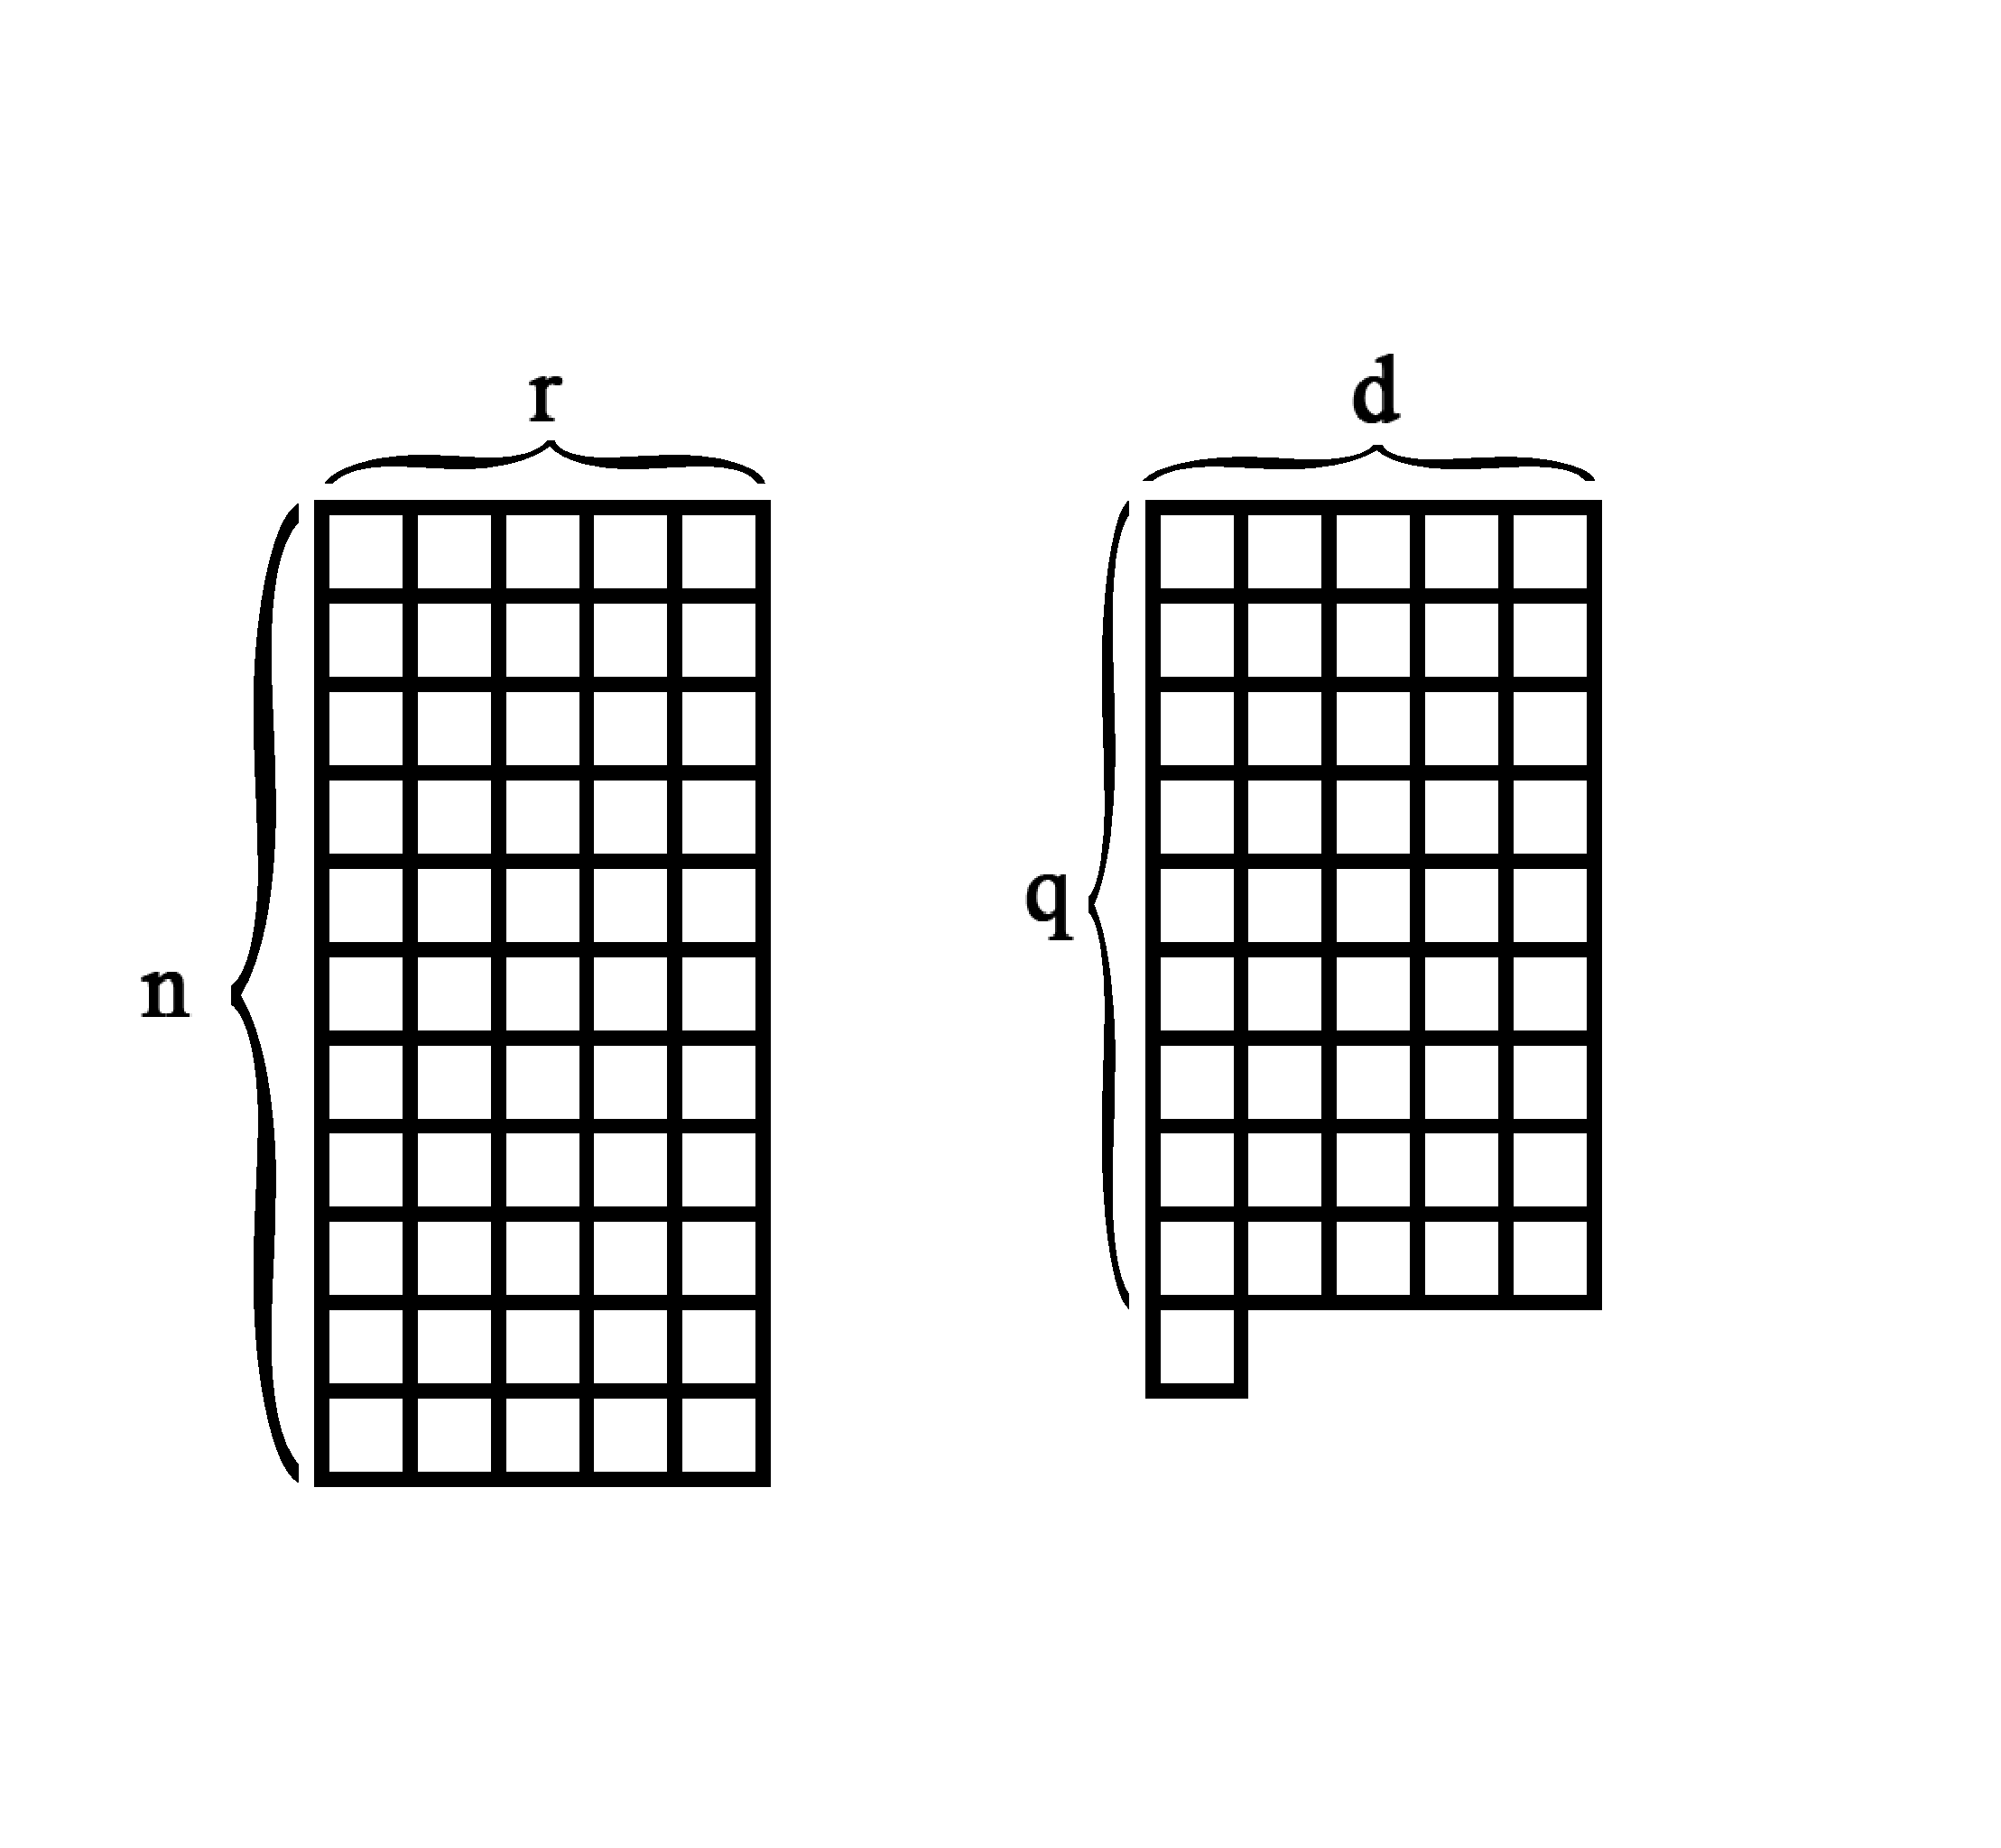
\includegraphics[width=0.4\textwidth]{figs/Young_diagrams.pdf}%
    }{%
        \fbox{\rule{0pt}{2in}\rule{0.7\textwidth}{0pt}}
    }
    \caption{Young diagrams of the representation $S_{\left(q+1, q^{d-1}\right)} V$ and the representation $\left(S_{\left(1^r\right)}V\right)^{\otimes n}$, where $n r=d q+1$.}
    \label{fig:Young_diagrams}
\end{figure}

\begin{smlemma}\label{lem:adjoint_in_end}
    $SU(d)$ representation $\operatorname{End}(V_{\omega_r})$, contains 
    exactly one copy of the adjoint and trivial representations.
\end{smlemma}

\begin{proof}
As in previous proof, we first work in the context of $GL_d(\mathbb{C})$ representations and then restrict ourselves to $SU(d)$ representations.
Since $\Lambda^r V \cong V_{\omega_r}$ as $SU(d)$ representations, it is reasonable to consider $\Lambda^r V \cong S_{\left(1^r\right)}(V)$ as $GL_d(\mathbb{C})$ representation.
First, notice that
$$
    \operatorname{End}(S_{\left(1^r\right)}(V))\cong S_{\left(1^r\right)}(V) \otimes (S_{\left(1^r\right)}(V))^* \cong (\det V)^{-1} \otimes S_{\left(1^r\right)} V \otimes S_{\left(1^{d-r}\right)} V.
$$
Now we apply Pieri's formula in the following form
\[
S_{\left(1^r\right)} V \otimes S_{\left(1^{d-r}\right)} V \cong \bigoplus_{i=0}^{\min (r, d-r)} S_{\left(2^i, 1^{d-2 i}\right)} V
\]
Indeed, starting from $(1^r)$ and multiplying by $(1^{d-r})$ we add a vertical strip of size $d-r$ to the first diagram (according to Pieri's formula). 
Since the first diagram is a single column itself, we have two options: add to an existing row, producing a row of length $2$, or
create a new row, producing a row of length $1$.
The resulting partition is 
$
\left(2^i, 1^{(r-i)+((d-r)-i)}\right)=\left(2^i, 1^{d-2 i}\right) .
$
Multiplicity representation, corresponding to each partition, is one -- again, according to Pieri's formula.
Thus,
\begin{equation}\label{eq:decompositionEnd}
    \operatorname{End}\left(S_{\left(1^r\right)}(V)\right) \cong \bigoplus_{i=0}^{\min (r, d-r)}(\operatorname{det} V)^{-1} \otimes S_{\left(2^i, 1^{d-2 i}\right)} V.
\end{equation}

Now let's find the expression of the adjoint representation as a polynomial $GL_d(\mathbb{C})$-module. On the one side, we have
\[
    \operatorname{End}(V)=V \otimes V^* \cong \mathbf{1} \oplus \mathrm{Ad}
\]
On the other side
\[
    V \otimes V^* \cong(\operatorname{det} V)^{-1} \otimes S_{\left(1\right)} V \otimes S_{\left(1^{d-1}\right)} V
\]
and using Pieri's formula again, we get
\[
    V \otimes V^* \cong (\operatorname{det} V)^{-1} \otimes \left(S_{\left(1^d\right)} V \oplus S_{\left(2,1^{d-2}\right)} V\right)=\mathbf{1} \oplus(\operatorname{det} V)^{-1} \otimes S_{\left(2,1^{d-2}\right)} V
\]
from which we derive
\[
    \mathrm{Ad} \cong(\operatorname{det} V)^{-1} \otimes S_{\left(2,1^{d-2}\right)} V
\]
and from decomposition (\ref{eq:decompositionEnd}) we conclude that
\[
    \operatorname{dim} \operatorname{Hom}_{GL_d(\mathbb{C})}\left(\mathrm{Ad}, \operatorname{End}\left(S_{\left(1^r\right)}(V)\right)\right)=1 .
\]
Finally, let's restrict ourselves to $SU(d)$ representations. To be precise, 
    \[
        S_{\left(1^r\right)}(V)\downarrow_{SU(d)}\cong V_{\omega_r}, \quad \mathrm{Ad}\downarrow_{SU(d)} \cong \mathrm{Ad},
    \]
From \ref{eq:decompositionEnd} we infer that there is exactly one copy of the trivial representation -- term $i=0$.
This completes our proof.
\end{proof}

We define generators of $\mathfrak{su}(d)$ (fundamental representation) in a standard way:
choose $t_a$ that are traceless Hermitian complex $d \times d$ matrices, where:
\begin{equation}\label{eq:sudgenerators}
t_a t_b=\frac{1}{2 d} \delta_{a b} I_d+\frac{1}{2} \sum_{c=1}^{d^2-1}\left(i f_{a b c}+d_{a b c}\right) t_c
\end{equation}
where the $f$ are the structure constants and are antisymmetric in all indices, while the $d$-coefficients are symmetric in all indices.
As a consequence,
$$
\left[t_a, t_b\right]=i \sum_{c=1}^{d^2-1} f_{a b c} t_c, \quad \left\{t_a, t_b\right\}=\frac{1}{d} \delta_{a b} I_d+\sum_{c=1}^{d^2-1} d_{a b c} t_c.
$$
With this definition conventional normalizations are
\begin{equation}\label{eq:sudnormalisation}
\operatorname{Tr}\left(t_a t_b\right)=\frac{1}{2} \delta_{a b}, \quad \sum_{c, e=1}^{d^2-1} d_{a c e} d_{b c e}=\frac{d^2-4}{d} \delta_{a b}.
\end{equation}
We will also use the following identities, which can be easily derived from the definition of generators:
\begin{equation}\label{eq:sudidentities}
    \sum_{m, n=1}^{d^2-1}f_{a m n} f_{b m n}=d \delta_{a b}, \quad \sum_{m, n=1}^{d^2-1}f_{a m n} d_{b m n}=0 , \quad \sum_{m=1}^{d^2-1}d_{a m m}=0 .
\end{equation}

We denote by $\{T_a\}$ the set of operators on $V_{\omega_r}$ that are representation of generators $\{t_a\}$ of $\mathfrak{su}(d)$, omitting the index $r$ for brevity.
Notice that $T_a$ are also traceless Hermitian complex matrices.
We will later need the following normalization 
\begin{equation}\label{eq:sudnormalisation_2}
\operatorname{Tr}_{V_{\omega_r}}\left(T_a T_b\right)=\kappa_{\omega_r} \delta_{a b}, \quad \kappa_{\omega_r}=\frac{1}{2}\binom{d-2}{r-1}.
\end{equation}

\begin{smproposition}\label{prop:SUdcov}
    Let
    $
        \mathcal H_L=V_{\omega_1},\;
        \mathcal H_P=(V_{\omega_r})^{\otimes n}
    $
    and $nr\equiv 1\;(\operatorname{mod} d)$.
    Equip \(\mathcal H_L\) with the fundamental representation of
    \(\mathfrak{su}(d)\), and equip \(\mathcal H_P\) with the transversal
    representation given by
    \begin{equation}
    \begin{gathered}
    t_a \rightarrow T_a \equiv \sum_{i=1}^n T_a^{(i)}, \quad a=\overline{1, d^2-1}
    \end{gathered}
    \end{equation}
    where $T_a^{(i)}$ is a representation of $t_a$ on the $i$-th physical space $V_{\omega_r}$, acting as in Eq.~\eqref{eq:action_on_extirior_power}.
    Then there exist a code space $\mathfrak{su}(d)$-covariant encoding $\mathcal{E}$ with respect to defined physical and logical representations, such that the state seen by the environment after erasure of any single physical qudit is of the form   
    \[
        \rho^{(i)}\left(\rho_L\right)=\frac{I}{\operatorname{dim} V_{\omega_r}}+\frac{1}{n} \frac{1}{2\kappa_{\omega_r}} \sum_a r_a T_a^{(i)} .    
    \]
    Namely, this code space is one of the copies of the fundamental representation $V_{\omega_1}$ in $\left(V_{\omega_r}\right)^{\otimes n}$ which is invariant under cyclic permutations of physical qudits.
\end{smproposition}

\begin{proof}
We recall that from Schur lemma $\left(V_{\omega_r}\right)^{\otimes n}\cong \bigoplus_{\lambda\in \Lambda} V_\lambda\otimes M_{\lambda}$, where $\Lambda$ is a set of irreducible representations of $SU(d)$, 
$V_\lambda$ is the irreducible representation space and $M_\lambda$ is the multiplicity space.

In Lemma~\ref{lem:fundamental_in_extirior_power} we prove that for the choice of individual physical space to be $V_{\omega_r}$ and $n r \equiv 1 (\bmod d)$, it is guaranteed 
that $\operatorname{dim} M_{V_{\omega_1}}>0$.

The linear extension $\Phi^{(i)}:\operatorname{End}(V_{\omega_1})\rightarrow \operatorname{End}(V_{\omega_r})$ of the reduced state map $\rho_L \rightarrow \rho^{(i)}\left(\rho_L\right)$ is an intertwiner of $SU(d)$ representations. 
Logical space as $SU(d)$ representation is
\[
     \text{End}(V_{\omega_1})\cong V_{\omega_1} \otimes (V_{\omega_1})^* \cong \mathbf{1} \oplus \mathrm{Ad}.
\]
For individual system representation $V_{\omega_r}$ we have the following decomposition
\[
    \text{End}(V_{\omega_r})\cong V_{\omega_r} \otimes V_{\omega_r}^* \cong \mathbf{1} \oplus \mathrm{Ad} \oplus \cdots.
\]
From Lemma~\ref{lem:adjoint_in_end} we infer that there is always exactly one copy of the trivial representation and also exactly one copy of the adjoint representation.
As an intertwiner $\Phi^{(i)}$ should have a form
\[
\Phi^{(i)}\cong I_{\mathbf{1}}\otimes A_{M_\mathbf{1}\rightarrow M_\mathbf{1}}\oplus I_{\mathrm{Ad}}\otimes A_{M_\mathrm{Ad}\rightarrow M_\mathrm{Ad}}
\]
and since $\dim M_\mathbf{1}=\dim M_\mathrm{Ad}=1$ we get
\begin{equation}
\begin{gathered}
        \Phi^{(i)}\left(\frac{I_d}{d}\right)=\frac{I_{V_{\omega_r}}}{\operatorname{dim} V_{\omega_r}},\\
        \Phi^{(i)}\left(\sum_a r_a t_a\right)=\beta^{(i)}\sum_a r_a T_a^{(i)}.
\end{gathered}
\end{equation}

Going back to reduced state map $\rho^{(i)}\left(\rho_L\right)$, since logical state has the following form
\[
     \rho_L=\frac{I_d}{d}+\left(\rho_L-\frac{I_d}{d}\right)=\frac{I_d}{d}+\sum_a r_a t_a,
\]
where $\frac{I}{d}$ is in trivial representation and $\rho_L-\frac{I}{d}$ is in adjoint representation, we have that $\rho^{(i)}\left(\rho_L\right)$ has the following form
\[
    \rho^{(i)}\left(\rho_L\right) = \frac{I_{V_{\omega_r}}}{\operatorname{dim} V_{\omega_r}}+\beta^{(i)} \sum_a r_a T_a^{(i)}.
\]
where $\beta^{(i)}$ is some constant that depends on the choice of code space.
Indeed, $\rho^{(i)}\left(\rho_L\right)$ is a covariant map, so it takes a trivial representation to a trivial representation and an adjoint representation.
And since we have chosen $V_{\omega_r}$ such that it contains exactly one copy of the adjoint representation, we have the desired form. Let

\[
    V: V_{\omega_1} \rightarrow V_{\omega_r}^{\otimes n}
\]
our encoding isometry, where $V_{\omega_1}$ is the fundamental representation of $SU(d)$. 
We want to show

\[
V^{\dagger} T_a^{(i)} V=\alpha^{(i)} t_a.
\]
Equivalently, if we define
\begin{equation}\label{eq:Vt_aV}
     K_a^{(i)}:=V^{\dagger} T_a^{(i)} V \in \operatorname{End}\left(V_{\omega_1}\right),
\end{equation}
we need to show
\[
    K_a^{(i)}=\alpha^{(i)} t_a.
\]
From the fact that local generators transform in the adjoint representation, i. e.
\[
     \left(\bigotimes_{k=1}^n U^{(k)}(g)\right) T_a^{(i)} \left(\bigotimes_{k=1}^n U^{(k)}(g)\right)^{\dagger}=\sum_b \operatorname{Ad}_{b a}(g) T_a^{(i)}
\]
and the covariance condition of the encoding map we have
\[
     u(g) K_a^{(i)} u(g)^{\dagger}=\sum_b \operatorname{Ad}_{b a}(g) K_b^{(i)}.
\]
$\operatorname{End}\left(V_{\omega_1}\right)$ contains exactly one copy of adjoint representation
\[
     \operatorname{End}\left(V_{\omega_1}\right) \cong V_{\omega_1} \otimes V_{\omega_1}^* \cong \mathbf{1} \oplus \operatorname{Ad}
\]
which means that by Shur's lemma
\[
     \operatorname{dim} \operatorname{Hom}_{S U(d)}\left(\operatorname{Ad}, \operatorname{End}\left(V_{\omega_1}\right)\right)=1
\]
so we have that $K_a^{(i)}$ is proportional to $t_a$. Now we are to obtain $\beta^{(i)}$ in terms of $\alpha^{(i)}$. We have

\[
     \operatorname{Tr}\left(\rho^{(i)}\left(\rho_L\right) T_a^{(i)}\right)=\beta^{(i)} \sum_b r_b \operatorname{Tr}\left(T_b^{(i)} T_a^{(i)}\right) .
\]
From normalization relations~\eqref{eq:sudnormalisation} and~\eqref{eq:sudnormalisation_2} we get
\[
     \operatorname{Tr}\left(\rho^{(i)}\left(\rho_L\right) T_a^{(i)}\right)=\beta^{(i)} \kappa_{\omega_r} r_a .
\]
and on the other hand, using properties of $\Tr$ and covariance condition of encoding map we get
\[
     \operatorname{Tr}\left(\rho^{(i)}\left(\rho_L\right) T_a^{(i)}\right)=\operatorname{Tr}\left(V \rho_L V^{\dagger} T_a^{(i)}\right)=\operatorname{Tr}\left(\rho_L V^{\dagger} T_a^{(i)} V\right)=\alpha^{(i)} \operatorname{Tr}\left(\rho_L t_a\right) .
\]
from $\rho_L=\frac{I}{d}+\sum_a r_a t_a$, we have
$
     \operatorname{Tr}\left(\rho_L t_a\right)=\frac{1}{2} r_a
$
so on the other hand we have
$
     \operatorname{Tr}\left(\rho^{(i)}\left(\rho_L\right) T_a^{(i)}\right)=\frac{\alpha^{(i)}}{2} r_a .
$
from which we finally obtain the following expression for $\beta^{(i)}$:
\[
     \beta^{(i)}=\frac{1}{2\kappa_{\omega_r}}\alpha^{(i)}  .
\]

Finally, the reduced state on the $i$-th physical qudit has the following form
\[
    \rho^{(i)}\left(\rho_L\right)=\frac{I}{\operatorname{dim} V_{\omega_r}}+\alpha^{(i)} \frac{1}{2\kappa_{\omega_r}} \sum_a r_a T_a^{(i)} .
\]
Using the same code construction for symmetric code as we did for $SU(2)$ case (see the proof of the Proposition~\ref{prop:SU2cov}), namely, making code space invariant under cyclic shifts, our code space is such that $\alpha^{(i)}=\frac{1}{n}$ for all $i$, which gives the desired form of reduced state.

\end{proof}


\begin{smproposition}\label{prop:SUdcovfidelity}
    For the encoding $\mathcal{E}$ defined in the Proposition~\ref{prop:SUdcov} and noise channel $\mathcal{N}(\sigma)=\sum_{i=1}^n p_i \ket{i}\bra{i}_F \otimes \ket{e}\bra{e}_{A_i} \otimes \operatorname{Tr}_i(\sigma)$ the worst-case entanglement fidelity is
    \[
        F(\widehat{\mathcal{N} \circ \mathcal{E}}, \Lambda_0)=1-\frac{(d-1)^2(d+1)}{8 r(d-r)}\frac{1}{n^2}+O\left(n^{-3}\right),
    \]
    where we take $\Lambda_0(\rho)=\operatorname{Tr}(\rho)\omega_{\text{flag}}\otimes\frac{I_{V_{\omega_r}}}{\operatorname{dim} V_{\omega_r}}$, where $\omega_{\text {flag}}=\sum p_i|i\rangle\langle i|_{F_E}$.
\end{smproposition}

\begin{proof}
In this section, we will calculate the worst-case fidelity of $SU(d)$-covariant codes with flagged erasure error model
in the same way as we did for $SU(2)$-covariant codes. 
For the later calculations we will use notation $\beta:=\frac{1}{n} \frac{1}{2\kappa_{\omega_r}}$, $D=\operatorname{dim} V_{\omega_r}$.
Since reduced states are identical on each site, the complementary channel becomes
\[
        \widehat{\mathcal{N} \circ \mathcal{E}}(\rho)=\omega_{\text {flag }} \otimes \left(\frac{I_D}{D}+ \beta \sum_a r_a T_a^{(1)}\right),
\]
where $\omega_{\text {flag }}=\sum p_i|i\rangle\langle i|_{F_E}$ is the flag state. We chose the fixed channel to be 
$$
\Lambda_0(\rho)=\operatorname{Tr}(\rho)\cdot \omega_{\text {flag }}\otimes \frac{I_{D}}{D} \equiv \operatorname{Tr}(\rho)\cdot \omega_{\text {flag }}\otimes \tau.
$$ 
We drop flag state $\omega_{\text {flag }}$, since fidelity is invariant under 
tensor multiplication on the same state; we also omit the index of a site $(1)$.

As we know from \ref{fidelity_opt} the optimum of $F_{\rho}(\widehat{\mathcal{N} \circ \mathcal{E}}, \Lambda_0)$ is attained on the chaotic state $\frac{I_d}{d}$, its purification is maximally entangled state $\ket{\Psi}=\frac{1}{\sqrt{d}}\sum |r\rangle \otimes|r\rangle $. We have to compute $(\widehat{\mathcal{N} \circ \mathcal{E}} \otimes \mathrm{id})(\ket{\Psi}\bra{\Psi})$ and $(\Lambda_0 \otimes \mathrm{id})(\ket{\Psi}\bra{\Psi})$.
We define the linear extension of the reduced state channel to all complex matrices as follows
$$
\Phi: \operatorname{End}\left(V_{\omega_1}\right) \rightarrow \operatorname{End}\left(V_{\omega_r}\right), \quad \Phi\left(t_a\right):=T_a, \quad \Phi\left(\frac{I_d}{d}\right):=\tau
$$
and we will use the following notation for our derivations
\begin{equation}\label{eq:matr_units}
     E_{r s}:=|r\rangle\langle s|, \quad F_{r s}:=E_{r s}-\delta_{r s} \frac{I_d}{d}.
\end{equation}
For the constant channel, we have
\[
     \eta_{1/d}:=(\Lambda_0 \otimes \mathrm{Id})\left(\ket{\Psi}\bra{\Psi}\right)=\tau \otimes \frac{I_d}{d}.
\]  
For the complementary channel using 
$
\widehat{\mathcal{N} \circ \mathcal{E}}\left(E_{r s}\right)=\delta_{r s} \tau+\beta \Phi\left(F_{r s}\right) .
$
we define 
\[
\begin{gathered}
     \sigma_{1/d}:=\left(\widehat{\mathcal{N} \circ \mathcal{E}} \otimes \mathrm{Id}\right)\left(\ket{\Psi}\bra{\Psi}\right)=\frac{1}{d}\sum_{r, s=1}^d \widehat{\mathcal{N} \circ \mathcal{E}}\left(E_{r s}\right) \otimes|r\rangle\langle s| =\\
     =\frac{1}{d}\sum_{r, s=1}^d \left(\delta_{r s} \tau+\beta \Phi\left(F_{r s}\right)\right) \otimes|r\rangle\langle s| .
\end{gathered}
\]
We obtain the following expression for fidelity
\[
     f\left(\sigma_{1/d}, \eta_{1/d}\right)=\operatorname{Tr}\sqrt{\sqrt{\eta_{1/d}} \sigma_{1/d} \sqrt{\eta_{1/d}}}=\operatorname{Tr} \sqrt{\frac{1}{Dd^2}\left[\delta_{r s} \tau+\beta \Phi\left(F_{r s}\right)\right]_{r, s=1}^d}.
\]
Now, we recall that $\Phi$ actually acts as follows
\[
        \Phi\left(F_{a b}\right)=T_{a b}^{(r)}-\delta_{a b} \frac{r}{d} I_D,
\]
where $T_{a b}^{(r)}$ is the representation of $F_{a b}$ in the adjoint representation of $SU(d)$ and defined as follows
\[
    T_{a b}^{(r)}\left(v_1 \wedge \cdots \wedge v_r\right)=\sum_{m=1}^r v_1 \wedge \cdots \wedge E_{a b} v_m \wedge \cdots \wedge v_r
\]
so we can rewrite the expression for fidelity as follows
\[
\begin{aligned}
    f\left(\sigma_{1/d}, \eta_{1/d}\right)&=\operatorname{Tr} \sqrt{\frac{1}{Dd^2}\left[\delta_{a b} \tau+\beta \left(T_{a b}^{(r)}-\delta_{a b} \frac{r}{d} I_D\right)\right]_{a, b=1}^d}\\&\equiv\frac{1}{d \sqrt{D}} \operatorname{Tr} \sqrt{\frac{I_{D d}}{D}+\beta B} .
\end{aligned}
\]
where 
\[
    B=\left(\begin{array}{cccc}
    T_{11}^{(r)}-\frac{r}{d} I_D & T_{12}^{(r)} & \cdots & T_{1 d}^{(r)} \\
    T_{21}^{(r)} & T_{22}^{(r)}-\frac{r}{d} I_D & \cdots & T_{2 d}^{(r)} \\
    \vdots & \vdots & \ddots & \vdots \\
    T_{d 1}^{(r)} & T_{d 2}^{(r)} & \cdots & T_{d d}^{(r)}-\frac{r}{d} I_D
    \end{array}\right).
\]
We are now to expand this expression up to a leading order in $\beta$
\[
\begin{aligned}
        f\left(\sigma_{1/d}, \eta_{1/d}\right)&=1+\frac{\beta}{2 d} \operatorname{Tr} B-\frac{D \beta^2}{8 d} \operatorname{Tr} B^2+O\left(\beta^3\right)\\&=1-\frac{D^2 \beta^2}{8 d}\left(r(d-r+1)-\frac{r^2}{d}\right)+O\left(\beta^3\right)
\end{aligned}
\]
where we use the fact that $\operatorname{Tr} B=0$ and $\operatorname{Tr} B^2=D\left(r(d-r+1)-\frac{r^2}{d}\right)$. Indeed, 
$$
\begin{aligned}
    \operatorname{Tr} B^2&=\sum_{a, b=1}^d \operatorname{Tr}_{V_{\omega_r}}\left(\Phi\left(F_{a b}\right) \Phi\left(F_{b a}\right)\right)=\sum_{a\neq b}^d\operatorname{Tr}\left(T_{a b}^{(r)} T_{b a}^{(r)}\right)+\sum_{a=1}^d \operatorname{Tr}\left(T_{a a}^{(r)}-\frac{r}{d} I_D\right)^2\\&=d(d-1)\binom{d-2}{r-1}+d\frac{Dr(d-r)}{d^2}=D\left(r(d-r+1)-\frac{r^2}{d}\right)
\end{aligned}
$$
Finally, if we substitute $\beta=\frac{1}{n} \frac{1}{2\kappa_{\omega_r}}$, $D=\operatorname{dim} V_{\omega_r}$ and $\kappa_{\omega_r}=\frac{1}{2}\binom{d-2}{r-1}$ into $F(\widehat{\mathcal{N} \circ \mathcal{E}}, \Lambda_0)=f(\sigma_{1/d}, \eta_{1/d
})$ we get a desired expression for fidelity.
\end{proof}

\subsection{Explicit Decoder construction}\label{subsec:supple_decoder}

In this section, we will construct an explicit decoder for $SU(d)$-covariant codes with the erasure error model.
For this, we will use the Petz recovery map, which is defined as follows
\begin{smdefinition}
    For a given channel $\mathcal{N}$ and reference state $\omega$, the Petz map $\mathcal{P}_{\omega, \mathcal{N}}$ is defined as:
    \[
        \mathcal{P}_{\omega, \mathcal{N}}(\sigma)=\omega^{1 / 2} \mathcal{N}^*\left(\mathcal{N}(\omega)^{-1 / 2} \sigma \mathcal{N}(\omega)^{-1 / 2}\right) \omega^{1 / 2},
    \]
    where $\mathcal{N}^*$ is the adjoint of $\mathcal{N}$ with respect to the Hilbert-Schmidt inner product, and $\omega$ is so-called reference state.
\end{smdefinition}

\begin{smtheorem}\label{thm:petz_decoder_explicit}
For the encoding $\mathcal E$ and the flagged single-qudit erasure channel $\mathcal N$ defined in Theorem~\ref{thrm:sudscale}, the Petz recovery map with reference state $\omega=I_d/d$ has the form
$$
\mathcal R_{\mathrm{Petz}}(X)
=
\sum_{i:,p_i>0}
V^\dagger
\left(
S_i^{-1/2}
\langle i,e|X|i,e\rangle_{F,A_i}
S_i^{-1/2}
\otimes I_{A_i}
\right)
V,
$$
where $V$ is the encoding isometry and
$$
S_i
:=
\operatorname{Tr}_i\left(VV^\dagger\right).
$$
Moreover, this recovery is near-optimal in the sense that
$$
    d\left(
    \mathcal R_{\mathrm{Petz}}
    \circ
    \mathcal N
    \circ
    \mathcal E,
    \mathrm{id}
    \right)
    =
    O(n^{-1}) .
$$
\end{smtheorem}

\begin{proof}
Define the erased channel for site $i$ by
$
    \mathcal{C}_i\left(\rho_L\right):=\operatorname{Tr}_{i}\left(V \rho_L V^{\dagger}\right).
$
Our noise channel in this notation can be written as
$
    \mathcal{N}(\sigma)=\sum_{i=1}^n p_i\ket{i}\bra{i}_F \otimes \ket{e}\bra{e}_{A_i}\otimes \mathcal{C}_i.
$
We take a reference state $\omega$ to be the chaotic state $\frac{I}{d}$, which is the only $SU(d)$-invariant state on logical space. We get
\[
    \mathcal{C}_i\left(\omega\right)=\frac{1}{d} \operatorname{Tr}_i\left(V V^{\dagger}\right)=\frac{S_i}{d},
\]
where we defined $S_i:=\operatorname{Tr}_i\left(V V^{\dagger}\right)$. One can easily check that
\[
    \mathcal{C}_i^{\dagger}(Y)=V^{\dagger}\left(Y \otimes I_{W_i}\right) V
\]
where we denoted $W_i$ as the Hilbert space associated with site $i$. Thus, the recovery map is given by
\[
    \mathcal{R}_{\mathrm{Petz}}(X)=\sum_{i: p_i>0} V^{\dagger}\left(S_i^{-1 / 2} \langle i, e| X|i,e\rangle_{F, A_i} S_i^{-1 / 2} \otimes I_{W_i}\right) V,
\]
where the inverse should always be understood as the inverse on the support of $S_i$. Now, let's explore the performance of this decoder, i. e. find $F\left(\mathcal{R}_{\mathrm{Petz}} \circ \mathcal{N}\circ \mathcal{E}, \mathrm{id}\right)$, since we 
are in AQECC setting. We denote
\[
    \Phi:=\mathcal{R}_{\mathrm{Petz}} \circ \mathcal{N}\circ \mathcal{E}
\]
and let's analyze the structure of $\Phi$. First of all, $\Phi: \operatorname{End}(\mathcal{H}_L)\rightarrow \operatorname{End}(\mathcal{H}_L)$ is a 
$SU(d)$-covariant map, i. e.
\[
    \Phi\left(u(g) \rho u(g)^{\dagger}\right)=u(g) \Phi(\rho) u(g)^{\dagger}, \quad \forall g \in SU(d).
\]
Indeed, $\mathcal{C}_i\left(u(g) \rho u(g)^{\dagger}\right)=U^{\bar{i}}(g) \mathcal{C}_i(\rho) \left(U^{\bar{i}}(g)\right)^{\dagger}$ and $S_i^{-1 / 2}$ commutes with $U^{\bar{i}}(g)$ on the support of $S_i$. So it has to take the following form
\[
    \Phi(\rho)=\lambda_{\mathrm{Petz}} \rho+\left(1-\lambda_{\mathrm{Petz}}\right) \frac{I_d}{d} \operatorname{Tr} \rho,
\]
that is basically a depolarizing channel with depolarizing parameter $\lambda_{\mathrm{Petz}}$. Let's show that this depolarizing parameter is given by
\begin{equation}\label{eq:lambdaPetz}
    \lambda_{\text{Petz}}=\frac{2}{d^2-1}\sum_{i=1}^n p_i \sum_{a=1}^{d^2-1} \operatorname{Tr}\left[S_i^{-1 / 2} \mathcal{C}_i\left(t_a\right) S_i^{-1 / 2} \mathcal{C}_i\left(t_a\right)\right] .
\end{equation}
Indeed, since $\Phi\left(t_a\right)=\lambda_{\text{Petz}} t_a$, we have
$$
\operatorname{Tr}\left(t_a \Phi\left(t_a\right)\right)=\frac{1}{2} \lambda_{\text{Petz}},
$$
where we used $\operatorname{Tr}\left(t_a t_b\right)=\frac{1}{2} \delta^{a b}$. Summing over $a$,
$$
\lambda_{\text{Petz}}=\frac{2}{\left(d^2-1\right)} \sum_{a=1}^{d^2-1} \operatorname{Tr}\left(t_a \Phi\left(t_a\right)\right)
$$
Now substitute the Petz formula:
$$
\Phi_{\mathrm{Petz}}\left(t_a\right)=\sum_i p_i V^{\dagger}\left(S_i^{-1 / 2} \mathcal{C}_i\left(t_a\right) S_i^{-1 / 2} \otimes I_{A_i}\right) V.
$$
Hence
$$
\operatorname{Tr}\left(t_a \Phi_{\text{Petz}}\left(t_a\right)\right)=\sum_i p_i \operatorname{Tr}\left[S_i^{-1 / 2} \mathcal{C}_i\left(t_a\right) S_i^{-1 / 2} \mathcal{C}_i\left(t_a\right)\right]
$$
where we used the partial-trace identity
$
\operatorname{Tr}\left(X\left(Y \otimes I_W\right)\right)=\operatorname{Tr}\left(\operatorname{Tr}_W(X) Y\right),
$
with $X=V t^a V^{\dagger}$ and $Y=A^{-1 / 2} \mathcal{C}_i\left(t^a\right) A^{-1 / 2}$, gives desired expression for $\lambda_{\mathrm{Petz}}$.

For a pure state \(\psi=|\psi\rangle\langle\psi|\), we have \(\Phi_{\mathrm{Petz}}(\psi)=\lambda_{\mathrm{Petz}}\psi+(1-\lambda_{\mathrm{Petz}})I_d/d\). Since the target state is pure, the root fidelity is
\[
f(\Phi_{\mathrm{Petz}}(\psi),\psi)
=
\sqrt{\langle\psi|\Phi_{\mathrm{Petz}}(\psi)|\psi\rangle}
=
\sqrt{\lambda_{\mathrm{Petz}}+\frac{1-\lambda_{\mathrm{Petz}}}{d}} .
\]
This expression is independent of \(\psi\). Hence
\[
\eta_{\mathrm{Petz}}^{\mathrm{st}}
:=
1-\min_{\psi}f^2(\Phi_{\mathrm{Petz}}(\psi),\psi)
=
\frac{d-1}{d}(1-\lambda_{\mathrm{Petz}}).
\]

Our channel fidelity is defined as the minimum over \(\rho\) of \(F_\rho(\Phi_{\mathrm{Petz}},\mathrm{id})=f((\Phi_{\mathrm{Petz}}\otimes\mathrm{id})(|\psi_\rho\rangle\langle\psi_\rho|),|\psi_\rho\rangle\langle\psi_\rho|)\), where \(|\psi_\rho\rangle\) purifies \(\rho\). For the depolarizing channel \(\Phi_{\mathrm{Petz}}\), one finds
\[
(\Phi_{\mathrm{Petz}}\otimes \mathrm{id})(|\psi_\rho\rangle\langle\psi_\rho|)
=
\lambda_{\mathrm{Petz}}|\psi_\rho\rangle\langle\psi_\rho|
+(1-\lambda_{\mathrm{Petz}})\frac{I_d}{d}\otimes \rho_R .
\]
Since the target is pure, this gives \(F_\rho(\Phi_{\mathrm{Petz}},\mathrm{id})=\sqrt{\lambda_{\mathrm{Petz}}+\frac{1-\lambda_{\mathrm{Petz}}}{d}\operatorname{Tr}(\rho^2)}\). This quantity is minimized at \(\rho=I_d/d\), i.e. when \(\operatorname{Tr}(\rho^2)=1/d\). Therefore
\[
F(\Phi_{\mathrm{Petz}},\mathrm{id})
=
\sqrt{\lambda_{\mathrm{Petz}}+\frac{1-\lambda_{\mathrm{Petz}}}{d^2}} .
\]
Equivalently,
\[
\eta_{\mathrm{Petz}}^{\mathrm{ent}}
:=
1-F^2(\Phi_{\mathrm{Petz}},\mathrm{id})
=
\frac{d^2-1}{d^2}(1-\lambda_{\mathrm{Petz}})
=
\frac{d+1}{d}\eta_{\mathrm{Petz}}^{\mathrm{st}} .
\]

Thus, the exact worst-case channel fidelity of the Petz-recovered channel is determined by \(\lambda_{\mathrm{Petz}}\). However, analyzing this expression directly would require obtaining the scaling of \(\lambda_{\mathrm{Petz}}\) in terms of \(n\). This, in turn, requires a careful analysis of Eq.~\eqref{eq:lambdaPetz}, namely of the scaling of \(A\) and \(\mathcal C_i(\bar t_a)\) with \(n\). This is highly nontrivial, because these operators lie in the adjoint representation inside \((V_{\omega_r})^{\otimes(n-1)}\), where the adjoint component appears with large multiplicity, in contrast to the single-qudit case. Similar complications will appear below in the analysis of multi-qudit erasure errors.

We leave a direct analysis of \(\lambda_{\mathrm{Petz}}\) for future work. Instead, we use the near-optimality theorem of Ng and Mandayam for the transpose channel, equivalently the Petz recovery map with the maximally mixed code state as reference state~\cite{Ng2010}. Their result states that
\[
\eta_{\mathrm{Petz}}^{\mathrm{st}}
\le
\eta_{\mathrm{op}}^{\mathrm{st}}
\frac{(d+1)-\eta_{\mathrm{op}}^{\mathrm{st}}}
{1+(d-1)\eta_{\mathrm{op}}^{\mathrm{st}}},
\]
where \(\eta_{\mathrm{op}}^{\mathrm{st}}:=\min_{\mathcal R}[1-\min_{\psi}f^2(\psi,(\mathcal R\circ\mathcal C)(\psi))]\). Moreover, the optimal state-fidelity error is bounded by the optimal entanglement-fidelity error, \(\eta_{\mathrm{op}}^{\mathrm{st}}\leq \eta_{\mathrm{op}}^{\mathrm{ent}}\). Therefore, since Theorem~$2$ from the main part of the paper gives \(\eta_{\mathrm{op}}^{\mathrm{ent}}=O(n^{-2})\), we obtain \(\eta_{\mathrm{Petz}}^{\mathrm{st}}=O(n^{-2})\). Finally, using \(\eta_{\mathrm{Petz}}^{\mathrm{ent}}=\frac{d+1}{d}\eta_{\mathrm{Petz}}^{\mathrm{st}}\), we conclude that
\[
\eta_{\mathrm{Petz}}^{\mathrm{ent}}=O(n^{-2}).
\]
This gives the desired scaling.

\end{proof}

\subsection{Performance under arbitrary single-qudit errors}\label{subsec:supple_arb_noise}

\begin{smlemma}\label{lem:dual_to_arb}
    Let $\mathcal{E}$ be the encoding map defined by $\mathcal{E}(\rho_L):=V\rho_L V^{\dagger}$ and
    $
        \mathcal N(\sigma)
        =
        \sum_{S\in\mathcal S}
        p_S
        |S\rangle\langle S|_F
        \otimes
        \left(\mathcal N_S\otimes \mathrm{id}_{\bar S}\right)(\sigma)
    $
    be a noise model, where $\mathcal{N}_S$ is an arbitrary noise channel acting on the subsystem $S$. Then a complementary channel to $\mathcal{N}\circ \mathcal{E}$ is given as follows:
    \[
        \widehat{\mathcal{N} \circ \mathcal{E}}\left(\rho_L\right)
        =
        \sum_{S\in\mathcal S}
        p_S
        |S\rangle\langle S|_{F_E}
        \otimes
        \widehat{\mathcal{N}_S}\left(\rho^{(S)}\left(\rho_L\right)\right).
    \]
\end{smlemma}

\begin{proof}
    Consider a Stinespring dilation of the noise channel $\mathcal{N}$ of the form
    \[
        \mathcal{W}
        =
        \sum_{S\in\mathcal S}
        \sqrt{p_S}
        |S\rangle_F
        \otimes
        |S\rangle_{F_E}
        \otimes
        \left(W_S \otimes I_{\bar S}\right),
    \]
    where $W_S$ is a Stinespring dilation of $\mathcal{N}_S$. Notice that
\[
    \begin{aligned}
    \widehat{\mathcal{N}\circ\mathcal{E}}(\rho_L)
    &=
    \operatorname{Tr}_{\mathrm{rec}}
    \left[
    \mathcal W V\rho_LV^\dagger \mathcal W^\dagger
    \right]
    \\
    &=
    \sum_{S,T\in\mathcal S}
    \sqrt{p_Sp_T}\,
    \operatorname{Tr}_F(|S\rangle\langle T|_F)\,
    |S\rangle\langle T|_{F_E}
    \otimes
    \operatorname{Tr}_{B_S\bar S}
    \left[
    (W_S\otimes I_{\bar S})
    V\rho_LV^\dagger
    (W_T^\dagger\otimes I_{\bar T})
    \right]
    \\
    &=
    \sum_{S\in\mathcal S}
    p_S |S\rangle\langle S|_{F_E}
    \otimes
    \operatorname{Tr}_{B_S\bar S}
    \left[
    (W_S\otimes I_{\bar S})
    V\rho_LV^\dagger
    (W_S^\dagger\otimes I_{\bar S})
    \right]
    \\
    &=
    \sum_{S\in\mathcal S}
    p_S |S\rangle\langle S|_{F_E}
    \otimes
    \operatorname{Tr}_{B_S}
    \left[
    W_S
    \operatorname{Tr}_{\bar S}(V\rho_LV^\dagger)
    W_S^\dagger
    \right]
    \\
    &=
    \sum_{S\in\mathcal S}
    p_S |S\rangle\langle S|_{F_E}
    \otimes
    \widehat{\mathcal N_S}\bigl(\rho^{(S)}(\rho_L)\bigr),
    \end{aligned}
\]
where $B_S$ is the output Hilbert space of the local noise channel acting on the subsystem $S$.
\end{proof}
\begin{smtheorem}\label{thrm:sudscale_general}
            Let
$
    \mathcal H_L=V_{\omega_1},\;
    \mathcal H_P=(V_{\omega_r})^{\otimes n}
$
and $nr\equiv 1\;(\operatorname{mod} d)$.
Equip \(\mathcal H_L\) with the fundamental representation of
\(\mathfrak{su}(d)\), and equip \(\mathcal H_P\) with the transversal
representation given by
\begin{equation}\label{eq:global_generators}
\begin{gathered}
t_a \rightarrow T_a \equiv \sum_{i=1}^n T_a^{(i)}, \quad a=\overline{1, d^2-1},
\end{gathered}
\end{equation} 
where $T_a^{(i)}$ is a representation of $t_a$ on the $i$-th physical space $V_{\omega_r}$, acting as in Eq.~\eqref{eq:action_on_extirior_power}. If encoding $\mathcal{E}$, which is $\mathfrak{su}(d)$-covariant with respect to defined physical and logical representations,  defines a code space invariant under cyclic permutations of physical qudits, then $\mathcal{E}$ is $\Theta\left(\frac{1}{\sqrt{n}}\right)$-approximate against arbitrary single-qudit noise channel $\mathcal{N}(\sigma)=\sum_{i=1}^n p_i|i\rangle\left\langle\left. i\right|_F \otimes\left(\mathcal{N}_i \otimes \mathrm{id}_{\bar{i}}\right)(\sigma),\right.$.
\end{smtheorem}
\begin{proof}
In Proposition~\ref{prop:SUdcov} we obtained the following form of the reduced state on the \(i\)-th physical qudit:
\[
\rho^{(i)}(\rho_L)
=
\frac{I_{V_{\omega_r}}}{\dim V_{\omega_r}}
+
\frac{1}{n}\mathcal A_i\left(\rho_L-\frac{I_d}{d}\right),
\]
where the linear map \(\mathcal A_i\) is defined on the traceless part by
\[
\mathcal A_i\left(\sum_a r_a t_a\right)
=
\frac{1}{2\kappa_{\omega_r}}\sum_a r_a T_a^{(i)} .
\]
Therefore, using Lemma~\ref{lem:dual_to_arb}, we can rewrite the complementary channel as
\[
\widehat{\mathcal{N} \circ \mathcal{E}}(\rho_L)
=
\sum_i p_i |i\rangle\langle i|_{F_E}\otimes
\left[
\widehat{\mathcal N}_i\left(\frac{I_{V_{\omega_r}}}{\dim V_{\omega_r}}\right)
+
\frac{1}{n}
\widehat{\mathcal N}_i\mathcal A_i\left(\rho_L-\frac{I_d}{d}\right)
\right].
\]
It is then natural to take
\[
\Lambda_0(\rho_L)
=
\operatorname{Tr}(\rho_L)
\sum_i p_i |i\rangle\langle i|_{F_E}\otimes
\widehat{\mathcal N}_i\left(\frac{I_{V_{\omega_r}}}{\dim V_{\omega_r}}\right),
\]
which is a constant channel, i. e. it is independent of \(\rho_L\). We now estimate \(F(\widehat{\mathcal{N} \circ \mathcal{E}},\Lambda_0)\).

We compute \(F_\rho(\widehat{\mathcal{N} \circ \mathcal{E}},\Lambda_0)=f(\sigma_\rho,\eta_\rho)\), where
\[
\sigma_\rho
:=
(\widehat{\mathcal{N}\circ\mathcal{E}}\otimes \mathrm{id})
(|\psi_\rho\rangle\langle\psi_\rho|),
\qquad
\eta_\rho
:=
(\Lambda_0\otimes \mathrm{id})
(|\psi_\rho\rangle\langle\psi_\rho|)
\]
and \(|\psi_\rho\rangle\) is a purification of \(\rho\). By the Fuchs--van de Graaf inequality, we have
\[
\begin{aligned}
1-f(\sigma_\rho,\eta_\rho)
&\leq
\frac{1}{2}\left\|\sigma_\rho-\eta_\rho\right\|_1 \\
&=
\frac{1}{2n}
\sum_i p_i
\left\|
\left((\widehat{\mathcal N}_i\circ \mathcal A_i)\otimes \mathrm{id}_R\right)
\left[
|\psi_\rho\rangle\langle\psi_\rho|
-
\frac{I_d}{d}\otimes \rho_R
\right]
\right\|_1 \\
&\leq
\frac{1}{2n}
\sum_i p_i
\left\|
(\mathcal A_i\otimes \mathrm{id}_R)
\left[
|\psi_\rho\rangle\langle\psi_\rho|
-
\frac{I_d}{d}\otimes \rho_R
\right]
\right\|_1 \\
&\leq
\frac{C_{\omega_r}}{2n}
\left\|
|\psi_\rho\rangle\langle\psi_\rho|
-
\frac{I_d}{d}\otimes \rho_R
\right\|_1 \\
&\leq
\frac{C_{\omega_r}}{n}.
\end{aligned}
\]
Here, in the third line, we used contractivity of the trace norm under the CPTP map \(\widehat{\mathcal N}_i\), and \(C_{\omega_r}:=\max_i|\mathcal A_i\otimes \mathrm{id}_R|_{1\to 1}\). This constant depends only on the fixed physical representation \(V_{\omega_r}\), and not on \(n\).

Therefore,
\[
F_\rho(\widehat{\mathcal{N} \circ \mathcal{E}},\Lambda_0)
\geq
1-\frac{C_{\omega_r}}{n}
\qquad
\forall \rho ,
\]
and hence
\[
F(\widehat{\mathcal{N} \circ \mathcal{E}},\Lambda_0)
=
\min_\rho F_\rho(\widehat{\mathcal{N} \circ \mathcal{E}},\Lambda_0)
\geq
1-\frac{C_{\omega_r}}{n}.
\]
By the same arguments as in the \(SU(2)\) case and from Proposition~\ref{prop:SUdcovfidelity}, there exists a recovery map \(\mathcal R\) such that
\[
d(\mathcal R\mathcal N\mathcal E,\mathrm{id})
\leq
\sqrt{\frac{2C_{\omega_r}}{n}}.
\]
Thus our encoding \(\mathcal E\) is \(\varepsilon\)-approximate with \(\varepsilon=O(n^{-1/2})\).

\end{proof}

\subsection{Performance under multi-qudit erasure errors}\label{subsec:supple_multi_erasure_noise}

The following Lemmas~\ref{lem:M_module_irreducibility}-\ref{lem:3-body_action} are axiliary results that we will need for our analysis of multi-qudit erasure errors and thus can be skipped on first reading.
For notation see Section~\ref{sec:supple_sud} and Nomenclature section.

\begin{smlemma}\label{lem:M_module_irreducibility}
    Let $M_{\omega_1}$ be a multiplicity space of the fundamental $SU(d)$ representation $V_{\omega_1}$ in $\left(V_{\omega_1}\right)^{\otimes n}$, where $n\equiv 1 \pmod{d}$. 
    Then $M_{\omega_1}$ is an irreducible $S_n$-module, namely the Specht module $[q+1, q^{d-1}]$, where $q=\frac{n-1}{d}$.
\end{smlemma}

\begin{proof}
    We recall the notation $V=\C^d$. As always, we first work in the context of $GL_d(\mathbb{C})$ representations and then restrict ourselves to $SU(d)$ representations. 
    From the Schur-Weil duality, we have the following decomposition
    \[
        V^{\otimes n} \cong \bigoplus_{\lambda \vdash n, \ell(\lambda) \leq d} S_\lambda(V) \otimes[\lambda],
    \]
    where $S_\lambda(V)$ is $GL_d(\mathbb{C})$-module and $[\lambda]$ is irreducible $S_n$-module, known as Specht module.
    If we restrict this decomposition to $SU(d)$, then we get
    \[
        V^{\otimes n}\downarrow_{SU(d)}\cong V_{\omega_1}^{\otimes n} \cong \bigoplus_{\lambda \vdash n, \ell(\lambda) \leq d}\left(S_\lambda(V) \downarrow_{S U(d)}\right) \otimes[\lambda],
    \]
    where $S_\lambda(V) \downarrow_{S U(d)}$ is the restriction of $GL_d(\mathbb{C})$-module $S_\lambda(V)$ to $SU(d)$. 
    The decomposition is basically the same as for $GL_d(\mathbb{C})$ case, but the main difference
    is that $S_\lambda(V) \downarrow_{S U(d)}$ may coincide with $S_\mu(V) \downarrow_{S U(d)}$ for $\lambda \neq \mu$, 
    so multiplicity of $V_{\omega_1}$ as a representation of $SU(d)$ requires a careful analysis.
    Multiplicity space $M_{\omega_1}$ is described by the following formula
    \[
        M_{\omega_1}\cong \operatorname{Hom}_{S U(d)}\left(V_{\omega_1}, V_{\omega_1}^{\otimes n}\right) \cong \bigoplus_{\lambda \vdash n, \ell(\lambda) \leq d} \operatorname{Hom}_{S U(d)}\left(V_{\omega_1}, S_\lambda(V) \downarrow_{S U(d)}\right) \otimes[\lambda],
    \]
    so we can write the following
    \[
        M_{\omega_1} \cong \bigoplus_{\lambda \vdash n, \ell(\lambda) \leq d} m_\lambda[\lambda],
    \]
    where since $S_\lambda(V)$ is still irreducible as a representation of $SU(d)$, we have $m_{\lambda}\in \{0,1\}$ for every
    $\lambda$.
    We need to show that $m_\lambda=1$ for exactly one $\lambda$. Indeed,
    $S_\lambda(V) \downarrow_{S U(d)} \cong V_{\omega_1}$ happens exactly iff $\lambda=\left(q+1, q^{d-1}\right)$ for some $q\geq 0$.
    Since also $|\lambda|=n$, we have $n=(q+1)+q(d-1)=d q+1$, so $q=\frac{n-1}{d}$ is an integer. 
    Therefore,
    \[
        M_{\omega_1} \cong\left[q+1, q^{d-1}\right],
    \]
    which proves the lemma.
\end{proof}

\begin{smlemma}\label{lem:dimension_formula}
    Let $[q+1, q^{d-1}]$ be the Specht module corresponding to the partition $(q+1, q^{d-1})$. Then
    \[
        \operatorname{dim} [q+1, q^{d-1}] = \frac{(d q+1)!d!\prod_{i=0}^{d-2} i!}{(q+d)!\prod_{i=0}^{d-2}(q+i)!}.
    \]
\end{smlemma}

\begin{proof}
    The general formula for the dimension of Specht module $[\lambda]$ corresponding to the partition $\lambda$ is given by the hook-length formula, i. e.
    \[
        \operatorname{dim} [\lambda] = \frac{n!}{\prod_{(i, j) \in \lambda} h_{i j}} .
    \]
    where $h_{ij}$ is the hook length of the box in the $i$-th row and $j$-th column, precisely
    \[
        h_{i j}=\#\{\text { boxes to the right of }(i, j)\}+\#\{\text { boxes below }(i, j)\}+1 .
    \]
    It can also be expressed as
    $
        h_{i j}=\lambda_i-j+\lambda_j^{\prime}-i+1 .
    $
    Our Young diagram has the shape of a rectangle with an extra box in the top right corner, and its transpose 
    has the shape of a rectangle with an extra box in the bottom left corner, i. e.
    $$
        \lambda=(q+1, \underbrace{q, \ldots, q}_{d-1 \text { times }}), \quad \lambda'=(\underbrace{d, d, \ldots, d}_{q \text { times }}, 1).
    $$
    Now let's compute the hook lengths for each box in the Young diagram $\lambda$ -- row by row.
    First row, columns $1 \leq j \leq q$. Here $\lambda_1 = q+1$ and $\lambda_j'=d$, 
    $
        h_{1 j}=(q+1-j)+(d-1)+1=q+d+1-j.
    $
    The extra box in the first row has length 1, i. e. 
    $
        h_{1, q+1}=1.
    $
    Thus, their product is
    \[
        \prod_{j=1}^q h_{1 j}=\prod_{j=1}^q(q+d+1-j)=\frac{(q+d)!}{d!} .
    \]
    Rows $2 \leq i \leq d$, columns $1 \leq j \leq q$. Here $\lambda_i=q$ and $\lambda_j'=d$, so
    $
        h_{i j}=(q-j)+(d-i)+1=q+d-i-j+1 .
    $
    Thus, their product is
    \[
       \prod_{i=2}^d \prod_{j=1}^q h_{i j}=\frac{(q+d-i)!}{(d-i)!}.
    \]
    Combining all together, we have
    \[
        \prod_{(i, j) \in \lambda} h_{i j}=\frac{(q+d)!}{d!} \prod_{i=2}^d \frac{(q+d-i)!}{(d-i)!}
    \]
    and the formula in the formulation of the Lemma follows immediately.

\end{proof}

\begin{smlemma}\label{lem:dimension_bound}

Let $[q+1, q^{d-1}]$ be the Specht module corresponding to the partition $(q+1, q^{d-1})$. 
Then, for $q\geq d$ the following lower bound holds
\[
    \operatorname{dim} [q+1, q^{d-1}] \geq \left(\frac{d!\sqrt{2 \pi d}\prod_{i=0}^{d-2} i!}{e^d 2^{\frac{d^2-d+2}{2}}} \right) d^{d q} q^{-\frac{d^2+1}{2}} := C_d d^{d q} q^{-\frac{d^2+1}{2}}.
\]

\end{smlemma}

\begin{proof}
    From the previous lemma, we have
\[
    \operatorname{dim} [q+1, q^{d-1}]=\frac{(d q+1)!d!\prod_{i=0}^{d-2} i!}{(q+d)!\prod_{i=0}^{d-2}(q+i)!}
\]
and we need to estimate this quantity from below. Using obvious bounds
\[
    (q+d)!\leq q!(q+d)^d, \quad(q+i)!\leq q!(q+d)^i \quad(0 \leq i \leq d-2),
\]
we can express the denominator as
\[
    (q+d)!\prod_{i=0}^{d-2}(q+i)!\leq(q!)^d(q+d)^{\frac{d^2-d+2}{2}},
\]
so we have
\begin{equation}\label{eq:specht_dim_lb}
    \operatorname{dim} [q+1, q^{d-1}] \geq d!\prod_{i=0}^{d-2} i! \cdot \frac{(dq)!}{(q!)^d(q+d)^{\frac{d^2-d+2}{2}}}.
\end{equation}
Notice, that we are interested in scaling of $\operatorname{dim} [q+1, q^{d-1}]$ as $q$ grows, because in our setting
$d$ is fixed and $q$ depends linearly on $n$ (recall that $n=d q+1$). Using a simplified version of Robbins' bounds 
(which are derived from famous Stirling's formula, see~\cite{Robbins1955}), we get 
\[
   \sqrt{2 \pi N}(N / e)^N \leq \sqrt{2 \pi n}\left(\frac{n}{e}\right)^n e^{\frac{1}{12 n+1}} \leq N!\leq \sqrt{2 \pi n}\left(\frac{n}{e}\right)^n e^{\frac{1}{12 n}} \leq e \sqrt{N}(N / e)^N.
\]
Then
\[
    \frac{(d q)!}{(q!)^d} \geq \frac{\sqrt{2 \pi d q}(d q / e)^{d q}}{\left(e \sqrt{q}(q / e)^q\right)^d}=\frac{\sqrt{2 \pi d}}{e^d} d^{d q} q^{-(d-1) / 2}
\]
Substituting into lower bound~\eqref{eq:specht_dim_lb} we get
\[
    \operatorname{dim} [q+1, q^{d-1}] \geq d!\prod_{i=0}^{d-2} i! \cdot \frac{\sqrt{2 \pi d}}{e^d} d^{d q} q^{-(d-1) / 2}(q+d)^{-\frac{d^2-d+2}{2}} \geq \left(\frac{d!\sqrt{2 \pi d}\prod_{i=0}^{d-2} i!}{e^d 2^{\frac{d^2-d+2}{2}}} \right) d^{d q} q^{-\frac{d^2+1}{2}},
\]
where we used the condition $q\geq d$ in the second inequality. This completes our proof.

\end{proof}

The following lemma was proven in~\cite{LarsenShalev2008}. We will need it as a tool for bounding characters in Lemmas~\ref{lem:2_transitive_subgroup} and~\ref{lem:3_transitive_subgroup}.

\begin{smlemma}\label{lem:character_bound}
    Let $\sigma \in S_n$ and $\chi \in \text{Irr}(S_n)$. If $\sigma$ is fixed-point-free, or has $n^{o(1)}$ fixed points, then
    \[
        |\chi(\sigma)| \leq \chi(1)^{1 / 2+o(1)}.
    \]
\end{smlemma}

\begin{smlemma} \label{lem:2_transitive_subgroup}
    There exists infinitely many primes $p$ such that $n$ is a prime power, i. e. $n=p^k$ for any $k\geq 1$, and $n\equiv 1 \pmod{d}$, there is a family of $2$-transitive subgroups of $S_n$, namely
    \begin{equation}\label{eq:AGL}
        G\equiv\operatorname{AGL}(1, n)=\left\{x \mapsto a x+b: a \in \mathbb{F}_n^{\times}, b \in \mathbb{F}_n\right\}\leq S_n,
    \end{equation}
    acting on $\mathbb{F}_n$, such that for sufficiently large $q:=\frac{n-1}{d}$ (i. e. for sufficiently large $n$), we have 
    \[\dim [q+1, q^{d-1}]^G > 0.\]
\end{smlemma}

\begin{smremark} \label{rem:infinitely_many_primes}
    First of all, $n$ has to be a prime power, since $n$ is the size of the field $\mathbb{F}_{n}$. The fact that an infinite family of such $p$ (i.e., infinitely many $p$ such that $n=p^k$ for any $k\geq 1$, and $n\equiv 1 \pmod{d}$) exists is a direct consequence of one of Dirichlet's Theorems on Arithmetic Progressions.
    Indeed, the theorem directly states that there are infinitely many primes $p$ such that $p \equiv 1 \pmod{d}$.
    To provide proof for arbitrary $k\geq 1$, we write $p=1+d q$ for some $q\geq 1$, and then we have
    \[
        p^k=(1+d q)^k=\sum_{j=0}^k\binom{k}{j}(d q)^j=1+\sum_{j=1}^k\binom{k}{j}(d q)^j := 1+d \cdot t,
    \]
    thereby $p^k \equiv 1 \pmod{d}$ for any $k\geq 1$.
\end{smremark}

\begin{proof}
The fact that given $G$ is $2$-transitive is easy to see. Indeed, given any two pairs of distinct elements $(x, y)$ and $(x', y')$ in $\mathbb{F}_n$, we can do the following mapping
\[
    z \mapsto a z+b, \quad a=\frac{y^{\prime}-x^{\prime}}{y-x}, \quad b=x^{\prime}-a x
\]
that sends $(x, y)$ to $(x', y')$, so it is $2$-transitive.

Now we need to show that $\dim [q+1, q^{d-1}]^G > 0$. For that, we recall the following formula from the character theory of finite groups:
\[
    \operatorname{dim}\left([\lambda]\right)^G=\frac{1}{|G|} \sum_{g \in G} \chi^\lambda(g)=\frac{1}{|G|}\left(\chi^\lambda(1)+\sum_{g \neq 1}\chi^\lambda(g) \right),
\]
so proving that $\dim [q+1, q^{d-1}]^G > 0$ is equivalent to proving that
\[
    \sum_{1 \neq g \in G}\left|\chi^\lambda(g)\right|<\chi^\lambda(1).
\]
Now we are to apply the bound from Lemma \ref{lem:character_bound}. Let's
prove that every non-identity element of $G$ has at most $1$ fixed point (which is definitely $n^{o(1)}$ fixed points).
Consider $g\neq 1 \in G$, the general form would be $x \mapsto a x+b, \quad a \in \mathbb{F}_n^{\times}, b \in \mathbb{F}_n$. 
If $a=1$, then $g$ is a translation, and it has no fixed points. If $a \neq 1$, then the fixed-point equation $x=a x+b$ has exactly one solution $x=\frac{b}{1-a}$, so $g$ has exactly one fixed point.
Therefore, we can apply the bound from Lemma \ref{lem:character_bound}, and we have
\[
    \left|\chi^\lambda(g)\right| \leq\left(\chi^\lambda(1)\right)^{1 / 2+\varepsilon_n} \quad(1 \neq g \in G) .
\]
where $\varepsilon_n \to 0$ as $n \to \infty$. Group $G$ size can be estimated as follows
$
    |G|=n(n-1)<n^2 .
$
Combining these two inequalities we have
\[
    \sum_{1 \neq g \in G}\left|\chi^\lambda(g)\right| \leq(|G|-1)\left(\chi^\lambda(1)\right)^{1 / 2+\varepsilon_n}<n^2\left(\chi^\lambda(1)\right)^{1 / 2+\varepsilon_n} .
\]
We choose $n$ sufficiently large, we can make $\varepsilon_n<\frac{1}{3}$, and recalling exponential scaling with $n$ 
of $\chi^{\lambda}(1)$ from Lemma~\ref{lem:dimension_bound}, i. e. $\dim \left[q+1, q^{d-1}\right]= \chi^\lambda(1) \geq C_d d^{d q} q^{-\frac{d^2+1}{2}}$ ($d>1$ in our case) we finally get for sufficiently large $n$ that
\[
    n^2\left(\chi^\lambda(1)\right)^{5 / 6}<\chi^\lambda(1),
\]
which completes our proof.
\end{proof}

\begin{smtheorem}\label{thrm:2_transitive_covariant_code}
        Let
    $
        \mathcal H_L=V_{\omega_1},\;
        \mathcal H_P=(V_{\omega_1})^{\otimes n}
    $
    and $n$ is such that $n \equiv 1(\bmod d)$ and $n=p^k$, where $p$ is a prime number and $k$ is a positive integer.
    Equip \(\mathcal H_L\) with the fundamental representation of
    \(\mathfrak{su}(d)\), and equip \(\mathcal H_P\) with the transversal
    representation given by
    \begin{equation}
    \begin{gathered}
    t_a \rightarrow \sum_{i=1}^n t_a^{(i)}, \quad a=\overline{1, d^2-1},
    \end{gathered}
    \end{equation} 
    where $t_a^{(i)}$ is a fundamental of $t_a$ on the $i$-th physical space $V_{\omega_1}$.
    For sufficiently
    large $n$ there exists an $\mathfrak{su}(d)$-covariant encoding $\mathcal{E}$ with respect to these representations, such that the code space is invariant under the action of $\mathrm{AGL(1, n)}$. 
\end{smtheorem}
\begin{proof}
    As we pointed out before, choosing a code space comes to choosing a multiplicity vector in the multiplicity space $M_{\omega_1}$,
    corresponding to the fundamental representation $V_{\omega_1}$ in the decomposition of physical representation $(V_{\omega_1})^{\otimes n}$ -- that is our only "degree of freedom" in code construction. For this choice of individual physical space, we prove in Lemma~\ref{lem:M_module_irreducibility} that the multiplicity space is isomorphic to the Specht module $M_{\omega_1}\cong [q+1, q^{d-1}]$, where $q=\frac{n-1}{d}$. According to Lemma~\ref{lem:2_transitive_subgroup}, there is a subgroup of $S_n$ that acts 2-transitively on $\{1, \dots, n\}$ and has the invariant subspace in the multiplicity space $[q+1, q^{d-1}]$ (for sufficiently large $n$). We don't care about the structure of this subgroup (the detailed description can be found in the proof of Lemma~\ref{lem:2_transitive_subgroup}), and we will denote it as $G_2$. We denote the invariant subspace in the multiplicity space as $[q+1, q^{d-1}]^{G_2}$. So we choose our multiplicity vector to be one of the vectors from $[q+1, q^{d-1}]^{G_2}$, so our code space is invariant under the action of $G_2$. (That is actually the reason why we don't care about the structure of $G_2$ -- we will only leverage $G_2$ being 2-transitive and the chosen code space being invariant under its action).
\end{proof}

\begin{smlemma} \label{lem:3_transitive_subgroup}
    There exist infinitely many primes $p$ such that $n-1$ is a prime power, i. e. $n-1=p^k$ for any $k\geq 1$, and $n\equiv 1 \pmod{d}$, there is a family of $3$-transitive subgroups of $S_n$, namely
    \begin{equation}\label{eq:3_transitive_subgroup}
        G\equiv\operatorname{PGL}(2, n-1)=\left\{A \in M_{2 \times 2}\left(\mathbb{F}_{n-1}\right): \operatorname{det} A \neq 0\right\}/\left\{\lambda I_2: \lambda \in \mathbb{F}_{n-1}^{\times}\right\}\leq S_n,
    \end{equation}
    acting on $\mathbb{P}^1\left(\mathbb{F}_{n-1}\right)=\mathbb{F}_{n-1} \cup\{\infty\}$, such that for sufficiently large $q:=\frac{n-1}{d}$ (i. e. for sufficiently large $n$), we have 
    \[\dim [q+1, q^{d-1}]^G > 0.\]
\end{smlemma}

\begin{smremark}
    Unfortunately, we have to impose $d$ being a prime power. Indeed, $n-1$ is the size of the field $\mathbb{F}_{n-1}$, so $n-1$ must be a prime power,
    and since $n-1=d q$, then $d$ must be a prime power as well. It is not restrictive, because if $d=p^r$ it means that we have a system of $r$ particles
    of dimension $p$, which we are aiming to encode -- this is quite a common scenario.
    Nevertheless, as it was pointed out before, it doesn't fundamentally restrict the absence of a 3-transitive group, which will serve our purposes
    for arbitrary $d$.
\end{smremark}

\begin{proof}
    The idea for this proof is the same as for Lemma~\ref{lem:2_transitive_subgroup}. 
    First, we need to show that given $G$ is $3$-transitive. It is enough to show that every triple $(x_1, x_2, x_3)$ can be mapped to $(\infty, 0, 1)$. One can easily check that such a mapping is given by the following formula
    \[
        T_x(t)=\frac{\left(t-x_2\right)\left(x_3-x_1\right)}{\left(t-x_1\right)\left(x_3-x_2\right)},
    \]
    so it is indeed $3$-transitive, and, hence, $3$-transitive.

    In Lemma~\ref{lem:2_transitive_subgroup}, we showed that showing $\dim [q+1, q^{d-1}]^G > 0$ is equivalent to showing that $\sum_{1 \neq g \in G}\left|\chi^\lambda(g)\right|<\chi^\lambda(1)$. We can apply the same bound from Lemma~\ref{lem:character_bound} as in Lemma~\ref{lem:2_transitive_subgroup}, because every non-identity element of $G$ has at most $2$ fixed points. Indeed, a non-trivial element of $G$ is described by a Mobius transformation (in projective coordinates) 
    $
        x \mapsto \frac{a x+b}{c x+d},
    $
    for which fixed point equation is given by
    $
        x = \frac{a x+b}{c x+d},
    $
    equivalent to
    $
        c x^2+(d-a) x-b=0,
    $
    that is a quadratic equation, so it has at most $2$ solutions. Therefore, every non-identity element of $G$ has at most $2$ fixed points.

    Group $G$ size can be estimated as follows
    $
        |G|=(n-1) n(n-2)<n^3,
    $
    so, as before, we have
    \[
        \sum_{1 \neq g \in G}\left|\chi^\lambda(g)\right| \leq n^3\left(\chi^\lambda(1)\right)^{1 / 2+\varepsilon_n}
    \]
    and we again choose $n$ sufficiently large, we can make $\varepsilon_n<\frac{1}{3}$, so
    \[
        \sum_{1 \neq g \in G}\left|\chi^\lambda(g)\right| \leq n^3\left(\chi^\lambda(1)\right)^{5 / 6}
    \]
    the rest of the proof is the same as in Lemma~\ref{lem:2_transitive_subgroup}, which completes our proof.
\end{proof}

\begin{smtheorem}\label{thrm:3_transitive_covariant_code}
        Let
    $
        \mathcal H_L=V_{\omega_1},\;
        \mathcal H_P=(V_{\omega_1})^{\otimes n}
    $
    with $d=p^r$ where $p$ is prime and $r$ is a positive integer, 
    and $n$ is such that $n-1=p^k$, where $k \geq r$ is a positive integer. 
    Equip \(\mathcal H_L\) with the fundamental representation of
    \(\mathfrak{su}(d)\), and equip \(\mathcal H_P\) with the transversal
    representation given by
    \begin{equation}
    \begin{gathered}
    t_a \rightarrow \sum_{i=1}^n t_a^{(i)}, \quad a=\overline{1, d^2-1},
    \end{gathered}
    \end{equation} 
    where $t_a^{(i)}$ is a fundamental of $t_a$ on the $i$-th physical space $V_{\omega_1}$.
    For sufficiently
    large $n$ there exists an $\mathfrak{su}(d)$-covariant encoding $\mathcal{E}$ with respect to these representations, such that the code space is invariant under the action of $\mathrm{PGL}(2, n-1)$. 
\end{smtheorem}

\begin{proof}
    The proof is the same as for Theorem~\ref{thrm:2_transitive_covariant_code}, but instead of a 2-transitive subgroup, we use a 3-transitive subgroup defined in Lemma~\ref{lem:3_transitive_subgroup}.
\end{proof}

\begin{smlemma}\label{lem:generalisation_of_Casimir_identity}
Consider $SU(d)$ representation of the form $(V_{\omega_1})^{\otimes n}$, where $V_{\omega_1}$ is 
a fundamental representation of $SU(d)$. Let $\{t_a^{(i)}\}$ be representation of generators of $\mathfrak{su}(d)$ in the $i$-th copy of $V_{\omega_1}$, where $a=1, \ldots, d^2-1$ and $i=1, \ldots, n$. Then the following identity holds
\[
    \sum_a\left(\sum_{j=1}^n t^{(j)}_a\right)^2=\frac{n\left(d^2-1\right)}{2 d} I+2 \sum_{i<j} \sum_a t^{(i)}_a t^{(j)}_a.
\]
\end{smlemma}

\begin{proof}
    We recall that the global generator operator is
    $
        T_a=\sum_{j=1}^n t^{(j)}_a,
    $
    and the total quadratic Casimir operator
    $
        C_2^{\text {total }}=\sum_a\left(T_a\right)^2.
    $
    Expanding the square of the sum over the sites we get
    \[
        \sum_a\left(T_a\right)^2=\sum_a\left(\sum_{j=1}^n t^{(j)}_a\right)\left(\sum_{k=1}^n t^{(k)}_a\right)=\sum_a \sum_{j=1}^n \sum_{k=1}^n t^{(j)}_a t^{(k)}_a,
    \]
    which can be split into a sum of two terms: "diagonal" term, where $j=k$, and "cross" term, where $j \neq k$, namely
    \[
        \sum_a\left(T_a\right)^2=\sum_{j=1}^n\left(\sum_a\left(t^{(j)}_a\right)^2\right)+\sum_{j \neq k} \sum_a t^{(j)}_a t^{(k)}_a.
    \]
    $\sum_a\left(t^{(j)}_a\right)^2$ is a quadratic Casimir operator for the $j$-th copy of $V_{\omega_1}$, and from the general 
    representation theory of $SU(d)$, we know that it is proportional to the identity operator, with a constant equal to $\frac{d^2-1}{2 d}$, so
    \[
        \sum_{j=1}^n\left(\sum_a\left(t^{(j)}_a\right)^2\right)=\sum_{j=1}^n \frac{d^2-1}{2 d} I=\frac{n\left(d^2-1\right)}{2 d} I.
    \]
    As for the "cross" term, we can rewrite it as follows
    \[
        \sum_{j \neq k} \sum_a t^{(j)}_a t^{(k)}_a=2 \sum_{j<k} \sum_a t^{(j)}_a t^{(k)}_a.
    \]
    Combining the two terms together, we get the desired identity
    \[
        \sum_a\left(T_a\right)^2=\frac{n\left(d^2-1\right)}{2 d} I+2 \sum_{j<k} \sum_a t^{(j)}_a t^{(k)}_a.
    \]
\end{proof}

From now on we will mostly use Einstein summation convention, so repeated indices are summed over.
We use notation $\bar{t}_a$ instead of $t_a$ to emphasize that $\bar{t}_a$ act on logical space.

\begin{smlemma}\label{lem:2-body_action}
Let $V$ be an $SU(d)$-covariant encoding isometry. For distinct indices $i, j$, the following holds
\[
    V^{\dagger} t_a^{(i)} t_b^{(j)} V=\alpha^{(i j)} \delta_{a b} I_L+\beta^{(i j)}_{f} f_{abc} \bar{t}_c+\beta^{(i j)}_{d} d_{abc} \bar{t}_c .
\]
where $\alpha^{(i j)}, \beta^{(i j)}_{f}, \beta^{(i j)}_{d}$ are some constants.
\end{smlemma}
\begin{proof}
    Let's denote $X_{a b}^{(i j)}:=V^{\dagger} t_a^{(i)} t_b^{(j)} V$. Since $\operatorname{End}\left(V_{\omega_1}\right) \cong \mathbf{1} \oplus \operatorname{Ad}$,
    the operator can be decomposed as
    \[
        X_{a b}^{(i j)}=S_{a b}^{(i j)} I_L+V_{abc}^{(i j)} \bar{t}_c,
    \]
    where $S_{a b}^{(i j)}$ and $V_{abc}^{(i j)}$ are some constants.
    First of all, let's understand the structure of $S_{a b}^{(i j)}$ and $V_{abc}^{(i j)}$. 
    Under a global $SU(d)$ transformation,
    $$
    \left(\bigotimes_{k=1}^n U^{(k)}(g)\right) t_a^{(i)} \left(\bigotimes_{k=1}^n U^{(k)}(g)\right)^{-1}=\mathrm{Ad}_{ab}(g) t_b^{(i)}, \quad \forall g \in SU(d).
    $$
    Therefore
    $$
    X_{a b}^{(i j)}=\mathrm{Ad}_{a a^{\prime}}(g) \mathrm{Ad}_{b b^{\prime}}(g) X_{a^{\prime} b^{\prime}}^{(i j)} .
    $$
    Then $S_{ab}^{(i j)}$ must be an invariant tensor in $\operatorname{Hom}_{SU(d)}(\operatorname{Ad} \otimes \operatorname{Ad}, \mathbf{1})$, and
    $V_{abc}^{(i j)}$ must be an invariant tensor in $\operatorname{Hom}_{SU(d)}(\operatorname{Ad} \otimes \operatorname{Ad}, \operatorname{Ad})$, where $i, j$ are distinct and fixed and tensor indexes are $a, b, c$.
    Obviously, 
    $$
    \operatorname{Hom}_{S U(d)}(\operatorname{Ad} \otimes \operatorname{Ad}, \mathbf{1})=\mathbb{C} \delta_{a b},
    $$
    since it can be interpreted as $SU(d)$ invariant bilinear form, therefore $S_{a b}^{(i j)}=\alpha^{(i j)}\delta_{ab}$. 
    As for $\operatorname{Hom}_{SU(d)}(\operatorname{Ad} \otimes \operatorname{Ad}$, $\operatorname{Ad})$, one can notice that maps $(X, Y) \mapsto[X, Y]$ -- $\left[t_a, t_b\right]=i f_{abc} t_c$ on basis, -- and $(X, Y) \mapsto\{X, Y\}-\frac{2}{d} \operatorname{tr}(X Y) I$ -- 
    $\left\{t_a, t_b\right\}-\frac{1}{d} \delta_{a b} I=d_{abc} t_c$ on basis, -- are exactly two linear independent $SU(d)$-covariant bilinear maps. And any other map should be a linear combination of these two maps,
    so 
    $$
    \operatorname{Hom}_{SU(d)}(\operatorname{Ad} \otimes \operatorname{Ad}, \operatorname{Ad})=\mathbb{C} f_{abc} \oplus \mathbb{C} d_{abc},
    $$ 
    from which we conclude that $V_{abc}^{(i j)}=\beta^{(i j)}_{f} f_{abc}+\beta^{(i j)}_{d} d_{abc}$, which completes our proof.
\end{proof}

\begin{smlemma}\label{lem:3-body_action}
Let $V$ be an $SU(d)$-covariant encoding isometry. For distinct indices $i, j, k$, the following holds
\[
    V^{\dagger} t_a^{(i)} t_b^{(j)} t_c^{(k)} V=\mu_{f}^{(ijk)} f_{a b c} I_L+\mu_{d}^{(ijk)} d_{a b c} I_L+B_{a b c m}^{(ijk)} \bar{t}_m
\]
where $\mu_{f}^{(ijk)}, \mu_{d}^{(ijk)}$ are some constants and $B_{a b c m}^{(ijk)}$ is some tensor.
\end{smlemma}

\begin{proof}
    We will follow the same logic as in the proof of Lemma~\ref{lem:2-body_action}. Let's denote $X_{a b c}^{(i j k)}:=V^{\dagger} t_a^{(i)} t_b^{(j)} t_c^{(k)} V$. Since $\operatorname{End}\left(V_{\omega_1}\right) \cong \mathbf{1} \oplus \operatorname{Ad}$,
    the operator can be decomposed as
    \[
        X_{abc}^{(i j k)}=A_{abc}^{(i j k)} I_L+B_{abcm}^{(i j k)} \bar{t}_m,
    \]
    Under $SU(d)$ transformations, we have
    \[
        X_{abc}^{(i j k)}=\operatorname{Ad}_{a a^{\prime}}(g) \operatorname{Ad}_{b b^{\prime}}(g) \operatorname{Ad}_{c c^{\prime}}(g) X_{a^{\prime} b^{\prime} c^{\prime}}^{(i j k)},
    \]
    which means that $A_{abc}$ must be an invariant tensor in $\operatorname{Hom}_{SU(d)}(\operatorname{Ad}^{\otimes 3}, \mathbf{1})$, and
    $B_{abcm}$ must be an invariant tensor in $\operatorname{Hom}_{SU(d)}(\operatorname{Ad}^{\otimes 3}, \operatorname{Ad})$.
    One can check that 
    $$
    \operatorname{Hom}_{S U(d)}\left(\operatorname{Adj}^{\otimes 3}, \mathbf{1}\right)=\mathbb{C} f_{a b c} \oplus \mathbb{C} d_{a b c},
    $$ 
    so $A_{abc}^{(i j k)}=\mu_{f}^{(ijk)} f_{a b c}+\mu_{d}^{(ijk)} d_{a b c}$. As for $\operatorname{Hom}_{SU(d)}\left(\operatorname{Adj}^{\otimes 3}, \operatorname{Adj}\right)$, it is more complicated, so we will leave $B_{abcm}^{(i j k)}$ as it is, which completes our proof.
\end{proof}

\begin{smproposition}\label{prop:1_and_2_body_action}
    Let $V$ be encoding isometry of the code defined in the Theorem~\ref{thrm:2_transitive_covariant_code}, then for sufficiently large $n$
    \[
        V^{\dagger}t^{i}_a V=\frac{1}{n} \bar{t}_a, \quad V^{\dagger} t_{a_1}^{\left(i_1\right)} t_{a_2}^{\left(i_2\right)} V=-\frac{1}{2dn} \delta_{a_1 a_2} I_L,
    \]
    where $i_1, i_2$ are distinct.
\end{smproposition}

\begin{smremark}
    The existence of an infinite number of $n$ that satisfy the conditions of the proposition is shown in Remark~\ref{rem:infinitely_many_primes}.
\end{smremark}

\begin{proof}
The proof will consist of two steps. First, we will choose a code space, so $t_a^{(i)}$ acts on it independently of $i$, and $t_a^{(i)}t_b^{(j)}$ act the same way on it independent of $(i,j)$ pairs. Second, we will find their absolute values.


In Lemma~\ref{lem:2-body_action}, we prove that the action of two-body operators on the code space has the following form
\[
    V^{\dagger} t_a^{(i)} t_b^{(j)} V=\alpha^{(i j)} \delta_{a b} I_L+\beta^{(i j)}_{f} f_{a b c} \bar{t}_c +\beta^{(i j)}_{d} d_{a b c} \bar{t}_c .
\]
where $d_{a b c}$ and $f_{a b c}$ are constants symmetric and antisymmetric on all indexes correspondingly (the action of one-body operators we already know from (\ref{eq:Vt_aV}): $V^{\dagger} t_a^{(i)} V=\alpha^{(i)} \bar{t}_a$). 
First of all, because $G_2$ is 2-transitive, it is also 1-transitive, so for any $i$ and $j$ there exists $g \in G_2$ such that
$
    g(i)=j.
$
Since $V$ is $G_2$-invariant,
\[
    V^{\dagger} t_a^{(i)} V=V^{\dagger} U(g)^{\dagger} t_a^{(i)} U(g) V=V^{\dagger} t_a^{(j)} V .
\]
Therefore
$
\alpha^{(i)}=\alpha^{(j)}.
$
So there exists a constant $\alpha^{\text{I}}$ such that
\[
V^{\dagger} t_a^{(i)} V=\alpha^{\text{I}} \bar{t}_a .
\]
Analogously, because $G_2$ is 2-transitive, for any ordered distinct pairs $(i, j)$ and $(k, l)$, there exists $g \in G_2$ with
$
g(i)=k, \quad g(j)=l .
$
Since $V$ is $G_2$-invariant,
\[
V^{\dagger} t_a^{(i)} t_b^{(j)} V=V^{\dagger} U(g)^{\dagger} t_a^{(i)} t_b^{(j)} U(g) V=V^{\dagger} t_a^{(k)} t_b^{(l)} V .
\]
Therefore
$$
\alpha^{(i j)}=\alpha^{(k l)}=\alpha^{\text{II}}, \quad \beta^{(i j)}_{f}=\beta^{(k l)}_{f}=\beta_{f}, \quad \beta^{(i j)}_{d}=\beta^{(k l)}_{d}=\beta_{d}
$$

Now we are to find the absolute values of $\alpha^{\text{I}}$ and $\alpha^{\text{II}}$. 
From the definition of $\bar{t}_a$ we have
$
\bar{t}_a=\sum_{i=1}^n V^{\dagger} t_a^{(i)} V=\sum_{i=1}^n \alpha^{\text{I}} \bar{t}_a=n \alpha^{\text{I}} \bar{t}_a.
$
Since $\bar{t}_a \neq 0$, we have $\alpha^{\text{I}}=\frac{1}{n}$.
Moving to two-body identities
\begin{equation}\label{eq:two_body_identity}
    V^{\dagger} t_b^{(j)} t_a^{(i)} V=\alpha^{\text{II}} \delta_{b a} I_L+\beta_{f} f_{b ac} \bar{t}_c +\beta_{d} d_{b ac} \bar{t}_c .
\end{equation}
using tensor index permutation identities
$
    \delta_{b a}=\delta_{a b}, f_{b ac}=-f_{a bc},  d_{b ac}=d_{a bc},
$
we get
\begin{equation}\label{eq:two_body_identity_2}
    V^{\dagger} t_b^{(j)} t_a^{(i)} V=\alpha^{\text{II}} \delta_{a b} I_L-\beta_{f} f_{a bc} \bar{t}_c +\beta_{d} d_{a bc} \bar{t}_c ,
\end{equation}
and  from comparing Eq.~\eqref{eq:two_body_identity} and Eq.~\eqref{eq:two_body_identity_2} we have $\beta_{f}=-\beta_{f}$, so $\beta_{f}=0$. Let's find $\alpha^{\text{II}}$ first.
We use the following identity proven in \ref{lem:generalisation_of_Casimir_identity}
\[
    \sum_a\left(\sum_{j=1}^n t^{(j)}_a\right)^2=\frac{n\left(d^2-1\right)}{2 d} I+2 \sum_{i<j} \sum_a t^{(i)}_a t^{(j)}_a.
\]
and act on it with $P=V V^{\dagger}$ from both sides. 
Noticing that
\begin{align}
    &P\left(\sum_{j=1}^n t^{(j)}_a\right)^2 P=P\left(\sum_{j=1}^n t^{(j)}_a\right)(\mathbb{1}-P+P)\left(\sum_{j=1}^n t^{(j)}_a\right)P=\\&=P\left(\sum_{j=1}^n t^{(j)}_a\right) (\mathbb{1}-P)\left(\sum_{j=1}^n t^{(j)}_a\right)P+P\left(\sum_{j=1}^n t^{(j)}_a\right) P\left(\sum_{j=1}^n t^{(j)}_a\right)P=\\&=P\left(\sum_{j=1}^n t^{(j)}_a\right) P\left(\sum_{j=1}^n t^{(j)}_a\right)P=\left(P\left(\sum_{j=1}^n t^{(j)}_a\right) P\right)\left(P\left(\sum_{j=1}^n t^{(j)}_a\right)P\right)=\\&=V\bar{t}_a^2 V^{\dagger},
\end{align}
left side gives
\[
    P \sum_a\left(\sum_{j=1}^n t^{(j)}_a\right)^2 P=\sum_a V\vec{t}_a^2 V^{\dagger} =\frac{d^2-1}{2 d} P,
\]
As for the right side, noticing that
\[
    P \sum_a t_a^{(i)} t_a^{(j)} P=\alpha^{\text{II}} \sum_a\delta_{a a} P+\beta_{d} \sum_a d_{c a a} V\bar{t}_c V^{\dagger}=\alpha^{\text{II}}(d^2-1) P,
\]
where we used the fact that $\sum_a d_{c a a}=0$ for all $c$, we have
\begin{align}
    &P \sum_{i<j} \sum_a t^{(i)}_a t^{(j)}_a P=\alpha^{\text{II}}(d^2-1) \sum_{i<j} P=\alpha^{\text{II}} \frac{n(n-1)(d^2-1)}{2} P.
\end{align}
Thus, substituting them back into the identity, we have
\[
    \frac{d^2-1}{2 d} P=n \frac{d^2-1}{2 d} P+n(n-1)\left(d^2-1\right) \alpha^{\text{II}} P,
\]
from which we conclude that $\alpha^{\text{II}}=-\frac{1}{2dn}$.

Now let's find $\beta_{d}$. We first notice that
$
    P d_{a b m} T_a T_b P=d_{a b m} V \bar{t}_a \bar{t}_b V^{\dagger},
$
and from Eq.~\eqref{eq:sudgenerators} and tensor index permutation identities, we have
\begin{equation}\label{eq:two_body_identity_log}
    d_{a b m} \bar{t}_a \bar{t}_b=\frac{1}{2} d_{a b m} d_{a b c} \bar{t}_c=\frac{d^2-4}{2 d} \bar{t}_m,
\end{equation}
which gives
\begin{equation}\label{eq:d_tensor_identity}
    P d_{a b m} T_a T_b P=\frac{d^2-4}{2 d} V\bar{t}_m V^{\dagger}.
\end{equation}
Now, we decompose $T_a T_b$ into single site operators 
\[
    T_a T_b=\sum_i t_a^{(i)} t_b^{(i)}+\sum_{i \neq j} t_a^{(i)} t_b^{(j)}
\]
First, consider the same site contribution. Using the same derivations as in Eq.~\eqref{eq:two_body_identity_log} we have
\[
    d_{a b m} t_a^{(i)} t_b^{(i)}=\frac{d^2-4}{2 d} t_m^{(i)},
\]
from which we get
\[
    P d_{a b m} t_a^{(i)} t_b^{(i)} P=\frac{d^2-4}{2 d} \cdot \frac{1}{n} V\bar{t}_m V^{\dagger}.
\]
As for the different site contributions, we have
\[
    P d_{a b m} t_a^{(i)} t_b^{(j)} P=\alpha^{\text{II}} d_{a b m} \delta_{a b} P+\beta_{d} d_{a b m} d_{a bc} V \bar{t}_c V^{\dagger}=\beta_{d} \frac{d^2-4}{d} V \bar{t}_m V^{\dagger},
\]
where we used $d_{a b m} \delta_{a b}=0$ and $d_{a b m} d_{a b c}=\frac{\left(d^2-4\right)}{d} \delta_{cm}$.

Thus, the left side of (\ref{eq:d_tensor_identity}) becomes
\[
    P d_{a b m} T_a T_b P=\sum_i P d_{a b n n} t_a^{(i)} t_b^{(i)} P+\sum_{i \neq j} P d_{a b m} t_a^{(i)} t_b^{(j)} P=\frac{d^2-4}{2 d} V\bar{t}_m V^{\dagger}+n(n-1) \beta_{d} \frac{d^2-4}{d} V \bar{t}_m V^{\dagger},
\]
comparing it to the right side we have
\[
\frac{d^2-4}{2 d} V\bar{t}_m V^{\dagger}=\frac{d^2-4}{2 d} V\bar{t}_m V^{\dagger}+n(n-1) \beta_{d} \frac{d^2-4}{d} V \bar{t}_m V^{\dagger},
\]
which clearly gives $\beta_{d}=0$. Thus, we have shown that
\[
    V^{\dagger} t_a^{(i)} t_b^{(j)} V=-\frac{1}{2 d n} \delta_{a b} I_L,
\]
which concludes the proof.
\end{proof}

\begin{smproposition}\label{prop:1_2_and_3_body_action}
    Let $V$ be encoding isometry of the code defined in the Theorem \ref{thrm:3_transitive_covariant_code}, then for sufficiently large $n$
    \begin{align}
    &V^{\dagger} t^{(i)}_a V=\frac{1}{n} \bar{t}_a, \quad V^{\dagger} t_{a_1}^{(i)} t_{a_2}^{(j)} V=-\frac{1}{2 d n} \delta_{a_1 a_2} I_L, \\ &V^{\dagger} t_{a_1}^{(i)} t_{a_2}^{(j)} t_{a_3}^{(k)} V=\frac{1}{2 dn(n-2)} d_{a_1 a_2 a_3} I_L-\frac{1}{2 dn(n-2)}\left(\delta_{a_1 a_2} \bar{t}_{a_3}+\delta_{a_1 a_3} \bar{t}_{a_2}+\delta_{a_2 a_3} \bar{t}_{a_1}\right),
    \end{align}
    where $i, j, k$ are distinct.
\end{smproposition}

\begin{proof}
    Everything about one-body and two-body operators is the same as in the previous proposition, 
    because every 3-transitive group is also 2-transitive, so from Proposition~\ref{prop:1_and_2_body_action} we have
    \begin{equation}\label{eq:VtaV_and_Vta_tbV}
        V^{\dagger} t^{(i)}_a V=\frac{1}{n} \bar{t}_a, \quad V^{\dagger} t_{a_1}^{(i)} t_{a_2}^{(j)} V=-\frac{1}{2 d n} \delta_{a_1 a_2} I_L.
    \end{equation}

    As we show in Lemma~\ref{lem:3-body_action}, for three-body operators, the general form is given by
    \[
        V^{\dagger} t_a^{(i)} t_b^{(j)} t_c^{(k)} V=\mu_f^{(i j k)} f_{a b c} I_L+\mu_d^{(i j k)} d_{a b c} I_L+B_{a b c m}^{(i j k)} \bar{t}_m
    \]
    Using $G_3$ invariance of V and $3$-transitivity of $G_3$ we get
    \[
        V^{\dagger} t_a^{(i)} t_b^{(j)} t_c^{(k)}  V=V^{\dagger} U(g)^{\dagger} t_a^{(k)} t_b^{(l)} t_c^{(m)} U(g) V=V^{\dagger} t_a^{(k)} t_b^{(l)} t_c^{(m)} V .
    \]
    from which we conclude that
    \[
        \mu_f(i, j, k)=\mu_f, \quad \mu_d(i, j, k)=\mu_d, \quad B_{a b c m}(i, j, k)=B_{a b c m},
    \]
    Exploiting the fact that operators on different sites commute, we conclude that $\mu_f=0$ and $B_{a b c m}$ must be symmetric in $a, b, c$,
    so reduced form is
    \[
    V^{\dagger} t_a^{(i)} t_b^{(j)} t_c^{(k)} V=\mu_d d_{a b c} I_L+B_{a b c m}\bar{t}_m.
    \]
    Now we are to find $\mu_d$ and $B_{a b c m}$. We will express them in terms of $\alpha^{\text{I}}$ and $\alpha^{\text{II}}$, which we already know. 
    Let
    $
        T_c:=\sum_{i=1}^n t_c^{(i)}
    $
    and recall that $V^{\dagger} T_c V=\bar{t}_c$. Hence, using $P=VV^{\dagger}$, we get
    \begin{equation}\label{eq:Vta_tbT_cVR}
        V^{\dagger} t_a^{(i)} t_b^{(j)} T_c V=V^{\dagger} t_a^{(i)} t_b^{(j)} V \bar{t}_c =-\frac{1}{2 d n} \delta_{a b} \bar{t}_c,
    \end{equation}
    On the other hand, expanding
    \[
        T_c=t_c^{(i)}+t_c^{(j)}+\sum_{k \neq i, j} t_c^{(k)},
    \]
    we get
    \begin{equation}\label{eq:Vta_tbT_cVL}
        V^{\dagger} t_a^{(i)} t_b^{(j)} T_c V=V^{\dagger} t_a^{(i)} t_b^{(j)} t_c^{(i)} V+V^{\dagger} t_a^{(i)} t_b^{(j)} t_c^{(j)} V+\sum_{k \neq i, j} V^{\dagger} t_a^{(i)} t_b^{(j)} t_c^{(k)} V .
    \end{equation}
    For the first and second terms, we write
    \[
        \begin{aligned}
        &V^{\dagger} t_a^{(i)} t_b^{(j)} t_c^{(i)} V=\frac{1}{2 d n} \delta_{a c} \bar{t}_b-\frac{1}{4 d n}\left(d_{a c b}+i f_{a c b}\right) I_L\\
        &V^{\dagger} t_a^{(i)} t_b^{(j)} t_c^{(j)} V=\frac{1}{2 d n} \delta_{b c} \bar{t}_a-\frac{1}{4 d n}\left(d_{b c a}+i f_{b c a}\right) I_L .
        \end{aligned},
    \]
    where we used (\ref{eq:VtaV_and_Vta_tbV}) and (\ref{eq:sudnormalisation}). As for the third term, we have
    \[
        \sum_{k \neq i, j} V^{\dagger} t_a^{(i)} t_b^{(j)} t_c^{(k)} V=(n-2) \mu_d d_{a b c} I_L+(n-2) B_{a b c m} \bar{t}_m,
    \]
    and substituting everything back into (\ref{eq:Vta_tbT_cVL}) and comparing to the right side of (\ref{eq:Vta_tbT_cVR}) we have
    \[
        \begin{aligned}
        -\frac{1}{2 d n} \delta_{a b} \bar{t}_c = & \frac{1}{2 d n} \delta_{a c} \bar{t}_b +\frac{1}{2 d n} \delta_{b c} \bar{t}_a \\
        & +\left((n-2) \mu_d-\frac{1}{2 d n}\right) d_{a b c} +(n-2) B_{a b c m} \bar{t}_m
        \end{aligned}
    \]
    comparison of the corresponding vector and scalar parts gives
    \[
        \begin{gathered}
        \mu_d=\frac{1}{2 d n(n-2)}, \\
        B_{a b c m}=-\frac{1}{2 d n(n-2)}\left(\delta_{a b} \delta_{c m}+\delta_{a c} \delta_{b m}+\delta_{b c} \delta_{a m}\right),
        \end{gathered}
    \]
    which concludes the proof.
\end{proof}

\begin{smremark}
    We conjecture that there exists a proper choice of a code space such that the odd-body coefficients will scale as $O\left(\frac{1}{n^{r+1}}\right)$, where $k=2r+1$ and act on a code space as vector part only, and even-body coefficients will scale as $O\left(\frac{1}{n^r}\right)$, 
    where $k=2r$ and act on a code space as scalar part only. It can be advantageous to use induction to express $k$-body coefficients in terms of lower-body coefficients. 
\end{smremark}

It is obvious, that every operator from $\operatorname{End}(V_{\omega_1}^{\otimes k})$ 
can be expressed as a linear combination of fixed-body operators, i. e. operators of the form
$t_a^{(i)}, t_a^{(i)} t_b^{(j)}, ..., t_{a_1}^{(i_1)} t_{a_2}^{(i_2)} ... t_{a_k}^{(i_k)}$. 
In the lemmas below, we show that if an operator lies entirely in the adjoint isotypic component, then it can be expressed as a linear combination of some specific fixed-body operators, which we call covariants.

\begin{smlemma}\label{lem:adjoint-3site}
    Let $V_{\omega_1}$ be a fundamental representation of $SU(d)$. Consider
    $\operatorname{End}(V_{\omega_1}^{\otimes 3})$ as a representation of $SU(d)$. If $X\in \operatorname{End}(V_{\omega_1}^{\otimes 3})$ is an operator
    that lies entirely in the adjoint isotypic component, then it can be expressed as
    \[
        \left.X=\sum_{a=1}^{d^2-1}\left[\sum_{p=1}^3 \alpha_p^a A_a^{(p)}+\sum_{1 \leq p<q \leq 3}\left(\beta_{p q}^a D_a^{(p q)}+\gamma_{p q}^a F_a^{(p q)}\right)+\sum_{r=1}^3\left(\rho_r^a U_a^{(r)}+\sigma_r^a V_a^{(r)}+\tau_r^a W_a^{(r)}\right)\right)\right],
    \]
    where $\alpha_p^a, \beta_{p q}^a, \gamma_{p q}^a, \rho_r^a, \sigma_r^a, \tau_r^a$ are some constants, and we defined the following operators
    \begin{itemize}
    \item  One body covariants define 3 copies of the adjoint representation
        \[
            A_a^{(1)}:=t_a^{(1)}, \quad A_a^{(2)}:=t_a^{(2)}, \quad A_a^{(3)}:=t_a^{(3)}
        \]
    \item  Two body covariants. For each pair of sites $1 \leq p<q \leq 3$ we define
        \[
            D_a^{(p q)}:=d_{a b c} t_b^{(p)} t_c^{(q)}, \quad F_a^{(p q)}:=f_{a b c} t_b^{(p)} t_c^{(q)}.
        \]
        For $d\geq 3$ these are linearly independent, but for $d=2$ we have $D_a^{(p q)}=0$ so only $F_a^{(p q)}$ remains.
        Thus, for $d\geq 3$ we have 6 two-body copies, while for $d=2$ we have only 3 two-body copies of the adjoint representation.
    \item  Three body covariants. We define the following invariant two-body operators
        \[
            \Omega_{12}:=\sum_b t_b^{(1)} t_b^{(2)}, \quad \Omega_{13}:=\sum_b t_b^{(1)} t_b^{(3)}, \quad \Omega_{23}:=\sum_b t_b^{(2)} t_b^{(3)},
        \]
        so covariants that form three-body copies of the adjoint representation are defined as follows
        \[
            U_a^{(1)}:=\Omega_{23} t_a^{(1)}, \quad U_a^{(2)}:=\Omega_{13} t_a^{(2)}, \quad U_a^{(3)}:=\Omega_{12} t_a^{(3)},
        \]
        \[
            \begin{aligned}
            & V_a^{(1)}:=d_{a b e} d_{e c d} t_b^{(1)} t_c^{(2)} t_d^{(3)}, \\
            & V_a^{(2)}:=d_{a c e} d_{e d b} t_b^{(1)} t_c^{(2)} t_d^{(3)}, \\
            & V_a^{(3)}:=d_{a d e} d_{e b c} t_b^{(1)} t_c^{(2)} t_d^{(3)},
            \end{aligned}\quad
            \begin{aligned}
            W_a^{(1)} & :=d_{a b e} f_{e c d} t_b^{(1)} t_c^{(2)} t_d^{(3)}, \\
            W_a^{(2)} & :=d_{a c e} f_{e d b} t_b^{(1)} t_c^{(2)} t_d^{(3)}, \\
            W_a^{(3)} & :=d_{a d e} f_{e b c} t_b^{(1)} t_c^{(2)} t_d^{(3)} .
            \end{aligned}
        \]
        For $d\geq 4$, these are linearly independent, so we have 9 three-body copies of the adjoint representation; for $d=2$, all $d_{a b e}$ vanish, so only $U_a^{(r)}$ remain, and we have 3 three-body copies of the adjoint representation;
        for $d=3$, we have $V_a^{(1)}+V_a^{(2)}+V_a^{(3)}=\frac{1}{3}\left(U_a^{(1)}+U_a^{(2)}+U_a^{(3)}\right)$, so we have 8 three-body copies of the adjoint representation.
    \end{itemize}
\end{smlemma}

\begin{proof}
    Let's count the number of copies of the adjoint representation in $\operatorname{End}(V_{\omega_1}^{\otimes 3})$. We will 
    find it using character theory. Indeed, multiplicity $m$ of adjoint representation in $\operatorname{End}(V_{\omega_1}^{\otimes 3})$ is given by the following scalar product of characters
    \[
        m=\left\langle\chi_{A d}, \chi_{V^{\otimes 3} \otimes\left(V^*\right)^{\otimes 3}}\right\rangle
    \]
    and using the fact that $\chi_{Ad}=\chi_V \chi_{V^*}-1$(the character of $V_{\omega_1} \otimes V_{\omega_1}^*$ minus the trivial character), and noting that the character of the tensor product is the product of characters, we have:
    \[
        m=\left\langle\chi_V \chi_{V^*}-1,\left(\chi_V \chi_{V^*}\right)^3\right\rangle=\left\langle \chi_V \chi_{V^*},\left(\chi_V \chi_{V^*}\right)^3\right\rangle-\left\langle 1, \left(\chi_V \chi_{V^*}\right)^3\right\rangle.
    \]
    One can easily notice that
    \[
        \left\langle 1, \left(\chi_V \chi_{V^*}\right)^3\right\rangle=\operatorname{dim} \operatorname{End}_{S U(d)}\left(V^{\otimes 3}\right), \quad \left\langle \chi_V \chi_{V^*},\left(\chi_V \chi_{V^*}\right)^3\right\rangle=\operatorname{dim} \operatorname{End}_{S U(d)}\left(V^{\otimes 4}\right),
    \]
    thus, we obtain a convenient formula 
    \[
        m=\operatorname{dim} \operatorname{End}_{S U(d)}\left(V^{\otimes 4}\right)-\operatorname{dim} \operatorname{End}_{S U(d)}\left(V^{\otimes 3}\right).
    \]
    From Shur-Weyl duality
    \[
        \operatorname{dim} \operatorname{End}_{S U(d)}\left(V^{\otimes n}\right)=\sum_{\lambda \vdash n, \ell(\lambda) \leq d}\left(\operatorname{dim}[\lambda]\right)^2.
    \]
    For $n=3$: partitions are $(3),(2,1),(1,1,1)$ and corresponding $\operatorname{dim}[\lambda]$ -- $1,2,1$.
    Hence
    $$
    \operatorname{dim} \operatorname{End}_{S U(d)}\left(V^{\otimes 3}\right)= \begin{cases}6, & d \geq 3 \\ 5, & d=2\end{cases}
    $$
    For $n=4$: partitions are $(4),(3,1),(2,2),(2,1,1),(1,1,1,1)$ and corresponding $\operatorname{dim}[\lambda]$ -- $1,3,2,3,1$.
    Hence
    $$
    \operatorname{dim} \operatorname{End}_{S U(d)}\left(V^{\otimes 4}\right)= \begin{cases}24, & d \geq 4 \\ 23, & d=3 \\ 14, & d=2\end{cases}
    $$
    Therefore the multiplicity of the adjoint in $\operatorname{End}\left(V^{\otimes 3}\right)$ is given by
    \[
        \begin{cases}18, & d \geq 4 \\ 17, & d=3 \\ 9, & d=2\end{cases}.
    \]
    One can easily check that the operators defined in the statement of the lemma are linearly independent, and there are exactly $18$ of them for $d \geq 4$, $17$ for $d=3$ and $9$ for $d=2$, so they form a basis in the subspace of $\operatorname{End}(V_{\omega_1}^{\otimes 3})$ that corresponds to the adjoint isotypic component, which completes our proof.
\end{proof}

\begin{smlemma}\label{lem:trivial-3site}
    Let $V_{\omega_1}$ be a fundamental representation of $SU(d)$. Consider $\operatorname{End}(V_{\omega_1}^{\otimes 3})$ as a representation of $SU(d)$. If $Y\in \operatorname{End}(V_{\omega_1}^{\otimes 3})$ is an operator that lies entirely in the trivial isotypic component, then it can be expressed as
    \[
        Y=\lambda \mathbf{1}+\mu_{12} \Omega_{12}+\mu_{13} \Omega_{13}+\mu_{23} \Omega_{23}+\nu \Delta+\xi \Phi,
    \]
    where $\lambda, \mu_{12}, \mu_{13}, \mu_{23}, \nu, \xi$ are some constants, and we defined the following operators
    \[
        \begin{gathered}
        \Omega_{i j}:=\sum_{m=1}^{d^2-1} t_m^{(i)} t_m^{(j)} \\
        \Delta:=d_{m n p} t_m^{(1)} t_n^{(2)} t_p^{(3)}, \quad \Phi:=f_{m n p} t_m^{(1)} t_n^{(2)} t_p^{(3)}.
        \end{gathered}
    \]
    (Note that for the case $d=2$ we have $\Delta=0$, so only $5$ linearly independent operators remain).
\end{smlemma}

\begin{proof}
    As in the previous lemma, we can find the number of copies of the trivial representation in $\operatorname{End}(V_{\omega_1}^{\otimes 3})$ using character theory. Indeed, in this case
    \[
        \operatorname{dim} \operatorname{End}_{S U(d)}\left(V^{\otimes 3}\right)=\sum_{\lambda \vdash 3, \ell(\lambda) \leq d}(\operatorname{dim}[\lambda])^2.
    \]
    Partitions of 3 are $(3),(2,1),(1,1,1)$ and corresponding $\operatorname{dim}[\lambda]$ -- $1,2,1$. therefore
    \[
        \operatorname{dim} \operatorname{Hom}_{S U(d)}\left(\mathbf{1}, \operatorname{End}\left(V_{\omega_1}^{\otimes 3}\right)\right)= \begin{cases}6, & d \geq 3, \\ 5, & d=2,\end{cases}
    \]
    since partition $(1,1,1)$ is not allowed for $d=2$. 
    One can easily check that the operators defined in the statement of the lemma are linearly independent (for $d\geq 3$ there are 6 of them, for $d=2$ there are 5 of them), and they lie in the trivial isotypic component, so they form a basis.
    This completes our proof.
\end{proof}

\begin{smlemma}\label{lem:covar_3-site_vector_operator}
    If $X_b$ satisfies conditions of Lemma \ref{lem:adjoint-3site}, and the following scalar product identities hold for 
    \[
        \begin{gathered}
            \operatorname{Tr}\left(X_b t_m^{(i)}\right)=\frac{1}{2 n} \delta_{b m},\\
            \operatorname{Tr}\left(X_b t_a^{(i)} t_c^{(j)}\right)=0,\\
            \operatorname{Tr}\left(X_b t_a^{(i)} t_c^{(j)} t_f^{(k)}\right)=-\frac{1}{4 d n (n-2)}\left(\delta_{a c} \delta_{f b} + \delta_{a f} \delta_{c b} + \delta_{c f} \delta_{a b}\right),
        \end{gathered}
    \]
    where $i, j, k$ are distinct site indexes and $a, b, c, f$ are distinct generator indexes,
    then it can be expressed as
    \[
        X_b=\frac{1}{n d^2}\left(t_b^{(1)}+t_b^{(2)}+t_b^{(3)}\right)-\frac{2}{d n(n-2)} \sum_{m=1}^{d^2-1}\left(t_b^{(1)} t_m^{(2)} t_m^{(3)}+t_m^{(1)} t_b^{(2)} t_m^{(3)}+t_m^{(1)} t_m^{(2)} t_b^{(3)}\right).
    \]
\end{smlemma}

\begin{proof}
Let's start with one-body coefficients. On the one hand,
\[
    \operatorname{Tr}\left(X_b t_a^{(i)}\right)=\frac{d^2}{2} \alpha_i \delta_{a b}
\]
from which the first scalar product identity gives us $\alpha_i=\frac{1}{n d^2}$ for all $i=1,2,3$. 

As for two-body coefficients, we have
\[
    \operatorname{Tr}\left(D_b^{(i j)} t_a^{(i)} t_c^{(j)}\right)=\frac{1}{4} d_{b a c}, \quad \operatorname{Tr}\left(F_b^{(i j)} t_a^{(i)} t_c^{(j)}\right)=\frac{1}{4} f_{b a c}
\]
for distinct $i, j$ from which we get
\[
    \operatorname{Tr}\left(X_b t_a^{(i)} t_c^{(j)}\right)=\frac{1}{4} \beta_{i j} d_{b a c}+\frac{1}{4} \gamma_{i j} f_{b a c}
\] 
and since for all $a, b, c$ our two-body scalar product is $0$ we get $\beta_{12}=\beta_{13}=\beta_{23}=0$, and $\gamma_{12}=\gamma_{13}=\gamma_{23}=0$.

Finally, for three-body coefficients we have
\[
    \begin{aligned}
    \operatorname{Tr}\left(U_b^{(1)} t_a^{(1)} t_c^{(2)} t_f^{(3)}\right) & =\frac{1}{8} \delta_{a b} \delta_{c f}, \\
    \operatorname{Tr}\left(U_b^{(2)} t_a^{(1)} t_c^{(2)} t_f^{(3)}\right) & =\frac{1}{8} \delta_{a f} \delta_{c b}, \\
    \operatorname{Tr}\left(U_b^{(3)} t_a^{(1)} t_c^{(2)} t_f^{(3)}\right) & =\frac{1}{8} \delta_{a c} \delta_{f b} .
    \end{aligned}
\]
so combining these three equations together we get
\[
    \operatorname{Tr}\left(\sum_{r=1}^3 \rho_r U_b^{(r)} t_a^{(1)} t_c^{(2)} t_f^{(3)}\right)=\frac{1}{8}\left(\rho_1 \delta_{a b} \delta_{c f}+\rho_2 \delta_{a f} \delta_{c b}+\rho_3 \delta_{a c} \delta_{f b}\right)
\]
which in comparison with third scalar product identity gives us $\rho_1=\rho_2=\rho_3=-\frac{2}{d n(n-2)}$. 
As for $V_b^{(r)}$ terms
\[
    \begin{aligned}
    \operatorname{Tr}\left(V_b^{(1)} t_a^{(1)} t_c^{(2)} t_f^{(3)}\right) & =\frac{1}{8} d_{b a e} d_{e c f}, \\
    \operatorname{Tr}\left(V_b^{(2)} t_a^{(1)} t_c^{(2)} t_f^{(3)}\right) & =\frac{1}{8} d_{b c e} d_{e f a}, \\
    \operatorname{Tr}\left(V_b^{(3)} t_a^{(1)} t_c^{(2)} t_f^{(3)}\right) & =\frac{1}{8} d_{b f e} d_{e a c},
    \end{aligned}
\]
and the same is for $W_b^{(r)}$ terms, where we have to substitute $d_{b a e} d_{e c f}$ with $d_{b a e} f_{e c f}$, etc.
Comparing these equations with the third scalar product identity, we get $\sigma_1=\sigma_2=\sigma_3=0$ and $\quad \tau_1=\tau_2=\tau_3=0$.
From which we get the final formula for $X_b$ as stated in the lemma. 
\end{proof}

\begin{smlemma}\label{lem:covar_3-site_scalar_operator}
    If $Y$ satisfies conditions of Lemma \ref{lem:trivial-3site}, and the following scalar product identities hold for 
    \[
        \begin{gathered}
            \operatorname{Tr}\left(Y t_m^{(i)}\right)=0,\\
            \operatorname{Tr}\left(Y t_a^{(i)} t_c^{(j)}\right)=-\frac{1}{4 d n} \delta_{a c},\\
            \operatorname{Tr}\left(Y t_a^{(i)} t_c^{(j)} t_f^{(k)}\right)=\frac{1}{4 d n(n-2)} d_{a c f},
        \end{gathered}
    \]
    where $i, j, k$ are distinct site indexes and $a, c, f$ are distinct generator indexes, and in addition $\operatorname{Tr}(Y)=1$, then it can be expressed as
    \[
        Y=\frac{1}{d^3} \mathbf{1}-\frac{1}{d^2 n} \sum_{m=1}^{d^2-1}\left(t_m^{(1)} t_m^{(2)}+t_m^{(1)} t_m^{(3)}+t_m^{(2)} t_m^{(3)}\right)+\frac{2}{d n(n-2)} \sum_{m, n, p=1}^{d^2-1} d_{m n p} t_m^{(1)} t_n^{(2)} t_p^{(3)} .
    \]
\end{smlemma}

\begin{proof}
    First of all, notice that since the problem is symmetric under permutation of the three sites, we must have $\mu_{12}=\mu_{13}=\mu_{23}=: \mu$ 
    and $\zeta=0$ because $\Phi$ is antisymmetric under permutation of the sites. So the reduced formula for $Y$ is given by
    \[
        Y=\lambda \mathbf{1}+\mu\left(\Omega_{12}+\Omega_{13}+\Omega_{23}\right)+\nu \Delta.
    \]
    From the trace identity, we get
    \[
        \operatorname{Tr}(Y)=\lambda \operatorname{Tr}(\mathbf{1})=\lambda d^3
    \]
    which gives us $\lambda=\frac{1}{d^3}$.
    As for two-body coefficients, we have
    \[
        \operatorname{Tr}\left(Y t_a^{(1)} t_c^{(2)}\right)=\mu \frac{d}{4} \delta_{a c},
    \]
    and matching second scalar product identity gives us $\mu=-\frac{1}{d^2 n}$.
    Finally, for three-body coefficient we have
    \[
        \operatorname{Tr}\left(Y t_a^{(1)} t_c^{(2)} t_f^{(3)}\right)=\nu \frac{1}{8} d_{a c f},
    \]
    and matching third scalar product identity gives us $\nu=\frac{2}{d n(n-2)}$.
    This completes our proof.
\end{proof}

\begin{smproposition}\label{prop:3site-fundamental}
Let
    $
        \mathcal H_L=V_{\omega_1},\;
        \mathcal H_P=(V_{\omega_1})^{\otimes n}
    $
    with $d=p^r$ where $p$ is prime and $r$ is a positive integer, 
    and $n$ is such that $n-1=p^k$, where $k \geq r$ is a positive integer. 
    Equip \(\mathcal H_L\) with the fundamental representation of
    \(\mathfrak{su}(d)\), and equip \(\mathcal H_P\) with the transversal
    representation given by
    \begin{equation}
    \begin{gathered}
    t_a \rightarrow \sum_{i=1}^n t_a^{(i)}, \quad a=\overline{1, d^2-1},
    \end{gathered}
    \end{equation} 
    where $t_a^{(i)}$ is a fundamental of $t_a$ on the $i$-th physical space $V_{\omega_1}$.
    For sufficiently
    large $n$ there exists an $\mathfrak{su}(d)$-covariant encoding $\mathcal{E}$ with respect to these representations, such that the three-site reduced state has the following form:
\begin{equation}\label{eq:main-3site-difference}
\begin{aligned}
    &\rho^{(ijk)}(\rho_L)=
    \\&=\left(\frac{1}{d^3} \mathbf{1}-\frac{1}{d^2 n} \sum_{m=1}^{d^2-1}\left(t_m^{(i)} t_m^{(j)}+t_m^{(i)} t_m^{(k)}+t_m^{(j)} t_m^{(k)}\right)+\frac{2}{d n(n-2)} \sum_{m, n, p=1}^{d^2-1} d_{m n p} t_m^{(i)} t_n^{(j)} t_p^{(k)}\right) +
    \\&+\sum_b r_b\left(\frac{1}{n d^2}\left(t_b^{(i)}+t_b^{(j)}+t_b^{(k)}\right)-\frac{2}{d n(n-2)} \sum_{m=1}^{d^2-1}\left(t_b^{(i)} t_m^{(j)} t_m^{(k)}+t_m^{(i)} t_b^{(j)} t_m^{(k)}+t_m^{(i)} t_m^{(j)} t_b^{(k)}\right)\right).
\end{aligned}
\end{equation}
so the leading logical-state-dependent contribution is purely one-body and scales as \(n^{-1}\). Namely, this code space is one of the copies of the $V_{\omega_1}$ which is invariant under the action of $\mathrm{PGL}(2, n-1)$.
\end{smproposition}

\begin{smremark}\label{rem:output_3-site_state}
    Notice that the first term in the formula (\ref{eq:main-3site-difference}) is a fixed state that doesn't depend on logical state.
\end{smremark}

\begin{proof}
By linearity of the reduced channel,
$
    \rho^{(ijk)}(\rho_L)
    =
    \rho^{(ijk)}(I_d/d)+\sum_a r_a\, \Phi^{(ijk)}(\bar t_a),
$
where $\Phi^{(ijk)}$ is an extension by linearity of $\rho^{(ijk)}$ to all operators on logical space.
We set
$$
    \tau^{(ijk)}:=\rho^{(ijk)}(I_d/d),\quad \Delta^{(ijk)}_a:=\Phi^{(ijk)}(\bar t_a).
$$
Then
$
    \rho^{(ijk)}(\rho_L)=\tau^{(ijk)}+\sum_a r_a\Delta^{(ijk)}_a.
$
Notice that $\rho^{(ijk)}(\rho_L)$ (and thus $\Phi^{(ijk)}$) is a covariant channel, so $\Delta^{(ijk)}_a$ lies in the adjoint representation and $\tau^{(ijk)}$ lies in trivial isotypic components of representation $\operatorname{End}(V_{\omega_1}^{\otimes 3})$.
Using identities from Proposition~\ref{prop:1_2_and_3_body_action}, one can easily derive the following scalar product identities for $\tau^{(ijk)}$ and $\Delta^{(ijk)}_a$:
\[
\left\{
\begin{aligned}
&\operatorname{Tr}\left(\Delta^{(ijk)}_a t_m^{(i)}\right)
=\frac{1}{2 n} \delta_{a m}, \\
&\operatorname{Tr}\left(\Delta^{(ijk)}_a t_b^{(i)} t_c^{(i)}\right)
=0, \\
&\operatorname{Tr}\left(\Delta^{(ijk)}_a t_b^{(i)} t_c^{(j)} t_f^{(k)}\right)
=-\frac{1}{4 d n(n-2)}
\left(\delta_{a c} \delta_{f b}+\delta_{a f} \delta_{c b}+\delta_{c f} \delta_{a b}\right),
\end{aligned}
\right.
\quad
\left\{
\begin{aligned}
&\operatorname{Tr}\left(\tau^{(ijk)} t_m^{(i)}\right)
=0, \\
&\operatorname{Tr}\left(\tau^{(ijk)} t_a^{(i)} t_c^{(j)}\right)
=-\frac{1}{4 d n} \delta_{a c}, \\
&\operatorname{Tr}\left(\tau^{(ijk)} t_a^{(i)} t_c^{(j)} t_f^{(k)}\right)
=\frac{1}{4 d n(n-2)} d_{a c f},
\end{aligned}
\right.
\]
Thus, applying Lemmas~\ref{lem:covar_3-site_vector_operator} and~\ref{lem:covar_3-site_scalar_operator} to $\Delta^{(ijk)}_a$ and $\tau^{(ijk)}$ correspondingly, we get desired form of reduced state. This concludes the proof.
\end{proof}

Our final step in this section is the calculation of the worst-case fidelity of proposed $SU(d)$-covariant codes 
for erasure noise on three sites. We will show that for any fixed $d$ and sufficiently large $n$, worst-case fidelity 
scales as $1-O\left(\frac{1}{n}\right)$.

\begin{smproposition}\label{prop:3_transitive_fidelity}
Let $V$ be the encoding isometry of the code defined in Theorem~\ref{thrm:3_transitive_covariant_code}. 
For noise channel $\mathcal{N}(\sigma)=\sum_{1 \leq i<j<k \leq n} p_{i j k} \left|i, j, k\right\rangle\left\langle i, j, k\right|_F \otimes \left| e\right\rangle\left\langle e\right|_{i, j, k} \otimes \operatorname{Tr}_{i j k}(\sigma)$ and sufficiently large $n$
\[
    F\left(\widehat{\mathcal{N} \circ \mathcal{E}}, \Lambda_0\right)=1-\frac{3\left(d^2-1\right)}{8n^2}+O\left(n^{-3}\right),
\]
where $\Lambda_0$ is defined in (\ref{eq:constant_channel_3site}).
\end{smproposition}

\begin{proof}
    We will follow the same procedure for calculating fidelity as we did in the case of the single-site erasure noise. Turns out that the main difference lies in the choice of constant channel $\Lambda$, because fixed state, as can be seen from formula (\ref{eq:main-3site-difference}), is no longer the maximally mixed state, but rather some state that approaches the maximally mixed state as $n$ grows. 
    
    For the considered noise channel, since all $3$-qudit reduced states are identical by the choice of the code space, the complementary channel is given by
    \[
        \widehat{\mathcal{N} \circ \mathcal{E}}\left(\rho_L\right)= \sum_{1 \leq i<j<k \leq n} p_{i j k}\,|i j k\rangle\left\langle i j k\right|_{\text{flag}} \otimes \rho^{(ijk)}\left(\rho_L\right)\cong \omega_{\text{flag }} \otimes \rho^{(i_0j_0k_0)}\left(\rho_L\right).
    \]
    where $\omega_{\text {flag }}=\sum_{i<j<k} p_{i j k}|i j k\rangle\langle i j k|_{F_E}$ and $i_0, j_0, k_0$ are fixed indices. We will use notation $(i j k)$ for these fixed indices instead of $(i_0 j_0 k_0)$ in the following calculations.
    We define the constant channel as
    \begin{equation}\label{eq:constant_channel_3site}
        \begin{gathered}
            \Lambda_0(\rho_L)=\operatorname{Tr}(\rho_L)\cdot\omega_{\text{flag }} \otimes \left(\frac{1}{d^3} \mathbf{1}-\frac{1}{d^2 n} \sum_{m=1}^{d^2-1}\left(t_m^{(i)} t_m^{(j)}+t_m^{(i)} t_m^{(k)}+t_m^{(j)} t_m^{(k)}\right)+\frac{2}{d n(n-2)} \sum_{m, n, p=1}^{d^2-1} d_{m n p} t_m^{(i)} t_n^{(j)} t_p^{(k)}\right)\\\equiv \operatorname{Tr}(\rho_L)\cdot \omega_{\text{flag }} \otimes \tau.
        \end{gathered}
    \end{equation}
    (notice that $\tau$ is a part of the reduced state, which is independent of the input state, see Eq.~\eqref{eq:main-3site-difference} and Remark~\ref{rem:output_3-site_state}). We drop the flag state $\omega_{\text{flag }}$ in the following calculations, since it doesn't affect the fidelity.
    As we know from \ref{fidelity_opt} the optimum of $F_{\rho}(\widehat{\mathcal{N} \circ \mathcal{E}}, \Lambda_0)$ is attained on chaotic state $\frac{I_d}{d}$, its purification is maximally entangled state $\ket{\Psi}=\frac{1}{\sqrt{d}}\sum |r\rangle \otimes|r\rangle $. We have to compute $(\widehat{\mathcal{N} \circ \mathcal{E}} \otimes \mathrm{id})(\ket{\Psi}\bra{\Psi})$ and $(\Lambda_0 \otimes \mathrm{id})(\ket{\Psi}\bra{\Psi})$.
    We define the traceless linear map, which is an extension by linearity of the reduced state map, i. e.
    \[
        \Phi:  \operatorname{End}\left(V_{\omega_1}\right) \rightarrow \operatorname{End}\left(\left(V_{\omega_1}\right)^{\otimes 3}\right), \quad \Phi\left(\bar{t}_a\right):=K_a, \quad\Phi\left(\frac{I}{d}\right):=\tau
    \]
    where
    \[
        K_a:=\frac{1}{n d^2}\left(t_a^{(i)}+t_a^{(j)}+t_a^{(k)}\right)-\frac{2}{d n(n-2)} \sum_{m=1}^{d^2-1}\left(t_a^{(i)} t_m^{(j)} t_m^{(k)}+t_m^{(i)} t_a^{(j)} t_m^{(k)}+t_m^{(i)} t_m^{(j)} t_a^{(k)}\right).
    \]
    In this notation 
    \[
        \sigma_{1/d}:=\left(\widehat{\mathcal{N} \circ \mathcal{E}} \otimes \operatorname{id}\right)\left(\ket{\Psi}\bra{\Psi}\right)=\frac{1}{d}\sum_{r,s=1}^d \left(\delta_{r s} \tau+\Phi\left(F_{r s}\right)\right) \otimes|r\rangle\langle s| .
    \]
    (see Eq.~\eqref{eq:matr_units} for the definition of $F_{r s}$). As for the constant channel
    \[
        \eta_{1/d}:=\left(\Lambda_0 \otimes \mathrm{id}\right)\left(\ket{\Psi}\bra{\Psi}\right)=\tau \otimes \frac{I}{d}.
    \]
    Therefore, fidelity is given by
    \[
        F(\widehat{\mathcal{N} \circ \mathcal{E}}, \Lambda_0)=f(\sigma_{1/d}, \eta_{1/d})=\operatorname{Tr} \frac{1}{d}\sqrt{\left[\sqrt{\tau}\left(\delta_{r s} \tau+\Phi\left(F_{r s}\right)\right) \sqrt{\tau} \right]_{r, s=1}^d}\equiv \operatorname{Tr} \sqrt{X},
    \] 
    where we define
    \[
        X=\frac{1}{d^2} \sum_{r, s=1}^d \sqrt{\tau}\left(\delta_{r s} \tau+\Phi\left(F_{r s}\right)\right) \sqrt{\tau} \otimes E_{r s}.
    \]
    (see Eq.~\eqref{eq:matr_units} for the definition of $E_{r s}$). We split it as
    \[
        X=\eta^2+Y, \quad \eta^2=\frac{1}{d^2} \tau^2 \otimes I, \quad Y:=\frac{1}{d^2} \sum_{r, s=1}^d \sqrt{\tau} \Phi\left(F_{r s}\right) \sqrt{\tau} \otimes E_{r s}
    \]
    Now, let's transform these operators into a more convenient form. First, define
    \[
        \Delta=\frac{1}{d} \sum_{r, s=1}^d \Phi\left(F_{r s}\right) \otimes E_{r s}=\frac{1}{n d^3} \sum_{r, s=1}^d\left(F_{r s}^{(i)}+F_{r s}^{(j)}+F_{r s}^{(k)}\right) \otimes E_{r s}+O\left(n^{-2}\right),
    \]
    and notice that $\operatorname{Tr} \Delta=0$. Since
    $
        \sum_{r, s} E_{r s} \otimes E_{r s}=d\ket{\Phi}\bra{\Phi}, F_{r s}=E_{r s}-\delta_{r s} \frac{I}{d},
    $
    we rewrite this operator in a simplified form
    \[
        \Delta=\frac{1}{n d^3}\left(d\ket{\Phi}\bra{\Phi}_{i R}+d\ket{\Phi}\bra{\Phi}_{j R}+d\ket{\Phi}\bra{\Phi}_{k R}-\frac{3}{d} I\right)+O\left(n^{-2}\right),
    \]
    where $d\ket{\Phi}\bra{\Phi}_{a R}$ acts at site $a$ with reference system $R$. 
    Since
    \[
        \eta=\tau \otimes \frac{I}{d}=\frac{I_{\mathcal{H}}}{d^4}+O\left(n^{-1}\right):=\eta_0+O\left(n^{-1}\right),
    \]
    we can rewrite
    \[
        Y=(\eta_0^{1 / 2}+O\left(n^{-1}\right))\Delta(\eta_0^{1 / 2}+O\left(n^{-1}\right))=\frac{1}{d^4} \Delta+O\left(n^{-2}\right),
    \]
    where we used the fact that $\Delta=\Theta(\frac{1}{n})$.
    Let's denote
    $
        G(X):=\operatorname{Tr} \sqrt{X},
    $
    for which Taylor expansion formula looks as follows
    \[
        G\left(X+H\right)=G\left(X\right)+\left.\frac{d}{d t}\right|_{t=0} G(X+t H)+\frac{1}{2} \left.\frac{d^2}{d t^2}\right|_{t=0} G\left(X+t H\right)+O\left(\left\|H\right\|^3\right),
    \]
    Now, we are to compute each summand separately substituting $X=\eta^2$ and $H=Y$ into this formula
    \[
        G\left(\eta^2+H\right)=G\left(\eta^2\right)+\left.\frac{d}{d t}\right|_{t=0} G(\eta^2+t Y)+\frac{1}{2} \left.\frac{d^2}{d t^2}\right|_{t=0} G\left(\eta^2+t Y\right)+O\left(\left\|Y\right\|^3\right)
    \]
    First term is
    \[
        G\left(\eta^2\right) = \operatorname{Tr} \eta= \operatorname{Tr}\left(\tau\right) \operatorname{Tr}\left(\frac{I_R}{d}\right)=1 \cdot 1=1.
    \]
    As for the second term, we have
    \[
        \left.\frac{d}{d t}\right|_{t=0} G(\eta^2+t Y)=\frac{1}{2} \operatorname{Tr}\left(\eta^{-1} \eta^{1 / 2} \Delta \eta^{1 / 2}\right)=\frac{1}{2} \operatorname{Tr}\left(\Delta\right)=0
    \]
    Finally, for the third term, since $\eta^2=\eta_0^2+O\left(n^{-1}\right)$ and $Y=O\left(n^{-1}\right)$, we can write
    \[
        \left.\frac{d^2}{d t^2}\right|_{t=0} G\left(\eta^2+t Y\right)=\left.\frac{d^2}{d t^2}\right|_{t=0} G\left(\eta_0^2+t Y\right)+O\left(n^{-3}\right)
    \]
    and since $\eta_0^2$ is proportional to identity, we can use the following formula for the second derivative of $G$ 
    \[
        \left.\frac{d^2}{d t^2}\right|_{t=0} G\left(\eta_0^2+t Y\right)=-\frac{1}{4}  \operatorname{Tr}\left(\eta_0^{-3} Y^2\right)=-\frac{d^4}{4} \operatorname{Tr}\left(\Delta^2\right)+O\left(n^{-3}\right).
    \]
    Computing $\operatorname{Tr}(\Delta^2)$, we get
    \[
        \operatorname{Tr}\left(\Delta^2\right)=\frac{1}{n^2 d^6} \operatorname{Tr}\left(d\ket{\Phi}\bra{\Phi}_{i R}+d\ket{\Phi}\bra{\Phi}_{j R}+d\ket{\Phi}\bra{\Phi}_{k R}-\frac{3}{d} I\right)^2+O\left(n^{-3}\right)=\frac{3\left(d^2-1\right)}{d^4n^2}+O\left(n^{-3}\right).
    \]
    Putting everything together, we get
    \[
                F(\widehat{\mathcal{N} \circ \mathcal{E}}, \Lambda_0)=1-\frac{3\left(d^2-1\right)}{8n^2}+O\left(n^{-3}\right),
    \]
    which completes our proof.
\end{proof}

\subsection{Performance under arbitrary three-qudit noise}\label{subsec:supple_arb_3_noise}

\begin{smtheorem}\label{thrm:3_transitive_scale}
    Let
    $
        \mathcal H_L=V_{\omega_1},\;
        \mathcal H_P=(V_{\omega_1})^{\otimes n}
    $
    with $d=p^r$ where $p$ is prime and $r$ is a positive integer, 
    and $n$ is such that $n-1=p^k$, where $k \geq r$ is a positive integer. 
    Equip \(\mathcal H_L\) with the fundamental representation of
    \(\mathfrak{su}(d)\), and equip \(\mathcal H_P\) with the transversal
    representation given by
    \begin{equation}
    \begin{gathered}
    t_a \rightarrow \sum_{i=1}^n t_a^{(i)}, \quad a=\overline{1, d^2-1},
    \end{gathered}
    \end{equation} 
    where $t_a^{(i)}$ is a fundamental of $t_a$ on $i$-th physical space $V_{\omega_1}$. For sufficiently
    large $n$ there exists an $\mathfrak{su}(d)$-covariant encoding $\mathcal{E}$ with respect to these representations, such that the code space is invariant under action of $\mathrm{PGL}(2, n-1)$ and such encoding $\mathcal{E}$ is $\Theta\left(\frac{1}{\sqrt{n}}\right)$-approximate against arbitrary noise on three sites $\mathcal{N}(\sigma)=\sum_{1 \leq i<j<k \leq n} p_{i j k}|i, j, k\rangle\left\langle i, j,\left.k\right|_F \otimes\left(\mathcal{N}_{ijk} \otimes \mathrm{id}_{\bar{ijk}}\right)(\sigma)\right.$.
\end{smtheorem}

\begin{proof}
    In Proposition~\ref{prop:3site-fundamental} we obtained the following form of the reduced state on any three physical qudits \(S=\{i,j,k\}\):
    \[
        \rho^{(S)}(\rho_L)
        =
        \tau_S+\Delta_S(\rho_L),
    \]
    where the input-independent part is
    \[
    \begin{aligned}
        \tau_S
        &:=
        \frac{1}{d^3}\mathbf 1
        -\frac{1}{d^2 n}
        \sum_{m=1}^{d^2-1}
        \left(
            t_m^{(i)}t_m^{(j)}
            +
            t_m^{(i)}t_m^{(k)}
            +
            t_m^{(j)}t_m^{(k)}
        \right)
        \\
        &\quad
        +
        \frac{2}{d n(n-2)}
        \sum_{m,l,p=1}^{d^2-1}
        d_{mlp}
        t_m^{(i)}t_l^{(j)}t_p^{(k)},
    \end{aligned}
    \]
    and the logical-state-dependent part is
    \[
    \begin{aligned}
        \Delta_S(\rho_L)
        &:=
        \sum_b r_b
        \Bigg[
        \frac{1}{n d^2}
        \left(
            t_b^{(i)}+t_b^{(j)}+t_b^{(k)}
        \right)
        \\
        &\qquad\qquad
        -
        \frac{2}{d n(n-2)}
        \sum_{m=1}^{d^2-1}
        \left(
            t_b^{(i)}t_m^{(j)}t_m^{(k)}
            +
            t_m^{(i)}t_b^{(j)}t_m^{(k)}
            +
            t_m^{(i)}t_m^{(j)}t_b^{(k)}
        \right)
        \Bigg].
    \end{aligned}
    \]
    In particular, \(\Delta_S=O(n^{-1})\) uniformly in \(S\).

    Therefore, for an arbitrary flagged three-qudit noise channel
    \[
        \mathcal N(\sigma)
        =
        \sum_{S\in\mathcal S}
        p_S
        |S\rangle\langle S|_F
        \otimes
        \left(\mathcal N_S\otimes \mathrm{id}_{\bar S}\right)(\sigma),
    \]
    the complementary channel, as we find in Lemma~\ref{lem:dual_to_arb}, can be rewritten as
    \[
        \widehat{\mathcal N\circ\mathcal E}(\rho_L)
        =
        \sum_{S\in\mathcal S}
        p_S
        |S\rangle\langle S|_{F_E}
        \otimes
        \left[
            \widehat{\mathcal N}_S(\tau_S)
            +
            \widehat{\mathcal N}_S(\Delta_S(\rho_L))
        \right].
    \]
    It is then natural to take
    \[
        \Lambda_0(\rho_L)
        =
        \operatorname{Tr}(\rho_L)
        \sum_{S\in\mathcal S}
        p_S
        |S\rangle\langle S|_{F_E}
        \otimes
        \widehat{\mathcal N}_S(\tau_S),
    \]
    which is a constant channel, i.e. independent of \(\rho_L\). Now we estimate
    \(F(\widehat{\mathcal N\circ\mathcal E},\Lambda_0)\).

    We compute
    \[
        F_\rho(\widehat{\mathcal N\circ\mathcal E},\Lambda_0)
        =
        f(\sigma_\rho,\eta_\rho),
        \quad
        \left\{
        \begin{aligned}
        \sigma_\rho
        &:=
        (\widehat{\mathcal N\circ\mathcal E}\otimes \mathrm{id})
        \left(|\psi_\rho\rangle\langle\psi_\rho|\right),\\
        \eta_\rho
        &:=
        (\Lambda_0\otimes \mathrm{id})
        \left(|\psi_\rho\rangle\langle\psi_\rho|\right).
        \end{aligned}
        \right.
    \]
    Since \(\Delta_S=O(n^{-1})\) uniformly in \(S\), there exists a constant
    \(C_d>0\), independent of \(n\), \(S\), and \(\rho\), such that
    \[
        \left\|
        (\Delta_S\otimes \mathrm{id}_R)
        \left(|\psi_\rho\rangle\langle\psi_\rho|\right)
        \right\|_1
        \leq
        \frac{C_d}{n}.
    \]
    By the Fuchs--van de Graaf inequality, we have
    \[
    \begin{aligned}
    1-f(\sigma_\rho,\eta_\rho)
    &\leq
    \frac{1}{2}
    \left\|
        \sigma_\rho-\eta_\rho
    \right\|_1
    \\
    &=
    \frac{1}{2}
    \sum_{S\in\mathcal S}
    p_S
    \left\|
    (\widehat{\mathcal N}_S\otimes \mathrm{id}_R)
    \left[
        (\Delta_S\otimes \mathrm{id}_R)
        \left(|\psi_\rho\rangle\langle\psi_\rho|\right)
    \right]
    \right\|_1
    \\
    &\leq
    \frac{1}{2}
    \sum_{S\in\mathcal S}
    p_S
    \left\|
        (\Delta_S\otimes \mathrm{id}_R)
        \left(|\psi_\rho\rangle\langle\psi_\rho|\right)
    \right\|_1
    \\
    &\leq
    \frac{C_d}{2n}.
    \end{aligned}
    \]
    In the third line we used contractivity of the trace norm under CPTP maps.

    Therefore,
    \[
        F_\rho(\widehat{\mathcal N\circ\mathcal E},\Lambda_0)
        \geq
        1-\frac{C_d}{2n}
        \quad
        \forall \rho .
    \]
    Taking the minimum over \(\rho\), we get
    \[
        F(\widehat{\mathcal N\circ\mathcal E},\Lambda_0)
        =
        \min_\rho
        F_\rho(\widehat{\mathcal N\circ\mathcal E},\Lambda_0)
        \geq
        1-\frac{C_d}{2n}.
    \]
    By the complementary-channel characterization of approximate quantum error correction, there exists a recovery map \(\mathcal R\) such that
    \[
        d(\mathcal R\circ\mathcal N\circ\mathcal E,\mathrm{id})
        \leq
        \sqrt{\frac{C_d}{2n}},
    \]
    so our encoding $\mathcal{E}$ is $\varepsilon$-approximate with $\varepsilon=\Theta\left(\frac{1}{\sqrt{n}}\right)$.
\end{proof}

\section{Covariant Analog Simulations}\label{sec:supple_analog_sim}

\subsection{Dynamical Lie Algebra and Symmetries}\label{subsec:supple_finite_group_symmetry_DLA}

\begin{smlemma}\label{lem:reductive_decomposition}
    Let $G$ be a finite group, and let $\mathcal{H}$ be a unitary $G$-representation. If $\mathcal{H} \cong \bigoplus_{\alpha\in \mathcal{I}_{\mathcal{H}}}\left(V_\alpha \otimes M_{\alpha}\right)$, where $\mathcal{I}_{\mathcal{H}}$ is the set of irreducible representations of $G$ present in $\mathcal{H}$, then
    $$
    \mathrm{u}(\mathcal{H})^G \cong \bigoplus_{\alpha\in \mathcal{I}_{\mathcal{H}}} \mathrm{u}\left(M_{\alpha}\right),\quad \mathfrak{s} \mathfrak{u}(\mathcal{H})^G \cong\left(\bigoplus_{\alpha\in \mathcal{I}_{\mathcal{H}}} \mathfrak{s} \mathfrak{u}\left(M_{\alpha}\right)\right) \oplus \mathfrak{u}(1)^{\oplus(|\mathcal{I}_{\mathcal{H}}|-1)} .
    $$
\end{smlemma}

\begin{proof}
    From double centralizer theorem (see, for example,~\cite{GoodmanWallach2009}) we know, that every element from commutant of $G$, meaning $\operatorname{End}_{\mathbb{C}}(\mathcal{H})^G$, acts non-trivially only on multiplicity spaces $M_{\alpha}$, so we have
    \[
        \operatorname{End}_{\mathbb{C}}(\mathcal{H})^G \cong \bigoplus_{\alpha \in \mathcal{I}_{\mathcal{H}}} \operatorname{End}\left(M_{\alpha}\right).
    \]
    For arbitrary $X \in \operatorname{End}_{\mathbb{C}}(\mathcal{H})^G$ we can write it as 
    $
    X=\bigoplus_{\alpha \in \mathcal{I}_{\mathcal{H}}} X_\alpha,
    $
    where $X_\alpha \in \operatorname{End}\left(M_{\alpha}\right)$ and
    $
    X^{\dagger}=\bigoplus_{\alpha \in \mathcal{I}_{\mathcal{H}}} X_\alpha^{\dagger},
    $
    so if $X\in \mathfrak{u}(\mathcal{H})^G=\mathfrak{u}(\mathcal{H}) \cap \operatorname{End}_{\mathbb{C}}(\mathcal{H})^G$, then $X=-X^{\dagger}$, meaning that $X_\alpha=-X_\alpha^{\dagger}$, so $X_\alpha \in \mathfrak{u}\left(M_{\alpha}\right)$, and we have
    \[
        \mathfrak{u}(\mathcal{H})^G \cong \bigoplus_{\alpha \in \mathcal{I}_{\mathcal{H}}} \mathfrak{u}\left(M_{\alpha}\right).
    \]
    Now, since $\mathfrak{s} \mathfrak{u}(\mathcal{H})^G=\mathfrak{s} \mathfrak{u}(\mathcal{H}) \cap \mathfrak{u}(\mathcal{H})^G$, for arbitrary $X \in \mathfrak{s} \mathfrak{u}(\mathcal{H})^G$ we have
    \[
        X=\bigoplus_{\alpha\in \mathcal{I}_{\mathcal{H}}}\left(I_{V_\alpha} \otimes A_\alpha\right), \quad A_\alpha \in \mathfrak{u}\left(M_{\alpha}\right)
    \]
    and 
    $
        \operatorname{tr}_{\mathcal{H}}(X)=\sum_{\alpha\in \mathcal{I}_{\mathcal{H}}} \operatorname{tr}\left(I_{V_\alpha}\right) \operatorname{tr}\left(A_\alpha\right)=\sum_{\alpha\in \mathcal{I}_{\mathcal{H}}} n_\alpha \operatorname{tr}\left(A_\alpha\right),
    $
    from which we get the desired isomorphism
    \[
        \mathfrak{s} \mathfrak{u}(\mathcal{H})^G \cong\left\{\left(A_1, \ldots, A_{|\mathcal{I}_{\mathcal{H}}|}\right) \in \bigoplus_{\alpha\in \mathcal{I}_{\mathcal{H}}} \mathfrak{u}\left(M_{\alpha}\right): \sum_{\alpha\in \mathcal{I}_{\mathcal{H}}} n_\alpha \operatorname{tr}\left(A_\alpha\right)=0\right\}\cong\left(\bigoplus_{\alpha\in \mathcal{I}_{\mathcal{H}}} \mathfrak{s} \mathfrak{u}\left(M_{\alpha}\right)\right) \oplus \mathfrak{u}(1)^{\oplus(|\mathcal{I}_{\mathcal{H}}|-1)},
    \]
    which completes our proof.
\end{proof}

\begin{smlemma}\label{lem:number_of_ireps}
Let \(S_N\) act on
\(
    \mathcal H=(\mathbb C^2)^{\otimes N}
\)
by permuting tensor factors. Then the distinct irreducible representations of
\(S_N\) appearing in \(\mathcal H\) are precisely those labeled by two-row
partitions
\[
    (N-k,k),
    \qquad
    k=0,1,\ldots,\left\lfloor\frac N2\right\rfloor .
\]
In particular, the number of distinct irreducible representations appearing in
\(\mathcal H\) is
\[
    |\mathcal I_{\mathcal H}|
    =
    \left\lfloor\frac N2\right\rfloor+1 .
\]
\end{smlemma}

\begin{proof}
This follows directly from Schur--Weyl duality for
\((\mathbb C^2)^{\otimes N}\). Since the local dimension is \(2\), only Young
diagrams with at most two rows appear. These are exactly the partitions
\((N-k,k)\) with \(0\leq k\leq \lfloor N/2\rfloor\).
\end{proof}

\begin{smlemma}\label{lem:multipl_dim}
The multiplicity of the \(S_N\)-irrep labelled by \((N-k,k)\) in
\((\mathbb C^2)^{\otimes N}\) is
\[
    m_k=N-2k+1,
    \qquad
    k=0,1,\ldots,\left\lfloor\frac N2\right\rfloor .
\]
Equivalently, the corresponding multiplicity space has dimension \(N-2k+1\).
\end{smlemma}

\begin{proof}
By Schur--Weyl duality,
\[
    (\mathbb C^2)^{\otimes N}
    \cong
    \bigoplus_{k=0}^{\lfloor N/2\rfloor}
    S_{(N-k,k)}(\C^2)
    \otimes
    [N-k, k].
\]
Therefore the multiplicity of \([N-k, k]\) is
\[
    \dim S_{(N-k,k)}(\C^2)=N-2k+1 .
\]
\end{proof}

The proof of the following lemma was obtained in~\cite{Albertini2018}, we reproduce it for the sake of consistency:
\begin{smlemma}\label{lem:Sn_full_dimension}
For the \(S_N\)-representation on \(\mathcal H=(\mathbb C^2)^{\otimes N}\), the real dimension of the Lie algebra is the following
\[
    \dim\left(\mathfrak{su}(m_1)\oplus\cdots\oplus
    \mathfrak{su}(m_{|\mathcal I_{\mathcal H}|})
    \oplus
    \mathfrak{u}(1)^{\oplus(|\mathcal I_{\mathcal H}|-1)}\right)=\binom{N+3}{3}-1.
\]
\end{smlemma}

\begin{proof}
Using the previous Lemma~\ref{lem:multipl_dim}, the multiplicities are
\[
    m_k=N-2k+1,
    \qquad
    k=0,1,\ldots,\left\lfloor\frac N2\right\rfloor .
\]
Therefore, using Lemma~\ref{lem:number_of_ireps} we get
\[
\begin{aligned}
    \dim_{\mathbb R}
    \left(
    \bigoplus_k \mathfrak{su}(m_k)
    \oplus
    \mathfrak{u}(1)^{\oplus(|\mathcal I_{\mathcal H}|-1)}
    \right)
    &=
    \sum_k (m_k^2-1)
    +
    \left(|\mathcal I_{\mathcal H}|-1\right)
    =
    \sum_k m_k^2-1 .
\end{aligned}
\]
Direct computations of the following sum
\[
    \sum_{k=0}^{\lfloor N/2\rfloor}(N-2k+1)^2
    =
    \frac{(N+1)(N+2)(N+3)}{6}
    =
    \binom{N+3}{3}.
\]
give desired dimension.
\end{proof}

\begin{smlemma}\label{lem:subgroup_su_inclusion}
Let \(G\subseteq S_N\) act on \(\mathcal H=(\mathbb C^2)^{\otimes N}\) by permuting tensor factors. Then
\[
    \mathfrak{su}(\mathcal H)^{S_N}
    \subseteq
    \mathfrak{su}(\mathcal H)^G .
\]
\end{smlemma}

\begin{proof}
By definition,
\[
    \mathfrak{su}(\mathcal H)^{S_N}
    =
    \{X\in\mathfrak{su}(\mathcal H): P_\sigma X P_\sigma^\dagger=X
    \ \text{for all } \sigma\in S_N\}.
\]
Since \(G\subseteq S_N\), any \(X\) invariant under every \(\sigma\in S_N\) is, in particular, invariant under every \(g\in G\). Therefore
\(
    X\in\mathfrak{su}(\mathcal H)^G,
\)
which proves the inclusion.
\end{proof}

\subsection{Covariant encodings for \texorpdfstring{%
$\mathfrak{su}(d_1)\oplus\cdots\oplus\mathfrak{su}(d_k)\oplus \mathfrak{u}(1)^{\oplus(r-1)}$%
}{su(d1) plus ... plus su(dk) plus u(1)(r-1)}}
\label{subsec:supple_cov_block_enc}

Importantly, we have to understand how to obtain this block-diagonal form in practice, because to perform our encoding, we need to know the block-diagonal form of each Hamiltonian we are interested in.
Below we provide an example of how to do it for $N=3$ qubits, where we use the method of Young symmetrizers proposed in~\cite{DAlessandroHartwig2021}.

\begin{smexample}\label{ex:Sn_block_diagonalization}
Basis, that respects the decomposition on isotypic components of the representation of $S_3$ 
\[
    \left(\mathbb{C}^2\right)^{\otimes 3} \cong V_{(3)} \otimes \mathbb{C}^4 \oplus V_{{(2,1)}} \otimes \mathbb{C}^2
\]
is defined as follows
\[
    \begin{gathered}
    \left|\frac{3}{2}, \frac{3}{2}\right\rangle=|000\rangle, \\
    \left|\frac{3}{2}, \frac{1}{2}\right\rangle=\frac{|100\rangle+|010\rangle+|001\rangle}{\sqrt{3}}, \\
    \left|\frac{3}{2}, -\frac{1}{2}\right\rangle=\frac{|011\rangle+|101\rangle+|110\rangle}{\sqrt{3}}, \\
    \left|\frac{3}{2}, -\frac{3}{2}\right\rangle=|111\rangle, \\
    \end{gathered}\quad
    \begin{gathered}
    \left|\frac{1}{2}, \frac{1}{2}\right\rangle_a=\frac{|100\rangle+|010\rangle-2|001\rangle}{\sqrt{6}}, \\
    \left|\frac{1}{2}, -\frac{1}{2}\right\rangle_a=\frac{2|110\rangle-|101\rangle-|011\rangle}{\sqrt{6}}, \\
    \left|\frac{1}{2}, \frac{1}{2}\right\rangle_b=\frac{|100\rangle-|010\rangle}{\sqrt{2}}, \\
    \left|\frac{1}{2}, -\frac{1}{2}\right\rangle_b=\frac{|101\rangle-|011\rangle}{\sqrt{2}} .
    \end{gathered}
\]
from which we can construct the unitary $U$ that transforms the standard basis to this basis
\begin{equation}\label{eq:basis_transform_example}
    U=\left(\begin{array}{cccccccc}
    1 & 0 & 0 & 0 & 0 & 0 & 0 & 0 \\
    0 & \frac{1}{\sqrt{3}} & 0 & 0 & -\frac{2}{\sqrt{6}} & 0 & 0 & 0 \\
    0 & \frac{1}{\sqrt{3}} & 0 & 0 & \frac{1}{\sqrt{6}} & 0 & -\frac{1}{\sqrt{2}} & 0 \\
    0 & 0 & \frac{1}{\sqrt{3}} & 0 & 0 & -\frac{1}{\sqrt{6}} & 0 & -\frac{1}{\sqrt{2}} \\
    0 & \frac{1}{\sqrt{3}} & 0 & 0 & \frac{1}{\sqrt{6}} & 0 & \frac{1}{\sqrt{2}} & 0 \\
    0 & 0 & \frac{1}{\sqrt{3}} & 0 & 0 & -\frac{1}{\sqrt{6}} & 0 & \frac{1}{\sqrt{2}} \\
    0 & 0 & \frac{1}{\sqrt{3}} & 0 & 0 & \frac{2}{\sqrt{6}} & 0 & 0 \\
    0 & 0 & 0 & 1 & 0 & 0 & 0 & 0
    \end{array}\right)
\end{equation}
which transforms the Hamiltonians of interest to the following block-diagonal form
\[
    U^{\dagger} H_\alpha U=H_\alpha^{(4)} \oplus H_\alpha^{(2)} \oplus H_\alpha^{(2)}, \quad \alpha \in\{x, y, z z\}
\]
precisely, we have
\[
\begin{gathered}
-i H_x=\left(\begin{array}{cccc}
0 & -i \sqrt{3} & 0 & 0 \\
-i \sqrt{3} & 0 & -2 i & 0 \\
0 & -2 i & 0 & -i \sqrt{3} \\
0 & 0 & -i \sqrt{3} & 0
\end{array}\right) \oplus\left(\begin{array}{cc}
0 & -i \\
-i & 0
\end{array}\right) \oplus\left(\begin{array}{cc}
0 & -i \\
-i & 0
\end{array}\right) . \\
-i H_y=\left(\begin{array}{cccc}
0 & \sqrt{3} & 0 & 0 \\
-\sqrt{3} & 0 & 2 & 0 \\
0 & -2 & 0 & \sqrt{3} \\
0 & 0 & -\sqrt{3} & 0
\end{array}\right) \oplus\left(\begin{array}{cc}
0 & 1 \\
-1 & 0
\end{array}\right) \oplus\left(\begin{array}{cc}
0 & 1 \\
-1 & 0
\end{array}\right) . \\
-i H_{z z}=\operatorname{diag}(-3 i, i, i,-3 i) \oplus i I_2 \oplus i I_2 .
\end{gathered}
\]

Notice, that so far it is a decomposition of the form
\[
    u(4) \oplus u(2),\text { where } \operatorname{diag}(A, B, B) \text { with } \operatorname{tr}(A)+2 \operatorname{tr}(B)=0.
\]
To get the desired decomposition of the form $\mathfrak{su}(4)\oplus \mathfrak{su}(2)\oplus \mathfrak{u}(1)$  we need to perform
\[
   \operatorname{diag}(A, B, B)=\operatorname{diag}(A+\mu i I_4, B-\mu i I_2, B-\mu i I_2) + \mu\operatorname{diag}\left(-i I_4, i I_2, i I_2\right),
\]
where $\mu=\frac{1}{2 i} \operatorname{tr}(B)$ and gives the following transformation $\mathfrak{L} \rightarrow \mathfrak{su}(4)\oplus \mathfrak{su}(2)\oplus \mathfrak{u}(1)$ is 
\[
\begin{gathered}
    -i H_x \longrightarrow \left(-2 i J_x^{(3 / 2)}, -i \sigma_x, 0 \right)\equiv \left(A_x, B_x, C_x \right) \\
    -i H_y \longrightarrow \left(-2 i J_y^{(3 / 2)}, -i \sigma_y, 0 \right)\equiv \left(A_y, B_y, C_y \right) \\
    -i H_{z z} \longrightarrow \left(-2 i J_z^2+\frac{5 i}{2} I_4, 0, 1\right)\equiv \left(A_{zz}, B_{zz}, C_{zz} \right)
\end{gathered}
\]
(we emphasize that although we use spin operators to represent first component operators, these operators have no relation to spin-representation -- they lie in $\mathfrak{su}(4)$ Lie algebra,
in fact $\Lie_{\R} \{-2 i J_x^{(3 / 2)}, -2 i J_y^{(3 / 2)}, -2 i J_z^2+\frac{5 i}{2} I_4\}=\mathfrak{su}(4)$, but we will elaborate on it later).
Our covariant encoding in this case is given by
\[
    -iH_k \longrightarrow \sum_{i=1}^{n_1} A_k^{(i)} \oplus \sum_{i=1}^{n_2} B_k^{(i+n_1)} \oplus C_k, \quad k\in\{x,y,zz\}
\]
which is explicitly
\[
\begin{gathered}
    -i H_x \longrightarrow \sum_{k=1}^{n_1} \left(-2 i J_x^{(3 / 2)}\right)^{(k)} \oplus \sum_{k=1}^{n_2} \left( -i \sigma_x\right)^{(k+n_1)}\oplus 0,\\
    -i H_y \longrightarrow \sum_{k=1}^{n_1} \left(-2 i J_y^{(3 / 2)}\right)^{(k)} \oplus \sum_{k=1}^{n_2} \left( -i \sigma_y\right)^{(k+n_1)}\oplus 0,\\
    -i H_{z z} \longrightarrow \sum_{k=1}^{n_1} \left(-2 i J_z^2+\frac{5 i}{2} I_4\right)^{(k)} \oplus 0 \oplus C_{zz},\\
\end{gathered}
\]
where we do not elaborate on the nature of $\mathfrak{u}(1)$ representation $C_{k}$, for the reasons explained in the main text of the paper.
\end{smexample}

\subsection{Code performance under correlated errors}\label{subsec:supple_block_enc_noise}

\begin{smproposition}\label{prop:two_block_fidelity}
    Let
    $
        \mathcal H_L=V_{d_1, \omega_1}\otimes V_{d_2,\omega_1},\;
        \mathcal H_P=(V_{d_1,\omega_1})^{\otimes n_1}\otimes (V_{d_2,\omega_1})^{\otimes n_2}
    $
    with parameters $n_i=p_i^{k_i}$, where $p_i$ is a prime number and $k_i$ is a positive integer, s. t. $n_i\equiv 1 \pmod{d_i}$ for $i\in\{1,2\}$.
    Equip \(\mathcal H_L\) with the fundamental representation of
    \(\mathfrak{su}(d)\), and equip \(\mathcal H_P\) with the transversal
    representation given by
    \begin{equation}
    \begin{gathered}
    t_a \rightarrow \sum_{i=1}^{n_1} t_a^{(i)}, \quad s_a \rightarrow \sum_{i=1}^{n_2} s_a^{(i)}
    \end{gathered}
    \end{equation} 
    where $t_a^{(i)}$ and $s_a^{(i)}$ are fundamental representations on the $i$-th qudit of the generators $t_a$ and $s_a$ of $\mathfrak{su}(d_1)$ and $\mathfrak{su}(d_2)$, correspondingly. 
    If encoding $\mathcal{E}$, which is $\mathfrak{su}(d_1)\oplus\mathfrak{su}(d_2)$-covariant with respect to defined physical and logical representations, defines a code space where each block is invariant under action of $\mathrm{AGL}(1, n_i)$ (for the definition see Eq.~\eqref{eq:AGL}),
then under erasure noise on two sites $\mathcal{N}(\sigma)=\sum_{1 \leq i<j \leq n} q_{i j} \left|i, j\right\rangle\left\langle i, j\right|_F \otimes \left| e\right\rangle\left\langle e\right|_{i, j} \otimes \operatorname{Tr}_{i j}(\sigma)$ the entanglement fidelity has the following form
\[
    F\left(\widehat{\mathcal{N} \circ \mathcal{E}}, \Lambda_0\right)=1-\frac{p_1(d_1^2-1)}{4n_1^2}-\frac{p_2(d_2^2-1)}{4n_2^2}-p_{12}\left(\frac{d_1^2-1}{8n_1^2}+\frac{d_2^2-1}{8n_2^2}\right)+O\!\left(n_1^{-2}n_2^{-2}+n_1^{-3}+n_2^{-3}\right).
\]
where $p_1, p_2$ are combinations of $\{q_{ij}\}$ and $p_{12}:=1-p_1-p_2$ and we take $\Lambda_0$ as follows
\begin{equation}\label{eq:Lambda0_block}
    \Lambda_0(\rho)=\operatorname{tr}(\rho) \left(p_1\omega_{1, \text{in}} \otimes \tau_1+p_2\omega_{2, \text{in}} \otimes \tau_2+p_{12}\omega_{\text{inter}} \otimes \tau_{12}\right),
\end{equation}
where $\omega_{1, \text{in}}, \omega_{2, \text{in}}$ and $\omega_{\text{inter}}$ are some orthogonal flag states and
\begin{equation}\label{eq:omega_block}
    \tau_1:=\frac{I}{d_1^2}-\frac{1}{d_1 n_1} \sum_m t_m^{(i)} t_m^{(j)}, \quad \tau_2:=\frac{I}{d_2^2}-\frac{1}{d_2 n_2} \sum_m s_m^{(i)} s_m^{(j)}, \quad \tau_{12}:=\frac{I}{d_1 d_2}.
\end{equation}
\end{smproposition}

\begin{proof}
Instead of the generalized Bloch parameterization of logical states, we will use the following representation, that respects block structure of our problem
\[
    \rho_L=\frac{I}{d_1 d_2}+\frac{1}{d_2} \sum_a r_{1, a} \bar{t}_a \otimes I+\frac{1}{d_1} \sum_b r_{2, b} I \otimes \bar{s}_b+\sum_{a, b} C_{a b} \bar{t}_a \otimes \bar{s}_b,
\]
where $\bar{t}_a$ and $\bar{s}_b$ are generators of $\mathfrak{su}(d_1)$ and $\mathfrak{su}(d_2)$ correspondingly, $r_{1, a}$ and $r_{2, b}$ are components of the Bloch vectors of reduced states on each block, and $C_{a b}$ is a correlation matrix.

There are basically three types of reduced states that the environment "can see": in-block reduced two-qudit states (for each block different)
\[
\begin{gathered}
    \rho_{1,\text {in }}^{(ij)}(\rho_L)=\frac{1}{d_1^2} \mathbf{1}-\frac{1}{d_1 n_1} \sum_{m=1}^{d_1^2-1} t_m^{(i)} t_m^{(j)}+\frac{1}{n_1 d_1} \sum_{b=1}^{d_1^2-1} r_{1, b}\left(t_b^{(i)}+t_b^{(j)}\right),\\
    \rho_{2,\text {in }}^{(ij)}(\rho_L)=\frac{1}{d_2^2} \mathbf{1}-\frac{1}{d_2 n_2} \sum_{m=1}^{d_2^2-1} t_m^{(i)} t_m^{(j)}+\frac{1}{n_2 d_2} \sum_{b=1}^{d_2^2-1} r_{2, b}\left(t_b^{(i)}+t_b^{(j)}\right),
\end{gathered}
\]
which we obtained by tracing out one qudit from the three-qudit reduced state $\rho^{(ijk)}(\rho_L)$ obtained in Proposition~\ref{prop:3site-fundamental}. As for the inter-block reduced two-qudit state, we have
\[
    \rho_{\text {inter }}^{(ij)}\left(\rho_L\right)=\left(\rho_1^{(i)} \otimes \rho_2^{(j)}\right)\left(\rho_L\right),
\]
where $\rho_1^{(i)}$ and $\rho_2^{(j)}$ are single qudit reduced states channels of the $i$-th qudit of the first block and the $j$-th qudit of the second block correspondingly. Using formulas for single-qudit reduced states obtained in Proposition~\ref{prop:SUdcov}, namely 
\[
    \rho_k^{(i)}\left(\frac{I_{d_k}}{d_k}\right)=\frac{I_{d_k}}{d_k}, \quad \rho_k^{(i)}\left(\bar{t}_a\right)=\frac{1}{n_k} t_a^{(i)}, \quad k\in\{1,2\},
\]
we can obtain the following formula for the inter-block reduced state
\[
    \rho_{\text {inter }}^{(ij)}(\rho_L)=\frac{I}{d_1 d_2}+\frac{1}{n_1 d_2} \sum_a r_{1, a} t_a^{(i)} \otimes I+\frac{1}{n_2 d_1} \sum_b r_{2, b} I \otimes s_b^{(j)}+\frac{1}{n_1 n_2} \sum_{a, b} C_{a b} t_a^{(i)} \otimes s_b^{(j)}.
\]
(We further omit indices $i$ and $j$, since our one-block code spaces are symmetric). In this notation, the dual channel becomes
\[
    \widehat{\mathcal{N} \circ \mathcal{E}}(\rho)=p_1\;\omega_{1, \text{in}}\otimes \rho_{1,\text{in}} + p_2\;\omega_{2, \text {in}}\otimes \rho_{2,\text{in}} + (1-p_1-p_2)\;\omega_{\text {inter }} \otimes \rho_{\text{inter}},
\]
where $\omega_{1, \text{in}}, \omega_{2, \text{in}}$ and $\omega_{\text{inter}}$ are some orthogonal flag states. We define $\Lambda_0$ as in Eq.~\eqref{eq:Lambda0_block}.

From Lemma~\ref{fidelity_opt} we know that the optimum of fidelity is achieved on a symmetric maximally mixed logical input
$
    \frac{I_{d_1 d_2}}{d_1 d_2},
$
so our further computations will be conducted for this input. 
It is given by
$
    \left|\Phi\right\rangle=\frac{1}{\sqrt{D}} \sum_{x=1}^{d_1} \sum_{y=1}^{d_2}|x, y\rangle_L \otimes|x, y\rangle_R=\left|\Phi\right\rangle_{L_1 R_1} \otimes\left|\Phi\right\rangle_{L_2 R_2}.
$
If we define
\[
    \begin{gathered}
    \sigma_{1/D}:=\left(\widehat{\mathcal{N} \circ \mathcal{E}} \otimes \operatorname{id}_R\right)\left(\left|\Phi\right\rangle\left\langle\Phi\right|\right), \\
    \eta_{1/D}:=\left(\Lambda_0 \otimes \operatorname{id}_R\right)\left(\left|\Phi\right\rangle\left\langle\Phi\right|\right) .
    \end{gathered}
\]
then, because of the flagged erasure noise model, we have
\[
    \sigma_{1/D}=\bigoplus_{\alpha \in\{1,2,12\}} p_\alpha \sigma_\alpha, \quad \eta_{1/D}=\bigoplus_{\alpha \in\{1,2,12\}} p_\alpha \eta_\alpha,
\]
where 
\[
    \begin{aligned}
    & \sigma_1:=\left(\rho_{1, \text {in}} \otimes \mathrm{id}\right)\left(\left|\Phi\right\rangle\left\langle\Phi\right|\right), \\
    & \sigma_2:=\left(\rho_{2, \text {in}} \otimes \mathrm{id}\right)\left(\left|\Phi\right\rangle\left\langle\Phi\right|\right), \\
    & \sigma_{12}:=\left(\rho_{\text {inter }}\otimes \mathrm{id}\right)\left(\left|\Phi\right\rangle\left\langle\Phi\right|\right) .
    \end{aligned}
\]
and
\[
    \eta_1:=\tau_1 \otimes \frac{I_R}{D}, \quad \eta_2:=\tau_2 \otimes \frac{I_R}{D}, \quad \eta_{12}:=\tau_{12} \otimes \frac{I_R}{D}.
\]
(for the definition of $\tau_i$ see Eq.~\eqref{eq:omega_block}). Thus, our fidelity splits into three parts in a really convenient way
\[
    f\left(\sigma_{1/D}, \eta_{1/D}\right)=p_1 f\left(\sigma_1, \eta_1\right)+p_2 f\left(\sigma_2, \eta_2\right)+p_{12} f\left(\sigma_{12}, \eta_{12}\right).
\]
Now we are to compute each term separately. We use the following notation
$
    E_{r s}^{(i)}:=|r\rangle\langle s|, \quad F_{r s}^{(i)}:=E_{r s}^{(i)}-\delta_{r s} \frac{I_{d_i}}{d_i},
$ 
where $i$ is the block index, so the maximally mixed state on each block can be written as
$$
    |\Phi\rangle\langle\Phi|=\frac{1}{D} \sum_{r, s=1}^{d_1} \sum_{\mu, \nu=1}^{d_2} E_{r s}^{(1)} \otimes E_{\mu \nu}^{(2)} \otimes E_{r s}^{\left(R_1\right)} \otimes E_{\mu \nu}^{\left(R_2\right)}.
$$
Let's compute $f\left(\sigma_1, \eta_1\right)$ first. We have
$$
\rho_{1, \mathrm{in}}\left(E_{r s}^{(1)} \otimes E_{\mu \nu}^{(2)}\right)=\delta_{\mu \nu}\left[\delta_{r s} \tau_1+\frac{1}{n_1 d_1}\left(F_{r s}^{(i)}+F_{r s}^{(j)}\right)\right]
$$
from which we can obtain
$$
\sigma_1=\left(\tau_1 \otimes \frac{I_{R_1}}{d_1} \otimes \frac{I_{R_2}}{d_2}\right)+\left(\frac{1}{d_1 d_2} \sum_{r, s=1}^{d_1} \frac{1}{n_1 d_1}\left(F_{r s}^{(i)}+F_{r s}^{(j)}\right) \otimes E_{r s}^{\left(R_1\right)} \otimes I_{R_2}\right)\equiv \eta_1+\Delta_1.
$$
Notice, that $\operatorname{Tr} \Delta_1=0$ and $\eta_1=\frac{I}{d_1^3d_2}$. Therefore, we can use the same Taylor expansion arguments as in the proof of Proposition~\ref{prop:3site-fundamental} to obtain
$$
f\left(\sigma_1, \eta_1\right)=1-\frac{d_1^3 d_2}{8} \operatorname{Tr}\left(\Delta_1^2\right)+O\left(n_1^{-3}\right).
$$
One can easily check that $\operatorname{Tr}\left(\Delta_1^2\right)=\frac{2\left(d_1^2-1\right)}{d_1^3 d_2 n_1^2}$, so we have
$$
f\left(\sigma_1, \eta_1\right)=1-\frac{d_1^2-1}{4 n_1^2}+O\left(n_1^{-3}\right).
$$
By the same arguments, we can obtain
$$
f\left(\sigma_2, \eta_2\right)=1-\frac{d_2^2-1}{4 n_2^2}+O\left(n_2^{-3}\right).
$$
We compute the inter-block branch in the same fashion. We have
$$
\rho_{\text {inter }}\left(E_{r s}^{(1)} \otimes E_{\mu \nu}^{(2)}\right)=\left(\delta_{r s} \frac{I_{d_1}}{d_1}+\frac{1}{n_1} F_{r s}^{(i)}\right) \otimes\left(\delta_{\mu \nu} \frac{I_{d_2}}{d_2}+\frac{1}{n_2} F_{\mu \nu}^{(j)}\right)
$$
from which we can obtain
\[
\begin{aligned}
\sigma_{12}
=&
\frac{I}{d_1^2 d_2^2}
+
\frac{1}{n_1 d_1 d_2^2}
\left(
\sum_{r,s=1}^{d_1}
F_{rs}^{(i)}\otimes E_{rs}^{(R_1)}
\right)
\otimes I_{2R_2}
\\
&+
\frac{1}{n_2 d_1^2 d_2}
I_{1R_1}\otimes
\left(
\sum_{\mu,\nu=1}^{d_2}
F_{\mu\nu}^{(j)}\otimes E_{\mu\nu}^{(R_2)}
\right)
\\
&+
\frac{1}{n_1n_2d_1d_2}
\left(
\sum_{r,s=1}^{d_1}
F_{rs}^{(i)}\otimes E_{rs}^{(R_1)}
\right)
\otimes
\left(
\sum_{\mu,\nu=1}^{d_2}
F_{\mu\nu}^{(j)}\otimes E_{\mu\nu}^{(R_2)}
\right).
\end{aligned}
\]
Noticing, that $\operatorname{Tr}\left(\Delta_{12}\right)=0$ we get
\[
    f\left(\sigma_{12}, \eta_{12}\right)=1-\frac{d_1^2 d_2^2}{8} \operatorname{Tr}\left(\Delta_{12}^2\right)+O\left(\left\|\Delta_{12}\right\|^3\right).
\]
One can check that $\operatorname{Tr}\left(\Delta_{12}^2\right)=\frac{d_1^2-1}{d_1^2 d_2^2 n_1^2}+\frac{d_2^2-1}{d_1^2 d_2^2 n_2^2}+O\left(n_1^{-2} n_2^{-2}\right)$, so we have
\[
    f\left(\sigma_{12}, \eta_{12}\right)=1-\frac{d_1^2-1}{8 n_1^2}-\frac{d_2^2-1}{8 n_2^2}+O\left(n_1^{-2} n_2^{-2}+n_1^{-3}+n_2^{-3}\right).
\]
Combining all the branches together, we get the desired result.
\end{proof}

\section{Universal Analog Computations}\label{sec:supple_Universal_comp}

\subsection{Symmetry Breaking Hamiltonians as a resource in Fault-Tolerant Analog Computations}

\begin{smexample}\label{ex:s3_breaking_not_block_diagonal}
We now recall example~\ref{ex:Sn_block_diagonalization}, where we constructed $\mathfrak{su}(4)\oplus\mathfrak{su}(2)\oplus\mathfrak{u}(1)$-covariant encoding for $S_3$ symmetric system.
As it was pointed out in~\cite{Albertini2018}, in this case DLA spanned by $iH_x, iH_y, iH_{zz}$ actually coincides with invariant algebra
$\mathfrak{su}(4)\oplus\mathfrak{su}(2)\oplus \mathfrak{u}(1)$. Thus, if we find 
$\mathcal{G}^{\text{br}}$ such that the Lie algebra generated by $\mathfrak{su}(\HH)^G$ and $\mathcal{G}^{\text{br}}$ is universal, then 
we will know the universal generating set of Hamiltonians for this system. We will show in~\ref{sec:applications} that we can achieve universality by adding only one breaking Hamiltonian, namely $Z_1+X_2$.
So we conclude that for a system of three qubits with $S_3$ symmetry
\[
    \mathrm{Lie}_{\mathbb{R}}\{iH_x, iH_y, iH_{zz}, i(Z_1+X_2)\}\cong \mathfrak{su}(2^3).
\]
In the basis that respects $S_3$ isotopic decomposition, our breaking Hamiltonian has the following form
\[
    U^{\dagger}\left(Z_1+X_2\right) U=\left(\begin{array}{cccccccc}
    1 & \frac{1}{\sqrt{3}} & 0 & 0 & \frac{1}{\sqrt{6}} & 0 & -\frac{1}{\sqrt{2}} & 0 \\
    \frac{1}{\sqrt{3}} & \frac{1}{3} & \frac{2}{3} & 0 & -\frac{\sqrt{2}}{3} & \frac{1}{3 \sqrt{2}} & -\frac{\sqrt{6}}{3} & -\frac{1}{\sqrt{6}} \\
    0 & \frac{2}{3} & -\frac{1}{3} & \frac{1}{\sqrt{3}} & -\frac{1}{3 \sqrt{2}} & -\frac{\sqrt{2}}{3} & \frac{1}{\sqrt{6}} & -\frac{\sqrt{6}}{3} \\
    0 & 0 & \frac{1}{\sqrt{3}} & -1 & 0 & -\frac{1}{\sqrt{6}} & 0 & \frac{1}{\sqrt{2}} \\
    \frac{1}{\sqrt{6}} & -\frac{\sqrt{2}}{3} & -\frac{1}{3 \sqrt{2}} & 0 & \frac{2}{3} & \frac{2}{3} & -\frac{1}{\sqrt{3}} & \frac{1}{\sqrt{3}} \\
    0 & \frac{1}{3 \sqrt{2}} & -\frac{\sqrt{2}}{3} & -\frac{1}{\sqrt{6}} & \frac{2}{3} & -\frac{2}{3} & \frac{1}{\sqrt{3}} & \frac{1}{\sqrt{3}} \\
    -\frac{1}{\sqrt{2}} & -\frac{\sqrt{6}}{3} & \frac{1}{\sqrt{6}} & 0 & -\frac{1}{\sqrt{3}} & \frac{1}{\sqrt{3}} & 0 & 0 \\
    0 & -\frac{1}{\sqrt{6}} & -\frac{\sqrt{6}}{3} & \frac{1}{\sqrt{2}} & \frac{1}{\sqrt{3}} & \frac{1}{\sqrt{3}} & 0 & 0
    \end{array}\right),
\]
where $U$ is defined in Eq.~\eqref{eq:basis_transform_example}. Breaking Hamiltonian is obviously not block-diagonal, and thus it is not implemented transversally for the code space of the corresponding $\mathfrak{su}(4)\oplus\mathfrak{su}(2)\oplus \mathfrak{u}(1)$-covariant code.
The exact implementation of this Hamiltonian will depend on the physical system, because our encoding map is defined by Schur transform, which is a global unitary transformation and depends on
number of physical qubits, namely
\[
    H^{\text{br}}_P=V U^{\dagger}\left(Z_1+X_2\right) U V^{\dagger},
\] 
where $V$ is the encoding map of the $\mathfrak{su}(4)\oplus\mathfrak{su}(2)\oplus \mathfrak{u}(1)$-code.
One should not confuse two different Schur transforms here: the one that defines the encoding map and the one that defines the basis in which we write symmetry-respected 
decomposition of logical Hilbert space.
\end{smexample}

\subsection{Sufficient condition for universality}

In this section we establish mathematical formalism for studying universality sufficient conditions,
which heavily relies on representation theory of symmetry group $G$. We remind that
definition of action and motivation for the symmetry group $G$ can be found in Section~V of the main text of the paper.

Let $\mathcal{I}$ be the set of irreducible representations (irreps) of $G$ appearing in $\HH$. We can decompose the Hilbert space as:
\begin{equation*}
    \HH=\bigoplus_{\alpha \in \mathcal{I}} \HH_\alpha, \quad \HH_\alpha \simeq V_\alpha \otimes M_\alpha,
\end{equation*}
where $V_\alpha$ is the vector space of the irrep $\alpha$ (dimension $d_\alpha$), and for computational purposes we will fix identification of the multiplicity space $M_\alpha \cong \mathbb{C}^{m_\alpha}$.

\begin{smlemma}
    Let $\HH=\bigoplus_{\alpha\in \mathcal{I}} \mathcal{H}_\alpha$ be the decomposition of the Hilbert space into isotypic components. As vector spaces, the endomorphism algebra decomposes as:
    \begin{equation}\label{eq:endomorphism_decomposition}
        \End_{\mathbb{C}}(\mathcal{H}) \cong \bigoplus_{\alpha, \beta \in \mathcal{I}} \mathcal{W}_{\beta\alpha},
    \end{equation}
    where the blocks are defined as $\mathcal{W}_{\beta\alpha} := \Hom_{\mathbb{C}}(\mathcal{H}_\alpha, \mathcal{H}_\beta)$.
\end{smlemma}

\begin{proof}
    We use the property that linear maps from a direct sum are determined by their components. Specifically, $\End(\mathcal{H}) \cong \mathcal{H} \otimes \mathcal{H}^*$. Substituting the decomposition of $\mathcal{H}$:
    \begin{align*}
        \End_{\mathbb{C}}(\mathcal{H}) &\cong \left( \bigoplus_{\alpha} \mathcal{H}_\alpha \right) \otimes \left( \bigoplus_{\beta} \mathcal{H}_\beta^* \right) \cong \bigoplus_{\alpha, \beta} \left( \mathcal{H}_\beta \otimes \mathcal{H}_\alpha^* \right) \cong \bigoplus_{\alpha, \beta} \Hom_{\mathbb{C}}(\mathcal{H}_\alpha, \mathcal{H}_\beta).
    \end{align*}
\end{proof}

\begin{smlemma}
    If $\HH\cong V_\alpha \otimes M_\alpha$, for every $\alpha \in \mathcal{I}$, then each block $\mathcal{W}_{\beta\alpha}:=\Hom_{\mathbb{C}}(\mathcal{H}_\alpha, \mathcal{H}_\beta)$ has the following tensor product structure: 
    \begin{equation*}
        \mathcal{W}_{\beta\alpha} \cong \Hom_{\mathbb{C}}(V_\alpha, V_\beta) \otimes \Hom_{\mathbb{C}}(M_\alpha, M_\beta).
    \end{equation*}
\end{smlemma}

\begin{proof}
    Consider the following series of basic isomorphisms:
    \begin{align*}
        \mathcal{H}_\beta \otimes \mathcal{H}_\alpha^* &\cong (V_\beta \otimes M_{\beta}) \otimes (V_\alpha \otimes M_{\alpha})^* \\
        &\cong (V_\beta \otimes M_{\beta}) \otimes (V_\alpha^* \otimes (M_{\alpha})^*) \\
        &\cong (V_\beta \otimes V_\alpha^*) \otimes (M_{\beta} \otimes (M_{\alpha})^*) \\
        &\cong \Hom_{\mathbb{C}}(V_\alpha, V_\beta) \otimes \Hom_{\mathbb{C}}(M_\alpha, M_\beta).
    \end{align*}
    This confirms the tensor product structure of the blocks.
\end{proof}

We define the two factors of this tensor product as:
\begin{equation}\label{eq:tensor_product_factors}
    \mathbf{T}_{\beta\alpha} := \Hom_\C(V_\alpha, V_\beta), \quad \mathbf{M}_{\beta\alpha} := \Hom_\C(M_\alpha, M_\beta).
\end{equation}
Thus, $\mathcal{W}_{\beta\alpha} \cong \mathbf{T}_{\beta\alpha} \otimes \mathbf{M}_{\beta\alpha}$. 
Notice that $\operatorname{End}_{\mathbb{C}}(\mathcal{H})^G$ is actually commutant of the representation of $G$ on $\HH$, so by the double-centralizer theorem (see, for example,~\cite{GoodmanWallach2009}) we have the following decomposition
\[
    \operatorname{End}_{\mathbb{C}}(\mathcal{H})^G \cong \bigoplus_{\alpha \in \mathcal{I}} \operatorname{id}_{V_\alpha} \otimes \operatorname{End}_{\mathbb{C}}\left(M_\alpha\right),
\]
which reflects the fact that the commutant acts only on multiplicity spaces and does not touch the irreps of $G$.

Even though the underlying objects that we usually work with in physics are real (e. g. Lie algebras $\mathfrak{su}(\HH), \mathfrak{u}(\HH)$) in the upcoming sections it will be more convenient to work with complexified objects -- we will treat them as representations of $G$ and representations over complex field are much easier to handle. In the end, we will show how to descend back to the real form and get the final result about the universality of dynamics.

\begin{smdefinition}\label{def:complexification}
    Let $\mathfrak{g}$ be a real Lie algebra. Its complexification $\mathfrak{g}_\mathbb{C} := \mathfrak{g} \otimes_{\mathbb{R}} \mathbb{C}$ is a complex Lie algebra obtained by allowing complex coefficients.
\end{smdefinition}

\begin{smlemma}\label{lem:complexification}
    The following isomorphism holds for the complexification of the unitary Lie algebra and the special unitary Lie algebra:
    \begin{equation*}
        \uu(\mathcal{H}) \otimes_{\mathbb{R}} \mathbb{C} \cong \gl(\mathcal{H}), \quad \su(\mathcal{H}) \otimes_{\mathbb{R}} \mathbb{C} \cong \slc(\mathcal{H}).
    \end{equation*}
\end{smlemma}

\begin{proof}
    Any operator $A \in \gl(\mathcal{H})$ can be uniquely decomposed into its skew-Hermitian parts (Cartesian decomposition):
    \[ A = X + iY, \quad \text{where } X = \frac{A - A^\dagger}{2}, Y = \frac{A + A^\dagger}{2i}. \]
    Since $X, Y \in \uu(\mathcal{H})$, the complex span of $\uu(\mathcal{H})$ covers all of $\gl(\mathcal{H})$. The dimensions match: $\dim_{\mathbb{R}}\uu(\mathcal{H}) = d^2 = \dim_{\mathbb{C}}\gl(\mathcal{H})$.
    Proof for $\su(\mathcal{H})$ instantly follows after restricting to traceless operators.
\end{proof}

We denote the complexification of the invariant Lie subalgebra $\mathfrak{su}(\HH)^G$ as
\[
    \mathfrak{l}_\C := \mathfrak{su}(\HH)^G \otimes_{\R} \C,
\]
and one can easily check from the definition of $\operatorname{End}_{\C}(\HH)^G$ and from the fact that $\mathfrak{su}(\HH) \otimes_{\R} \C \cong \mathfrak{sl}(\HH)$ from Lemma~\ref{lem:complexification} that
\begin{equation*}
    \mathfrak{l}_\C = \left(\operatorname{End}_{\C}(\HH)^G \cap \mathfrak{su}(\HH) \right) = \operatorname{End}_{\C}(\HH)^G\cap \mathfrak{sl}(\HH)\cong\left(\bigoplus_{\alpha \in \mathcal{I}} \mathrm{id}_{V_\alpha} \otimes \operatorname{End}_{ \mathbb{C}}\left(M_\alpha\right)\right) \cap \mathfrak{sl}(\HH),
\end{equation*}
so convenient, operator description would be
\begin{equation}\label{eq:compl_inv_alg}
    \mathfrak{l}_\C \cong \left\{\bigoplus_{\alpha \in \mathcal{I}} \mathrm{id}_{V_\alpha} \otimes A_\alpha: A_\alpha \in \operatorname{End}_\C(M_{\alpha}), \quad \sum_\alpha d_\alpha \operatorname{Tr}\left(A_\alpha\right)=0\right\}.
\end{equation}

The block decomposition
$
\text{End}_{\mathrm{C}}(\HH) \cong \bigoplus_{\alpha, \beta \in \mathcal{I}} \mathcal{W}_{\beta \alpha}
$
is useful because the $G$-invariant complexified Hamiltonians (denoted $\mathfrak{l}_\C$) are precisely those operators with no off-diagonal isotypic blocks and whose diagonal blocks are of the form
$$
\mathrm{id}_{V_\alpha} \otimes A_\alpha, \quad A_\alpha \in \operatorname{End}_{\mathrm{C}}\left(M_\alpha\right), \quad \sum_\alpha d_\alpha \operatorname{Tr}\left(A_\alpha\right)=0 .
$$
By contrast, the symmetry-breaking Hamiltonians may have nonzero components in off-diagonal blocks $\mathcal{W}_{\beta \alpha}$ with $\beta \neq \alpha$ -- in fact, since we are able to choose these Hamiltonians we would want them to have such off-diagonal components. 

The relevant action here is the adjoint action by commutators. 
Indeed, the dynamical Lie algebra is generated from the invariant controls $\mathfrak{su}(\HH)^G$ and the breakers
$\mathcal{G}^{\text{br}}$ by repeated commutators, so to understand what additional generators can be produced 
from a breaker component lying in a given block $\mathcal{W}_{\beta \alpha^{\prime}}$, one must understand how the invariant algebra 
acts on that block under $\operatorname{ad}_L(X)=[L, X]$. Since every element of $\mathfrak{l}_{\C}$ (complexification of $\mathfrak{su}(\HH)^G$) is block-diagonal and has the form $\mathrm{1}_{\gamma} \otimes A_\gamma$, 
its commutator action preserves each block $\mathcal{W}_{\beta \alpha} \cong \mathbf{T}_{\beta \alpha} \otimes \mathbf{M}_{\beta \alpha}$, 
acts trivially on the irrep-intertwining factor $\mathbf{T}_{\beta \alpha}$, and acts non-trivially on the multiplicity factor $\mathbf{M}_{\beta \alpha}$. Thus, although the set of breakers is finite and may contribute only a few components to a given off-diagonal block, the invariant algebra still supplies a large family of commutators inside that block. This makes it plausible that, once the breakers provide sufficiently many first-factor directions in $\mathbf{T}_{\beta \alpha}$, the adjoint action of $\mathfrak{l}_{\C}$ can generate the entire off-diagonal block $\mathcal{W}_{\beta \alpha}$ (see below for precise definitions and details).

The strategy of the proof is first to use the breakers to access suitable off-diagonal blocks, then to use the invariant algebra $\mathfrak{l}_\C$ to generate the full multiplicity factor $\mathbf{M}_{\beta \alpha}$ inside those blocks while preserving the available directions in the irrep-intertwining factor $\mathbf{T}_{\beta \alpha}$, and finally to propagate between blocks $\mathcal{W}_{\beta \alpha}$ by taking commutators, 
thereby recovering the full complex operator algebra $\mathfrak{sl}(\HH)$ (and then descending to the real form).

Now let's further formalize the above intuition and give precise definitions of the relevant objects.
\begin{smdefinition}\label{def:projection_onto_block}
    For $\alpha, \beta \in \mathcal{I}$, let $P_\alpha$ be the projector onto the isotypic component $\HH_\alpha$. The projection of an operator $X$ onto the block $\mathcal{W}_{\beta\alpha}$ is defined as:
    \begin{equation*}
        \Pi_{\beta\alpha}(X) := P_\beta X P_\alpha.
    \end{equation*}
\end{smdefinition}
\begin{smremark}
    On practice projection $P_{\alpha}$ can be computed by using the character table of the group $G$ and the formula
    \begin{equation*}\label{eq:projector_formula}
        P_\alpha=\frac{d_\alpha}{|G|} \sum_{g \in G} \chi_\alpha\left(g^{-1}\right) U(g),
    \end{equation*}
    where $\chi_\alpha$ is the character of the irrep $\alpha$. 
\end{smremark}

\begin{smdefinition}\label{def:coupling_graph}
    Let $\mathcal{G}^{\text{br}} \subset \mathfrak{su}(\HH)$ be the set of breakers. \textit{The Coupling graph} $\Gamma_{\mathrm{co}}$ has vertex set $\mathcal{I}$, and an (undirected) edge $\{\alpha, \beta\}$ is present if there exists $H \in \mathcal{G}^{\text{br}}$ such that
$
\Pi_{\beta \alpha}(H) \neq 0 .
$    
\end{smdefinition}

Basically, the coupling graph records which isotypic sectors are coupled by the symmetry-breaking Hamiltonians.

\begin{smremark}
    If $H$ is skew-Hermitian, then
    $
    \Pi_{\alpha \beta}(H)=P_\alpha H P_\beta=-\left(P_\beta H P_\alpha\right)^{\dagger}.
    $
    So
    $
    \Pi_{\beta \alpha}(H) \neq 0 \Longleftrightarrow \Pi_{\alpha \beta}(H) \neq 0 .
    $
    Hence the edge relation is symmetric, and the graph is naturally undirected.
\end{smremark}

\begin{smdefinition}\label{def:breaker_generated_subspace}
    Fix $\alpha, \beta \in \mathcal{I}$, and identification
    $
    \mathcal{W}_{\beta \alpha} \cong \mathbf{T}_{\beta \alpha} \otimes \mathbf{M}_{\beta \alpha}.
    $
    We call the following subspace of $\mathcal{W}_{\beta \alpha}$ 
    $$
    \mathcal{B}_{\beta \alpha}:=\operatorname{span}_{\mathrm{C}}\left\{\Pi_{\beta \alpha}(H): H \in \mathcal{G}_{\text {break }}\right\} \subseteq \mathcal{W}_{\beta \alpha} .
    $$
    a \textit{breaker-generated subspace}. Define \textit{the first-factor support} of the breakers on the block $(\alpha, \beta)$, which we denote by $S_{\beta \alpha}$, as the smallest subspace $S \subseteq \mathbf{T}_{\beta \alpha}$ such that
    $$
    \mathcal{B}_{\beta \alpha} \subseteq S \otimes \mathbf{M}_{\beta \alpha}
    $$
\end{smdefinition}

\begin{smdefinition}\label{def:first_factor}
    We say that \textit{the full first-factor span condition} holds on the edge ${\alpha, \beta}$ if for first-factor support it holds
    \[
        S_{\beta \alpha}=\mathbf{T}_{\beta \alpha}=\operatorname{Hom}_{\mathrm{C}}\left(V_\alpha, V_\beta\right)
    \]
\end{smdefinition}

The point of the first-factor support is to measure which directions in the irrep-intertwining space $\mathbf{T}_{\beta\alpha}=\operatorname{Hom}_{\mathrm{C}}\left(V_\alpha, V_\beta\right)$ are actually supplied by the breakers, 
independently of how a given block element is written as a sum of simple tensors. Indeed, an element of $\mathcal{W}_{\beta \alpha} \cong \mathbf{T}_{\beta \alpha} \otimes \mathbf{M}_{\beta \alpha}$ 
may admit many different tensor decompositions, so the "first factors appearing in a decomposition" are not intrinsically defined. The subspace $S_{\beta \alpha}$ avoids this ambiguity by collecting all first-factor directions that can be extracted from breaker projections by contracting the multiplicity factor. This is exactly the quantity needed in the proof: the invariant algebra acts only on the multiplicity factor $\mathbf{M}_{\beta \alpha}$, so once the breakers provide a subspace $S_{\beta \alpha} \subseteq\mathbf{T}_{\beta \alpha}$, the adjoint action of the invariant algebra propagates it to $S_{\beta \alpha} \otimes \mathbf{M}_{\beta \alpha}$ (one non-trivial vector from $\mathbf{M}_{\beta \alpha}$ turns out to be enough as we will see). Thus the condition $S_{\beta \alpha}=\mathbf{T}_{\beta \alpha}$ is precisely what ensures that the entire block $\mathcal{W}_{\beta \alpha}$ can be generated.

Now we are ready to formulate the sufficient conditions. For our proof, we denote DLA as follows
\begin{equation}\label{eq:DLA_with_breakers}
    \mathcal{L}:=\operatorname{Lie}_{\R}\{\mathfrak{su}(\HH)^G \cup \mathcal{G}^{\text{br}}\} \subseteq \mathfrak{su}(\HH).
\end{equation}
\begin{smtheorem} \label{thm:main_real}
    If the graph $\Gamma_{\mathrm{co}}$ is connected and the Full First-Factor Span condition holds for every edge in $\Gamma_{\mathrm{co}}$, then:
    \begin{equation*}
        \mathcal{L} = \mathfrak{su}(\HH).
    \end{equation*}
\end{smtheorem}
\begin{smremark}
    For abelian groups all irreducible representations are 1-dimensional, so $\mathbf{T}_{\beta\alpha} \cong \C$, so this condition simply means the projection $\Pi_{\beta \alpha}$ of $\mathcal{G}^{\text{br}}$ is non-zero
    for every pair $\{\alpha, \beta\}$.
\end{smremark}

\begin{smremark}
    The practical way to check the full first-factor span condition in the theorem is the following:
    \begin{enumerate}
    \item Use the projector formula~\eqref{eq:projector_formula} to get the isotypic blocks:
        $
        \Pi_{\beta \alpha}(H)=P_\beta H P_\alpha ;
        $
    \item Choose basis associated with the Schur-transform
        $
        \HH_\alpha \cong V_\alpha \otimes M_\alpha, \quad \HH_\beta \cong V_\beta \otimes M_\beta ;
        $
    \item Rewrite
        $
        \Pi_{\beta \alpha}(H) \in \operatorname{Hom}\left(\HH_\alpha, \HH_\beta\right) \cong \operatorname{Hom}\left(V_\alpha, V_\beta\right) \otimes \operatorname{Hom}\left(M_\alpha, M_\beta\right) ;
        $
    \end{enumerate}
    This gives us an explicit decomposition of $\Pi_{\beta \alpha}(H)$ into simple tensors, so we can read off the first factor and check if they span the entire $\mathbf{T}_{\beta \alpha}=\operatorname{Hom}_\C(V_\alpha, V_\beta)$.
    We will demonstrate this procedure on the example of $S_3$-symmetric system in section \ref{sec:H_br_applications}.
\end{smremark}

Now we proceed with the detailed proof. Schematic illustration of objects, used in the proof, can be seen in pic~\ref{fig:proof_schematic}.

\begin{figure}[htbp]
    \centering
    \IfFileExists{figs/H_br.pdf}{%
        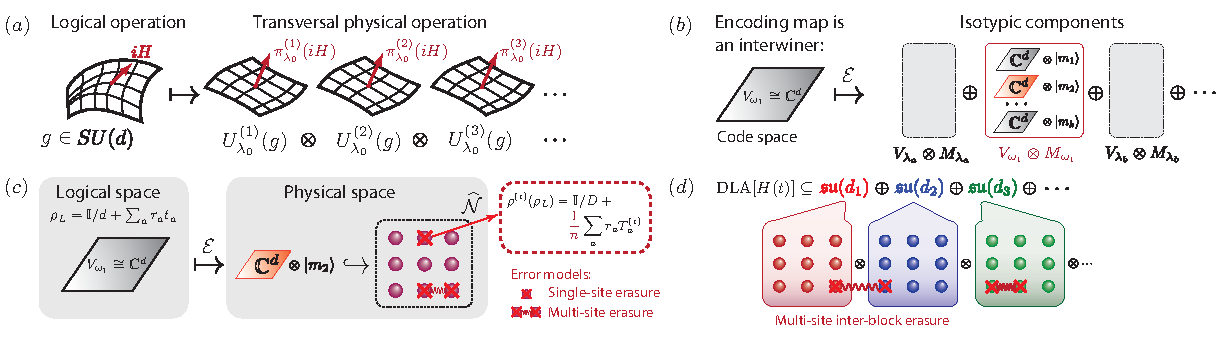
\includegraphics[width=0.7\textwidth]{figs/H_br.pdf}%
    }{%
        \fbox{\rule{0pt}{2in}\rule{0.7\textwidth}{0pt}}
    }
    \caption{Schematic illustration of objects, used in the proof of Theorem~\ref{thm:main_real}. (a) The coupling graph $\Gamma_{\mathrm{co}}$ from Definition~\ref{def:coupling_graph}. (b) Complexified Invariant algebra $\mathfrak{su}(\mathcal{H})^G$, meaning $\mathfrak{l}_{\C}$, is shown in blue blocks on diagonal (see Eq.~\eqref{eq:compl_inv_alg}); red stars represent blocks $\operatorname{Hom}(\mathcal{H}_{\alpha}, \mathcal{H}_{\beta})$, where $\mathcal{G}^{\text{br}}$ has non-zero support, corresponding to the coupling graph $\Gamma_{\mathrm{co}}$ on the left.}
    \label{fig:proof_schematic}
\end{figure}

\begin{proof}

\subsubsection*{Step 1: Complexification}

We define the complexification of the DLA in the following way:
\begin{equation}\label{eq:complexified_DLA_with_breakers}
    \mathcal{L}_{\mathbb{C}}=\mathcal{L} \otimes_{\mathbb{R}} \mathbb{C}.
\end{equation}
From now on, we will work over a complex field -- all representation theory and Lie algebraic arguments will be done in the complexified setting.

\subsubsection*{Step 2: Invariant Lie Algebra Action}

Since commutators with scalar operators are trivial, only the non-central part of the invariant algebra $\mathfrak{l}_\C$ contributes to the adjoint action on the blocks. This effective part is precisely the so-called derived algebra 
$\mathfrak{l}'_\C$, i. e.
\[
    \mathfrak{l}'_\C = [\mathfrak{l}_\C, \mathfrak{l}_\C] \cong \bigoplus_{\alpha \in \mathcal{I}} \mathrm{id}_{V_\alpha} \otimes \mathfrak{sl}\left(M_\alpha\right).
\]
Consider the action of $\mathfrak{l}'_\C$ on a specific block $\mathcal{W}_{\beta\alpha} \cong \mathbf{T}_{\beta\alpha} \otimes \mathbf{M}_{\beta\alpha}$.
Let $L \in \mathfrak{l}'_\C$. We can write $L = \sum_\gamma \id_{V_\gamma} \otimes X_\gamma$, where $X_\gamma \in \mathfrak{sl}(M_\gamma)$.
For an element $T \otimes M \in \mathcal{W}_{\beta\alpha}$ (where $T: V_\alpha \to V_\beta$ and $M: M_\alpha \rightarrow M_\beta$), the commutator is:
\begin{align*}
    [L, T \otimes M] &= (\id_{V_\beta} \otimes X_\beta)(T \otimes M) - (T \otimes M)(\id_{V_\alpha} \otimes X_\alpha) \nonumber \\
    &= T \otimes (X_\beta M - M X_\alpha).
\end{align*}
Thus, the invariant algebra acts trivially on the first factor $\mathbf{T}_{\beta\alpha}$ and acts via the representation $(X_\beta, X_\alpha) \cdot M := X_\beta M - M X_\alpha$
on the second factor $\mathbf{M}_{\beta\alpha}$, where
$(X_\beta, X_\alpha) \in \mathfrak{sl}\left(M_\beta\right) \oplus \mathfrak{sl}\left(M_\alpha\right)$.
Notice, that $\left[L, \mathcal{W}_{\beta \alpha}\right] \subseteq \mathcal{W}_{\beta \alpha}$.

\subsubsection*{Step 3: Irreducibility of Blocks.}

\begin{smlemma}
    Let $\mathfrak{g}_1, \mathfrak{g}_2$ be Lie algebras acting irreducibly on finite-dimensional vector spaces $U, V$ respectively. Then the external tensor product module $U \otimes V$ is irreducible under the action of $\mathfrak{g}_1 \oplus \mathfrak{g}_2$.
\end{smlemma}

\begin{proof}
    Let $S \subseteq U \otimes V$ be a non-zero submodule. We must show $S = U \otimes V$.
    Choose a non-zero element $x \in S$. We can write $x = \sum_{i=1}^k u_i \otimes v_i$, where $\{v_i\}$ are linearly independent in $V$. We choose $x$ such that the rank $k$ is minimal.
    
    By the Density Theorem, the action of the enveloping algebra $\mathcal{U}(\mathfrak{g}_1)$ generates all linear operators $\End(U)$. Thus, there exists an operator $L_1 \in \mathcal{U}(\mathfrak{g}_1)$ such that $L_1 u_1 = u'$ (any arbitrary vector) and $L_1 u_i = 0$ for $i > 1$.
    Applying $(L_1, 0)$ to $x$:
    \[ (L_1 \otimes \I) x = \sum (L_1 u_i) \otimes v_i = u' \otimes v_1 \in S. \]
    Since $u'$ is arbitrary, $U \otimes \{v_1\} \subseteq S$.
    
    Similarly, using the density of $\mathcal{U}(\mathfrak{g}_2)$ on $V$, we can apply $(\I \otimes L_2)$ to elements of $U \otimes \{v_1\}$ to generate $U \otimes V$. Thus $S = U \otimes V$.
\end{proof}

In our case, the derived invariant algebra $\mathfrak{l}'_\C$ contains the summand $\mathfrak{sl}(M_{\beta}) \oplus \mathfrak{sl}(M_{\alpha})$. 
The space $\mathbf{M}_{\beta\alpha} = \Hom(M_{\alpha}, M_{\beta}) \cong M_{\beta} \otimes (M_{\alpha})^*$.
Since the fundamental representation $M_{\alpha}$ and its dual $(M_{\alpha})^*$ are irreducible representations of $\mathfrak{sl}(M_{\alpha})$, the lemma implies $\mathbf{M}_{\beta\alpha}$ is irreducible.
Thus, we have the following

\begin{smlemma}\label{lem:irreducibility}
Let $\alpha,\beta\in\mathcal I$ with $\alpha\neq \beta$. Then
$
\mathbf M_{\beta\alpha}=\Hom_\C(M_\alpha,M_\beta)
$
is an irreducible module under the action of
$
\mathfrak{sl}\left(M_\beta\right) \oplus \mathfrak{sl}\left(M_\alpha\right)
$
defined by
$
(X_\beta,X_\alpha)\cdot M := X_\beta M - M X_\alpha .
$
\end{smlemma}

\subsubsection*{Step 4: Generation of off-diagonal blocks.}

\begin{smlemma}\label{prop:block_generation}
Let $\alpha,\beta\in\mathcal I$ with $\alpha\neq\beta$. Consider the
breaker-generated subspace $\mathcal B_{\beta\alpha}$ and first-factor support $S_{\beta\alpha}$, defined in Def.~\ref{def:first_factor}. Then the Lie algebra generated by
$
\mathfrak l_\C' \cup \mathcal B_{\beta\alpha}
$
contains
$
S_{\beta\alpha}\otimes \mathbf M_{\beta\alpha}.
$
In particular, if the full first-factor span condition holds on the edge $\{\alpha,\beta\}$, i.e.
$
S_{\beta\alpha}=\mathbf T_{\beta\alpha},
$
then
\[
\mathcal W_{\beta\alpha}
=
\mathbf T_{\beta\alpha}\otimes \mathbf M_{\beta\alpha}
\subseteq
\Lie_{\R}\{\mathfrak l_\C' \cup \mathcal B_{\beta\alpha}\}
\subseteq \mathcal L_\C.
\]
\end{smlemma}

\begin{proof}
Since $\alpha\neq\beta$, Lemma~\ref{lem:irreducibility} implies that $\mathbf M_{\beta\alpha}$ is an irreducible
$\mathfrak{sl}(M_\beta)\oplus \mathfrak{sl}(M_\alpha)$-module.
Therefore, for every nonzero vector $m\in \mathbf M_{\beta\alpha}$, the $\mathfrak l_\C'$-submodule generated by $m$ is all of $\mathbf M_{\beta\alpha}$. Because the action of $\mathfrak l_\C'$ is trivial on the first factor, it follows that for every simple tensor
$
t\otimes m \in \mathbf T_{\beta\alpha}\otimes \mathbf M_{\beta\alpha}
$
the $\mathfrak l_\C'$-submodule generated by $t\otimes m$ is
$
t\otimes \mathbf M_{\beta\alpha}.
$
By linearity for $\mathcal B_{\beta\alpha}$ we get that the Lie algebra generated by
$
\mathfrak l_\C' \cup \mathcal B_{\beta\alpha}
$
contains
$
S_{\beta\alpha}\otimes \mathbf M_{\beta\alpha}.
$
If the full first-factor span condition holds, then
$
S_{\beta\alpha}=\mathbf T_{\beta\alpha},
$
and therefore
\[
\mathcal W_{\beta\alpha}
=
\mathbf T_{\beta\alpha}\otimes \mathbf M_{\beta\alpha}
\subseteq
\Lie_{\R}\{\mathfrak l_\C' \cup \mathcal B_{\beta\alpha}\}.
\]
This proves the claim.
\end{proof}

\subsubsection*{Step 5: Propagation along the coupling graph $\Gamma_{\mathrm{co}}$.}

\begin{smlemma}
    $[\mathcal{W}_{\beta\gamma}, \mathcal{W}_{\gamma\alpha}] = \mathcal{W}_{\beta\alpha}$ for pairwise distinct indices.
\end{smlemma}
\begin{proof}
Let
\[
A\in \mathcal W_{\beta\gamma}=\Hom_\C(\HH_\gamma,\HH_\beta),
\qquad
B\in \mathcal W_{\gamma\alpha}=\Hom_\C(\HH_\alpha,\HH_\gamma).
\]
Then
$
AB\in \Hom_\C(\HH_\alpha,\HH_\beta)=\mathcal W_{\beta\alpha}.
$
Since \(\alpha,\beta,\gamma\) are pairwise distinct, the reverse product vanishes:
$
BA=0,
$
because \(A\) is zero outside \(\HH_\gamma\) and takes values in \(\HH_\beta\), while \(B\) is zero outside \(\HH_\alpha\), and \(\HH_\alpha\cap \HH_\beta=\{0\}\).
Hence
$
[A,B]=AB\in \mathcal W_{\beta\alpha},
$
so
$
[\mathcal W_{\beta\gamma},\mathcal W_{\gamma\alpha}]
\subseteq
\mathcal W_{\beta\alpha}.
$

For the reverse inclusion, it suffices to show that every rank-one map in
\(\mathcal W_{\beta\alpha}\) is such a commutator. Let
$
R\in \mathcal W_{\beta\alpha}=\Hom_\C(\HH_\alpha,\HH_\beta)
$
be rank one. Then there exist \(v\in \HH_\beta\) and \(u\in \HH_\alpha^*\) such that
$
R=v\otimes u.
$
Choose a nonzero vector \(w\in \HH_\gamma\), and let \(\eta\in \HH_\gamma^*\) satisfy
\(\eta(w)=1\). Define
\[
A:=v\otimes \eta \in \Hom_\C(\HH_\gamma,\HH_\beta)=\mathcal W_{\beta\gamma},
\qquad
B:=w\otimes u \in \Hom_\C(\HH_\alpha,\HH_\gamma)=\mathcal W_{\gamma\alpha}.
\]
Then
$
AB=(v\otimes \eta)(w\otimes u)=\eta(w)\,v\otimes u=R.
$
As above, \(BA=0\), and therefore
$
[A,B]=AB=R.
$
Since rank-one maps span \(\mathcal W_{\beta\alpha}\), we conclude that
$
\mathcal W_{\beta\alpha}\subseteq
[\mathcal W_{\beta\gamma},\mathcal W_{\gamma\alpha}].
$
Thus
$
[\mathcal W_{\beta\gamma},\mathcal W_{\gamma\alpha}]=\mathcal W_{\beta\alpha}.
$
\end{proof}

Since the graph $\Gamma_{\mathrm{co}}$ is connected, and we can generate the blocks corresponding to edges (by Step 4),
we can generate the block $\mathcal{W}_{\beta\alpha}$ for any pair $(\alpha, \beta)$ by taking nested commutators along a path connecting them. Thus, all off-diagonal blocks are in $\mathcal{L}_\C$.

\subsubsection*{Step 6: Generation of diagonal traceless blocks.}


\begin{smlemma}\label{lem:diag_blocks}
For any distinct \(\alpha,\beta\in\mathcal I\),
\[
[\mathcal W_{\alpha\beta},\mathcal W_{\beta\alpha}]
\subseteq
\mathcal W_{\alpha\alpha}\oplus \mathcal W_{\beta\beta}.
\]
Moreover, if \(\mathcal W_{\alpha\beta},\mathcal W_{\beta\alpha}\subseteq \mathcal L_\C\), then
their commutators generate the traceless part of
\(\mathcal W_{\alpha\alpha}\oplus \mathcal W_{\beta\beta}\).
\end{smlemma}

\begin{proof}
The inclusion is immediate from block multiplication:
\[
\mathcal W_{\alpha\beta}\mathcal W_{\beta\alpha}\subseteq \mathcal W_{\alpha\alpha},
\qquad
\mathcal W_{\beta\alpha}\mathcal W_{\alpha\beta}\subseteq \mathcal W_{\beta\beta}.
\]
Choose bases of \(\HH_\alpha\) and \(\HH_\beta\), and let
$
E^{\alpha\beta}_{ip}\in \mathcal W_{\alpha\beta},
\qquad
E^{\beta\alpha}_{qj}\in \mathcal W_{\beta\alpha}
$
be the corresponding matrix units. Then
$
[E^{\alpha\beta}_{ip},E^{\beta\alpha}_{pj}]
=
E^{\alpha\alpha}_{ij}
\qquad (i\neq j),
$
and
$
[E^{\alpha\beta}_{ip},E^{\beta\alpha}_{pi}]
=
E^{\alpha\alpha}_{ii}-E^{\beta\beta}_{pp}.
$
Thus the commutators generate all off-diagonal matrix units inside
\(\mathcal W_{\alpha\alpha}\) and \(\mathcal W_{\beta\beta}\), together with all diagonal differences. Hence they generate the traceless part of
\(\mathcal W_{\alpha\alpha}\oplus \mathcal W_{\beta\beta}\).
\end{proof}

\subsubsection*{Step 7: Descend to the Real field}

Combining the previous steps, \(\mathcal L_\C\) contains all off-diagonal blocks and the full diagonal traceless part. Hence
$
\mathcal L_\C=\mathfrak{sl}(\HH).
$ 
Since $\mathcal L_\C = \mathbb{C}\otimes_\R \mathcal L$, we have
$
\dim_\R \mathcal L=\dim_\C \mathfrak{sl}(\HH)=d^2-1.
$
But \(\mathcal L\subseteq \su(\HH)\), because it is generated by traceless skew-Hermitian operators, and
$
\dim_\R \su(\HH)=d^2-1.
$
Hence
$
\mathcal L=\su(\HH).
$
This concludes the proof of the theorem.
\end{proof}

\subsection{Applications}\label{sec:H_br_applications}
\label{sec:applications}

\subsubsection*{Example 1: $S_3$ symmetry.}

Consider the symmetric group $S_3$ acting on three qubit system $(\mathbb{C}^2)^{\otimes 3}$ by permuting them, i. e.
\[
U(\sigma)|\psi_1\rangle|\psi_2\rangle|\psi_3\rangle=|\psi_{\sigma^{-1}(1)}\rangle|\psi_{\sigma^{-1}(2)}\rangle|\psi_{\sigma^{-1}(3)}\rangle, \quad \sigma \in S_3.
\]
The Hilbert space decomposes into irreps of $S_3$ as:
\[
    \HH \cong V_{(3)} \otimes M_{(3)} \oplus V_{(2,1)} \otimes M_{(2,1)}
\]
Corresponding dimensions are
\[
    \begin{aligned}
    & \operatorname{dim} V_{(3)}=1, \quad \operatorname{dim} V_{(2,1)}=2, \\
    & \operatorname{dim} M_{(3)}=4, \quad \operatorname{dim} M_{(2,1)}=2,
    \end{aligned}
\]
The coupling graph $\Gamma_{\mathrm{co}}$ has two vertices corresponding to $(2,1)$ and $(3)$ irreps.
The relevant first-factor space is
\[
    \mathbf{T}_{(2,1),(3)}=\operatorname{Hom}\left(V_{(3)}, V_{(2,1)}\right) \cong V_{(2,1)}
\]
so $\operatorname{dim} \mathbf{T}_{(2,1),(3)}=2$. Which means that we only have to check the theorem conditions 
for one edge $(2,1)\to(3)$. Thus, a single breaker $iH_{\mathrm{br}}$ can work if projection
\[
    \Pi_{(2,1),(3)}\left(iH_{\mathrm{br}}\right) \in \mathbf{T}_{(2,1),(3)} \otimes \mathbf{M}_{(2,1),(3)}
\]
has first-factor support equal to all of $\mathbf{T}_{(2,1),(3)}$.
Let's prove that $iH^{\mathrm{br}}=iZ_1+iX_2$ is enough to achieve universality. From now on, we will work with Hamiltonians instead of skew-Hermitian generators, so we will omit the factor of $i$ for brevity. 

We first compute the block-projection explicitly
\[
    \Pi_{(2,1),(3)}(Z_1+X_2)=P_{(2,1)} (Z_1+X_2) P_{(3)}.
\]
In this example, it is much easier, because we have to compute only $P_{(3)}$, for example, and then
$P_{(2,1)}=\mathrm{1}-P_{(3)}$. We can compute $P_{(3)}$ by using Eq.~\eqref{eq:projector_formula}
\[
    P_{(3)}=\frac{1}{6}(I+U(12)+U(13)+U(23)+U(123)+U(132))
\]
Basis in $\HH_{(3)}$ isotypic component is given by the following vectors:
\[
    \begin{aligned}
    & s_0=|000\rangle, \quad s_1=\frac{|100\rangle+|010\rangle+|001\rangle}{\sqrt{3}}, \\
    & s_2=\frac{|110\rangle+|101\rangle+|011\rangle}{\sqrt{3}}, \quad s_3=|111\rangle .
    \end{aligned}
\]
As for $\HH_{(2,1)}$, we choose the following basis:
\[
    \begin{aligned}
    &u_1=\frac{2|100\rangle-|010\rangle-|001\rangle}{\sqrt{6}}, \quad u_2=\frac{|010\rangle-|001\rangle}{\sqrt{2}},\\
    &v_1=\frac{2|011\rangle-|101\rangle-|110\rangle}{\sqrt{6}}, \quad v_2=\frac{|101\rangle-|110\rangle}{\sqrt{2}},
    \end{aligned}
\]
Knowing the action of $Z_1$, $X_2$ and $P_{(3)}$ on the computational basis, we can compute the matrix representation of $\Pi_{(2,1),(3)}(Z_1+X_2)$ in the bases defined above. We get
\[
    \left[\Pi_{(2,1),(3)}(Z_1+X_2)\right]_{\left(u_1, v_1, u_2, v_2\right) \leftarrow\left(s_0, s_1, s_2, s_3\right)}=\left(\begin{array}{cccc}
    -\frac{\sqrt{6}}{6} & -\frac{2 \sqrt{2}}{3} & \frac{\sqrt{2}}{6} & 0 \\
    0 & \frac{\sqrt{2}}{6} & \frac{2 \sqrt{2}}{3} & -\frac{\sqrt{6}}{6} \\
    \frac{\sqrt{2}}{2} & 0 & -\frac{\sqrt{6}}{6} & 0 \\
    0 & -\frac{\sqrt{6}}{6} & 0 & \frac{\sqrt{2}}{2}
    \end{array}\right).
\]
We choose a basis $\left\{e_1, e_2\right\}$ of $V_{(2,1)}$ and a basis $\left\{m_1, m_2\right\}$ of the multiplicity space $M_{(2,1)}$, and identify 
\[
    u_1=e_1 \otimes m_1, \quad u_2=e_2 \otimes m_1, \quad v_1=e_1 \otimes m_2, \quad v_2=e_2 \otimes m_2,
\]
from which it becomes apparent that
\[
    \Pi_{(2,1),(3)}(Z_1+X_2)=e_1 \otimes F_1+e_2 \otimes F_2,
\]
where $F_1, F_2 \in \mathbf{M}_{(2,1),(3)}=\operatorname{Hom}\left(M_{(3)}, M_{(2,1)}\right)$ such that
\[
    \begin{gathered}
    F_1=\left(\begin{array}{cccc}
    -\frac{\sqrt{6}}{6} & -\frac{2 \sqrt{2}}{3} & \frac{\sqrt{2}}{6} & 0 \\
    0 & \frac{\sqrt{2}}{6} & \frac{2 \sqrt{2}}{3} & -\frac{\sqrt{6}}{6}
    \end{array}\right), \\
    F_2=\left(\begin{array}{cccc}
    \frac{\sqrt{2}}{2} & 0 & -\frac{\sqrt{6}}{6} & 0 \\
    0 & -\frac{\sqrt{6}}{6} & 0 & \frac{\sqrt{2}}{2}
    \end{array}\right) .
    \end{gathered}
\]  
Notice that $e_1$ and $e_2$ are linearly independent by construction. $F_1$ and $F_2$ are linearly independent, so breaker satisfies the full first-factor span condition, i. e.
\[
    S_{(2,1),(3)}=\operatorname{span}\left\{e_1, e_2\right\}=\mathbf{T}_{(2,1),(3)}.
\]
We conclude that
\[
    \Lie_{\R}\left\{\mathfrak{su}\left((\mathbb{C}^2)^{\otimes 3}\right)^{S_3} \cup\{iZ_1+iX_2\}\right\}=\mathfrak{su}\left((\mathbb{C}^2)^{\otimes 3}\right).
\]

\begin{smremark}
    The proof would be simpler if we split the $Z_1+X_2$ Hamiltonian into two breakers, i. e. consider the breaking set $\mathcal{G}^{\text {br }}=\left\{i Z_1, i X_2\right\}$. Indeed, with two breakers, one only needs independence of the first-factor directions; however, with one combined breaker, one also needs independence on the multiplicity side to check the full first-factor span condition.
    Without linear independence of $F_1$ and $F_2$, the breaker would be $\Pi_{(2,1),(3)}(Z_1+X_2)=(e_1+ \lambda e_2) \otimes F_1$,
    so the first-factor support would be only one-dimensional, despite $e_1$ and $e_2$ being linearly independent.
\end{smremark}


\end{appendix}

\end{document}